% !TeX program = xelatex
% !TeX encoding = UTF-8
% Presentazione revisionata: Locus: statistica spaziale
% Basata sul materiale originale fornito dall'autore e sul template M01_Pensare_con_i_dati.tex
% Compilazione: xelatex -interaction=nonstopmode Locus_M11_statistica_spaziale.tex (due passaggi)
% Diagrammi TikZ e figure statistiche vettoriali; sorgenti R e dati inclusi.
% Revisione completa delle 110 slide; fonti consultate il 20 novembre 2026.
\documentclass[12pt,aspectratio=1610]{beamer}
\geometry{paperwidth=20cm,paperheight=12.5cm}
\usepackage[italian,provide=*]{babel}
\usepackage{fontspec}
\IfFontExistsTF{NimbusSans-Regular.otf}{
\setsansfont{NimbusSans-Regular.otf}[BoldFont=NimbusSans-Bold.otf,ItalicFont=NimbusSans-Italic.otf,BoldItalicFont=NimbusSans-BoldItalic.otf]
\setmainfont{NimbusSans-Regular.otf}[BoldFont=NimbusSans-Bold.otf,ItalicFont=NimbusSans-Italic.otf,BoldItalicFont=NimbusSans-BoldItalic.otf]
}{
\setsansfont{TeX Gyre Heros}
\setmainfont{TeX Gyre Heros}
}
\IfFontExistsTF{DejaVu Sans Mono}{
\setmonofont{DejaVu Sans Mono}[Scale=.88]
}{\setmonofont{Latin Modern Mono}[Scale=.88]}
\usefonttheme{professionalfonts}
\usepackage{amsmath,amssymb,booktabs,array,graphicx,tikz,bookmark}
\usetikzlibrary{calc,positioning,arrows.meta}
\graphicspath{{Risorse/Figure/}}
\definecolor{Paper}{HTML}{F8F6F1}
\definecolor{Ink}{HTML}{253344}
\definecolor{Navy}{HTML}{15283E}
\definecolor{Quantum}{HTML}{5146A5}
\definecolor{Classical}{HTML}{087C74}
\definecolor{Muted}{HTML}{657180}
\definecolor{Rule}{HTML}{D6DAD9}
\definecolor{Night}{HTML}{112236}
\definecolor{Lilac}{HTML}{ABB5FF}
\definecolor{Mint}{HTML}{72D8C8}
\setbeamercolor{background canvas}{bg=Paper}
\setbeamercolor{normal text}{fg=Ink}
\setbeamertemplate{navigation symbols}{}
\setbeamertemplate{headline}{}
\setbeamertemplate{footline}{}
\setbeamersize{text margin left=0pt,text margin right=0pt}
\hypersetup{colorlinks=true,linkcolor=Classical,urlcolor=Classical,pdfpagemode=UseOutlines,pdfstartview=Fit,
 pdftitle={Locus: statistica spaziale},pdfauthor={Marzio De Corato},
 pdfsubject={Modulo M11: coordinate, associazione e previsione nel territorio, Revisione completa: diagrammi TikZ, formule e codice R commentato}}
\bookmarksetup{open,openlevel=0,depth=2}
\newsavebox{\BodyBox}
\newsavebox{\SideBox}
\newsavebox{\RecallBox}
\newsavebox{\TitleBox}
\newcommand{\MeasureBox}[2]{\typeout{REVIEWBOX:#1:\the\wd#2:\the\ht#2:\the\dp#2}}

% Revisione completa: diagrammi TikZ, formalismo e box R.
\usepackage[most]{tcolorbox}
\usepackage{listings}
\usetikzlibrary{fit,backgrounds,matrix,decorations.pathreplacing}
\definecolor{GeoA}{HTML}{1D7890}
\definecolor{GeoB}{HTML}{C57E42}
\definecolor{GeoC}{HTML}{7363AA}
\definecolor{GeoTint}{HTML}{F0F4F3}
\lstdefinestyle{GeoR}{language=R,basicstyle=\ttfamily\fontsize{9.2}{12.2}\selectfont,
 keywordstyle=\color{Quantum}\bfseries,commentstyle=\color{Classical},stringstyle=\color{GeoB},
 numbers=left,numberstyle=\tiny\color{Muted},numbersep=4pt,showstringspaces=false,
 columns=fullflexible,keepspaces=true,breaklines=true,xleftmargin=1.15em,
 frame=none,aboveskip=0pt,belowskip=0pt,tabsize=2}
\newsavebox{\PilotLeftBox}
\newsavebox{\PilotRightBox}
\newcommand{\PLabel}[1]{\par{\color{Classical}\bfseries\fontsize{9}{11}\selectfont\MakeUppercase{#1}}\par\vspace{1.8mm}}
\newcommand{\PBody}[1]{\par{\fontsize{11.3}{14.8}\selectfont #1\par}}
\newcommand{\PSmall}[1]{\par{\fontsize{9.8}{13.1}\selectfont #1\par}}
\newcommand{\PCode}[2]{%
\begin{tcolorbox}[enhanced,arc=1.8mm,boxrule=.65pt,
  colback=white,colframe=Classical!75!Navy,colbacktitle=Navy,
  coltitle=white,fonttitle=\bfseries\fontsize{9.6}{12}\selectfont,
  title={#1},left=1.7mm,right=1.3mm,top=1.5mm,bottom=1.3mm,
  before skip=1mm,after skip=1mm]
\lstinputlisting[style=GeoR]{Codice/#2}
\end{tcolorbox}}
\newcommand{\PInfo}[1]{%
\begin{tcolorbox}[enhanced,arc=1.6mm,boxrule=.55pt,colback=GeoTint,
 colframe=Rule!80!Classical,left=2.3mm,right=2.3mm,top=2mm,bottom=2mm,
 before skip=1mm,after skip=1mm]
\PSmall{#1}\end{tcolorbox}}
\tikzset{
 pFlow/.style={draw=Classical!45,fill=white,rounded corners=2mm,
  line width=.7pt,align=center,minimum height=1.1cm,font=\sffamily\fontsize{10}{12}\selectfont},
 pEdge/.style={-{Latex[length=2.3mm]},draw=Classical,line width=.95pt},
 pGroup/.style={draw=Rule,fill=white,rounded corners=2mm,line width=.65pt},
 pDotA/.style={circle,fill=GeoA,inner sep=1.25pt},
 pDotB/.style={circle,fill=GeoB,inner sep=1.25pt},
 pDotC/.style={circle,fill=GeoC,inner sep=1.25pt}
}
\newcommand{\PilotChrome}[4]{%
  \node[anchor=north west,inner sep=0,text width=17.7cm] at ([xshift=.95cm,yshift=-.55cm]current page.north west) {\color{Navy}\bfseries\fontsize{20.6}{24.5}\selectfont #1};
  \node[anchor=north east,inner sep=0] at ([xshift=19.05cm,yshift=-.14cm]current page.north west) {\color{Classical}\fontsize{8}{10}\selectfont\hyperlink{slide2}{#2}};
  \draw[Classical,line width=1.2pt] ([xshift=.95cm,yshift=-1.7cm]current page.north west)--([xshift=2.35cm,yshift=-1.7cm]current page.north west);
  \draw[Rule,line width=.65pt] ([xshift=.95cm,yshift=-10.36cm]current page.north west)--([xshift=19.05cm,yshift=-10.36cm]current page.north west);
  \node[anchor=north west,inner sep=0] at ([xshift=.96cm,yshift=-10.55cm]current page.north west) {\color{Classical}\bfseries\fontsize{9.1}{12}\selectfont DA RICORDARE};
  \node[anchor=north west,inner sep=0,text width=14.3cm] at ([xshift=4.2cm,yshift=-10.53cm]current page.north west) {\color{Ink}\fontsize{10.3}{13.8}\selectfont #4};
  \draw[Rule,line width=.35pt] ([xshift=.95cm,yshift=-11.92cm]current page.north west)--([xshift=19.05cm,yshift=-11.92cm]current page.north west);
  \node[anchor=north west,inner sep=0] at ([xshift=.95cm,yshift=-12.06cm]current page.north west) {\color{Muted}\fontsize{7.7}{9.2}\selectfont Locus: statistica spaziale};
  \node[anchor=north east,inner sep=0] at ([xshift=19.05cm,yshift=-12.06cm]current page.north west) {\color{Muted}\fontsize{7.7}{9.2}\selectfont #3/110};
}


% Stili comuni per i diagrammi scientifici della revisione completa.
\tikzset{
 pAxis/.style={-{Latex[length=2mm]},draw=Muted,line width=.65pt},
 pNote/.style={font=\sffamily\fontsize{9}{11.5}\selectfont,text=Muted,align=center},
 pLabel/.style={font=\sffamily\fontsize{10}{12.5}\selectfont,text=Ink,align=center}
}
\newsavebox{\FullWideBox}
\setlength{\emergencystretch}{1em}




\newcommand{\PLab}[2]{\par{\color{Classical}\bfseries\fontsize{9}{11}\selectfont
\href{#1}{\MakeUppercase{#2}}}\par\vspace{1.8mm}}


\begin{document}

\begin{frame}[plain]\hypertarget{slide1}{}\bookmark[level=0,page=1]{Locus}
\begin{tikzpicture}[remember picture,overlay]
\fill[Night](current page.south west) rectangle(current page.north east);
\IfFileExists{Risorse/Copertine/M11_Locus.jpg}{\node[inner sep=0] at(current page.center){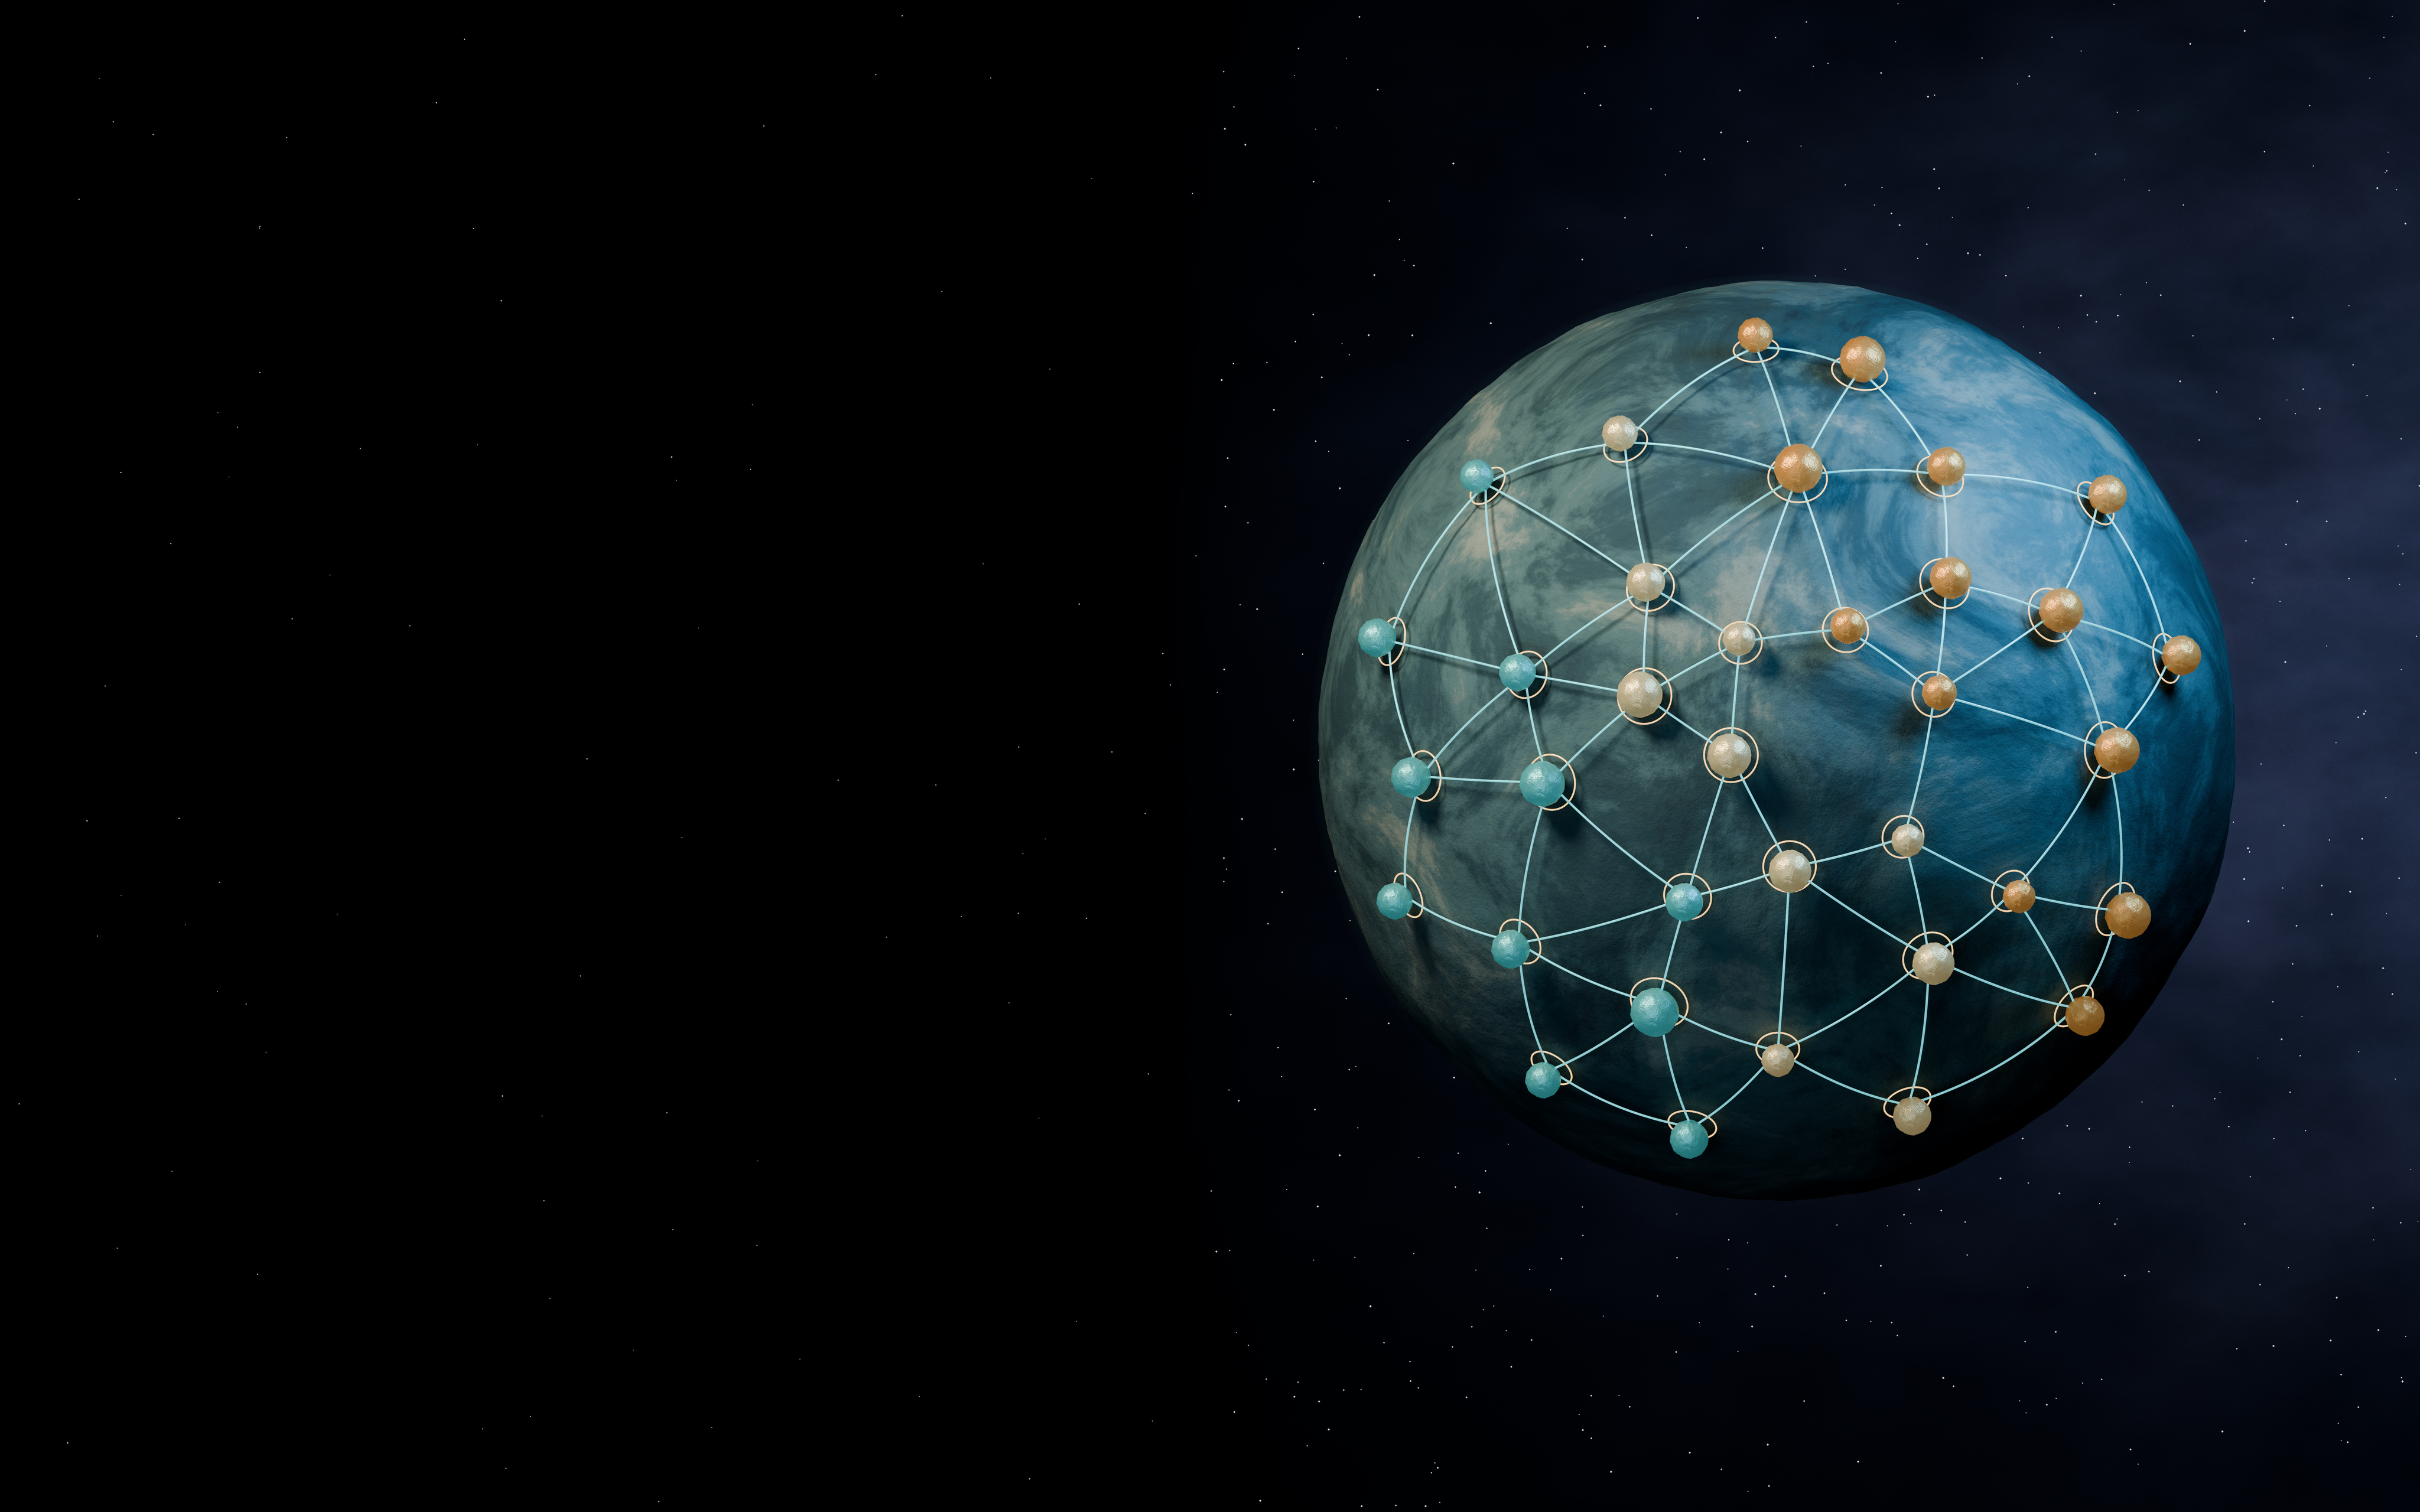
\includegraphics[width=20cm,height=12.5cm]{Risorse/Copertine/M11_Locus.jpg}};}{}
\node[anchor=north west,inner sep=0] at([xshift=1.05cm,yshift=-1.10cm]current page.north west){\color{Mint}\bfseries\fontsize{23}{28}\selectfont LOCUS};
\node[anchor=north west,inner sep=0] at([xshift=1.07cm,yshift=-2.16cm]current page.north west){\color{white}\fontsize{9}{12}\selectfont MODULO M11 · SCIENZE DELLA TERRA};
\draw[Mint,line width=1.5pt]([xshift=1.07cm,yshift=-2.78cm]current page.north west)--([xshift=2.6cm,yshift=-2.78cm]current page.north west);
\node[anchor=north west,inner sep=0] at([xshift=1.05cm,yshift=-3.35cm]current page.north west){\begin{minipage}{9.2cm}\raggedright\color{white}\bfseries\fontsize{30}{36}\selectfont Statistica\\spaziale\end{minipage}};
\node[anchor=north west,inner sep=0] at([xshift=1.07cm,yshift=-7.88cm]current page.north west){\begin{minipage}{8.9cm}\raggedright\color{Lilac}\fontsize{12.2}{17}\selectfont Coordinate, associazione\\e previsione nel territorio\end{minipage}};
\node[anchor=north west,inner sep=0] at([xshift=1.07cm,yshift=-10.52cm]current page.north west){\color{white}\fontsize{11.5}{15}\selectfont Marzio De Corato};
\node[anchor=north west,inner sep=0] at([xshift=1.07cm,yshift=-11.17cm]current page.north west){\color{Mint}\fontsize{8.8}{11}\selectfont\href{https://creativecommons.org/licenses/by-nc-sa/4.0/}{© 2026 · CC BY-NC-SA 4.0}};
\end{tikzpicture}\end{frame}
\begin{frame}[plain]\hypertarget{slide2}{}
\bookmark[level=0,page=2]{I · DATO E SUPPORTO}
\bookmark[level=1,page=2]{Dai campioni alle relazioni spaziali}
\begin{lrbox}{\TitleBox}
\begin{minipage}[t]{17.7cm}\raggedright\color{Ink}\fontsize{11.3}{14.8}\selectfont
\color{Navy}\bfseries\fontsize{20.6}{24.5}\selectfont Dai campioni alle relazioni spaziali
\end{minipage}\end{lrbox}
\typeout{FULLBOX:002:TitleBox:\the\ht\TitleBox:\the\dp\TitleBox}

\begin{lrbox}{\RecallBox}
\begin{minipage}[t]{14.3cm}\raggedright\color{Ink}\fontsize{11.3}{14.8}\selectfont
\fontsize{10.3}{13.8}\selectfont Prima di calcolare una relazione spaziale, bisogna dichiarare che cosa rappresentano i campioni.
\end{minipage}\end{lrbox}
\typeout{FULLBOX:002:RecallBox:\the\ht\RecallBox:\the\dp\RecallBox}

\begin{lrbox}{\PilotLeftBox}
\begin{minipage}[t]{10.05cm}\raggedright\color{Ink}\fontsize{11.3}{14.8}\selectfont
\PLabel{Il percorso di Locus}
{\fontsize{10.2}{13.1}\selectfont\renewcommand{\arraystretch}{1.45}\begin{tabular}{@{}p{8.3cm}p{0.7cm}@{}}\toprule
\textbf{Passaggio} & \textbf{p.}\\\midrule
\hyperlink{slide5}{Definire dato e supporto} & 5\\
\hyperlink{slide17}{Leggere coordinate e distanze} & 17\\
\hyperlink{slide32}{Costruire carte e appartenenze} & 32\\
\hyperlink{slide44}{Dichiarare vicinati e pesi} & 44\\
\hyperlink{slide56}{Misurare l’associazione spaziale} & 56\\
\hyperlink{slide71}{Studiare la semivarianza} & 71\\
\hyperlink{slide82}{Valutare la copertura del campione} & 82\\
\hyperlink{slide92}{Prevedere e verificare nello spazio} & 92\\
\hyperlink{slide106}{Consegnare un’analisi riproducibile} & 106\\
\bottomrule\end{tabular}}

\end{minipage}\end{lrbox}
\typeout{FULLBOX:002:PilotLeftBox:\the\ht\PilotLeftBox:\the\dp\PilotLeftBox}

\begin{lrbox}{\PilotRightBox}
\begin{minipage}[t]{7.55cm}\raggedright\color{Ink}\fontsize{11.3}{14.8}\selectfont
\PBody{Futura ha collegato previsione e verifica temporale. Locus applica lo stesso rigore a posizioni, relazioni di vicinato e aree lasciate fuori dalla stima.}
\vspace{2.5mm}
\PInfo{Il caso guida comprende 64 siti sintetici. Le misure di concentrazione sono espresse in unità arbitrarie; le coordinate locali sono in metri.}
\PBody{I 20 notebook mantengono gli identificativi M11\_N01--M11\_N20 del sito. Ogni attività contiene codice, risultati eseguiti e interpretazione.}
\vspace{2.5mm}

\end{minipage}\end{lrbox}
\typeout{FULLBOX:002:PilotRightBox:\the\ht\PilotRightBox:\the\dp\PilotRightBox}

\begin{tikzpicture}[remember picture,overlay]
\PilotChrome{Dai campioni alle relazioni spaziali}{I · DATO E SUPPORTO}{2}{Prima di calcolare una relazione spaziale, bisogna dichiarare che cosa rappresentano i campioni.}
\node[anchor=north west,inner sep=0] at([xshift=.96cm,yshift=-2.13cm]current page.north west){\usebox{\PilotLeftBox}};
\node[anchor=north west,inner sep=0] at([xshift=11.52cm,yshift=-2.13cm]current page.north west){\usebox{\PilotRightBox}};
\end{tikzpicture}\end{frame}

\begin{frame}[plain]\hypertarget{slide3}{}
\bookmark[level=1,page=3]{Dal tempo alle posizioni sul territorio}
\begin{lrbox}{\TitleBox}
\begin{minipage}[t]{17.7cm}\raggedright\color{Ink}\fontsize{11.3}{14.8}\selectfont
\color{Navy}\bfseries\fontsize{20.6}{24.5}\selectfont Dal tempo alle posizioni sul territorio
\end{minipage}\end{lrbox}
\typeout{FULLBOX:003:TitleBox:\the\ht\TitleBox:\the\dp\TitleBox}

\begin{lrbox}{\RecallBox}
\begin{minipage}[t]{14.3cm}\raggedright\color{Ink}\fontsize{11.3}{14.8}\selectfont
\fontsize{10.3}{13.8}\selectfont Nello spazio occorre costruire la nozione di vicino prima di usare un modello di dipendenza.
\end{minipage}\end{lrbox}
\typeout{FULLBOX:003:RecallBox:\the\ht\RecallBox:\the\dp\RecallBox}

\begin{lrbox}{\PilotLeftBox}
\begin{minipage}[t]{10.05cm}\raggedright\color{Ink}\fontsize{11.3}{14.8}\selectfont
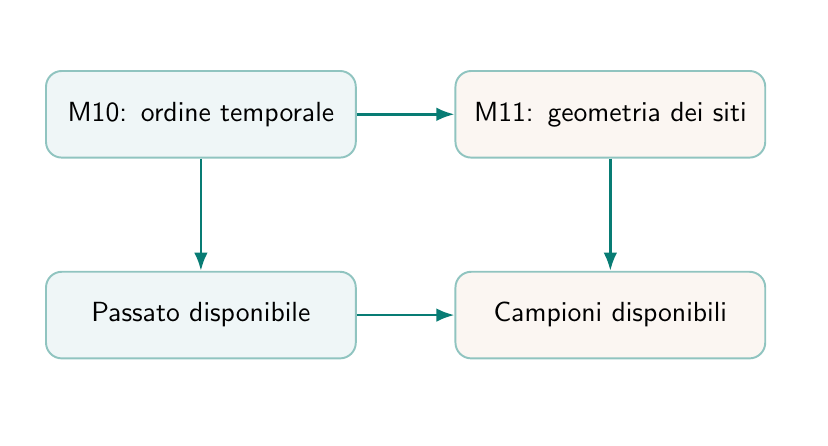
\begin{tikzpicture}[x=1cm,y=1cm]
\path[use as bounding box](-.1,-.15) rectangle(9.7,4.8);
\node[pFlow,text width=3.7cm,fill=GeoA!7] (a) at(2.1,3.7){M10: ordine temporale};
\node[pFlow,text width=3.7cm,fill=GeoB!7] (b) at(7.3,3.7){M11: geometria dei siti};
\node[pFlow,text width=3.7cm,fill=GeoA!7] (c) at(2.1,1.15){Passato disponibile};
\node[pFlow,text width=3.7cm,fill=GeoB!7] (d) at(7.3,1.15){Campioni disponibili};
\draw[pEdge] (a) -- (b);
\draw[pEdge] (a) -- (c);
\draw[pEdge] (b) -- (d);
\draw[pEdge] (c) -- (d);
\end{tikzpicture}
\[Y_t\quad\longrightarrow\quad Z(s),\qquad s\in D\subset\mathbb R^2\]

\end{minipage}\end{lrbox}
\typeout{FULLBOX:003:PilotLeftBox:\the\ht\PilotLeftBox:\the\dp\PilotLeftBox}

\begin{lrbox}{\PilotRightBox}
\begin{minipage}[t]{7.55cm}\raggedright\color{Ink}\fontsize{11.3}{14.8}\selectfont
\PBody{Nel tempo esiste un ordine naturale. Nello spazio la vicinanza richiede una metrica, una scala e talvolta una direzione.}
\vspace{2.5mm}
\PInfo{Due siti separati dalla stessa distanza possono appartenere a versanti, litologie o bacini diversi. La distanza geometrica non esaurisce la relazione scientifica.}
\PBody{La previsione resta legata all’informazione disponibile: la geometria dei punti tenuti fuori deve rappresentare il compito da valutare.}
\vspace{2.5mm}

\end{minipage}\end{lrbox}
\typeout{FULLBOX:003:PilotRightBox:\the\ht\PilotRightBox:\the\dp\PilotRightBox}

\begin{tikzpicture}[remember picture,overlay]
\PilotChrome{Dal tempo alle posizioni sul territorio}{I · DATO E SUPPORTO}{3}{Nello spazio occorre costruire la nozione di vicino prima di usare un modello di dipendenza.}
\node[anchor=north west,inner sep=0] at([xshift=.96cm,yshift=-2.13cm]current page.north west){\usebox{\PilotLeftBox}};
\node[anchor=north west,inner sep=0] at([xshift=11.52cm,yshift=-2.13cm]current page.north west){\usebox{\PilotRightBox}};
\end{tikzpicture}\end{frame}

\begin{frame}[plain]\hypertarget{slide4}{}
\bookmark[level=1,page=4]{Quale domanda deve risolvere la carta?}
\begin{lrbox}{\TitleBox}
\begin{minipage}[t]{17.7cm}\raggedright\color{Ink}\fontsize{11.3}{14.8}\selectfont
\color{Navy}\bfseries\fontsize{20.6}{24.5}\selectfont Quale domanda deve risolvere la carta?
\end{minipage}\end{lrbox}
\typeout{FULLBOX:004:TitleBox:\the\ht\TitleBox:\the\dp\TitleBox}

\begin{lrbox}{\RecallBox}
\begin{minipage}[t]{14.3cm}\raggedright\color{Ink}\fontsize{11.3}{14.8}\selectfont
\fontsize{10.3}{13.8}\selectfont La domanda scientifica stabilisce quali distanze, supporti e verifiche servono.
\end{minipage}\end{lrbox}
\typeout{FULLBOX:004:RecallBox:\the\ht\RecallBox:\the\dp\RecallBox}

\begin{lrbox}{\PilotLeftBox}
\begin{minipage}[t]{10.05cm}\raggedright\color{Ink}\fontsize{11.3}{14.8}\selectfont
{\fontsize{10.2}{13.1}\selectfont\renewcommand{\arraystretch}{1.45}\begin{tabular}{@{}p{4.5cm}p{4.5cm}@{}}\toprule
\textbf{Domanda} & \textbf{Oggetto da dichiarare}\\\midrule
Dove sono le misure? & Posizione, unità e copertura\\
Quali siti si assomigliano? & Vicinato e riferimento inferenziale\\
Quanto cambia il fenomeno? & Distanza, direzione e supporto\\
Che cosa prevedo altrove? & Bersaglio e verifica geografica\\
\bottomrule\end{tabular}}

\end{minipage}\end{lrbox}
\typeout{FULLBOX:004:PilotLeftBox:\the\ht\PilotLeftBox:\the\dp\PilotLeftBox}

\begin{lrbox}{\PilotRightBox}
\begin{minipage}[t]{7.55cm}\raggedright\color{Ink}\fontsize{11.3}{14.8}\selectfont
\PBody{Una carta può descrivere campioni, confrontare aree oppure mostrare previsioni. Sono operazioni che richiedono dati e assunzioni differenti.}
\vspace{2.5mm}
\PInfo{Nel caso guida prevediamo la concentrazione in siti a Est usando solo i campioni a Ovest. Il protocollo separa questa verifica dalle carte descrittive dell’intero insieme.}
\PBody{La copertina richiama campioni e connessioni. Nelle figure scientifiche ogni collegamento avrà una regola esplicita.}
\vspace{2.5mm}

\end{minipage}\end{lrbox}
\typeout{FULLBOX:004:PilotRightBox:\the\ht\PilotRightBox:\the\dp\PilotRightBox}

\begin{tikzpicture}[remember picture,overlay]
\PilotChrome{Quale domanda deve risolvere la carta?}{I · DATO E SUPPORTO}{4}{La domanda scientifica stabilisce quali distanze, supporti e verifiche servono.}
\node[anchor=north west,inner sep=0] at([xshift=.96cm,yshift=-2.13cm]current page.north west){\usebox{\PilotLeftBox}};
\node[anchor=north west,inner sep=0] at([xshift=11.52cm,yshift=-2.13cm]current page.north west){\usebox{\PilotRightBox}};
\end{tikzpicture}\end{frame}

\begin{frame}[plain]\hypertarget{slide5}{}
\bookmark[level=1,page=5]{Il caso guida: 64 siti sintetici}
\begin{lrbox}{\TitleBox}
\begin{minipage}[t]{17.7cm}\raggedright\color{Ink}\fontsize{11.3}{14.8}\selectfont
\color{Navy}\bfseries\fontsize{20.6}{24.5}\selectfont Il caso guida: 64 siti sintetici
\end{minipage}\end{lrbox}
\typeout{FULLBOX:005:TitleBox:\the\ht\TitleBox:\the\dp\TitleBox}

\begin{lrbox}{\RecallBox}
\begin{minipage}[t]{14.3cm}\raggedright\color{Ink}\fontsize{11.3}{14.8}\selectfont
\fontsize{10.3}{13.8}\selectfont I dati sintetici sono un esperimento didattico: le loro unità e la loro origine restano esplicite.
\end{minipage}\end{lrbox}
\typeout{FULLBOX:005:RecallBox:\the\ht\RecallBox:\the\dp\RecallBox}

\begin{lrbox}{\PilotLeftBox}
\begin{minipage}[t]{10.05cm}\raggedright\color{Ink}\fontsize{11.3}{14.8}\selectfont
{\fontsize{10.2}{13.1}\selectfont\renewcommand{\arraystretch}{1.45}\begin{tabular}{@{}p{3.6cm}p{5.5cm}@{}}\toprule
\textbf{Campo} & \textbf{Significato}\\\midrule
\texttt{id} & Identificativo stabile S01--S64\\
\texttt{x\_m}, \texttt{y\_m} & Piano locale, metri, passo 250 m\\
\texttt{concentrazione} & Variabile sintetica, unità arbitrarie\\
\texttt{quota\_m} & Quota sintetica in metri\\
\texttt{lon}, \texttt{lat} & Coordinate geografiche sintetiche\\
\texttt{area} & Ovest/Est con soglia a 1000 m\\
\bottomrule\end{tabular}}

\end{minipage}\end{lrbox}
\typeout{FULLBOX:005:PilotLeftBox:\the\ht\PilotLeftBox:\the\dp\PilotLeftBox}

\begin{lrbox}{\PilotRightBox}
\begin{minipage}[t]{7.55cm}\raggedright\color{Ink}\fontsize{11.3}{14.8}\selectfont
\PBody{La griglia contiene otto posizioni per asse, da 0 a 1750 m. Il dataset permette di seguire gli stessi campioni attraverso tutte le operazioni.}
\vspace{2.5mm}
\PInfo{Il piano locale ha un’origine convenzionale. Il nome della colonna e l’unità metro non autorizzano ad assegnargli un codice EPSG.}
\PSmall{Il file originale, la revisione Git e le impronte dei dati accompagnano il pacchetto. Nessun risultato richiede un download durante la lettura.}

\end{minipage}\end{lrbox}
\typeout{FULLBOX:005:PilotRightBox:\the\ht\PilotRightBox:\the\dp\PilotRightBox}

\begin{tikzpicture}[remember picture,overlay]
\PilotChrome{Il caso guida: 64 siti sintetici}{I · DATO E SUPPORTO}{5}{I dati sintetici sono un esperimento didattico: le loro unità e la loro origine restano esplicite.}
\node[anchor=north west,inner sep=0] at([xshift=.96cm,yshift=-2.13cm]current page.north west){\usebox{\PilotLeftBox}};
\node[anchor=north west,inner sep=0] at([xshift=11.52cm,yshift=-2.13cm]current page.north west){\usebox{\PilotRightBox}};
\node[anchor=north east,inner sep=0] at([xshift=17.65cm,yshift=-12.06cm]current page.north west){\color{Classical}\fontsize{7.7}{9.2}\selectfont\href{../../03_Notebook_svolti/M11_Locus/M11_N01.html}{M11\_N01 · notebook svolto}};
\end{tikzpicture}\end{frame}

\begin{frame}[plain]\hypertarget{slide6}{}
\bookmark[level=1,page=6]{Valore, posizione e supporto formano il dato}
\begin{lrbox}{\TitleBox}
\begin{minipage}[t]{17.7cm}\raggedright\color{Ink}\fontsize{11.3}{14.8}\selectfont
\color{Navy}\bfseries\fontsize{20.6}{24.5}\selectfont Valore, posizione e supporto formano il dato
\end{minipage}\end{lrbox}
\typeout{FULLBOX:006:TitleBox:\the\ht\TitleBox:\the\dp\TitleBox}

\begin{lrbox}{\RecallBox}
\begin{minipage}[t]{14.3cm}\raggedright\color{Ink}\fontsize{11.3}{14.8}\selectfont
\fontsize{10.3}{13.8}\selectfont Una coordinata da sola non descrive il processo con cui il valore è stato misurato.
\end{minipage}\end{lrbox}
\typeout{FULLBOX:006:RecallBox:\the\ht\RecallBox:\the\dp\RecallBox}

\begin{lrbox}{\PilotLeftBox}
\begin{minipage}[t]{10.05cm}\raggedright\color{Ink}\fontsize{11.3}{14.8}\selectfont
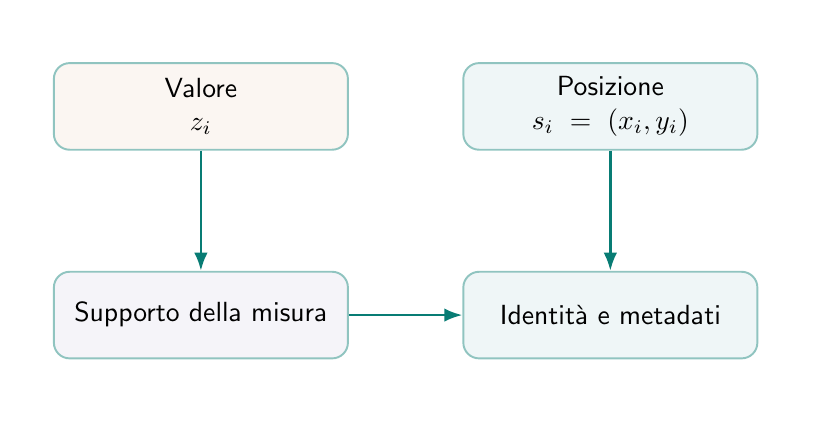
\begin{tikzpicture}[x=1cm,y=1cm]
\path[use as bounding box](-.1,-.15) rectangle(9.7,4.8);
\node[pFlow,text width=3.5cm,fill=GeoB!7] (a) at(2.1,3.8){Valore\\$z_i$};
\node[pFlow,text width=3.5cm,fill=GeoA!7] (b) at(7.3,3.8){Posizione\\$s_i=(x_i,y_i)$};
\node[pFlow,text width=3.5cm,fill=GeoC!7] (c) at(2.1,1.15){Supporto della misura};
\node[pFlow,text width=3.5cm,fill=GeoA!7] (d) at(7.3,1.15){Identità e metadati};
\draw[pEdge] (a) -- (c);
\draw[pEdge] (b) -- (d);
\draw[pEdge] (c) -- (d);
\end{tikzpicture}
\[\mathcal D=\{(\mathrm{id}_i,s_i,B_i,z_i)\}_{i=1}^{n}\]

\end{minipage}\end{lrbox}
\typeout{FULLBOX:006:PilotLeftBox:\the\ht\PilotLeftBox:\the\dp\PilotLeftBox}

\begin{lrbox}{\PilotRightBox}
\begin{minipage}[t]{7.55cm}\raggedright\color{Ink}\fontsize{11.3}{14.8}\selectfont
\PBody{La posizione è il riferimento geometrico. Il supporto è la porzione di spazio e, quando rilevante, di tempo a cui si riferisce la misura.}
\vspace{2.5mm}
\PInfo{Una carota, una porzione di suolo e la media di un bacino possono avere lo stesso numero come valore. Non rappresentano la stessa quantità.}
\PBody{Identificativo e metadati permettono di riconoscere la misura dopo ordinamenti, proiezioni e join.}
\vspace{2.5mm}

\end{minipage}\end{lrbox}
\typeout{FULLBOX:006:PilotRightBox:\the\ht\PilotRightBox:\the\dp\PilotRightBox}

\begin{tikzpicture}[remember picture,overlay]
\PilotChrome{Valore, posizione e supporto formano il dato}{I · DATO E SUPPORTO}{6}{Una coordinata da sola non descrive il processo con cui il valore è stato misurato.}
\node[anchor=north west,inner sep=0] at([xshift=.96cm,yshift=-2.13cm]current page.north west){\usebox{\PilotLeftBox}};
\node[anchor=north west,inner sep=0] at([xshift=11.52cm,yshift=-2.13cm]current page.north west){\usebox{\PilotRightBox}};
\end{tikzpicture}\end{frame}

\begin{frame}[plain]\hypertarget{slide7}{}
\bookmark[level=1,page=7]{La carta iniziale mostra ciò che osserviamo}
\begin{lrbox}{\TitleBox}
\begin{minipage}[t]{17.7cm}\raggedright\color{Ink}\fontsize{11.3}{14.8}\selectfont
\color{Navy}\bfseries\fontsize{20.6}{24.5}\selectfont La carta iniziale mostra ciò che osserviamo
\end{minipage}\end{lrbox}
\typeout{FULLBOX:007:TitleBox:\the\ht\TitleBox:\the\dp\TitleBox}

\begin{lrbox}{\RecallBox}
\begin{minipage}[t]{14.3cm}\raggedright\color{Ink}\fontsize{11.3}{14.8}\selectfont
\fontsize{10.3}{13.8}\selectfont Una carta di punti deve rendere visibili i campioni e la copertura, prima di suggerire continuità.
\end{minipage}\end{lrbox}
\typeout{FULLBOX:007:RecallBox:\the\ht\RecallBox:\the\dp\RecallBox}

\begin{lrbox}{\PilotLeftBox}
\begin{minipage}[t]{10.05cm}\raggedright\color{Ink}\fontsize{11.3}{14.8}\selectfont
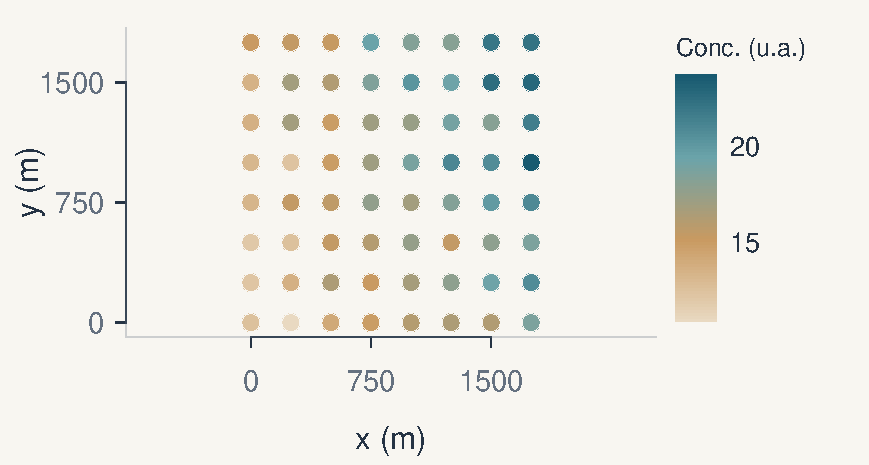
\includegraphics[width=9.85cm,height=5.25cm,keepaspectratio]{Risultati/Figure/01_mappa_punti.pdf}
\vspace{1.5mm}
\PSmall{64 siti della griglia locale. Stessa scala metrica sui due assi; colore = concentrazione in u.a.}

\end{minipage}\end{lrbox}
\typeout{FULLBOX:007:PilotLeftBox:\the\ht\PilotLeftBox:\the\dp\PilotLeftBox}

\begin{lrbox}{\PilotRightBox}
\begin{minipage}[t]{7.55cm}\raggedright\color{Ink}\fontsize{11.3}{14.8}\selectfont
\PBody{I simboli rappresentano campioni. Tra due simboli non è stata osservata una misura aggiuntiva.}
\vspace{2.5mm}
\PInfo{Una griglia regolare facilita il controllo dei passaggi. Non implica che il fenomeno naturale sia regolare o che ogni cella abbia lo stesso valore.}
\PBody{Prima di interpolare controlliamo estensione, punti mancanti, duplicati e leggibilità della scala cromatica.}
\vspace{2.5mm}

\end{minipage}\end{lrbox}
\typeout{FULLBOX:007:PilotRightBox:\the\ht\PilotRightBox:\the\dp\PilotRightBox}

\begin{tikzpicture}[remember picture,overlay]
\PilotChrome{La carta iniziale mostra ciò che osserviamo}{I · DATO E SUPPORTO}{7}{Una carta di punti deve rendere visibili i campioni e la copertura, prima di suggerire continuità.}
\node[anchor=north west,inner sep=0] at([xshift=.96cm,yshift=-2.13cm]current page.north west){\usebox{\PilotLeftBox}};
\node[anchor=north west,inner sep=0] at([xshift=11.52cm,yshift=-2.13cm]current page.north west){\usebox{\PilotRightBox}};
\node[anchor=north east,inner sep=0] at([xshift=17.65cm,yshift=-12.06cm]current page.north west){\color{Classical}\fontsize{7.7}{9.2}\selectfont\href{../../03_Notebook_svolti/M11_Locus/M11_N07.html}{M11\_N07 · notebook svolto}};
\end{tikzpicture}\end{frame}

\begin{frame}[plain]\hypertarget{slide8}{}
\bookmark[level=1,page=8]{La distribuzione marginale non conserva i luoghi}
\begin{lrbox}{\TitleBox}
\begin{minipage}[t]{17.7cm}\raggedright\color{Ink}\fontsize{11.3}{14.8}\selectfont
\color{Navy}\bfseries\fontsize{20.6}{24.5}\selectfont La distribuzione marginale non conserva i luoghi
\end{minipage}\end{lrbox}
\typeout{FULLBOX:008:TitleBox:\the\ht\TitleBox:\the\dp\TitleBox}

\begin{lrbox}{\RecallBox}
\begin{minipage}[t]{14.3cm}\raggedright\color{Ink}\fontsize{11.3}{14.8}\selectfont
\fontsize{10.3}{13.8}\selectfont La relazione tra valori e posizioni contiene informazione che l’istogramma non descrive.
\end{minipage}\end{lrbox}
\typeout{FULLBOX:008:RecallBox:\the\ht\RecallBox:\the\dp\RecallBox}

\begin{lrbox}{\PilotLeftBox}
\begin{minipage}[t]{10.05cm}\raggedright\color{Ink}\fontsize{11.3}{14.8}\selectfont
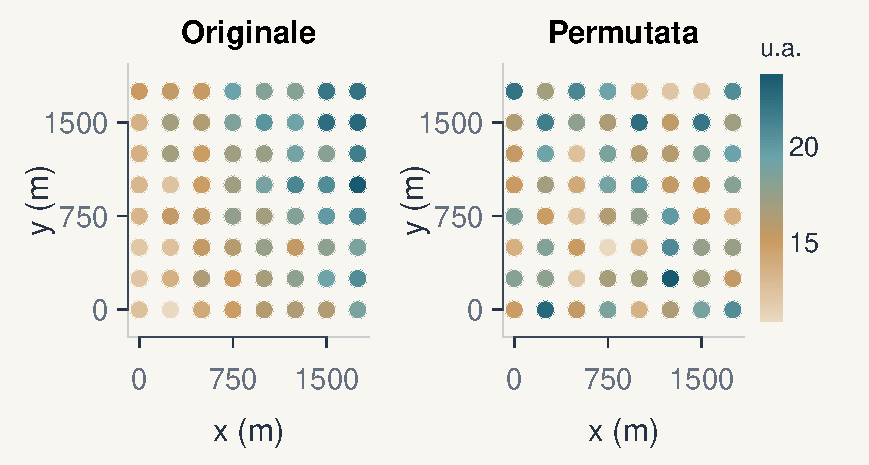
\includegraphics[width=9.85cm,height=5.25cm,keepaspectratio]{Risultati/Figure/02_marginale_permutata.pdf}
\vspace{1.5mm}
\PSmall{Gli stessi valori possono essere disposti diversamente. L’istogramma resta invariato.}

\end{minipage}\end{lrbox}
\typeout{FULLBOX:008:PilotLeftBox:\the\ht\PilotLeftBox:\the\dp\PilotLeftBox}

\begin{lrbox}{\PilotRightBox}
\begin{minipage}[t]{7.55cm}\raggedright\color{Ink}\fontsize{11.3}{14.8}\selectfont
\PBody{La permutazione conserva media, quantili e varianza. Cambia l’accoppiamento dei valori con le posizioni.}
\vspace{2.5mm}
\PInfo{Due carte con lo stesso istogramma possono avere concentrazioni simili raccolte in gruppi oppure alternate fra vicini.}
\PBody{L’analisi spaziale usa l’informazione congiunta di valori e luoghi.}
\vspace{2.5mm}
\PCode{R · stessi valori, altri luoghi}{008_esempio.R}
\end{minipage}\end{lrbox}
\typeout{FULLBOX:008:PilotRightBox:\the\ht\PilotRightBox:\the\dp\PilotRightBox}

\begin{tikzpicture}[remember picture,overlay]
\PilotChrome{La distribuzione marginale non conserva i luoghi}{I · DATO E SUPPORTO}{8}{La relazione tra valori e posizioni contiene informazione che l’istogramma non descrive.}
\node[anchor=north west,inner sep=0] at([xshift=.96cm,yshift=-2.13cm]current page.north west){\usebox{\PilotLeftBox}};
\node[anchor=north west,inner sep=0] at([xshift=11.52cm,yshift=-2.13cm]current page.north west){\usebox{\PilotRightBox}};
\end{tikzpicture}\end{frame}

\begin{frame}[plain]\hypertarget{slide9}{}
\bookmark[level=1,page=9]{Un punto e una media areale hanno supporti diversi}
\begin{lrbox}{\TitleBox}
\begin{minipage}[t]{17.7cm}\raggedright\color{Ink}\fontsize{11.3}{14.8}\selectfont
\color{Navy}\bfseries\fontsize{20.6}{24.5}\selectfont Un punto e una media areale hanno supporti diversi
\end{minipage}\end{lrbox}
\typeout{FULLBOX:009:TitleBox:\the\ht\TitleBox:\the\dp\TitleBox}

\begin{lrbox}{\RecallBox}
\begin{minipage}[t]{14.3cm}\raggedright\color{Ink}\fontsize{11.3}{14.8}\selectfont
\fontsize{10.3}{13.8}\selectfont Il supporto appartiene alla definizione della variabile e deve accompagnare ogni confronto.
\end{minipage}\end{lrbox}
\typeout{FULLBOX:009:RecallBox:\the\ht\RecallBox:\the\dp\RecallBox}

\begin{lrbox}{\PilotLeftBox}
\begin{minipage}[t]{10.05cm}\raggedright\color{Ink}\fontsize{11.3}{14.8}\selectfont
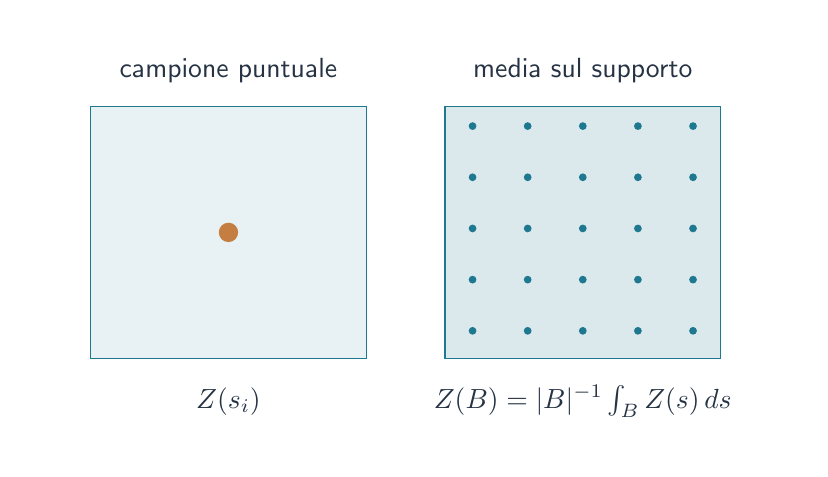
\begin{tikzpicture}[x=1cm,y=1cm]
\path[use as bounding box](-.1,-.15) rectangle(9.7,5.2);
\filldraw[fill=GeoA!10,draw=GeoA](.7,1.0)rectangle(4.2,4.2);
\fill[GeoB](2.45,2.6)circle(3.5pt);
\node[pLabel]at(2.45,4.65){campione puntuale};
\node[pLabel]at(2.45,.45){$Z(s_i)$};
\filldraw[fill=GeoA!16,draw=GeoA](5.2,1.0)rectangle(8.7,4.2);
\foreach \x in {5.55,6.25,6.95,7.65,8.35}
 \foreach \y in {1.35,2.0,2.65,3.3,3.95}{\fill[GeoA](\x,\y)circle(1.4pt);}
\node[pLabel]at(6.95,4.65){media sul supporto};
\node[pLabel]at(6.95,.45){$Z(B)=|B|^{-1}\int_B Z(s)\,ds$};
\end{tikzpicture}

\end{minipage}\end{lrbox}
\typeout{FULLBOX:009:PilotLeftBox:\the\ht\PilotLeftBox:\the\dp\PilotLeftBox}

\begin{lrbox}{\PilotRightBox}
\begin{minipage}[t]{7.55cm}\raggedright\color{Ink}\fontsize{11.3}{14.8}\selectfont
\PBody{Il dato puntuale approssima la misura in una posizione. Il dato areale riassume una regione; richiede una definizione della media sul supporto.}
\vspace{2.5mm}
\PInfo{Un simbolo al centro di un poligono può rappresentare la media del poligono. Il punto disegnato non trasforma quella media in una misura puntuale.}
\PBody{Prima di confrontare osservazioni provenienti da strumenti diversi, verifichiamo se misurano lo stesso supporto.}
\vspace{2.5mm}

\end{minipage}\end{lrbox}
\typeout{FULLBOX:009:PilotRightBox:\the\ht\PilotRightBox:\the\dp\PilotRightBox}

\begin{tikzpicture}[remember picture,overlay]
\PilotChrome{Un punto e una media areale hanno supporti diversi}{I · DATO E SUPPORTO}{9}{Il supporto appartiene alla definizione della variabile e deve accompagnare ogni confronto.}
\node[anchor=north west,inner sep=0] at([xshift=.96cm,yshift=-2.13cm]current page.north west){\usebox{\PilotLeftBox}};
\node[anchor=north west,inner sep=0] at([xshift=11.52cm,yshift=-2.13cm]current page.north west){\usebox{\PilotRightBox}};
\end{tikzpicture}\end{frame}

\begin{frame}[plain]\hypertarget{slide10}{}
\bookmark[level=1,page=10]{Cambiare supporto cambia la quantità studiata}
\begin{lrbox}{\TitleBox}
\begin{minipage}[t]{17.7cm}\raggedright\color{Ink}\fontsize{11.3}{14.8}\selectfont
\color{Navy}\bfseries\fontsize{20.6}{24.5}\selectfont Cambiare supporto cambia la quantità studiata
\end{minipage}\end{lrbox}
\typeout{FULLBOX:010:TitleBox:\the\ht\TitleBox:\the\dp\TitleBox}

\begin{lrbox}{\RecallBox}
\begin{minipage}[t]{14.3cm}\raggedright\color{Ink}\fontsize{11.3}{14.8}\selectfont
\fontsize{10.3}{13.8}\selectfont La scala del supporto entra sia nella media sia nella sua variabilità.
\end{minipage}\end{lrbox}
\typeout{FULLBOX:010:RecallBox:\the\ht\RecallBox:\the\dp\RecallBox}

\begin{lrbox}{\PilotLeftBox}
\begin{minipage}[t]{10.05cm}\raggedright\color{Ink}\fontsize{11.3}{14.8}\selectfont
\[Z(B)=\frac{1}{|B|}\int_B Z(s)\,ds\]
\[\operatorname{Var}\{Z(B)\}=\frac{1}{|B|^2}\int_B\int_B C(s,t)\,ds\,dt\]
\PInfo{La seconda relazione assume una covarianza integrabile. La variabilità della media dipende dalla forma del supporto e dalla covarianza tra le posizioni.}

\end{minipage}\end{lrbox}
\typeout{FULLBOX:010:PilotLeftBox:\the\ht\PilotLeftBox:\the\dp\PilotLeftBox}

\begin{lrbox}{\PilotRightBox}
\begin{minipage}[t]{7.55cm}\raggedright\color{Ink}\fontsize{11.3}{14.8}\selectfont
\PBody{Una media su un’area non coincide automaticamente con il valore nel suo centro. Per stimarla da campioni occorre considerare come quei campioni coprono l’area.}
\vspace{2.5mm}
\PBody{L’aggregazione spesso attenua le oscillazioni, ma l’effetto quantitativo dipende dalla struttura del processo e dal supporto.}
\vspace{2.5mm}
\PSmall{Nel modulo distinguiamo medie dei siti osservati e medie territoriali. Non attribuiamo loro lo stesso significato senza un disegno di campionamento.}

\end{minipage}\end{lrbox}
\typeout{FULLBOX:010:PilotRightBox:\the\ht\PilotRightBox:\the\dp\PilotRightBox}

\begin{tikzpicture}[remember picture,overlay]
\PilotChrome{Cambiare supporto cambia la quantità studiata}{I · DATO E SUPPORTO}{10}{La scala del supporto entra sia nella media sia nella sua variabilità.}
\node[anchor=north west,inner sep=0] at([xshift=.96cm,yshift=-2.13cm]current page.north west){\usebox{\PilotLeftBox}};
\node[anchor=north west,inner sep=0] at([xshift=11.52cm,yshift=-2.13cm]current page.north west){\usebox{\PilotRightBox}};
\end{tikzpicture}\end{frame}

\begin{frame}[plain]\hypertarget{slide11}{}
\bookmark[level=1,page=11]{Dai siti ai blocchi: esplicitare i pesi}
\begin{lrbox}{\TitleBox}
\begin{minipage}[t]{17.7cm}\raggedright\color{Ink}\fontsize{11.3}{14.8}\selectfont
\color{Navy}\bfseries\fontsize{20.6}{24.5}\selectfont Dai siti ai blocchi: esplicitare i pesi
\end{minipage}\end{lrbox}
\typeout{FULLBOX:011:TitleBox:\the\ht\TitleBox:\the\dp\TitleBox}

\begin{lrbox}{\RecallBox}
\begin{minipage}[t]{14.3cm}\raggedright\color{Ink}\fontsize{11.3}{14.8}\selectfont
\fontsize{10.3}{13.8}\selectfont La coincidenza tra due medie può dipendere dal bilanciamento del disegno, non da un’identità generale.
\end{minipage}\end{lrbox}
\typeout{FULLBOX:011:RecallBox:\the\ht\RecallBox:\the\dp\RecallBox}

\begin{lrbox}{\FullWideBox}
\begin{minipage}[t]{18.1cm}\raggedright\color{Ink}\fontsize{11.3}{14.8}\selectfont
\centering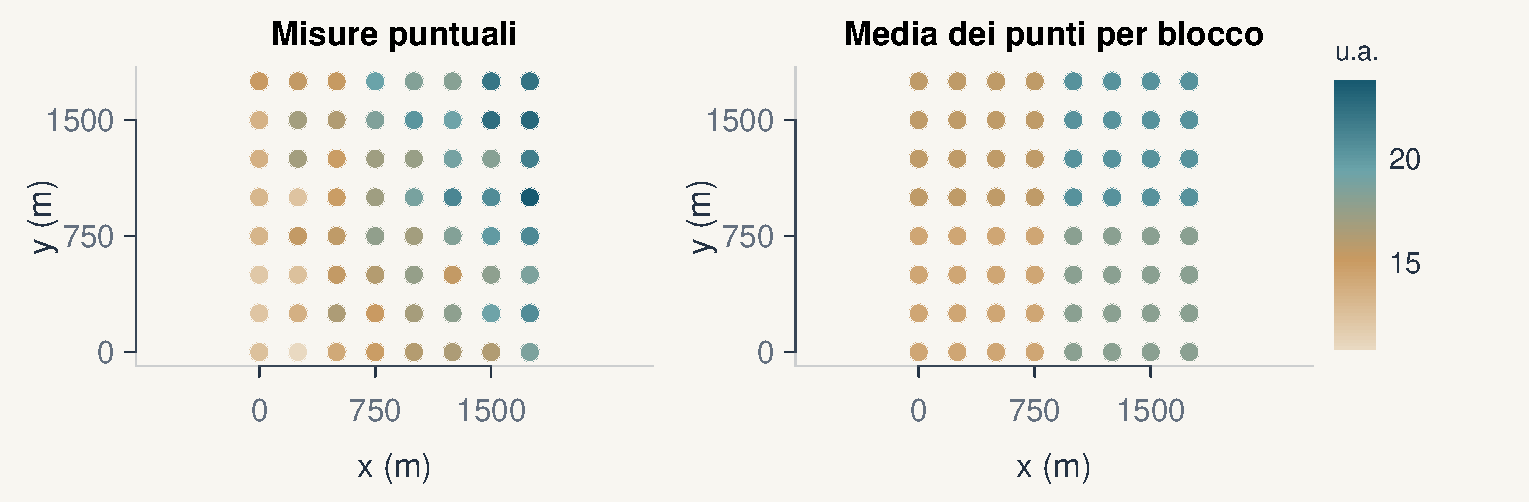
\includegraphics[width=18.05cm,height=5.8cm,keepaspectratio]{Risultati/Figure/03_supporto_blocchi.pdf}
\end{minipage}\end{lrbox}
\typeout{FULLBOX:011:FullWideBox:\the\ht\FullWideBox:\the\dp\FullWideBox}

\begin{lrbox}{\PilotRightBox}
\begin{minipage}[t]{18.1cm}\raggedright\color{Ink}\fontsize{11.3}{14.8}\selectfont
\PBody{Quattro blocchi, 16 siti ciascuno. La media dei siti pesa ogni osservazione allo stesso modo; la media semplice dei blocchi pesa ogni blocco allo stesso modo. Qui coincidono perché le numerosità sono uguali. Per interpretare una media come areale servono pesi coerenti con le aree rappresentate o con il disegno.}
\end{minipage}\end{lrbox}
\typeout{FULLBOX:011:PilotRightBox:\the\ht\PilotRightBox:\the\dp\PilotRightBox}

\begin{tikzpicture}[remember picture,overlay]
\PilotChrome{Dai siti ai blocchi: esplicitare i pesi}{I · DATO E SUPPORTO}{11}{La coincidenza tra due medie può dipendere dal bilanciamento del disegno, non da un’identità generale.}
\node[anchor=north west,inner sep=0] at([xshift=.96cm,yshift=-2.13cm]current page.north west){\usebox{\FullWideBox}};
\node[anchor=north west,inner sep=0] at([xshift=.96cm,yshift=-8.25cm]current page.north west){\usebox{\PilotRightBox}};
\node[anchor=north east,inner sep=0] at([xshift=17.65cm,yshift=-12.06cm]current page.north west){\color{Classical}\fontsize{7.7}{9.2}\selectfont\href{../../03_Notebook_svolti/M11_Locus/M11_N17.html}{M11\_N17 · notebook svolto}};
\end{tikzpicture}\end{frame}

\begin{frame}[plain]\hypertarget{slide12}{}
\bookmark[level=1,page=12]{Repliche nello stesso luogo e nuovi siti}
\begin{lrbox}{\TitleBox}
\begin{minipage}[t]{17.7cm}\raggedright\color{Ink}\fontsize{11.3}{14.8}\selectfont
\color{Navy}\bfseries\fontsize{20.6}{24.5}\selectfont Repliche nello stesso luogo e nuovi siti
\end{minipage}\end{lrbox}
\typeout{FULLBOX:012:TitleBox:\the\ht\TitleBox:\the\dp\TitleBox}

\begin{lrbox}{\RecallBox}
\begin{minipage}[t]{14.3cm}\raggedright\color{Ink}\fontsize{11.3}{14.8}\selectfont
\fontsize{10.3}{13.8}\selectfont Nuove righe e nuove unità campionate sono concetti da verificare separatamente.
\end{minipage}\end{lrbox}
\typeout{FULLBOX:012:RecallBox:\the\ht\RecallBox:\the\dp\RecallBox}

\begin{lrbox}{\PilotLeftBox}
\begin{minipage}[t]{10.05cm}\raggedright\color{Ink}\fontsize{11.3}{14.8}\selectfont
{\fontsize{10.2}{13.1}\selectfont\renewcommand{\arraystretch}{1.45}\begin{tabular}{@{}p{4.2cm}p{4.8cm}@{}}\toprule
\textbf{Operazione} & \textbf{Informazione aggiunta}\\\midrule
Ripetere una misura nello stesso sito & Ripetibilità della misura, a condizioni fissate\\
Campionare un luogo distante & Copertura di un’altra parte del dominio\\
Dividere una misura in più righe & Nessuna nuova osservazione indipendente\\
Aggregare più campioni & Nuovo supporto, perdita di dettaglio\\
\bottomrule\end{tabular}}

\end{minipage}\end{lrbox}
\typeout{FULLBOX:012:PilotLeftBox:\the\ht\PilotLeftBox:\the\dp\PilotLeftBox}

\begin{lrbox}{\PilotRightBox}
\begin{minipage}[t]{7.55cm}\raggedright\color{Ink}\fontsize{11.3}{14.8}\selectfont
\PBody{La numerosità delle righe non misura da sola l’informazione spaziale. Occorre sapere se i dati provengono da nuovi luoghi o da ripetizioni della stessa unità.}
\vspace{2.5mm}
\PInfo{I duplicati possono essere errori, repliche vere oppure esiti di un join con più appartenenze. Il trattamento dipende dal motivo della duplicazione.}
\PBody{Non eliminiamo righe automaticamente prima di aver chiarito che cosa rappresentano.}
\vspace{2.5mm}

\end{minipage}\end{lrbox}
\typeout{FULLBOX:012:PilotRightBox:\the\ht\PilotRightBox:\the\dp\PilotRightBox}

\begin{tikzpicture}[remember picture,overlay]
\PilotChrome{Repliche nello stesso luogo e nuovi siti}{I · DATO E SUPPORTO}{12}{Nuove righe e nuove unità campionate sono concetti da verificare separatamente.}
\node[anchor=north west,inner sep=0] at([xshift=.96cm,yshift=-2.13cm]current page.north west){\usebox{\PilotLeftBox}};
\node[anchor=north west,inner sep=0] at([xshift=11.52cm,yshift=-2.13cm]current page.north west){\usebox{\PilotRightBox}};
\end{tikzpicture}\end{frame}

\begin{frame}[plain]\hypertarget{slide13}{}
\bookmark[level=1,page=13]{L’identificativo protegge l’allineamento}
\begin{lrbox}{\TitleBox}
\begin{minipage}[t]{17.7cm}\raggedright\color{Ink}\fontsize{11.3}{14.8}\selectfont
\color{Navy}\bfseries\fontsize{20.6}{24.5}\selectfont L’identificativo protegge l’allineamento
\end{minipage}\end{lrbox}
\typeout{FULLBOX:013:TitleBox:\the\ht\TitleBox:\the\dp\TitleBox}

\begin{lrbox}{\RecallBox}
\begin{minipage}[t]{14.3cm}\raggedright\color{Ink}\fontsize{11.3}{14.8}\selectfont
\fontsize{10.3}{13.8}\selectfont L’allineamento per identificativo è parte della correttezza del calcolo spaziale.
\end{minipage}\end{lrbox}
\typeout{FULLBOX:013:RecallBox:\the\ht\RecallBox:\the\dp\RecallBox}

\begin{lrbox}{\PilotLeftBox}
\begin{minipage}[t]{10.05cm}\raggedright\color{Ink}\fontsize{11.3}{14.8}\selectfont
\[z_i\longleftrightarrow s_i\longleftrightarrow W_{i\cdot}\]
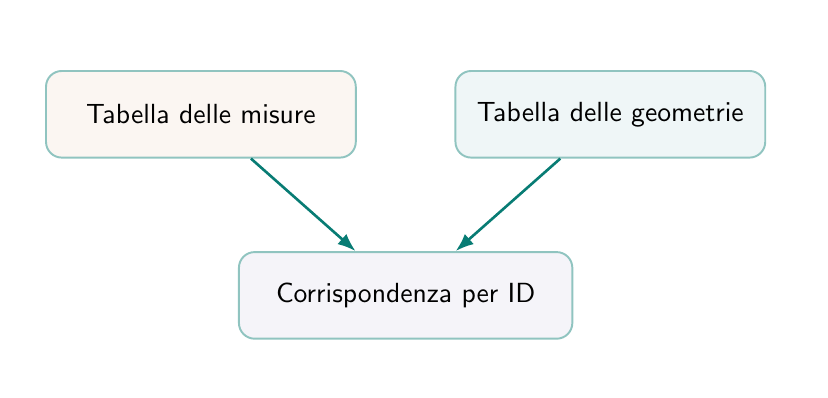
\begin{tikzpicture}[x=1cm,y=1cm]
\path[use as bounding box](-.1,-.15) rectangle(9.7,4.2);
\node[pFlow,text width=3.7cm,fill=GeoB!7] (a) at(2.1,3.1){Tabella delle misure};
\node[pFlow,text width=3.7cm,fill=GeoA!7] (b) at(7.3,3.1){Tabella delle geometrie};
\node[pFlow,text width=4.0cm,fill=GeoC!7] (c) at(4.7,0.8){Corrispondenza per ID};
\draw[pEdge] (a) -- (c);
\draw[pEdge] (b) -- (c);
\end{tikzpicture}

\end{minipage}\end{lrbox}
\typeout{FULLBOX:013:PilotLeftBox:\the\ht\PilotLeftBox:\the\dp\PilotLeftBox}

\begin{lrbox}{\PilotRightBox}
\begin{minipage}[t]{7.55cm}\raggedright\color{Ink}\fontsize{11.3}{14.8}\selectfont
\PBody{Le distanze e i pesi dipendono dall’ordine delle coordinate. Il vettore delle misure deve seguire esattamente lo stesso ordine.}
\vspace{2.5mm}
\PInfo{Una matrice quadrata della dimensione giusta può essere associata ai valori sbagliati. Il controllo delle dimensioni non basta.}
\PCode{R · legare righe e geometria}{013_esempio.R}
\end{minipage}\end{lrbox}
\typeout{FULLBOX:013:PilotRightBox:\the\ht\PilotRightBox:\the\dp\PilotRightBox}

\begin{tikzpicture}[remember picture,overlay]
\PilotChrome{L’identificativo protegge l’allineamento}{I · DATO E SUPPORTO}{13}{L’allineamento per identificativo è parte della correttezza del calcolo spaziale.}
\node[anchor=north west,inner sep=0] at([xshift=.96cm,yshift=-2.13cm]current page.north west){\usebox{\PilotLeftBox}};
\node[anchor=north west,inner sep=0] at([xshift=11.52cm,yshift=-2.13cm]current page.north west){\usebox{\PilotRightBox}};
\node[anchor=north east,inner sep=0] at([xshift=17.65cm,yshift=-12.06cm]current page.north west){\color{Classical}\fontsize{7.7}{9.2}\selectfont\href{../../03_Notebook_svolti/M11_Locus/M11_N01.html}{M11\_N01 · notebook svolto}};
\end{tikzpicture}\end{frame}

\begin{frame}[plain]\hypertarget{slide14}{}
\bookmark[level=1,page=14]{L’audit precede ogni trasformazione}
\begin{lrbox}{\TitleBox}
\begin{minipage}[t]{17.7cm}\raggedright\color{Ink}\fontsize{11.3}{14.8}\selectfont
\color{Navy}\bfseries\fontsize{20.6}{24.5}\selectfont L’audit precede ogni trasformazione
\end{minipage}\end{lrbox}
\typeout{FULLBOX:014:TitleBox:\the\ht\TitleBox:\the\dp\TitleBox}

\begin{lrbox}{\RecallBox}
\begin{minipage}[t]{14.3cm}\raggedright\color{Ink}\fontsize{11.3}{14.8}\selectfont
\fontsize{10.3}{13.8}\selectfont Controlli semplici eseguiti all’ingresso impediscono che un errore di coordinate attraversi l’intera analisi.
\end{minipage}\end{lrbox}
\typeout{FULLBOX:014:RecallBox:\the\ht\RecallBox:\the\dp\RecallBox}

\begin{lrbox}{\PilotLeftBox}
\begin{minipage}[t]{10.05cm}\raggedright\color{Ink}\fontsize{11.3}{14.8}\selectfont
{\fontsize{10.2}{13.1}\selectfont\renewcommand{\arraystretch}{1.45}\begin{tabular}{@{}p{3.2cm}p{5.8cm}@{}}\toprule
\textbf{Controllo} & \textbf{Criterio nel caso guida}\\\midrule
Identità & 64 ID distinti, nessun ID mancante\\
Coordinate & Valori numerici e finiti\\
Estensione locale & 0--1750 m per asse\\
Griglia & 8 valori distinti per asse\\
Variabile & 64 concentrazioni finite\\
Metadati & Unità e origine dichiarate\\
\bottomrule\end{tabular}}

\end{minipage}\end{lrbox}
\typeout{FULLBOX:014:PilotLeftBox:\the\ht\PilotLeftBox:\the\dp\PilotLeftBox}

\begin{lrbox}{\PilotRightBox}
\begin{minipage}[t]{7.55cm}\raggedright\color{Ink}\fontsize{11.3}{14.8}\selectfont
\PBody{Un audit combina controlli automatici e conoscenza del contesto. Il programma riconosce molti errori di formato; non può ricostruire da solo un CRS ignoto.}
\vspace{2.5mm}
\PInfo{Il notebook N01 salva un riepilogo dei campi. I controlli trasformano assunzioni del caso didattico in condizioni verificabili.}
\PCode{R · audit minimo}{014_esempio.R}
\end{minipage}\end{lrbox}
\typeout{FULLBOX:014:PilotRightBox:\the\ht\PilotRightBox:\the\dp\PilotRightBox}

\begin{tikzpicture}[remember picture,overlay]
\PilotChrome{L’audit precede ogni trasformazione}{I · DATO E SUPPORTO}{14}{Controlli semplici eseguiti all’ingresso impediscono che un errore di coordinate attraversi l’intera analisi.}
\node[anchor=north west,inner sep=0] at([xshift=.96cm,yshift=-2.13cm]current page.north west){\usebox{\PilotLeftBox}};
\node[anchor=north west,inner sep=0] at([xshift=11.52cm,yshift=-2.13cm]current page.north west){\usebox{\PilotRightBox}};
\node[anchor=north east,inner sep=0] at([xshift=17.65cm,yshift=-12.06cm]current page.north west){\color{Classical}\fontsize{7.7}{9.2}\selectfont\href{../../03_Notebook_svolti/M11_Locus/M11_N01.html}{M11\_N01 · notebook svolto}};
\end{tikzpicture}\end{frame}

\begin{frame}[plain]\hypertarget{slide15}{}
\bookmark[level=1,page=15]{Due rappresentazioni con origini distinte}
\begin{lrbox}{\TitleBox}
\begin{minipage}[t]{17.7cm}\raggedright\color{Ink}\fontsize{11.3}{14.8}\selectfont
\color{Navy}\bfseries\fontsize{20.6}{24.5}\selectfont Due rappresentazioni con origini distinte
\end{minipage}\end{lrbox}
\typeout{FULLBOX:015:TitleBox:\the\ht\TitleBox:\the\dp\TitleBox}

\begin{lrbox}{\RecallBox}
\begin{minipage}[t]{14.3cm}\raggedright\color{Ink}\fontsize{11.3}{14.8}\selectfont
\fontsize{10.3}{13.8}\selectfont Coordinate espresse in metri possono appartenere a sistemi diversi e non essere intercambiabili.
\end{minipage}\end{lrbox}
\typeout{FULLBOX:015:RecallBox:\the\ht\RecallBox:\the\dp\RecallBox}

\begin{lrbox}{\PilotLeftBox}
\begin{minipage}[t]{10.05cm}\raggedright\color{Ink}\fontsize{11.3}{14.8}\selectfont
{\fontsize{10.2}{13.1}\selectfont\renewcommand{\arraystretch}{1.45}\begin{tabular}{@{}p{4.5cm}p{4.5cm}@{}}\toprule
\textbf{Coordinate locali} & \textbf{Coordinate geografiche}\\\midrule
$x,y$ in metri & Longitudine, latitudine in gradi\\
Origine convenzionale & Collocazione sintetica vicino a 9° E, 45° N\\
Distanza euclidea del laboratorio & Proiezioni e distanze sulla Terra\\
Nessun EPSG dedotto dai numeri & CRS geografico dichiarato nell’esercizio\\
\bottomrule\end{tabular}}

\end{minipage}\end{lrbox}
\typeout{FULLBOX:015:PilotLeftBox:\the\ht\PilotLeftBox:\the\dp\PilotLeftBox}

\begin{lrbox}{\PilotRightBox}
\begin{minipage}[t]{7.55cm}\raggedright\color{Ink}\fontsize{11.3}{14.8}\selectfont
\PBody{Il dataset contiene due rappresentazioni didattiche. Le coordinate geografiche derivano da una collocazione sintetica approssimata della griglia.}
\vspace{2.5mm}
\PInfo{Proiettare longitudine e latitudine produce coordinate UTM. Non ricostruisce esattamente le colonne locali per semplice sottrazione di un’origine.}
\PBody{Conserveremo le colonne originali e indicheremo in ogni figura quale sistema è stato usato.}
\vspace{2.5mm}

\end{minipage}\end{lrbox}
\typeout{FULLBOX:015:PilotRightBox:\the\ht\PilotRightBox:\the\dp\PilotRightBox}

\begin{tikzpicture}[remember picture,overlay]
\PilotChrome{Due rappresentazioni con origini distinte}{I · DATO E SUPPORTO}{15}{Coordinate espresse in metri possono appartenere a sistemi diversi e non essere intercambiabili.}
\node[anchor=north west,inner sep=0] at([xshift=.96cm,yshift=-2.13cm]current page.north west){\usebox{\PilotLeftBox}};
\node[anchor=north west,inner sep=0] at([xshift=11.52cm,yshift=-2.13cm]current page.north west){\usebox{\PilotRightBox}};
\node[anchor=north east,inner sep=0] at([xshift=17.65cm,yshift=-12.06cm]current page.north west){\color{Classical}\fontsize{7.7}{9.2}\selectfont\href{../../03_Notebook_svolti/M11_Locus/M11_N05.html}{M11\_N05 · notebook svolto}};
\end{tikzpicture}\end{frame}

\begin{frame}[plain]\hypertarget{slide16}{}
\bookmark[level=1,page=16]{Primo laboratorio: descrivere il dato}
\begin{lrbox}{\TitleBox}
\begin{minipage}[t]{17.7cm}\raggedright\color{Ink}\fontsize{11.3}{14.8}\selectfont
\color{Navy}\bfseries\fontsize{20.6}{24.5}\selectfont Primo laboratorio: descrivere il dato
\end{minipage}\end{lrbox}
\typeout{FULLBOX:016:TitleBox:\the\ht\TitleBox:\the\dp\TitleBox}

\begin{lrbox}{\RecallBox}
\begin{minipage}[t]{14.3cm}\raggedright\color{Ink}\fontsize{11.3}{14.8}\selectfont
\fontsize{10.3}{13.8}\selectfont Un’analisi spaziale comincia con una descrizione verificabile dell’unità osservata.
\end{minipage}\end{lrbox}
\typeout{FULLBOX:016:RecallBox:\the\ht\RecallBox:\the\dp\RecallBox}

\begin{lrbox}{\PilotLeftBox}
\begin{minipage}[t]{10.05cm}\raggedright\color{Ink}\fontsize{11.3}{14.8}\selectfont
\PLab{https://marzione00.github.io/Lab_Geo/\#laboratorio/m11-supporto}{Esperimento online · dato e supporto}
{\fontsize{10.2}{13.1}\selectfont\renewcommand{\arraystretch}{1.45}\begin{tabular}{@{}p{3.7cm}p{5.3cm}@{}}\toprule
\textbf{Consegna} & \textbf{Evidenza richiesta}\\\midrule
Una tabella documentata & ID, unità, supporto e provenienza\\
Una carta di punti & Assi, scala cromatica, siti visibili\\
Un controllo di integrità & Conteggi e valori mancanti\\
Una domanda scientifica & Quantità da descrivere o prevedere\\
\bottomrule\end{tabular}}

\end{minipage}\end{lrbox}
\typeout{FULLBOX:016:PilotLeftBox:\the\ht\PilotLeftBox:\the\dp\PilotLeftBox}

\begin{lrbox}{\PilotRightBox}
\begin{minipage}[t]{7.55cm}\raggedright\color{Ink}\fontsize{11.3}{14.8}\selectfont
\PBody{N01 verifica la tabella; N07 costruisce la carta iniziale. N17 tornerà sulla distinzione tra medie dei siti e medie dei blocchi.}
\vspace{2.5mm}
\PInfo{Prima di procedere, spiegare a parole che cosa rappresenta ogni punto. Se la risposta cambia dopo un’aggregazione, deve cambiare anche la descrizione del risultato.}
\PBody{Il fascicolo passa ora dai luoghi come metadati ai luoghi come oggetti su cui calcolare distanze.}
\vspace{2.5mm}

\end{minipage}\end{lrbox}
\typeout{FULLBOX:016:PilotRightBox:\the\ht\PilotRightBox:\the\dp\PilotRightBox}

\begin{tikzpicture}[remember picture,overlay]
\PilotChrome{Primo laboratorio: descrivere il dato}{I · DATO E SUPPORTO}{16}{Un’analisi spaziale comincia con una descrizione verificabile dell’unità osservata.}
\node[anchor=north west,inner sep=0] at([xshift=.96cm,yshift=-2.13cm]current page.north west){\usebox{\PilotLeftBox}};
\node[anchor=north west,inner sep=0] at([xshift=11.52cm,yshift=-2.13cm]current page.north west){\usebox{\PilotRightBox}};
\node[anchor=north east,inner sep=0] at([xshift=17.65cm,yshift=-12.06cm]current page.north west){\color{Classical}\fontsize{7.7}{9.2}\selectfont\href{../../03_Notebook_svolti/M11_Locus/M11_N01.html}{M11\_N01 · notebook svolto}};
\end{tikzpicture}\end{frame}

\begin{frame}[plain]\hypertarget{slide17}{}
\bookmark[level=0,page=17]{II · COORDINATE E DISTANZE}
\bookmark[level=1,page=17]{I numeri delle coordinate richiedono una metrica}
\begin{lrbox}{\TitleBox}
\begin{minipage}[t]{17.7cm}\raggedright\color{Ink}\fontsize{11.3}{14.8}\selectfont
\color{Navy}\bfseries\fontsize{20.6}{24.5}\selectfont I numeri delle coordinate richiedono una metrica
\end{minipage}\end{lrbox}
\typeout{FULLBOX:017:TitleBox:\the\ht\TitleBox:\the\dp\TitleBox}

\begin{lrbox}{\RecallBox}
\begin{minipage}[t]{14.3cm}\raggedright\color{Ink}\fontsize{11.3}{14.8}\selectfont
\fontsize{10.3}{13.8}\selectfont La metrica traduce coordinate in distanze interpretabili.
\end{minipage}\end{lrbox}
\typeout{FULLBOX:017:RecallBox:\the\ht\RecallBox:\the\dp\RecallBox}

\begin{lrbox}{\PilotLeftBox}
\begin{minipage}[t]{10.05cm}\raggedright\color{Ink}\fontsize{11.3}{14.8}\selectfont
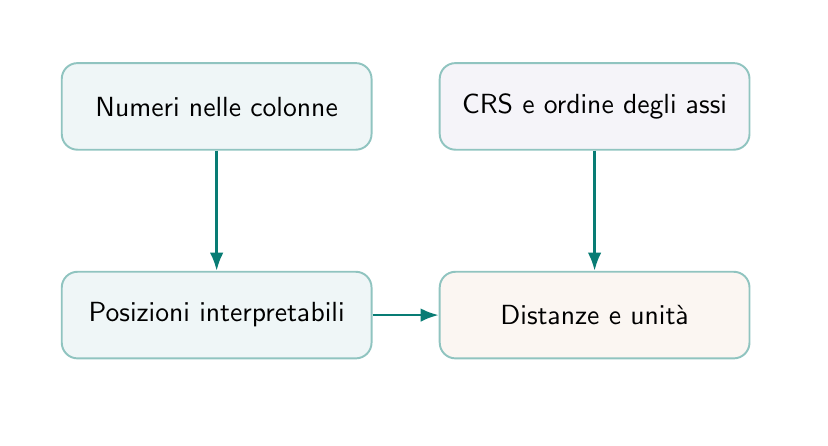
\begin{tikzpicture}[x=1cm,y=1cm]
\path[use as bounding box](-.1,-.15) rectangle(9.7,4.8);
\node[pFlow,text width=3.7cm,fill=GeoA!7] (a) at(2.3,3.8){Numeri nelle colonne};
\node[pFlow,text width=3.7cm,fill=GeoC!7] (b) at(7.1,3.8){CRS e ordine degli assi};
\node[pFlow,text width=3.7cm,fill=GeoA!7] (c) at(2.3,1.15){Posizioni interpretabili};
\node[pFlow,text width=3.7cm,fill=GeoB!7] (d) at(7.1,1.15){Distanze e unità};
\draw[pEdge] (a) -- (c);
\draw[pEdge] (b) -- (d);
\draw[pEdge] (c) -- (d);
\end{tikzpicture}

\end{minipage}\end{lrbox}
\typeout{FULLBOX:017:PilotLeftBox:\the\ht\PilotLeftBox:\the\dp\PilotLeftBox}

\begin{lrbox}{\PilotRightBox}
\begin{minipage}[t]{7.55cm}\raggedright\color{Ink}\fontsize{11.3}{14.8}\selectfont
\PBody{Un numero come 9 o 500000 non identifica un luogo senza sistema di riferimento e ordine degli assi. Anche l’unità deve essere nota.}
\vspace{2.5mm}
\PInfo{La distanza euclidea tra due colonne numeriche è sempre calcolabile. Il suo significato fisico dipende da ciò che rappresentano quelle colonne.}
\PBody{Per le operazioni locali usiamo metri nel piano. Per longitudine e latitudine dichiariamo la geometria terrestre adottata.}
\vspace{2.5mm}

\end{minipage}\end{lrbox}
\typeout{FULLBOX:017:PilotRightBox:\the\ht\PilotRightBox:\the\dp\PilotRightBox}

\begin{tikzpicture}[remember picture,overlay]
\PilotChrome{I numeri delle coordinate richiedono una metrica}{II · COORDINATE E DISTANZE}{17}{La metrica traduce coordinate in distanze interpretabili.}
\node[anchor=north west,inner sep=0] at([xshift=.96cm,yshift=-2.13cm]current page.north west){\usebox{\PilotLeftBox}};
\node[anchor=north west,inner sep=0] at([xshift=11.52cm,yshift=-2.13cm]current page.north west){\usebox{\PilotRightBox}};
\end{tikzpicture}\end{frame}

\begin{frame}[plain]\hypertarget{slide18}{}
\bookmark[level=1,page=18]{Invertire gli assi può superare i controlli globali}
\begin{lrbox}{\TitleBox}
\begin{minipage}[t]{17.7cm}\raggedright\color{Ink}\fontsize{11.3}{14.8}\selectfont
\color{Navy}\bfseries\fontsize{20.6}{24.5}\selectfont Invertire gli assi può superare i controlli globali
\end{minipage}\end{lrbox}
\typeout{FULLBOX:018:TitleBox:\the\ht\TitleBox:\the\dp\TitleBox}

\begin{lrbox}{\RecallBox}
\begin{minipage}[t]{14.3cm}\raggedright\color{Ink}\fontsize{11.3}{14.8}\selectfont
\fontsize{10.3}{13.8}\selectfont Un valore plausibile per intervallo può essere sbagliato per posizione.
\end{minipage}\end{lrbox}
\typeout{FULLBOX:018:RecallBox:\the\ht\RecallBox:\the\dp\RecallBox}

\begin{lrbox}{\PilotLeftBox}
\begin{minipage}[t]{10.05cm}\raggedright\color{Ink}\fontsize{11.3}{14.8}\selectfont
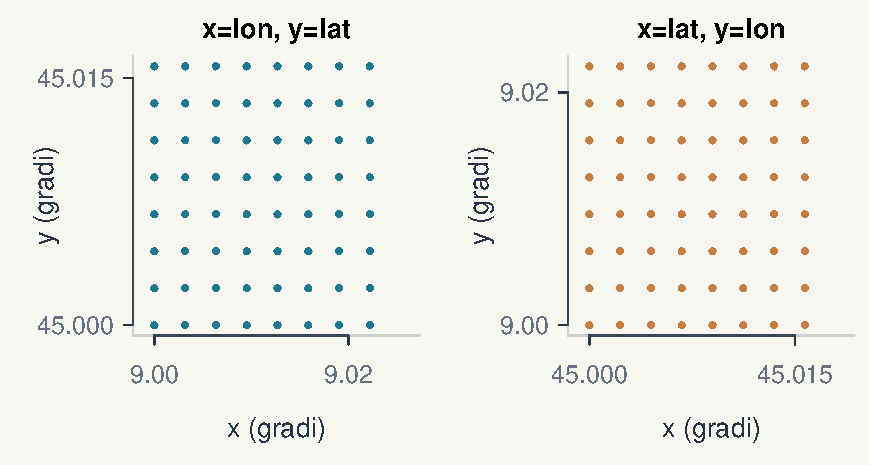
\includegraphics[width=9.85cm,height=5.25cm,keepaspectratio]{Risultati/Figure/04_coordinate_invertite.pdf}
\vspace{1.5mm}
\PSmall{Le coppie (9°,45°) e (45°,9°) rispettano entrambe i limiti globali, ma indicano luoghi diversi.}

\end{minipage}\end{lrbox}
\typeout{FULLBOX:018:PilotLeftBox:\the\ht\PilotLeftBox:\the\dp\PilotLeftBox}

\begin{lrbox}{\PilotRightBox}
\begin{minipage}[t]{7.55cm}\raggedright\color{Ink}\fontsize{11.3}{14.8}\selectfont
\PBody{La longitudine deve trovarsi tra $-180^\circ$ e $180^\circ$; la latitudine tra $-90^\circ$ e $90^\circ$. Sono condizioni necessarie, non una prova dell’ordine corretto.}
\vspace{2.5mm}
\PInfo{Nel caso guida servono anche un’area attesa e metadati affidabili. Scambiare le colonne può spostare i punti senza generare un errore numerico.}
\PCode{R · limiti necessari, non sufficienti}{018_esempio.R}
\end{minipage}\end{lrbox}
\typeout{FULLBOX:018:PilotRightBox:\the\ht\PilotRightBox:\the\dp\PilotRightBox}

\begin{tikzpicture}[remember picture,overlay]
\PilotChrome{Invertire gli assi può superare i controlli globali}{II · COORDINATE E DISTANZE}{18}{Un valore plausibile per intervallo può essere sbagliato per posizione.}
\node[anchor=north west,inner sep=0] at([xshift=.96cm,yshift=-2.13cm]current page.north west){\usebox{\PilotLeftBox}};
\node[anchor=north west,inner sep=0] at([xshift=11.52cm,yshift=-2.13cm]current page.north west){\usebox{\PilotRightBox}};
\node[anchor=north east,inner sep=0] at([xshift=17.65cm,yshift=-12.06cm]current page.north west){\color{Classical}\fontsize{7.7}{9.2}\selectfont\href{../../03_Notebook_svolti/M11_Locus/M11_N02.html}{M11\_N02 · notebook svolto}};
\end{tikzpicture}\end{frame}

\begin{frame}[plain]\hypertarget{slide19}{}
\bookmark[level=1,page=19]{La distanza euclidea nel piano locale}
\begin{lrbox}{\TitleBox}
\begin{minipage}[t]{17.7cm}\raggedright\color{Ink}\fontsize{11.3}{14.8}\selectfont
\color{Navy}\bfseries\fontsize{20.6}{24.5}\selectfont La distanza euclidea nel piano locale
\end{minipage}\end{lrbox}
\typeout{FULLBOX:019:TitleBox:\the\ht\TitleBox:\the\dp\TitleBox}

\begin{lrbox}{\RecallBox}
\begin{minipage}[t]{14.3cm}\raggedright\color{Ink}\fontsize{11.3}{14.8}\selectfont
\fontsize{10.3}{13.8}\selectfont Il calcolo della distanza richiede assi e unità coerenti.
\end{minipage}\end{lrbox}
\typeout{FULLBOX:019:RecallBox:\the\ht\RecallBox:\the\dp\RecallBox}

\begin{lrbox}{\PilotLeftBox}
\begin{minipage}[t]{10.05cm}\raggedright\color{Ink}\fontsize{11.3}{14.8}\selectfont
\[d_{ij}=\sqrt{(x_i-x_j)^2+(y_i-y_j)^2}\]
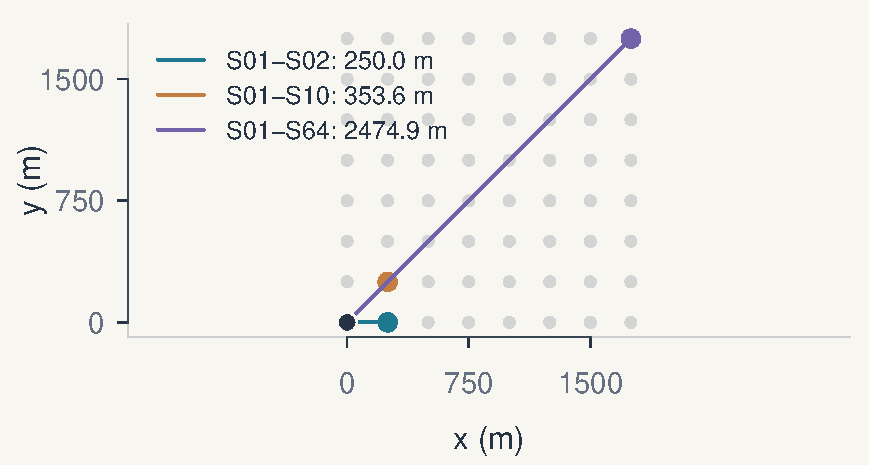
\includegraphics[width=9.85cm,height=4.6cm,keepaspectratio]{Risultati/Figure/05_distanze_piano.pdf}
\vspace{1.5mm}
\PSmall{Distanze in metri. Il passo ortogonale è 250 m; la diagonale della cella è $250\sqrt 2$ m.}

\end{minipage}\end{lrbox}
\typeout{FULLBOX:019:PilotLeftBox:\the\ht\PilotLeftBox:\the\dp\PilotLeftBox}

\begin{lrbox}{\PilotRightBox}
\begin{minipage}[t]{7.55cm}\raggedright\color{Ink}\fontsize{11.3}{14.8}\selectfont
\PBody{La metrica usa la stessa unità sui due assi. La matrice delle distanze deve essere simmetrica, non negativa e nulla sulla diagonale.}
\vspace{2.5mm}
\PInfo{La diagonale principale collega ogni sito a se stesso. La escluderemo quando cercheremo vicini o coppie distinte.}
\PCode{R · matrice delle distanze}{019_esempio.R}
\end{minipage}\end{lrbox}
\typeout{FULLBOX:019:PilotRightBox:\the\ht\PilotRightBox:\the\dp\PilotRightBox}

\begin{tikzpicture}[remember picture,overlay]
\PilotChrome{La distanza euclidea nel piano locale}{II · COORDINATE E DISTANZE}{19}{Il calcolo della distanza richiede assi e unità coerenti.}
\node[anchor=north west,inner sep=0] at([xshift=.96cm,yshift=-2.13cm]current page.north west){\usebox{\PilotLeftBox}};
\node[anchor=north west,inner sep=0] at([xshift=11.52cm,yshift=-2.13cm]current page.north west){\usebox{\PilotRightBox}};
\node[anchor=north east,inner sep=0] at([xshift=17.65cm,yshift=-12.06cm]current page.north west){\color{Classical}\fontsize{7.7}{9.2}\selectfont\href{../../03_Notebook_svolti/M11_Locus/M11_N03.html}{M11\_N03 · notebook svolto}};
\end{tikzpicture}\end{frame}

\begin{frame}[plain]\hypertarget{slide20}{}
\bookmark[level=1,page=20]{Traslazioni e rotazioni conservano le distanze}
\begin{lrbox}{\TitleBox}
\begin{minipage}[t]{17.7cm}\raggedright\color{Ink}\fontsize{11.3}{14.8}\selectfont
\color{Navy}\bfseries\fontsize{20.6}{24.5}\selectfont Traslazioni e rotazioni conservano le distanze
\end{minipage}\end{lrbox}
\typeout{FULLBOX:020:TitleBox:\the\ht\TitleBox:\the\dp\TitleBox}

\begin{lrbox}{\RecallBox}
\begin{minipage}[t]{14.3cm}\raggedright\color{Ink}\fontsize{11.3}{14.8}\selectfont
\fontsize{10.3}{13.8}\selectfont Gli invarianti geometrici sono controlli concreti della funzione di distanza.
\end{minipage}\end{lrbox}
\typeout{FULLBOX:020:RecallBox:\the\ht\RecallBox:\the\dp\RecallBox}

\begin{lrbox}{\PilotLeftBox}
\begin{minipage}[t]{10.05cm}\raggedright\color{Ink}\fontsize{11.3}{14.8}\selectfont
\[s_i^\star=Q\,s_i+b,\qquad Q^\top Q=I\]
\[\|s_i^\star-s_j^\star\|=\|s_i-s_j\|\]
\PInfo{Cambiare origine o ruotare rigidamente gli assi non cambia le distanze. Moltiplicare tutte le coordinate per un fattore $a$ moltiplica le distanze per $|a|$.}

\end{minipage}\end{lrbox}
\typeout{FULLBOX:020:PilotLeftBox:\the\ht\PilotLeftBox:\the\dp\PilotLeftBox}

\begin{lrbox}{\PilotRightBox}
\begin{minipage}[t]{7.55cm}\raggedright\color{Ink}\fontsize{11.3}{14.8}\selectfont
\PBody{Queste proprietà offrono controlli del programma. Una conversione da metri a chilometri deve ridurre tutte le distanze di un fattore mille.}
\vspace{2.5mm}
\PBody{Una proiezione geografica non è in generale una rotazione rigida: la sua distorsione va valutata nell’area d’uso.}
\vspace{2.5mm}
\PCode{R · verificare traslazione e scala}{020_esempio.R}
\end{minipage}\end{lrbox}
\typeout{FULLBOX:020:PilotRightBox:\the\ht\PilotRightBox:\the\dp\PilotRightBox}

\begin{tikzpicture}[remember picture,overlay]
\PilotChrome{Traslazioni e rotazioni conservano le distanze}{II · COORDINATE E DISTANZE}{20}{Gli invarianti geometrici sono controlli concreti della funzione di distanza.}
\node[anchor=north west,inner sep=0] at([xshift=.96cm,yshift=-2.13cm]current page.north west){\usebox{\PilotLeftBox}};
\node[anchor=north west,inner sep=0] at([xshift=11.52cm,yshift=-2.13cm]current page.north west){\usebox{\PilotRightBox}};
\node[anchor=north east,inner sep=0] at([xshift=17.65cm,yshift=-12.06cm]current page.north west){\color{Classical}\fontsize{7.7}{9.2}\selectfont\href{../../03_Notebook_svolti/M11_Locus/M11_N03.html}{M11\_N03 · notebook svolto}};
\end{tikzpicture}\end{frame}

\begin{frame}[plain]\hypertarget{slide21}{}
\bookmark[level=1,page=21]{Distanza orizzontale, tridimensionale o di percorso}
\begin{lrbox}{\TitleBox}
\begin{minipage}[t]{17.7cm}\raggedright\color{Ink}\fontsize{11.3}{14.8}\selectfont
\color{Navy}\bfseries\fontsize{20.6}{24.5}\selectfont Distanza orizzontale, tridimensionale o di percorso
\end{minipage}\end{lrbox}
\typeout{FULLBOX:021:TitleBox:\the\ht\TitleBox:\the\dp\TitleBox}

\begin{lrbox}{\RecallBox}
\begin{minipage}[t]{14.3cm}\raggedright\color{Ink}\fontsize{11.3}{14.8}\selectfont
\fontsize{10.3}{13.8}\selectfont La distanza deve rappresentare la relazione fisica o il compito che si vuole studiare.
\end{minipage}\end{lrbox}
\typeout{FULLBOX:021:RecallBox:\the\ht\RecallBox:\the\dp\RecallBox}

\begin{lrbox}{\PilotLeftBox}
\begin{minipage}[t]{10.05cm}\raggedright\color{Ink}\fontsize{11.3}{14.8}\selectfont
{\fontsize{10.2}{13.1}\selectfont\renewcommand{\arraystretch}{1.45}\begin{tabular}{@{}p{4.1cm}p{4.9cm}@{}}\toprule
\textbf{Metrica} & \textbf{Che cosa rappresenta}\\\midrule
$\sqrt{\Delta x^2+\Delta y^2}$ & Separazione orizzontale nel piano\\
$\sqrt{\Delta x^2+\Delta y^2+\Delta h^2}$ & Segmento tridimensionale\\
Lunghezza su una rete & Percorso vincolato a collegamenti\\
Distanza di costo & Percorso pesato da resistenze dichiarate\\
\bottomrule\end{tabular}}

\end{minipage}\end{lrbox}
\typeout{FULLBOX:021:PilotLeftBox:\the\ht\PilotLeftBox:\the\dp\PilotLeftBox}

\begin{lrbox}{\PilotRightBox}
\begin{minipage}[t]{7.55cm}\raggedright\color{Ink}\fontsize{11.3}{14.8}\selectfont
\PBody{La quota può entrare nella distanza, ma cambia il significato di vicino. Una distanza lungo il reticolo idrografico richiede una rete e una regola di percorso.}
\vspace{2.5mm}
\PInfo{In questo modulo i pesi principali usano la distanza orizzontale locale. La scelta resta costante quando confrontiamo Moran, copertura e interpolazione.}
\PBody{Non aggiungiamo una variabile al calcolo della distanza soltanto perché è numerica.}
\vspace{2.5mm}

\end{minipage}\end{lrbox}
\typeout{FULLBOX:021:PilotRightBox:\the\ht\PilotRightBox:\the\dp\PilotRightBox}

\begin{tikzpicture}[remember picture,overlay]
\PilotChrome{Distanza orizzontale, tridimensionale o di percorso}{II · COORDINATE E DISTANZE}{21}{La distanza deve rappresentare la relazione fisica o il compito che si vuole studiare.}
\node[anchor=north west,inner sep=0] at([xshift=.96cm,yshift=-2.13cm]current page.north west){\usebox{\PilotLeftBox}};
\node[anchor=north west,inner sep=0] at([xshift=11.52cm,yshift=-2.13cm]current page.north west){\usebox{\PilotRightBox}};
\end{tikzpicture}\end{frame}

\begin{frame}[plain]\hypertarget{slide22}{}
\bookmark[level=1,page=22]{Sulla sfera si misura un arco}
\begin{lrbox}{\TitleBox}
\begin{minipage}[t]{17.7cm}\raggedright\color{Ink}\fontsize{11.3}{14.8}\selectfont
\color{Navy}\bfseries\fontsize{20.6}{24.5}\selectfont Sulla sfera si misura un arco
\end{minipage}\end{lrbox}
\typeout{FULLBOX:022:TitleBox:\the\ht\TitleBox:\the\dp\TitleBox}

\begin{lrbox}{\RecallBox}
\begin{minipage}[t]{14.3cm}\raggedright\color{Ink}\fontsize{11.3}{14.8}\selectfont
\fontsize{10.3}{13.8}\selectfont La scelta della geometria terrestre appartiene alla definizione della distanza.
\end{minipage}\end{lrbox}
\typeout{FULLBOX:022:RecallBox:\the\ht\RecallBox:\the\dp\RecallBox}

\begin{lrbox}{\PilotLeftBox}
\begin{minipage}[t]{10.05cm}\raggedright\color{Ink}\fontsize{11.3}{14.8}\selectfont
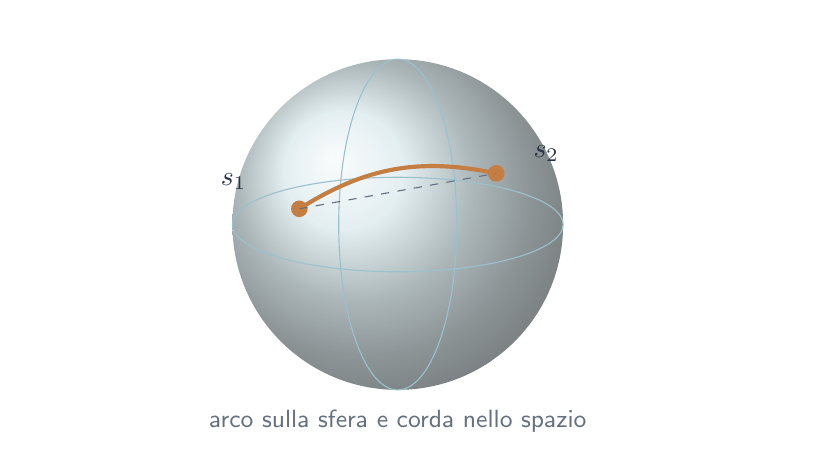
\begin{tikzpicture}[x=1cm,y=1cm]
\path[use as bounding box](-.1,-.15) rectangle(9.7,5.1);
\shade[ball color=GeoA!22,opacity=.75](4.6,2.6)circle(2.1);
\draw[GeoA!45](4.6,2.6)ellipse(2.1 and .6);
\draw[GeoA!45](4.6,2.6)ellipse(.75 and 2.1);
\fill[GeoB](3.35,2.8)circle(3pt);
\fill[GeoB](5.85,3.25)circle(3pt);
\draw[GeoB,line width=1.5pt](3.35,2.8)to[bend left=22](5.85,3.25);
\draw[Muted,dashed](3.35,2.8)--(5.85,3.25);
\node[pLabel,anchor=east]at(2.8,3.15){$s_1$};
\node[pLabel,anchor=west]at(6.2,3.5){$s_2$};
\node[pNote]at(4.6,.1){arco sulla sfera e corda nello spazio};
\end{tikzpicture}

\end{minipage}\end{lrbox}
\typeout{FULLBOX:022:PilotLeftBox:\the\ht\PilotLeftBox:\the\dp\PilotLeftBox}

\begin{lrbox}{\PilotRightBox}
\begin{minipage}[t]{7.55cm}\raggedright\color{Ink}\fontsize{11.3}{14.8}\selectfont
\PBody{Longitudine e latitudine sono angoli. Sulla sfera, la separazione più breve lungo la superficie è un arco di cerchio massimo.}
\vspace{2.5mm}
\PInfo{La Terra non è una sfera perfetta. Il modello sferico è un’approssimazione esplicita; un calcolo ellissoidale richiede i parametri del riferimento adottato.}
\PBody{La funzione del laboratorio usa un raggio sferico dichiarato pari a 6\,371\,000 m. L’uscita è quindi in metri.}
\vspace{2.5mm}

\end{minipage}\end{lrbox}
\typeout{FULLBOX:022:PilotRightBox:\the\ht\PilotRightBox:\the\dp\PilotRightBox}

\begin{tikzpicture}[remember picture,overlay]
\PilotChrome{Sulla sfera si misura un arco}{II · COORDINATE E DISTANZE}{22}{La scelta della geometria terrestre appartiene alla definizione della distanza.}
\node[anchor=north west,inner sep=0] at([xshift=.96cm,yshift=-2.13cm]current page.north west){\usebox{\PilotLeftBox}};
\node[anchor=north west,inner sep=0] at([xshift=11.52cm,yshift=-2.13cm]current page.north west){\usebox{\PilotRightBox}};
\node[anchor=north east,inner sep=0] at([xshift=17.65cm,yshift=-12.06cm]current page.north west){\color{Classical}\fontsize{7.7}{9.2}\selectfont\href{../../03_Notebook_svolti/M11_Locus/M11_N04.html}{M11\_N04 · notebook svolto}};
\end{tikzpicture}\end{frame}

\begin{frame}[plain]\hypertarget{slide23}{}
\bookmark[level=1,page=23]{Haversine: angoli in radianti e unità esplicite}
\begin{lrbox}{\TitleBox}
\begin{minipage}[t]{17.7cm}\raggedright\color{Ink}\fontsize{11.3}{14.8}\selectfont
\color{Navy}\bfseries\fontsize{20.6}{24.5}\selectfont Haversine: angoli in radianti e unità esplicite
\end{minipage}\end{lrbox}
\typeout{FULLBOX:023:TitleBox:\the\ht\TitleBox:\the\dp\TitleBox}

\begin{lrbox}{\RecallBox}
\begin{minipage}[t]{14.3cm}\raggedright\color{Ink}\fontsize{11.3}{14.8}\selectfont
\fontsize{10.3}{13.8}\selectfont Una formula corretta produce distanze sbagliate se riceve gradi al posto di radianti.
\end{minipage}\end{lrbox}
\typeout{FULLBOX:023:RecallBox:\the\ht\RecallBox:\the\dp\RecallBox}

\begin{lrbox}{\PilotLeftBox}
\begin{minipage}[t]{10.05cm}\raggedright\color{Ink}\fontsize{11.3}{14.8}\selectfont
\[a=\sin^2\frac{\Delta\varphi}{2}+\cos\varphi_1\cos\varphi_2\sin^2\frac{\Delta\lambda}{2}\]
\[d=2R\operatorname{atan2}\!\left(\sqrt a,\sqrt{1-a}\right)\]
\PInfo{$\varphi$ indica la latitudine e $\lambda$ la longitudine, entrambe in radianti. Per stabilità numerica si limita $a$ all’intervallo $[0,1]$.}

\end{minipage}\end{lrbox}
\typeout{FULLBOX:023:PilotLeftBox:\the\ht\PilotLeftBox:\the\dp\PilotLeftBox}

\begin{lrbox}{\PilotRightBox}
\begin{minipage}[t]{7.55cm}\raggedright\color{Ink}\fontsize{11.3}{14.8}\selectfont
\PBody{La distanza deve essere zero tra punti coincidenti, simmetrica e finita. Il notebook controlla anche un arco semplice di ampiezza nota.}
\vspace{2.5mm}
\PBody{La funzione esplicita permette di vedere la conversione dei gradi. L’ordine degli argomenti resta longitudine, latitudine.}
\vspace{2.5mm}
\PCode{R · arco sulla sfera}{023_esempio.R}
\end{minipage}\end{lrbox}
\typeout{FULLBOX:023:PilotRightBox:\the\ht\PilotRightBox:\the\dp\PilotRightBox}

\begin{tikzpicture}[remember picture,overlay]
\PilotChrome{Haversine: angoli in radianti e unità esplicite}{II · COORDINATE E DISTANZE}{23}{Una formula corretta produce distanze sbagliate se riceve gradi al posto di radianti.}
\node[anchor=north west,inner sep=0] at([xshift=.96cm,yshift=-2.13cm]current page.north west){\usebox{\PilotLeftBox}};
\node[anchor=north west,inner sep=0] at([xshift=11.52cm,yshift=-2.13cm]current page.north west){\usebox{\PilotRightBox}};
\node[anchor=north east,inner sep=0] at([xshift=17.65cm,yshift=-12.06cm]current page.north west){\color{Classical}\fontsize{7.7}{9.2}\selectfont\href{../../03_Notebook_svolti/M11_Locus/M11_N04.html}{M11\_N04 · notebook svolto}};
\end{tikzpicture}\end{frame}

\begin{frame}[plain]\hypertarget{slide24}{}
\bookmark[level=1,page=24]{Un grado non rappresenta una lunghezza fissa}
\begin{lrbox}{\TitleBox}
\begin{minipage}[t]{17.7cm}\raggedright\color{Ink}\fontsize{11.3}{14.8}\selectfont
\color{Navy}\bfseries\fontsize{20.6}{24.5}\selectfont Un grado non rappresenta una lunghezza fissa
\end{minipage}\end{lrbox}
\typeout{FULLBOX:024:TitleBox:\the\ht\TitleBox:\the\dp\TitleBox}

\begin{lrbox}{\RecallBox}
\begin{minipage}[t]{14.3cm}\raggedright\color{Ink}\fontsize{11.3}{14.8}\selectfont
\fontsize{10.3}{13.8}\selectfont Le differenze angolari devono essere trasformate con una geometria dichiarata.
\end{minipage}\end{lrbox}
\typeout{FULLBOX:024:RecallBox:\the\ht\RecallBox:\the\dp\RecallBox}

\begin{lrbox}{\PilotLeftBox}
\begin{minipage}[t]{10.05cm}\raggedright\color{Ink}\fontsize{11.3}{14.8}\selectfont
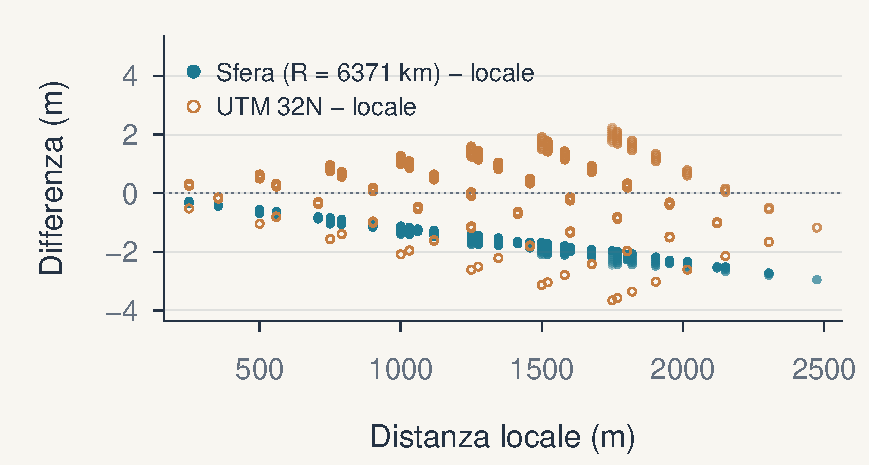
\includegraphics[width=9.85cm,height=5.25cm,keepaspectratio]{Risultati/Figure/06_distanze_geografiche.pdf}
\vspace{1.5mm}
\PSmall{Scarti delle distanze sferiche e UTM rispetto alle distanze locali, sulle stesse coppie di siti.}

\end{minipage}\end{lrbox}
\typeout{FULLBOX:024:PilotLeftBox:\the\ht\PilotLeftBox:\the\dp\PilotLeftBox}

\begin{lrbox}{\PilotRightBox}
\begin{minipage}[t]{7.55cm}\raggedright\color{Ink}\fontsize{11.3}{14.8}\selectfont
\PBody{La lunghezza di un grado di longitudine dipende dalla latitudine. Applicare una sola conversione ai due assi trascura questa geometria.}
\vspace{2.5mm}
\PInfo{In una piccola area una proiezione adatta offre coordinate metriche comode. L’adeguatezza resta legata all’area e alla precisione richiesta.}
\PBody{Il confronto tra distanze locali, sferiche e proiettate serve a capire le assunzioni, non a imporre un’identità tra rappresentazioni costruite diversamente.}
\vspace{2.5mm}

\end{minipage}\end{lrbox}
\typeout{FULLBOX:024:PilotRightBox:\the\ht\PilotRightBox:\the\dp\PilotRightBox}

\begin{tikzpicture}[remember picture,overlay]
\PilotChrome{Un grado non rappresenta una lunghezza fissa}{II · COORDINATE E DISTANZE}{24}{Le differenze angolari devono essere trasformate con una geometria dichiarata.}
\node[anchor=north west,inner sep=0] at([xshift=.96cm,yshift=-2.13cm]current page.north west){\usebox{\PilotLeftBox}};
\node[anchor=north west,inner sep=0] at([xshift=11.52cm,yshift=-2.13cm]current page.north west){\usebox{\PilotRightBox}};
\node[anchor=north east,inner sep=0] at([xshift=17.65cm,yshift=-12.06cm]current page.north west){\color{Classical}\fontsize{7.7}{9.2}\selectfont\href{../../03_Notebook_svolti/M11_Locus/M11_N04.html}{M11\_N04 · notebook svolto}};
\end{tikzpicture}\end{frame}

\begin{frame}[plain]\hypertarget{slide25}{}
\bookmark[level=1,page=25]{Il CRS è un insieme di regole, non un’etichetta}
\begin{lrbox}{\TitleBox}
\begin{minipage}[t]{17.7cm}\raggedright\color{Ink}\fontsize{11.3}{14.8}\selectfont
\color{Navy}\bfseries\fontsize{20.6}{24.5}\selectfont Il CRS è un insieme di regole, non un’etichetta
\end{minipage}\end{lrbox}
\typeout{FULLBOX:025:TitleBox:\the\ht\TitleBox:\the\dp\TitleBox}

\begin{lrbox}{\RecallBox}
\begin{minipage}[t]{14.3cm}\raggedright\color{Ink}\fontsize{11.3}{14.8}\selectfont
\fontsize{10.3}{13.8}\selectfont Un CRS corretto deve essere noto dalla provenienza dei dati o da una verifica indipendente.
\end{minipage}\end{lrbox}
\typeout{FULLBOX:025:RecallBox:\the\ht\RecallBox:\the\dp\RecallBox}

\begin{lrbox}{\PilotLeftBox}
\begin{minipage}[t]{10.05cm}\raggedright\color{Ink}\fontsize{11.3}{14.8}\selectfont
{\fontsize{10.2}{13.1}\selectfont\renewcommand{\arraystretch}{1.45}\begin{tabular}{@{}p{3.3cm}p{5.7cm}@{}}\toprule
\textbf{Elemento} & \textbf{Funzione}\\\midrule
Riferimento geodetico & Colloca il sistema rispetto alla Terra\\
Assi e unità & Definiscono ordine e significato dei numeri\\
Proiezione, se presente & Trasforma la superficie in un piano\\
Area d’uso & Indica dove il sistema è appropriato\\
\bottomrule\end{tabular}}

\end{minipage}\end{lrbox}
\typeout{FULLBOX:025:PilotLeftBox:\the\ht\PilotLeftBox:\the\dp\PilotLeftBox}

\begin{lrbox}{\PilotRightBox}
\begin{minipage}[t]{7.55cm}\raggedright\color{Ink}\fontsize{11.3}{14.8}\selectfont
\PBody{Il sistema di riferimento delle coordinate descrive come interpretare le geometrie. Il codice di un catalogo ne identifica una definizione.}
\vspace{2.5mm}
\PInfo{Per rendere esplicito l’ordine longitudine--latitudine usiamo \texttt{OGC:CRS84}. Il bersaglio proiettato del laboratorio è WGS 84 / UTM zona 32N, EPSG:32632.}
\PBody{La scelta è riferita all’esempio sintetico vicino a 9° E e 45° N. Non costituisce una regola universale per ogni dataset.}
\vspace{2.5mm}

\end{minipage}\end{lrbox}
\typeout{FULLBOX:025:PilotRightBox:\the\ht\PilotRightBox:\the\dp\PilotRightBox}

\begin{tikzpicture}[remember picture,overlay]
\PilotChrome{Il CRS è un insieme di regole, non un’etichetta}{II · COORDINATE E DISTANZE}{25}{Un CRS corretto deve essere noto dalla provenienza dei dati o da una verifica indipendente.}
\node[anchor=north west,inner sep=0] at([xshift=.96cm,yshift=-2.13cm]current page.north west){\usebox{\PilotLeftBox}};
\node[anchor=north west,inner sep=0] at([xshift=11.52cm,yshift=-2.13cm]current page.north west){\usebox{\PilotRightBox}};
\node[anchor=north east,inner sep=0] at([xshift=17.65cm,yshift=-12.06cm]current page.north west){\color{Classical}\fontsize{7.7}{9.2}\selectfont\href{../../03_Notebook_svolti/M11_Locus/M11_N05.html}{M11\_N05 · notebook svolto}};
\end{tikzpicture}\end{frame}

\begin{frame}[plain]\hypertarget{slide26}{}
\bookmark[level=1,page=26]{Costruire una geometria conservando la tabella}
\begin{lrbox}{\TitleBox}
\begin{minipage}[t]{17.7cm}\raggedright\color{Ink}\fontsize{11.3}{14.8}\selectfont
\color{Navy}\bfseries\fontsize{20.6}{24.5}\selectfont Costruire una geometria conservando la tabella
\end{minipage}\end{lrbox}
\typeout{FULLBOX:026:TitleBox:\the\ht\TitleBox:\the\dp\TitleBox}

\begin{lrbox}{\RecallBox}
\begin{minipage}[t]{14.3cm}\raggedright\color{Ink}\fontsize{11.3}{14.8}\selectfont
\fontsize{10.3}{13.8}\selectfont Costruire una geometria richiede dati interpretabili prima della chiamata al software.
\end{minipage}\end{lrbox}
\typeout{FULLBOX:026:RecallBox:\the\ht\RecallBox:\the\dp\RecallBox}

\begin{lrbox}{\PilotLeftBox}
\begin{minipage}[t]{10.05cm}\raggedright\color{Ink}\fontsize{11.3}{14.8}\selectfont
\[(\mathrm{id},z,\lambda,\varphi)\quad\longrightarrow\quad \text{oggetto sf}\]
{\fontsize{10.2}{13.1}\selectfont\renewcommand{\arraystretch}{1.45}\begin{tabular}{@{}p{3.5cm}p{5.5cm}@{}}\toprule
\textbf{Controllo} & \textbf{Risultato atteso}\\\midrule
Numero di geometrie & 64 punti\\
Attributi & ID e misure preservati\\
Ordine degli assi & Longitudine, latitudine\\
CRS dichiarato & OGC:CRS84\\
\bottomrule\end{tabular}}

\end{minipage}\end{lrbox}
\typeout{FULLBOX:026:PilotLeftBox:\the\ht\PilotLeftBox:\the\dp\PilotLeftBox}

\begin{lrbox}{\PilotRightBox}
\begin{minipage}[t]{7.55cm}\raggedright\color{Ink}\fontsize{11.3}{14.8}\selectfont
\PBody{La geometria viene creata dalle colonne geografiche. Con \texttt{remove=FALSE} conserviamo anche i valori originari nella tabella.}
\vspace{2.5mm}
\PInfo{La creazione dell’oggetto assegna il significato dichiarato ai numeri. Non corregge un ordine degli assi sbagliato.}
\PCode{R · punti geografici}{026_esempio.R}
\end{minipage}\end{lrbox}
\typeout{FULLBOX:026:PilotRightBox:\the\ht\PilotRightBox:\the\dp\PilotRightBox}

\begin{tikzpicture}[remember picture,overlay]
\PilotChrome{Costruire una geometria conservando la tabella}{II · COORDINATE E DISTANZE}{26}{Costruire una geometria richiede dati interpretabili prima della chiamata al software.}
\node[anchor=north west,inner sep=0] at([xshift=.96cm,yshift=-2.13cm]current page.north west){\usebox{\PilotLeftBox}};
\node[anchor=north west,inner sep=0] at([xshift=11.52cm,yshift=-2.13cm]current page.north west){\usebox{\PilotRightBox}};
\node[anchor=north east,inner sep=0] at([xshift=17.65cm,yshift=-12.06cm]current page.north west){\color{Classical}\fontsize{7.7}{9.2}\selectfont\href{../../03_Notebook_svolti/M11_Locus/M11_N05.html}{M11\_N05 · notebook svolto}};
\end{tikzpicture}\end{frame}

\begin{frame}[plain]\hypertarget{slide27}{}
\bookmark[level=1,page=27]{Trasformare cambia i numeri, conserva il luogo}
\begin{lrbox}{\TitleBox}
\begin{minipage}[t]{17.7cm}\raggedright\color{Ink}\fontsize{11.3}{14.8}\selectfont
\color{Navy}\bfseries\fontsize{20.6}{24.5}\selectfont Trasformare cambia i numeri, conserva il luogo
\end{minipage}\end{lrbox}
\typeout{FULLBOX:027:TitleBox:\the\ht\TitleBox:\the\dp\TitleBox}

\begin{lrbox}{\RecallBox}
\begin{minipage}[t]{14.3cm}\raggedright\color{Ink}\fontsize{11.3}{14.8}\selectfont
\fontsize{10.3}{13.8}\selectfont La trasformazione usa due definizioni di riferimento; non basta cambiare il nome del CRS.
\end{minipage}\end{lrbox}
\typeout{FULLBOX:027:RecallBox:\the\ht\RecallBox:\the\dp\RecallBox}

\begin{lrbox}{\PilotLeftBox}
\begin{minipage}[t]{10.05cm}\raggedright\color{Ink}\fontsize{11.3}{14.8}\selectfont
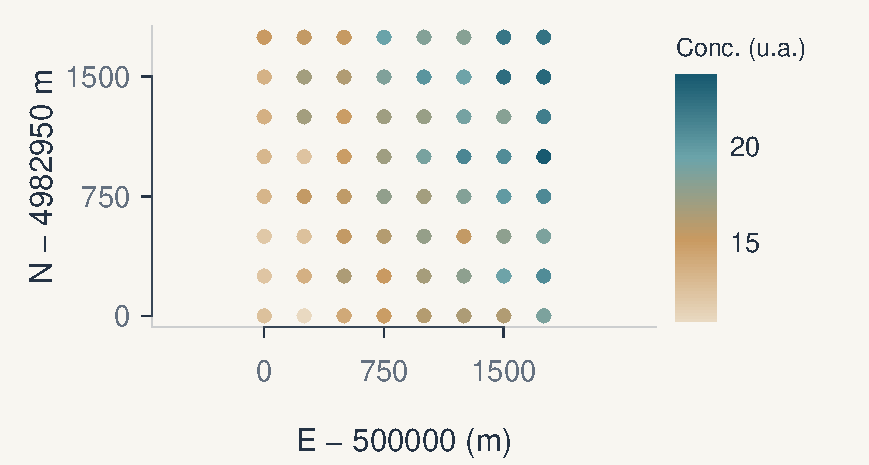
\includegraphics[width=9.85cm,height=5.25cm,keepaspectratio]{Risultati/Figure/07_proiezione_UTM.pdf}
\vspace{1.5mm}
\PSmall{Geometria sintetica in UTM 32N. Gli assi sottraggono origini dichiarate per rendere leggibili le coordinate.}

\end{minipage}\end{lrbox}
\typeout{FULLBOX:027:PilotLeftBox:\the\ht\PilotLeftBox:\the\dp\PilotLeftBox}

\begin{lrbox}{\PilotRightBox}
\begin{minipage}[t]{7.55cm}\raggedright\color{Ink}\fontsize{11.3}{14.8}\selectfont
\PBody{\texttt{st\_transform} calcola nuove coordinate usando il CRS di origine e quello di destinazione. Le unità del bersaglio diventano metri.}
\vspace{2.5mm}
\PInfo{Il calcolo è verificato con \texttt{sf} e le librerie geografiche effettivamente caricate. Le versioni sono registrate con i risultati.}
\PCode{R · proiettare i punti}{027_esempio.R}
\end{minipage}\end{lrbox}
\typeout{FULLBOX:027:PilotRightBox:\the\ht\PilotRightBox:\the\dp\PilotRightBox}

\begin{tikzpicture}[remember picture,overlay]
\PilotChrome{Trasformare cambia i numeri, conserva il luogo}{II · COORDINATE E DISTANZE}{27}{La trasformazione usa due definizioni di riferimento; non basta cambiare il nome del CRS.}
\node[anchor=north west,inner sep=0] at([xshift=.96cm,yshift=-2.13cm]current page.north west){\usebox{\PilotLeftBox}};
\node[anchor=north west,inner sep=0] at([xshift=11.52cm,yshift=-2.13cm]current page.north west){\usebox{\PilotRightBox}};
\node[anchor=north east,inner sep=0] at([xshift=17.65cm,yshift=-12.06cm]current page.north west){\color{Classical}\fontsize{7.7}{9.2}\selectfont\href{../../03_Notebook_svolti/M11_Locus/M11_N05.html}{M11\_N05 · notebook svolto}};
\end{tikzpicture}\end{frame}

\begin{frame}[plain]\hypertarget{slide28}{}
\bookmark[level=1,page=28]{Il controllo di ritorno verifica la trasformazione}
\begin{lrbox}{\TitleBox}
\begin{minipage}[t]{17.7cm}\raggedright\color{Ink}\fontsize{11.3}{14.8}\selectfont
\color{Navy}\bfseries\fontsize{20.6}{24.5}\selectfont Il controllo di ritorno verifica la trasformazione
\end{minipage}\end{lrbox}
\typeout{FULLBOX:028:TitleBox:\the\ht\TitleBox:\the\dp\TitleBox}

\begin{lrbox}{\RecallBox}
\begin{minipage}[t]{14.3cm}\raggedright\color{Ink}\fontsize{11.3}{14.8}\selectfont
\fontsize{10.3}{13.8}\selectfont Il controllo di ritorno verifica il procedimento numerico, mentre la provenienza verifica il riferimento.
\end{minipage}\end{lrbox}
\typeout{FULLBOX:028:RecallBox:\the\ht\RecallBox:\the\dp\RecallBox}

\begin{lrbox}{\PilotLeftBox}
\begin{minipage}[t]{10.05cm}\raggedright\color{Ink}\fontsize{11.3}{14.8}\selectfont
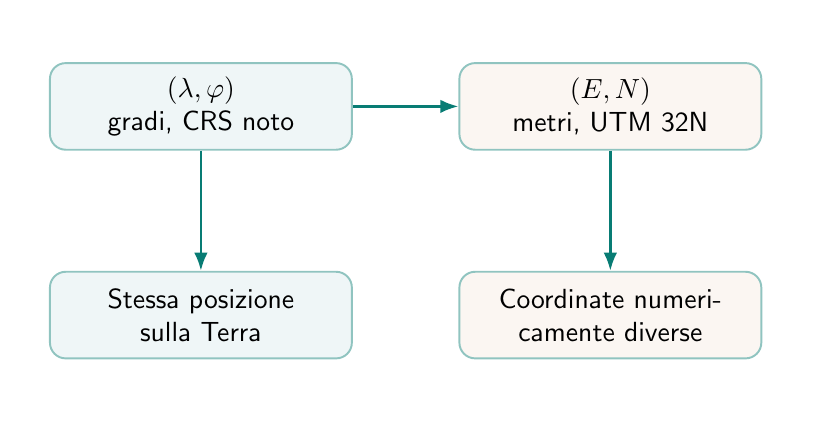
\begin{tikzpicture}[x=1cm,y=1cm]
\path[use as bounding box](-.1,-.15) rectangle(9.7,4.8);
\node[pFlow,text width=3.6cm,fill=GeoA!7] (a) at(2.1,3.8){$(\lambda,\varphi)$\\gradi, CRS noto};
\node[pFlow,text width=3.6cm,fill=GeoB!7] (b) at(7.3,3.8){$(E,N)$\\metri, UTM 32N};
\node[pFlow,text width=3.6cm,fill=GeoA!7] (c) at(2.1,1.15){Stessa posizione sulla Terra};
\node[pFlow,text width=3.6cm,fill=GeoB!7] (d) at(7.3,1.15){Coordinate numericamente diverse};
\draw[pEdge] (a) -- (b);
\draw[pEdge] (a) -- (c);
\draw[pEdge] (b) -- (d);
\end{tikzpicture}

\end{minipage}\end{lrbox}
\typeout{FULLBOX:028:PilotLeftBox:\the\ht\PilotLeftBox:\the\dp\PilotLeftBox}

\begin{lrbox}{\PilotRightBox}
\begin{minipage}[t]{7.55cm}\raggedright\color{Ink}\fontsize{11.3}{14.8}\selectfont
\PBody{Trasformiamo i punti in UTM e torniamo a OGC:CRS84. La tolleranza del confronto è in gradi.}
\vspace{2.5mm}
\PInfo{Un ritorno accurato mostra coerenza numerica delle trasformazioni. La correttezza del CRS iniziale richiede una verifica della provenienza.}
\PCode{R · ritorno alle coordinate iniziali}{028_esempio.R}
\end{minipage}\end{lrbox}
\typeout{FULLBOX:028:PilotRightBox:\the\ht\PilotRightBox:\the\dp\PilotRightBox}

\begin{tikzpicture}[remember picture,overlay]
\PilotChrome{Il controllo di ritorno verifica la trasformazione}{II · COORDINATE E DISTANZE}{28}{Il controllo di ritorno verifica il procedimento numerico, mentre la provenienza verifica il riferimento.}
\node[anchor=north west,inner sep=0] at([xshift=.96cm,yshift=-2.13cm]current page.north west){\usebox{\PilotLeftBox}};
\node[anchor=north west,inner sep=0] at([xshift=11.52cm,yshift=-2.13cm]current page.north west){\usebox{\PilotRightBox}};
\node[anchor=north east,inner sep=0] at([xshift=17.65cm,yshift=-12.06cm]current page.north west){\color{Classical}\fontsize{7.7}{9.2}\selectfont\href{../../03_Notebook_svolti/M11_Locus/M11_N05.html}{M11\_N05 · notebook svolto}};
\end{tikzpicture}\end{frame}

\begin{frame}[plain]\hypertarget{slide29}{}
\bookmark[level=1,page=29]{Rietichettare lascia invariati i numeri}
\begin{lrbox}{\TitleBox}
\begin{minipage}[t]{17.7cm}\raggedright\color{Ink}\fontsize{11.3}{14.8}\selectfont
\color{Navy}\bfseries\fontsize{20.6}{24.5}\selectfont Rietichettare lascia invariati i numeri
\end{minipage}\end{lrbox}
\typeout{FULLBOX:029:TitleBox:\the\ht\TitleBox:\the\dp\TitleBox}

\begin{lrbox}{\RecallBox}
\begin{minipage}[t]{14.3cm}\raggedright\color{Ink}\fontsize{11.3}{14.8}\selectfont
\fontsize{10.3}{13.8}\selectfont Cambiare la definizione del CRS e trasformare le coordinate sono operazioni distinte.
\end{minipage}\end{lrbox}
\typeout{FULLBOX:029:RecallBox:\the\ht\RecallBox:\the\dp\RecallBox}

\begin{lrbox}{\PilotLeftBox}
\begin{minipage}[t]{10.05cm}\raggedright\color{Ink}\fontsize{11.3}{14.8}\selectfont
{\fontsize{10.2}{13.1}\selectfont\renewcommand{\arraystretch}{1.45}\begin{tabular}{@{}p{4.0cm}p{5.0cm}@{}}\toprule
\textbf{Operazione} & \textbf{Effetto}\\\midrule
\texttt{st\_set\_crs} & Assegna o sostituisce la definizione del CRS\\
\texttt{st\_transform} & Calcola coordinate nel CRS di destinazione\\
Assegnazione errata & Numeri invariati, significato geografico alterato\\
Correzione documentata & Richiede conoscere il vero CRS dei numeri\\
\bottomrule\end{tabular}}

\end{minipage}\end{lrbox}
\typeout{FULLBOX:029:PilotLeftBox:\the\ht\PilotLeftBox:\the\dp\PilotLeftBox}

\begin{lrbox}{\PilotRightBox}
\begin{minipage}[t]{7.55cm}\raggedright\color{Ink}\fontsize{11.3}{14.8}\selectfont
\PBody{Assegnare EPSG:32632 a una coppia di gradi non la converte in metri. La geometria diventa numericamente identica e semanticamente errata.}
\vspace{2.5mm}
\PInfo{Nel notebook N06 l’operazione sbagliata è costruita in un oggetto separato e il relativo avviso è acquisito come parte dell’esperimento.}
\PCode{R · osservare prima di rietichettare}{029_esempio.R}
\end{minipage}\end{lrbox}
\typeout{FULLBOX:029:PilotRightBox:\the\ht\PilotRightBox:\the\dp\PilotRightBox}

\begin{tikzpicture}[remember picture,overlay]
\PilotChrome{Rietichettare lascia invariati i numeri}{II · COORDINATE E DISTANZE}{29}{Cambiare la definizione del CRS e trasformare le coordinate sono operazioni distinte.}
\node[anchor=north west,inner sep=0] at([xshift=.96cm,yshift=-2.13cm]current page.north west){\usebox{\PilotLeftBox}};
\node[anchor=north west,inner sep=0] at([xshift=11.52cm,yshift=-2.13cm]current page.north west){\usebox{\PilotRightBox}};
\node[anchor=north east,inner sep=0] at([xshift=17.65cm,yshift=-12.06cm]current page.north west){\color{Classical}\fontsize{7.7}{9.2}\selectfont\href{../../03_Notebook_svolti/M11_Locus/M11_N06.html}{M11\_N06 · notebook svolto}};
\end{tikzpicture}\end{frame}

\begin{frame}[plain]\hypertarget{slide30}{}
\bookmark[level=1,page=30]{Confrontare distanze senza confondere i sistemi}
\begin{lrbox}{\TitleBox}
\begin{minipage}[t]{17.7cm}\raggedright\color{Ink}\fontsize{11.3}{14.8}\selectfont
\color{Navy}\bfseries\fontsize{20.6}{24.5}\selectfont Confrontare distanze senza confondere i sistemi
\end{minipage}\end{lrbox}
\typeout{FULLBOX:030:TitleBox:\the\ht\TitleBox:\the\dp\TitleBox}

\begin{lrbox}{\RecallBox}
\begin{minipage}[t]{14.3cm}\raggedright\color{Ink}\fontsize{11.3}{14.8}\selectfont
\fontsize{10.3}{13.8}\selectfont Le unità uguali rendono possibile un confronto, ma non garantiscono l’equivalenza dei calcoli.
\end{minipage}\end{lrbox}
\typeout{FULLBOX:030:RecallBox:\the\ht\RecallBox:\the\dp\RecallBox}

\begin{lrbox}{\PilotLeftBox}
\begin{minipage}[t]{10.05cm}\raggedright\color{Ink}\fontsize{11.3}{14.8}\selectfont
{\fontsize{10.2}{13.1}\selectfont\renewcommand{\arraystretch}{1.45}\begin{tabular}{@{}p{3.8cm}p{5.2cm}@{}}\toprule
\textbf{Calcolo} & \textbf{Interpretazione}\\\midrule
Euclidea locale & Metri nel sistema convenzionale della griglia\\
Haversine & Arco nel modello terrestre sferico\\
Euclidea in UTM & Distanza nel piano della proiezione\\
Geodetica ellissoidale & Richiede riferimento e algoritmo espliciti\\
\bottomrule\end{tabular}}

\end{minipage}\end{lrbox}
\typeout{FULLBOX:030:PilotLeftBox:\the\ht\PilotLeftBox:\the\dp\PilotLeftBox}

\begin{lrbox}{\PilotRightBox}
\begin{minipage}[t]{7.55cm}\raggedright\color{Ink}\fontsize{11.3}{14.8}\selectfont
\PBody{Le distanze vanno confrontate sulla stessa coppia di ID, mantenendo visibile il metodo usato.}
\vspace{2.5mm}
\PInfo{Una differenza piccola non autorizza a confondere i sistemi. Una differenza inattesa richiede di verificare unità, ordine degli assi, riferimento e area d’uso.}
\PCode{R · la stessa coppia di siti}{030_esempio.R}
\end{minipage}\end{lrbox}
\typeout{FULLBOX:030:PilotRightBox:\the\ht\PilotRightBox:\the\dp\PilotRightBox}

\begin{tikzpicture}[remember picture,overlay]
\PilotChrome{Confrontare distanze senza confondere i sistemi}{II · COORDINATE E DISTANZE}{30}{Le unità uguali rendono possibile un confronto, ma non garantiscono l’equivalenza dei calcoli.}
\node[anchor=north west,inner sep=0] at([xshift=.96cm,yshift=-2.13cm]current page.north west){\usebox{\PilotLeftBox}};
\node[anchor=north west,inner sep=0] at([xshift=11.52cm,yshift=-2.13cm]current page.north west){\usebox{\PilotRightBox}};
\node[anchor=north east,inner sep=0] at([xshift=17.65cm,yshift=-12.06cm]current page.north west){\color{Classical}\fontsize{7.7}{9.2}\selectfont\href{../../03_Notebook_svolti/M11_Locus/M11_N05.html}{M11\_N05 · notebook svolto}};
\end{tikzpicture}\end{frame}

\begin{frame}[plain]\hypertarget{slide31}{}
\bookmark[level=1,page=31]{Laboratorio: coordinate sotto controllo}
\begin{lrbox}{\TitleBox}
\begin{minipage}[t]{17.7cm}\raggedright\color{Ink}\fontsize{11.3}{14.8}\selectfont
\color{Navy}\bfseries\fontsize{20.6}{24.5}\selectfont Laboratorio: coordinate sotto controllo
\end{minipage}\end{lrbox}
\typeout{FULLBOX:031:TitleBox:\the\ht\TitleBox:\the\dp\TitleBox}

\begin{lrbox}{\RecallBox}
\begin{minipage}[t]{14.3cm}\raggedright\color{Ink}\fontsize{11.3}{14.8}\selectfont
\fontsize{10.3}{13.8}\selectfont Le operazioni spaziali diventano interpretabili quando i riferimenti sono espliciti e verificati.
\end{minipage}\end{lrbox}
\typeout{FULLBOX:031:RecallBox:\the\ht\RecallBox:\the\dp\RecallBox}

\begin{lrbox}{\PilotLeftBox}
\begin{minipage}[t]{10.05cm}\raggedright\color{Ink}\fontsize{11.3}{14.8}\selectfont
\PLab{https://marzione00.github.io/Lab_Geo/\#laboratorio/m11-coordinate}{Esperimento online · coordinate e metrica}
{\fontsize{10.2}{13.1}\selectfont\renewcommand{\arraystretch}{1.45}\begin{tabular}{@{}p{4.1cm}p{4.9cm}@{}}\toprule
\textbf{Attività} & \textbf{Prova da conservare}\\\midrule
N02: assi invertiti & Limiti globali e posizione attesa\\
N03: distanza euclidea & Simmetria, diagonale, invarianti\\
N04: haversine & Radianti, raggio, casi semplici\\
N05: trasformazione & CRS di origine e controllo di ritorno\\
N06: rietichettatura & Numeri invariati, significato alterato\\
\bottomrule\end{tabular}}

\end{minipage}\end{lrbox}
\typeout{FULLBOX:031:PilotLeftBox:\the\ht\PilotLeftBox:\the\dp\PilotLeftBox}

\begin{lrbox}{\PilotRightBox}
\begin{minipage}[t]{7.55cm}\raggedright\color{Ink}\fontsize{11.3}{14.8}\selectfont
\PBody{La consegna include una piccola tabella delle distanze fra coppie note. Ogni colonna deve indicare unità e metodo.}
\vspace{2.5mm}
\PInfo{La precisione numerica della trasformazione e l’accuratezza geografica dei dati sono due proprietà diverse. Il controllo deve nominarle correttamente.}
\PBody{Con riferimenti e distanze definiti possiamo passare a confini, appartenenze e vicinati.}
\vspace{2.5mm}

\end{minipage}\end{lrbox}
\typeout{FULLBOX:031:PilotRightBox:\the\ht\PilotRightBox:\the\dp\PilotRightBox}

\begin{tikzpicture}[remember picture,overlay]
\PilotChrome{Laboratorio: coordinate sotto controllo}{II · COORDINATE E DISTANZE}{31}{Le operazioni spaziali diventano interpretabili quando i riferimenti sono espliciti e verificati.}
\node[anchor=north west,inner sep=0] at([xshift=.96cm,yshift=-2.13cm]current page.north west){\usebox{\PilotLeftBox}};
\node[anchor=north west,inner sep=0] at([xshift=11.52cm,yshift=-2.13cm]current page.north west){\usebox{\PilotRightBox}};
\node[anchor=north east,inner sep=0] at([xshift=17.65cm,yshift=-12.06cm]current page.north west){\color{Classical}\fontsize{7.7}{9.2}\selectfont\href{../../03_Notebook_svolti/M11_Locus/M11_N06.html}{M11\_N06 · notebook svolto}};
\end{tikzpicture}\end{frame}

\begin{frame}[plain]\hypertarget{slide32}{}
\bookmark[level=0,page=32]{III · CARTE E APPARTENENZE}
\bookmark[level=1,page=32]{Una carta rende visibile una scelta statistica}
\begin{lrbox}{\TitleBox}
\begin{minipage}[t]{17.7cm}\raggedright\color{Ink}\fontsize{11.3}{14.8}\selectfont
\color{Navy}\bfseries\fontsize{20.6}{24.5}\selectfont Una carta rende visibile una scelta statistica
\end{minipage}\end{lrbox}
\typeout{FULLBOX:032:TitleBox:\the\ht\TitleBox:\the\dp\TitleBox}

\begin{lrbox}{\RecallBox}
\begin{minipage}[t]{14.3cm}\raggedright\color{Ink}\fontsize{11.3}{14.8}\selectfont
\fontsize{10.3}{13.8}\selectfont La legenda deve spiegare il dato, l’unità e l’eventuale modello dietro la rappresentazione.
\end{minipage}\end{lrbox}
\typeout{FULLBOX:032:RecallBox:\the\ht\RecallBox:\the\dp\RecallBox}

\begin{lrbox}{\PilotLeftBox}
\begin{minipage}[t]{10.05cm}\raggedright\color{Ink}\fontsize{11.3}{14.8}\selectfont
{\fontsize{10.2}{13.1}\selectfont\renewcommand{\arraystretch}{1.45}\begin{tabular}{@{}p{3.2cm}p{5.8cm}@{}}\toprule
\textbf{Elemento della carta} & \textbf{Scelta che comunica}\\\midrule
Punti & Luoghi delle osservazioni\\
Poligoni & Unità territoriali e supporti\\
Colore & Valori e scala di confronto\\
Linee & Confini, percorsi o vicinati\\
Superficie continua & Una stima tra i campioni\\
\bottomrule\end{tabular}}

\end{minipage}\end{lrbox}
\typeout{FULLBOX:032:PilotLeftBox:\the\ht\PilotLeftBox:\the\dp\PilotLeftBox}

\begin{lrbox}{\PilotRightBox}
\begin{minipage}[t]{7.55cm}\raggedright\color{Ink}\fontsize{11.3}{14.8}\selectfont
\PBody{La forma grafica influenza la lettura del risultato. Ogni elemento deve corrispondere a un oggetto definito nell’analisi.}
\vspace{2.5mm}
\PInfo{Un’interpolazione richiede di mostrare anche i siti utilizzati. Senza campioni visibili, la carta nasconde dove la previsione è sostenuta dai dati.}
\PBody{Manteniamo gli stessi limiti cromatici quando due pannelli devono essere confrontati.}
\vspace{2.5mm}

\end{minipage}\end{lrbox}
\typeout{FULLBOX:032:PilotRightBox:\the\ht\PilotRightBox:\the\dp\PilotRightBox}

\begin{tikzpicture}[remember picture,overlay]
\PilotChrome{Una carta rende visibile una scelta statistica}{III · CARTE E APPARTENENZE}{32}{La legenda deve spiegare il dato, l’unità e l’eventuale modello dietro la rappresentazione.}
\node[anchor=north west,inner sep=0] at([xshift=.96cm,yshift=-2.13cm]current page.north west){\usebox{\PilotLeftBox}};
\node[anchor=north west,inner sep=0] at([xshift=11.52cm,yshift=-2.13cm]current page.north west){\usebox{\PilotRightBox}};
\node[anchor=north east,inner sep=0] at([xshift=17.65cm,yshift=-12.06cm]current page.north west){\color{Classical}\fontsize{7.7}{9.2}\selectfont\href{../../03_Notebook_svolti/M11_Locus/M11_N07.html}{M11\_N07 · notebook svolto}};
\end{tikzpicture}\end{frame}

\begin{frame}[plain]\hypertarget{slide33}{}
\bookmark[level=1,page=33]{Scale cromatiche comparabili, assi proporzionati}
\begin{lrbox}{\TitleBox}
\begin{minipage}[t]{17.7cm}\raggedright\color{Ink}\fontsize{11.3}{14.8}\selectfont
\color{Navy}\bfseries\fontsize{20.6}{24.5}\selectfont Scale cromatiche comparabili, assi proporzionati
\end{minipage}\end{lrbox}
\typeout{FULLBOX:033:TitleBox:\the\ht\TitleBox:\the\dp\TitleBox}

\begin{lrbox}{\RecallBox}
\begin{minipage}[t]{14.3cm}\raggedright\color{Ink}\fontsize{11.3}{14.8}\selectfont
\fontsize{10.3}{13.8}\selectfont Il confronto visivo richiede scale e unità costanti.
\end{minipage}\end{lrbox}
\typeout{FULLBOX:033:RecallBox:\the\ht\RecallBox:\the\dp\RecallBox}

\begin{lrbox}{\PilotLeftBox}
\begin{minipage}[t]{10.05cm}\raggedright\color{Ink}\fontsize{11.3}{14.8}\selectfont
{\fontsize{10.2}{13.1}\selectfont\renewcommand{\arraystretch}{1.45}\begin{tabular}{@{}p{4.0cm}p{5.0cm}@{}}\toprule
\textbf{Controllo} & \textbf{Perché serve}\\\midrule
Rapporto 1:1 degli assi & Un metro ha la stessa lunghezza grafica\\
Unità nei titoli degli assi & Evita di confondere gradi e metri\\
Scala cromatica comune & Permette confronti quantitativi\\
Legenda esplicita & Distingue valore, gruppo e previsione\\
Simboli dei campioni & Mostra il supporto osservativo\\
\bottomrule\end{tabular}}

\end{minipage}\end{lrbox}
\typeout{FULLBOX:033:PilotLeftBox:\the\ht\PilotLeftBox:\the\dp\PilotLeftBox}

\begin{lrbox}{\PilotRightBox}
\begin{minipage}[t]{7.55cm}\raggedright\color{Ink}\fontsize{11.3}{14.8}\selectfont
\PBody{Un rettangolo disegnato come un quadrato altera la percezione delle distanze. Il parametro \texttt{asp=1} conserva le proporzioni nel piano locale.}
\vspace{2.5mm}
\PInfo{La palette rappresenta la concentrazione in u.a. Non indica da sola una soglia ambientale o una classe di rischio.}
\PCode{R · geometria della carta}{033_esempio.R}
\end{minipage}\end{lrbox}
\typeout{FULLBOX:033:PilotRightBox:\the\ht\PilotRightBox:\the\dp\PilotRightBox}

\begin{tikzpicture}[remember picture,overlay]
\PilotChrome{Scale cromatiche comparabili, assi proporzionati}{III · CARTE E APPARTENENZE}{33}{Il confronto visivo richiede scale e unità costanti.}
\node[anchor=north west,inner sep=0] at([xshift=.96cm,yshift=-2.13cm]current page.north west){\usebox{\PilotLeftBox}};
\node[anchor=north west,inner sep=0] at([xshift=11.52cm,yshift=-2.13cm]current page.north west){\usebox{\PilotRightBox}};
\node[anchor=north east,inner sep=0] at([xshift=17.65cm,yshift=-12.06cm]current page.north west){\color{Classical}\fontsize{7.7}{9.2}\selectfont\href{../../03_Notebook_svolti/M11_Locus/M11_N07.html}{M11\_N07 · notebook svolto}};
\end{tikzpicture}\end{frame}

\begin{frame}[plain]\hypertarget{slide34}{}
\bookmark[level=1,page=34]{Aggregare assegna campioni a unità territoriali}
\begin{lrbox}{\TitleBox}
\begin{minipage}[t]{17.7cm}\raggedright\color{Ink}\fontsize{11.3}{14.8}\selectfont
\color{Navy}\bfseries\fontsize{20.6}{24.5}\selectfont Aggregare assegna campioni a unità territoriali
\end{minipage}\end{lrbox}
\typeout{FULLBOX:034:TitleBox:\the\ht\TitleBox:\the\dp\TitleBox}

\begin{lrbox}{\RecallBox}
\begin{minipage}[t]{14.3cm}\raggedright\color{Ink}\fontsize{11.3}{14.8}\selectfont
\fontsize{10.3}{13.8}\selectfont Una media territoriale deve indicare quali campioni contiene e con quali pesi.
\end{minipage}\end{lrbox}
\typeout{FULLBOX:034:RecallBox:\the\ht\RecallBox:\the\dp\RecallBox}

\begin{lrbox}{\PilotLeftBox}
\begin{minipage}[t]{10.05cm}\raggedright\color{Ink}\fontsize{11.3}{14.8}\selectfont
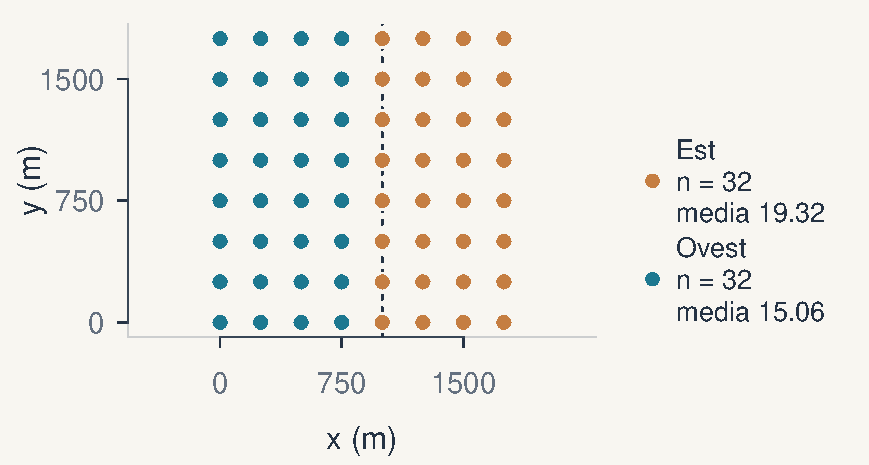
\includegraphics[width=9.85cm,height=5.25cm,keepaspectratio]{Risultati/Figure/08_confini_aggregazioni.pdf}
\vspace{1.5mm}
\PSmall{La partizione del dataset separa Ovest ($x<1000$) ed Est ($x\ge1000$): 32 siti per gruppo.}

\end{minipage}\end{lrbox}
\typeout{FULLBOX:034:PilotLeftBox:\the\ht\PilotLeftBox:\the\dp\PilotLeftBox}

\begin{lrbox}{\PilotRightBox}
\begin{minipage}[t]{7.55cm}\raggedright\color{Ink}\fontsize{11.3}{14.8}\selectfont
\PBody{Per ogni area calcoliamo numerosità e media dei campioni assegnati. I conteggi sono necessari per interpretare le medie.}
\vspace{2.5mm}
\PInfo{Questa soglia descrittiva a 1000 m è diversa dalla separazione a 1250 m usata nel test previsionale. Le due operazioni hanno scopi diversi.}
\PCode{R · aggregazione documentata}{034_esempio.R}
\end{minipage}\end{lrbox}
\typeout{FULLBOX:034:PilotRightBox:\the\ht\PilotRightBox:\the\dp\PilotRightBox}

\begin{tikzpicture}[remember picture,overlay]
\PilotChrome{Aggregare assegna campioni a unità territoriali}{III · CARTE E APPARTENENZE}{34}{Una media territoriale deve indicare quali campioni contiene e con quali pesi.}
\node[anchor=north west,inner sep=0] at([xshift=.96cm,yshift=-2.13cm]current page.north west){\usebox{\PilotLeftBox}};
\node[anchor=north west,inner sep=0] at([xshift=11.52cm,yshift=-2.13cm]current page.north west){\usebox{\PilotRightBox}};
\node[anchor=north east,inner sep=0] at([xshift=17.65cm,yshift=-12.06cm]current page.north west){\color{Classical}\fontsize{7.7}{9.2}\selectfont\href{../../03_Notebook_svolti/M11_Locus/M11_N08.html}{M11\_N08 · notebook svolto}};
\end{tikzpicture}\end{frame}

\begin{frame}[plain]\hypertarget{slide35}{}
\bookmark[level=1,page=35]{Confini diversi producono riassunti diversi}
\begin{lrbox}{\TitleBox}
\begin{minipage}[t]{17.7cm}\raggedright\color{Ink}\fontsize{11.3}{14.8}\selectfont
\color{Navy}\bfseries\fontsize{20.6}{24.5}\selectfont Confini diversi producono riassunti diversi
\end{minipage}\end{lrbox}
\typeout{FULLBOX:035:TitleBox:\the\ht\TitleBox:\the\dp\TitleBox}

\begin{lrbox}{\RecallBox}
\begin{minipage}[t]{14.3cm}\raggedright\color{Ink}\fontsize{11.3}{14.8}\selectfont
\fontsize{10.3}{13.8}\selectfont I confini sono parte dell’analisi e devono essere motivati insieme alle statistiche.
\end{minipage}\end{lrbox}
\typeout{FULLBOX:035:RecallBox:\the\ht\RecallBox:\the\dp\RecallBox}

\begin{lrbox}{\PilotLeftBox}
\begin{minipage}[t]{10.05cm}\raggedright\color{Ink}\fontsize{11.3}{14.8}\selectfont
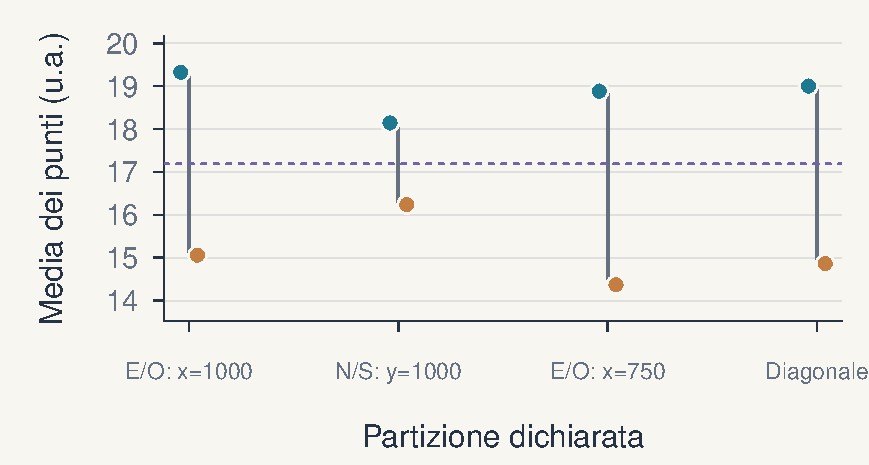
\includegraphics[width=9.85cm,height=5.25cm,keepaspectratio]{Risultati/Figure/09_aggregazioni_alternative.pdf}
\vspace{1.5mm}
\PSmall{Gli stessi siti possono essere raggruppati con partizioni diverse. Cambiano le unità della sintesi.}

\end{minipage}\end{lrbox}
\typeout{FULLBOX:035:PilotLeftBox:\the\ht\PilotLeftBox:\the\dp\PilotLeftBox}

\begin{lrbox}{\PilotRightBox}
\begin{minipage}[t]{7.55cm}\raggedright\color{Ink}\fontsize{11.3}{14.8}\selectfont
\PBody{Cambiare la scala o la disposizione dei confini può cambiare le medie, la variabilità tra aree e le relazioni osservate.}
\vspace{2.5mm}
\PInfo{Questa sensibilità è legata al problema delle unità areali modificabili. Un risultato riferito a una partizione non diventa automaticamente una proprietà delle singole persone, rocce o misure.}
\PBody{Il confronto tra partizioni è una verifica di sensibilità; la partizione principale deve essere motivata prima di scegliere la figura più convincente.}
\vspace{2.5mm}

\end{minipage}\end{lrbox}
\typeout{FULLBOX:035:PilotRightBox:\the\ht\PilotRightBox:\the\dp\PilotRightBox}

\begin{tikzpicture}[remember picture,overlay]
\PilotChrome{Confini diversi producono riassunti diversi}{III · CARTE E APPARTENENZE}{35}{I confini sono parte dell’analisi e devono essere motivati insieme alle statistiche.}
\node[anchor=north west,inner sep=0] at([xshift=.96cm,yshift=-2.13cm]current page.north west){\usebox{\PilotLeftBox}};
\node[anchor=north west,inner sep=0] at([xshift=11.52cm,yshift=-2.13cm]current page.north west){\usebox{\PilotRightBox}};
\end{tikzpicture}\end{frame}

\begin{frame}[plain]\hypertarget{slide36}{}
\bookmark[level=1,page=36]{Una regola semiaperta evita doppie assegnazioni}
\begin{lrbox}{\TitleBox}
\begin{minipage}[t]{17.7cm}\raggedright\color{Ink}\fontsize{11.3}{14.8}\selectfont
\color{Navy}\bfseries\fontsize{20.6}{24.5}\selectfont Una regola semiaperta evita doppie assegnazioni
\end{minipage}\end{lrbox}
\typeout{FULLBOX:036:TitleBox:\the\ht\TitleBox:\the\dp\TitleBox}

\begin{lrbox}{\RecallBox}
\begin{minipage}[t]{14.3cm}\raggedright\color{Ink}\fontsize{11.3}{14.8}\selectfont
\fontsize{10.3}{13.8}\selectfont Una partizione richiede copertura completa e assenza di sovrapposizioni.
\end{minipage}\end{lrbox}
\typeout{FULLBOX:036:RecallBox:\the\ht\RecallBox:\the\dp\RecallBox}

\begin{lrbox}{\PilotLeftBox}
\begin{minipage}[t]{10.05cm}\raggedright\color{Ink}\fontsize{11.3}{14.8}\selectfont
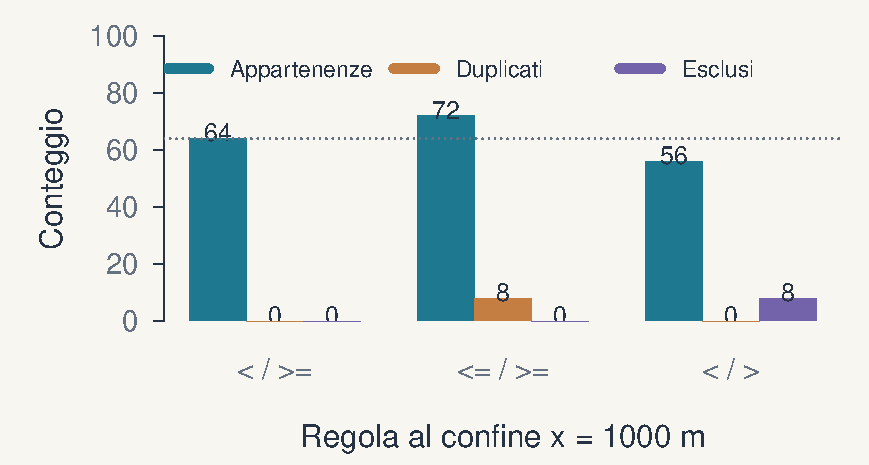
\includegraphics[width=9.85cm,height=5.25cm,keepaspectratio]{Risultati/Figure/10_confini_semiaperti.pdf}
\vspace{1.5mm}
\PSmall{Il confine $x=1000$ appartiene a Est. La partizione copre tutti i siti senza intersezioni.}

\end{minipage}\end{lrbox}
\typeout{FULLBOX:036:PilotLeftBox:\the\ht\PilotLeftBox:\the\dp\PilotLeftBox}

\begin{lrbox}{\PilotRightBox}
\begin{minipage}[t]{7.55cm}\raggedright\color{Ink}\fontsize{11.3}{14.8}\selectfont
\PBody{Le condizioni $x<1000$ e $x\ge1000$ definiscono due insiemi disgiunti e completi. Un punto sul confine riceve un’unica appartenenza.}
\vspace{2.5mm}
\PInfo{Con veri poligoni, il predicato spaziale e la gestione dei bordi devono essere dichiarati. “Dentro” e “interseca” non sono sinonimi.}
\PCode{R · verificare la partizione}{036_esempio.R}
\end{minipage}\end{lrbox}
\typeout{FULLBOX:036:PilotRightBox:\the\ht\PilotRightBox:\the\dp\PilotRightBox}

\begin{tikzpicture}[remember picture,overlay]
\PilotChrome{Una regola semiaperta evita doppie assegnazioni}{III · CARTE E APPARTENENZE}{36}{Una partizione richiede copertura completa e assenza di sovrapposizioni.}
\node[anchor=north west,inner sep=0] at([xshift=.96cm,yshift=-2.13cm]current page.north west){\usebox{\PilotLeftBox}};
\node[anchor=north west,inner sep=0] at([xshift=11.52cm,yshift=-2.13cm]current page.north west){\usebox{\PilotRightBox}};
\node[anchor=north east,inner sep=0] at([xshift=17.65cm,yshift=-12.06cm]current page.north west){\color{Classical}\fontsize{7.7}{9.2}\selectfont\href{../../03_Notebook_svolti/M11_Locus/M11_N08.html}{M11\_N08 · notebook svolto}};
\end{tikzpicture}\end{frame}

\begin{frame}[plain]\hypertarget{slide37}{}
\bookmark[level=1,page=37]{Un sito può appartenere a più regioni}
\begin{lrbox}{\TitleBox}
\begin{minipage}[t]{17.7cm}\raggedright\color{Ink}\fontsize{11.3}{14.8}\selectfont
\color{Navy}\bfseries\fontsize{20.6}{24.5}\selectfont Un sito può appartenere a più regioni
\end{minipage}\end{lrbox}
\typeout{FULLBOX:037:TitleBox:\the\ht\TitleBox:\the\dp\TitleBox}

\begin{lrbox}{\RecallBox}
\begin{minipage}[t]{14.3cm}\raggedright\color{Ink}\fontsize{11.3}{14.8}\selectfont
\fontsize{10.3}{13.8}\selectfont Quando le aree si sovrappongono, il numero delle relazioni può superare il numero dei siti.
\end{minipage}\end{lrbox}
\typeout{FULLBOX:037:RecallBox:\the\ht\RecallBox:\the\dp\RecallBox}

\begin{lrbox}{\PilotLeftBox}
\begin{minipage}[t]{10.05cm}\raggedright\color{Ink}\fontsize{11.3}{14.8}\selectfont
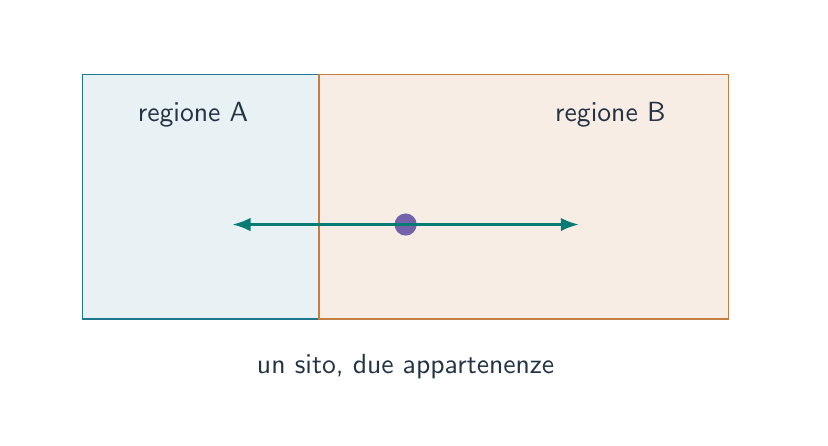
\begin{tikzpicture}[x=1cm,y=1cm]
\path[use as bounding box](-.1,-.15) rectangle(9.7,4.8);
\filldraw[fill=GeoA!10,draw=GeoA](.6,1.1)rectangle(5.8,4.2);
\filldraw[fill=GeoB!14,draw=GeoB](3.6,1.1)rectangle(8.8,4.2);
\node[pLabel]at(2,3.7){regione A};
\node[pLabel]at(7.3,3.7){regione B};
\fill[GeoC](4.7,2.3)circle(4pt);
\node[pLabel]at(4.7,.5){un sito, due appartenenze};
\draw[pEdge](4.7,2.3)--(2.5,2.3);
\draw[pEdge](4.7,2.3)--(6.9,2.3);
\end{tikzpicture}

\end{minipage}\end{lrbox}
\typeout{FULLBOX:037:PilotLeftBox:\the\ht\PilotLeftBox:\the\dp\PilotLeftBox}

\begin{lrbox}{\PilotRightBox}
\begin{minipage}[t]{7.55cm}\raggedright\color{Ink}\fontsize{11.3}{14.8}\selectfont
\PBody{Consideriamo A definita da $x\le1250$ e B da $x\ge750$. L’intervallo comune comprende tre colonne della griglia.}
\vspace{2.5mm}
\PInfo{Le appartenenze sono 88, i siti restano 64 e quelli con due appartenenze sono 24. Il join descrive relazioni, non crea nuovi campioni.}
\PBody{Una regione amministrativa disgiunta e un insieme di aree di influenza sovrapposte richiedono convenzioni differenti.}
\vspace{2.5mm}

\end{minipage}\end{lrbox}
\typeout{FULLBOX:037:PilotRightBox:\the\ht\PilotRightBox:\the\dp\PilotRightBox}

\begin{tikzpicture}[remember picture,overlay]
\PilotChrome{Un sito può appartenere a più regioni}{III · CARTE E APPARTENENZE}{37}{Quando le aree si sovrappongono, il numero delle relazioni può superare il numero dei siti.}
\node[anchor=north west,inner sep=0] at([xshift=.96cm,yshift=-2.13cm]current page.north west){\usebox{\PilotLeftBox}};
\node[anchor=north west,inner sep=0] at([xshift=11.52cm,yshift=-2.13cm]current page.north west){\usebox{\PilotRightBox}};
\node[anchor=north east,inner sep=0] at([xshift=17.65cm,yshift=-12.06cm]current page.north west){\color{Classical}\fontsize{7.7}{9.2}\selectfont\href{../../03_Notebook_svolti/M11_Locus/M11_N09.html}{M11\_N09 · notebook svolto}};
\end{tikzpicture}\end{frame}

\begin{frame}[plain]\hypertarget{slide38}{}
\bookmark[level=1,page=38]{Controllare la cardinalità dopo un join}
\begin{lrbox}{\TitleBox}
\begin{minipage}[t]{17.7cm}\raggedright\color{Ink}\fontsize{11.3}{14.8}\selectfont
\color{Navy}\bfseries\fontsize{20.6}{24.5}\selectfont Controllare la cardinalità dopo un join
\end{minipage}\end{lrbox}
\typeout{FULLBOX:038:TitleBox:\the\ht\TitleBox:\the\dp\TitleBox}

\begin{lrbox}{\RecallBox}
\begin{minipage}[t]{14.3cm}\raggedright\color{Ink}\fontsize{11.3}{14.8}\selectfont
\fontsize{10.3}{13.8}\selectfont Il controllo delle molteplicità impedisce di confondere relazioni e osservazioni.
\end{minipage}\end{lrbox}
\typeout{FULLBOX:038:RecallBox:\the\ht\RecallBox:\the\dp\RecallBox}

\begin{lrbox}{\PilotLeftBox}
\begin{minipage}[t]{10.05cm}\raggedright\color{Ink}\fontsize{11.3}{14.8}\selectfont
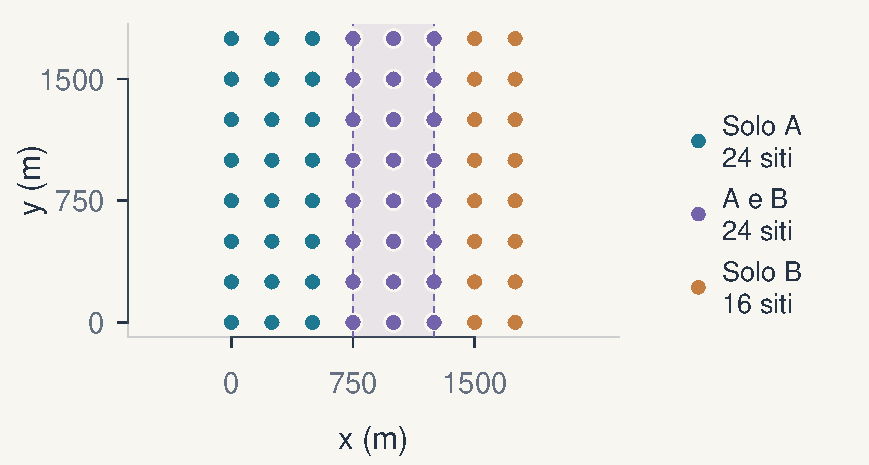
\includegraphics[width=9.85cm,height=5.25cm,keepaspectratio]{Risultati/Figure/11_join_sovrapposto.pdf}
\vspace{1.5mm}
\PSmall{Due regioni sovrapposte generano più righe per gli stessi identificativi.}

\end{minipage}\end{lrbox}
\typeout{FULLBOX:038:PilotLeftBox:\the\ht\PilotLeftBox:\the\dp\PilotLeftBox}

\begin{lrbox}{\PilotRightBox}
\begin{minipage}[t]{7.55cm}\raggedright\color{Ink}\fontsize{11.3}{14.8}\selectfont
\PBody{Dopo un join confrontiamo righe, ID distinti e molteplicità. Ogni variazione deve avere una spiegazione geometrica o tabellare.}
\vspace{2.5mm}
\PInfo{Fare la media di tutte le righe del join assegnerebbe peso doppio ai siti nell’intersezione. È una scelta statistica, anche se avviene involontariamente.}
\PCode{R · contare le appartenenze}{038_esempio.R}
\end{minipage}\end{lrbox}
\typeout{FULLBOX:038:PilotRightBox:\the\ht\PilotRightBox:\the\dp\PilotRightBox}

\begin{tikzpicture}[remember picture,overlay]
\PilotChrome{Controllare la cardinalità dopo un join}{III · CARTE E APPARTENENZE}{38}{Il controllo delle molteplicità impedisce di confondere relazioni e osservazioni.}
\node[anchor=north west,inner sep=0] at([xshift=.96cm,yshift=-2.13cm]current page.north west){\usebox{\PilotLeftBox}};
\node[anchor=north west,inner sep=0] at([xshift=11.52cm,yshift=-2.13cm]current page.north west){\usebox{\PilotRightBox}};
\node[anchor=north east,inner sep=0] at([xshift=17.65cm,yshift=-12.06cm]current page.north west){\color{Classical}\fontsize{7.7}{9.2}\selectfont\href{../../03_Notebook_svolti/M11_Locus/M11_N09.html}{M11\_N09 · notebook svolto}};
\end{tikzpicture}\end{frame}

\begin{frame}[plain]\hypertarget{slide39}{}
\bookmark[level=1,page=39]{Il buffer definisce una domanda locale}
\begin{lrbox}{\TitleBox}
\begin{minipage}[t]{17.7cm}\raggedright\color{Ink}\fontsize{11.3}{14.8}\selectfont
\color{Navy}\bfseries\fontsize{20.6}{24.5}\selectfont Il buffer definisce una domanda locale
\end{minipage}\end{lrbox}
\typeout{FULLBOX:039:TitleBox:\the\ht\TitleBox:\the\dp\TitleBox}

\begin{lrbox}{\RecallBox}
\begin{minipage}[t]{14.3cm}\raggedright\color{Ink}\fontsize{11.3}{14.8}\selectfont
\fontsize{10.3}{13.8}\selectfont Centro, raggio, metrica e regola del bordo definiscono il contenuto del buffer.
\end{minipage}\end{lrbox}
\typeout{FULLBOX:039:RecallBox:\the\ht\RecallBox:\the\dp\RecallBox}

\begin{lrbox}{\PilotLeftBox}
\begin{minipage}[t]{10.05cm}\raggedright\color{Ink}\fontsize{11.3}{14.8}\selectfont
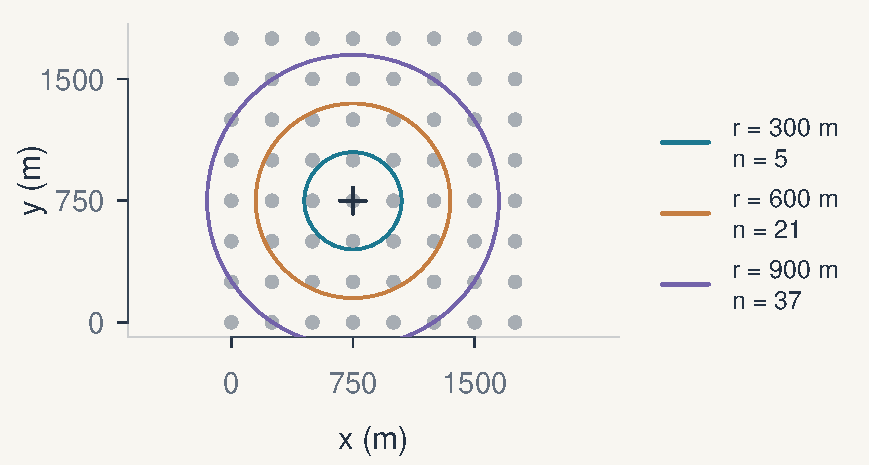
\includegraphics[width=9.85cm,height=5.25cm,keepaspectratio]{Risultati/Figure/12_buffer_raggi.pdf}
\vspace{1.5mm}
\PSmall{Centro $(750,750)$ m; raggi 300, 600 e 900 m. I campioni inclusi cambiano con la scala.}

\end{minipage}\end{lrbox}
\typeout{FULLBOX:039:PilotLeftBox:\the\ht\PilotLeftBox:\the\dp\PilotLeftBox}

\begin{lrbox}{\PilotRightBox}
\begin{minipage}[t]{7.55cm}\raggedright\color{Ink}\fontsize{11.3}{14.8}\selectfont
\PBody{Un buffer include i siti entro una distanza dal centro. La regola del laboratorio comprende anche i punti esattamente sul raggio.}
\vspace{2.5mm}
\PInfo{La media nel buffer riassume i campioni selezionati. Non è automaticamente la media areale del disco.}
\PCode{R · inclusione nel buffer}{039_esempio.R}
\end{minipage}\end{lrbox}
\typeout{FULLBOX:039:PilotRightBox:\the\ht\PilotRightBox:\the\dp\PilotRightBox}

\begin{tikzpicture}[remember picture,overlay]
\PilotChrome{Il buffer definisce una domanda locale}{III · CARTE E APPARTENENZE}{39}{Centro, raggio, metrica e regola del bordo definiscono il contenuto del buffer.}
\node[anchor=north west,inner sep=0] at([xshift=.96cm,yshift=-2.13cm]current page.north west){\usebox{\PilotLeftBox}};
\node[anchor=north west,inner sep=0] at([xshift=11.52cm,yshift=-2.13cm]current page.north west){\usebox{\PilotRightBox}};
\node[anchor=north east,inner sep=0] at([xshift=17.65cm,yshift=-12.06cm]current page.north west){\color{Classical}\fontsize{7.7}{9.2}\selectfont\href{../../03_Notebook_svolti/M11_Locus/M11_N10.html}{M11\_N10 · notebook svolto}};
\end{tikzpicture}\end{frame}

\begin{frame}[plain]\hypertarget{slide40}{}
\bookmark[level=1,page=40]{La media locale cambia quando cambia il raggio}
\begin{lrbox}{\TitleBox}
\begin{minipage}[t]{17.7cm}\raggedright\color{Ink}\fontsize{11.3}{14.8}\selectfont
\color{Navy}\bfseries\fontsize{20.6}{24.5}\selectfont La media locale cambia quando cambia il raggio
\end{minipage}\end{lrbox}
\typeout{FULLBOX:040:TitleBox:\the\ht\TitleBox:\the\dp\TitleBox}

\begin{lrbox}{\RecallBox}
\begin{minipage}[t]{14.3cm}\raggedright\color{Ink}\fontsize{11.3}{14.8}\selectfont
\fontsize{10.3}{13.8}\selectfont La scala locale va scelta e discussa; il numero più favorevole non è un criterio di selezione.
\end{minipage}\end{lrbox}
\typeout{FULLBOX:040:RecallBox:\the\ht\RecallBox:\the\dp\RecallBox}

\begin{lrbox}{\PilotLeftBox}
\begin{minipage}[t]{10.05cm}\raggedright\color{Ink}\fontsize{11.3}{14.8}\selectfont
\[\bar z(r)=\frac{\sum_i z_i\,\mathbf1(d_{i0}\le r)}{\sum_i\mathbf1(d_{i0}\le r)}\]
{\fontsize{10.2}{13.1}\selectfont\renewcommand{\arraystretch}{1.45}\begin{tabular}{@{}p{4.5cm}p{4.5cm}@{}}\toprule
\textbf{Raggio più piccolo} & \textbf{Raggio più grande}\\\midrule
Descrizione più locale & Copertura più ampia\\
Possibili pochi campioni & Più campioni, anche lontani\\
Maggiore sensibilità ai singoli siti & Possibile mescolamento di gradienti\\
\bottomrule\end{tabular}}

\end{minipage}\end{lrbox}
\typeout{FULLBOX:040:PilotLeftBox:\the\ht\PilotLeftBox:\the\dp\PilotLeftBox}

\begin{lrbox}{\PilotRightBox}
\begin{minipage}[t]{7.55cm}\raggedright\color{Ink}\fontsize{11.3}{14.8}\selectfont
\PBody{Aumentando il raggio, il numero dei siti non può diminuire. La media può aumentare o diminuire: dipende dai valori che entrano.}
\vspace{2.5mm}
\PInfo{Una curva di sensibilità deve mostrare insieme media e numerosità. Un punto della curva sostenuto da un solo campione ha un significato diverso.}
\PCode{R · numerosità e media}{040_esempio.R}
\end{minipage}\end{lrbox}
\typeout{FULLBOX:040:PilotRightBox:\the\ht\PilotRightBox:\the\dp\PilotRightBox}

\begin{tikzpicture}[remember picture,overlay]
\PilotChrome{La media locale cambia quando cambia il raggio}{III · CARTE E APPARTENENZE}{40}{La scala locale va scelta e discussa; il numero più favorevole non è un criterio di selezione.}
\node[anchor=north west,inner sep=0] at([xshift=.96cm,yshift=-2.13cm]current page.north west){\usebox{\PilotLeftBox}};
\node[anchor=north west,inner sep=0] at([xshift=11.52cm,yshift=-2.13cm]current page.north west){\usebox{\PilotRightBox}};
\node[anchor=north east,inner sep=0] at([xshift=17.65cm,yshift=-12.06cm]current page.north west){\color{Classical}\fontsize{7.7}{9.2}\selectfont\href{../../03_Notebook_svolti/M11_Locus/M11_N10.html}{M11\_N10 · notebook svolto}};
\end{tikzpicture}\end{frame}

\begin{frame}[plain]\hypertarget{slide41}{}
\bookmark[level=1,page=41]{Un buffer al bordo osserva una parte del disco}
\begin{lrbox}{\TitleBox}
\begin{minipage}[t]{17.7cm}\raggedright\color{Ink}\fontsize{11.3}{14.8}\selectfont
\color{Navy}\bfseries\fontsize{20.6}{24.5}\selectfont Un buffer al bordo osserva una parte del disco
\end{minipage}\end{lrbox}
\typeout{FULLBOX:041:TitleBox:\the\ht\TitleBox:\the\dp\TitleBox}

\begin{lrbox}{\RecallBox}
\begin{minipage}[t]{14.3cm}\raggedright\color{Ink}\fontsize{11.3}{14.8}\selectfont
\fontsize{10.3}{13.8}\selectfont Il confine del campionamento limita l’informazione disponibile sul vicinato.
\end{minipage}\end{lrbox}
\typeout{FULLBOX:041:RecallBox:\the\ht\RecallBox:\the\dp\RecallBox}

\begin{lrbox}{\PilotLeftBox}
\begin{minipage}[t]{10.05cm}\raggedright\color{Ink}\fontsize{11.3}{14.8}\selectfont
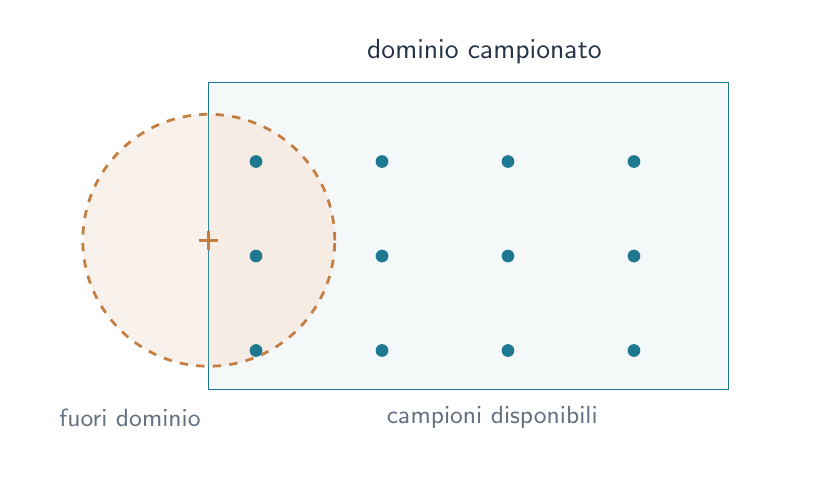
\begin{tikzpicture}[x=1cm,y=1cm]
\path[use as bounding box](-.1,-.15) rectangle(9.7,5.3);
\fill[GeoB!10](2.2,2.6)circle(1.6);
\filldraw[fill=GeoA!5,draw=GeoA](2.2,.7)rectangle(8.8,4.6);
\begin{scope}
\clip(2.2,.7)rectangle(8.8,4.6);
\fill[GeoB!15](2.2,2.6)circle(1.6);
\end{scope}
\draw[GeoB,dashed,line width=1pt](2.2,2.6)circle(1.6);
\foreach \x in {2.8,4.4,6,7.6}
 \foreach \y in {1.2,2.4,3.6}{\fill[GeoA](\x,\y)circle(2.3pt);}
\draw[GeoB,line width=1pt](2.08,2.6)--(2.32,2.6);
\draw[GeoB,line width=1pt](2.2,2.48)--(2.2,2.72);
\node[pLabel]at(5.7,5.0){dominio campionato};
\node[pNote]at(1.2,.35){fuori dominio};
\node[pNote]at(5.8,.35){campioni disponibili};

\end{tikzpicture}
\PInfo{Il supporto desiderato e il dominio campionato possono non coincidere. Al bordo del dominio parte del vicinato può essere priva di osservazioni.}

\end{minipage}\end{lrbox}
\typeout{FULLBOX:041:PilotLeftBox:\the\ht\PilotLeftBox:\the\dp\PilotLeftBox}

\begin{lrbox}{\PilotRightBox}
\begin{minipage}[t]{7.55cm}\raggedright\color{Ink}\fontsize{11.3}{14.8}\selectfont
\PBody{La mancanza di siti oltre il bordo non dimostra che il fenomeno si arresti lì. Può dipendere soltanto dall’estensione del rilievo.}
\vspace{2.5mm}
\PBody{Quando confrontiamo medie locali, registriamo quanti siti sono disponibili e come sono distribuiti rispetto al centro.}
\vspace{2.5mm}
\PSmall{Eventuali correzioni di bordo richiedono un modello o un disegno appropriato; non si ottengono aggiungendo valori non osservati.}

\end{minipage}\end{lrbox}
\typeout{FULLBOX:041:PilotRightBox:\the\ht\PilotRightBox:\the\dp\PilotRightBox}

\begin{tikzpicture}[remember picture,overlay]
\PilotChrome{Un buffer al bordo osserva una parte del disco}{III · CARTE E APPARTENENZE}{41}{Il confine del campionamento limita l’informazione disponibile sul vicinato.}
\node[anchor=north west,inner sep=0] at([xshift=.96cm,yshift=-2.13cm]current page.north west){\usebox{\PilotLeftBox}};
\node[anchor=north west,inner sep=0] at([xshift=11.52cm,yshift=-2.13cm]current page.north west){\usebox{\PilotRightBox}};
\end{tikzpicture}\end{frame}

\begin{frame}[plain]\hypertarget{slide42}{}
\bookmark[level=1,page=42]{Il disegno grafico non aggiunge osservazioni}
\begin{lrbox}{\TitleBox}
\begin{minipage}[t]{17.7cm}\raggedright\color{Ink}\fontsize{11.3}{14.8}\selectfont
\color{Navy}\bfseries\fontsize{20.6}{24.5}\selectfont Il disegno grafico non aggiunge osservazioni
\end{minipage}\end{lrbox}
\typeout{FULLBOX:042:TitleBox:\the\ht\TitleBox:\the\dp\TitleBox}

\begin{lrbox}{\RecallBox}
\begin{minipage}[t]{14.3cm}\raggedright\color{Ink}\fontsize{11.3}{14.8}\selectfont
\fontsize{10.3}{13.8}\selectfont La risoluzione della figura e la risoluzione dell’informazione osservata sono proprietà differenti.
\end{minipage}\end{lrbox}
\typeout{FULLBOX:042:RecallBox:\the\ht\RecallBox:\the\dp\RecallBox}

\begin{lrbox}{\PilotLeftBox}
\begin{minipage}[t]{10.05cm}\raggedright\color{Ink}\fontsize{11.3}{14.8}\selectfont
{\fontsize{10.2}{13.1}\selectfont\renewcommand{\arraystretch}{1.45}\begin{tabular}{@{}p{4.2cm}p{4.8cm}@{}}\toprule
\textbf{Operazione} & \textbf{Che cosa produce}\\\midrule
Disegnare un punto & Rappresentazione di un campione\\
Colorare un poligono con una media & Riassunto di campioni assegnati\\
Raffinare una griglia grafica & Più posizioni di visualizzazione\\
Interpolare sulla griglia & Previsioni dipendenti da una regola\\
\bottomrule\end{tabular}}

\end{minipage}\end{lrbox}
\typeout{FULLBOX:042:PilotLeftBox:\the\ht\PilotLeftBox:\the\dp\PilotLeftBox}

\begin{lrbox}{\PilotRightBox}
\begin{minipage}[t]{7.55cm}\raggedright\color{Ink}\fontsize{11.3}{14.8}\selectfont
\PBody{Una carta più liscia può facilitare la lettura, ma non aumenta il numero di misure disponibili. Le incertezze non scompaiono tra due pixel.}
\vspace{2.5mm}
\PInfo{Nel modulo la griglia di interpolazione contiene 45 punti per asse. I 2025 valori rappresentati sono previsioni ottenute dai 64 campioni.}
\PBody{Se una superficie copre aree lontane dai campioni, la legenda e il commento devono rendere esplicito questo limite.}
\vspace{2.5mm}

\end{minipage}\end{lrbox}
\typeout{FULLBOX:042:PilotRightBox:\the\ht\PilotRightBox:\the\dp\PilotRightBox}

\begin{tikzpicture}[remember picture,overlay]
\PilotChrome{Il disegno grafico non aggiunge osservazioni}{III · CARTE E APPARTENENZE}{42}{La risoluzione della figura e la risoluzione dell’informazione osservata sono proprietà differenti.}
\node[anchor=north west,inner sep=0] at([xshift=.96cm,yshift=-2.13cm]current page.north west){\usebox{\PilotLeftBox}};
\node[anchor=north west,inner sep=0] at([xshift=11.52cm,yshift=-2.13cm]current page.north west){\usebox{\PilotRightBox}};
\end{tikzpicture}\end{frame}

\begin{frame}[plain]\hypertarget{slide43}{}
\bookmark[level=1,page=43]{Laboratorio: carte e appartenenze verificabili}
\begin{lrbox}{\TitleBox}
\begin{minipage}[t]{17.7cm}\raggedright\color{Ink}\fontsize{11.3}{14.8}\selectfont
\color{Navy}\bfseries\fontsize{20.6}{24.5}\selectfont Laboratorio: carte e appartenenze verificabili
\end{minipage}\end{lrbox}
\typeout{FULLBOX:043:TitleBox:\the\ht\TitleBox:\the\dp\TitleBox}

\begin{lrbox}{\RecallBox}
\begin{minipage}[t]{14.3cm}\raggedright\color{Ink}\fontsize{11.3}{14.8}\selectfont
\fontsize{10.3}{13.8}\selectfont Ogni aggregazione deve rendere controllabile il passaggio dalle osservazioni alle unità di sintesi.
\end{minipage}\end{lrbox}
\typeout{FULLBOX:043:RecallBox:\the\ht\RecallBox:\the\dp\RecallBox}

\begin{lrbox}{\PilotLeftBox}
\begin{minipage}[t]{10.05cm}\raggedright\color{Ink}\fontsize{11.3}{14.8}\selectfont
\PLab{https://marzione00.github.io/Lab_Geo/\#laboratorio/m11-aggregazione}{Esperimento online · aggregazioni e confini}
{\fontsize{10.2}{13.1}\selectfont\renewcommand{\arraystretch}{1.45}\begin{tabular}{@{}p{4.0cm}p{5.0cm}@{}}\toprule
\textbf{Notebook} & \textbf{Domanda di controllo}\\\midrule
N07: punti & Dove sono le misure?\\
N08: partizione & Ogni ID compare in una sola area?\\
N09: sovrapposizione & Quanti ID hanno più appartenenze?\\
N10: buffer & Come cambiano conteggio e media?\\
\bottomrule\end{tabular}}

\end{minipage}\end{lrbox}
\typeout{FULLBOX:043:PilotLeftBox:\the\ht\PilotLeftBox:\the\dp\PilotLeftBox}

\begin{lrbox}{\PilotRightBox}
\begin{minipage}[t]{7.55cm}\raggedright\color{Ink}\fontsize{11.3}{14.8}\selectfont
\PBody{Per ogni operazione conservare tabella iniziale, regola geometrica e riepilogo dei conteggi. Un grafico senza questi elementi non basta a ricostruire il risultato.}
\vspace{2.5mm}
\PInfo{Una moltiplicazione delle righe può essere corretta. L’errore nasce quando cambia il peso statistico dei siti senza dichiararlo.}
\PBody{Il passo successivo assegna pesi direttamente alle coppie di siti.}
\vspace{2.5mm}

\end{minipage}\end{lrbox}
\typeout{FULLBOX:043:PilotRightBox:\the\ht\PilotRightBox:\the\dp\PilotRightBox}

\begin{tikzpicture}[remember picture,overlay]
\PilotChrome{Laboratorio: carte e appartenenze verificabili}{III · CARTE E APPARTENENZE}{43}{Ogni aggregazione deve rendere controllabile il passaggio dalle osservazioni alle unità di sintesi.}
\node[anchor=north west,inner sep=0] at([xshift=.96cm,yshift=-2.13cm]current page.north west){\usebox{\PilotLeftBox}};
\node[anchor=north west,inner sep=0] at([xshift=11.52cm,yshift=-2.13cm]current page.north west){\usebox{\PilotRightBox}};
\node[anchor=north east,inner sep=0] at([xshift=17.65cm,yshift=-12.06cm]current page.north west){\color{Classical}\fontsize{7.7}{9.2}\selectfont\href{../../03_Notebook_svolti/M11_Locus/M11_N09.html}{M11\_N09 · notebook svolto}};
\end{tikzpicture}\end{frame}

\begin{frame}[plain]\hypertarget{slide44}{}
\bookmark[level=0,page=44]{IV · VICINATI E PESI}
\bookmark[level=1,page=44]{Il vicinato è una scelta del modello}
\begin{lrbox}{\TitleBox}
\begin{minipage}[t]{17.7cm}\raggedright\color{Ink}\fontsize{11.3}{14.8}\selectfont
\color{Navy}\bfseries\fontsize{20.6}{24.5}\selectfont Il vicinato è una scelta del modello
\end{minipage}\end{lrbox}
\typeout{FULLBOX:044:TitleBox:\the\ht\TitleBox:\the\dp\TitleBox}

\begin{lrbox}{\RecallBox}
\begin{minipage}[t]{14.3cm}\raggedright\color{Ink}\fontsize{11.3}{14.8}\selectfont
\fontsize{10.3}{13.8}\selectfont Il significato di vicino deve essere esplicito prima del calcolo dei pesi.
\end{minipage}\end{lrbox}
\typeout{FULLBOX:044:RecallBox:\the\ht\RecallBox:\the\dp\RecallBox}

\begin{lrbox}{\PilotLeftBox}
\begin{minipage}[t]{10.05cm}\raggedright\color{Ink}\fontsize{11.3}{14.8}\selectfont
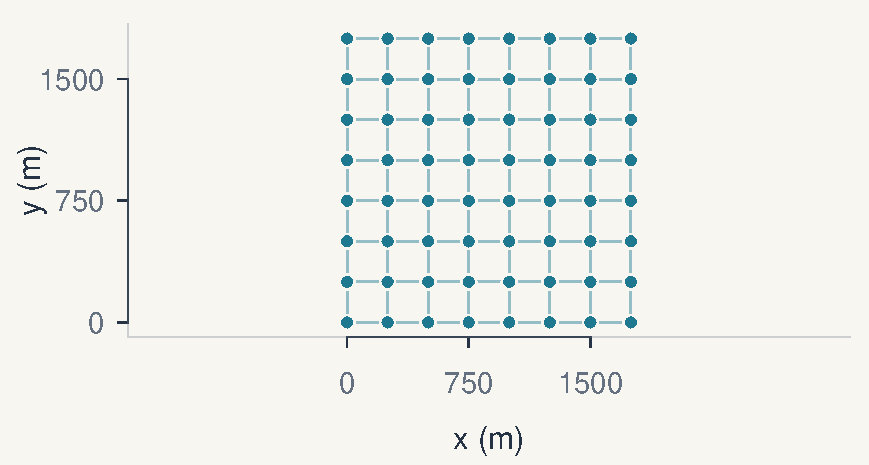
\includegraphics[width=9.85cm,height=5.25cm,keepaspectratio]{Risultati/Figure/13_vicini_soglia.pdf}
\vspace{1.5mm}
\PSmall{Una soglia di 260 m collega i vicini ortogonali della griglia; le diagonali restano escluse.}

\end{minipage}\end{lrbox}
\typeout{FULLBOX:044:PilotLeftBox:\the\ht\PilotLeftBox:\the\dp\PilotLeftBox}

\begin{lrbox}{\PilotRightBox}
\begin{minipage}[t]{7.55cm}\raggedright\color{Ink}\fontsize{11.3}{14.8}\selectfont
\PBody{Definiamo vicini i siti distinti con distanza non superiore a 260 m. La soglia supera il passo di 250 m ed è inferiore alla diagonale di circa 354 m.}
\vspace{2.5mm}
\PInfo{Il grafo così costruito contiene 112 archi non orientati. La matrice simmetrica registra ciascun arco in due celle.}
\PBody{Soglia e metrica vengono fissate prima di misurare l’associazione.}
\vspace{2.5mm}

\end{minipage}\end{lrbox}
\typeout{FULLBOX:044:PilotRightBox:\the\ht\PilotRightBox:\the\dp\PilotRightBox}

\begin{tikzpicture}[remember picture,overlay]
\PilotChrome{Il vicinato è una scelta del modello}{IV · VICINATI E PESI}{44}{Il significato di vicino deve essere esplicito prima del calcolo dei pesi.}
\node[anchor=north west,inner sep=0] at([xshift=.96cm,yshift=-2.13cm]current page.north west){\usebox{\PilotLeftBox}};
\node[anchor=north west,inner sep=0] at([xshift=11.52cm,yshift=-2.13cm]current page.north west){\usebox{\PilotRightBox}};
\end{tikzpicture}\end{frame}

\begin{frame}[plain]\hypertarget{slide45}{}
\bookmark[level=1,page=45]{Una soglia può generare vicinati diversi}
\begin{lrbox}{\TitleBox}
\begin{minipage}[t]{17.7cm}\raggedright\color{Ink}\fontsize{11.3}{14.8}\selectfont
\color{Navy}\bfseries\fontsize{20.6}{24.5}\selectfont Una soglia può generare vicinati diversi
\end{minipage}\end{lrbox}
\typeout{FULLBOX:045:TitleBox:\the\ht\TitleBox:\the\dp\TitleBox}

\begin{lrbox}{\RecallBox}
\begin{minipage}[t]{14.3cm}\raggedright\color{Ink}\fontsize{11.3}{14.8}\selectfont
\fontsize{10.3}{13.8}\selectfont Cambiare soglia cambia il grafo e quindi il fenomeno di associazione che si misura.
\end{minipage}\end{lrbox}
\typeout{FULLBOX:045:RecallBox:\the\ht\RecallBox:\the\dp\RecallBox}

\begin{lrbox}{\PilotLeftBox}
\begin{minipage}[t]{10.05cm}\raggedright\color{Ink}\fontsize{11.3}{14.8}\selectfont
\[A_{ij}=\mathbf1(0<d_{ij}\le r),\qquad A_{ii}=0\]
{\fontsize{10.2}{13.1}\selectfont\renewcommand{\arraystretch}{1.45}\begin{tabular}{@{}p{4.5cm}p{4.5cm}@{}}\toprule
\textbf{Soglia sulla griglia} & \textbf{Conseguenza}\\\midrule
$r<250$ m & Nessun vicino distinto\\
$250\le r<250\sqrt2$ m & Vicini ortogonali\\
$r\ge250\sqrt2$ m & Entrano anche le diagonali vicine\\
Soglia molto grande & La relazione diventa meno locale\\
\bottomrule\end{tabular}}

\end{minipage}\end{lrbox}
\typeout{FULLBOX:045:PilotLeftBox:\the\ht\PilotLeftBox:\the\dp\PilotLeftBox}

\begin{lrbox}{\PilotRightBox}
\begin{minipage}[t]{7.55cm}\raggedright\color{Ink}\fontsize{11.3}{14.8}\selectfont
\PBody{La disuguaglianza sul bordo della soglia fa parte della definizione. Con distanze calcolate numericamente, la tolleranza va motivata se necessaria.}
\vspace{2.5mm}
\PInfo{Nelle coordinate locali del caso guida la soglia di 260 m evita ambiguità sul passo di 250 m.}
\PCode{R · adiacenza binaria}{045_esempio.R}
\end{minipage}\end{lrbox}
\typeout{FULLBOX:045:PilotRightBox:\the\ht\PilotRightBox:\the\dp\PilotRightBox}

\begin{tikzpicture}[remember picture,overlay]
\PilotChrome{Una soglia può generare vicinati diversi}{IV · VICINATI E PESI}{45}{Cambiare soglia cambia il grafo e quindi il fenomeno di associazione che si misura.}
\node[anchor=north west,inner sep=0] at([xshift=.96cm,yshift=-2.13cm]current page.north west){\usebox{\PilotLeftBox}};
\node[anchor=north west,inner sep=0] at([xshift=11.52cm,yshift=-2.13cm]current page.north west){\usebox{\PilotRightBox}};
\node[anchor=north east,inner sep=0] at([xshift=17.65cm,yshift=-12.06cm]current page.north west){\color{Classical}\fontsize{7.7}{9.2}\selectfont\href{../../03_Notebook_svolti/M11_Locus/M11_N12.html}{M11\_N12 · notebook svolto}};
\end{tikzpicture}\end{frame}

\begin{frame}[plain]\hypertarget{slide46}{}
\bookmark[level=1,page=46]{Vicino più prossimo: esclusione e parità}
\begin{lrbox}{\TitleBox}
\begin{minipage}[t]{17.7cm}\raggedright\color{Ink}\fontsize{11.3}{14.8}\selectfont
\color{Navy}\bfseries\fontsize{20.6}{24.5}\selectfont Vicino più prossimo: esclusione e parità
\end{minipage}\end{lrbox}
\typeout{FULLBOX:046:TitleBox:\the\ht\TitleBox:\the\dp\TitleBox}

\begin{lrbox}{\RecallBox}
\begin{minipage}[t]{14.3cm}\raggedright\color{Ink}\fontsize{11.3}{14.8}\selectfont
\fontsize{10.3}{13.8}\selectfont Il vicino più prossimo richiede una regola per l’autocoincidenza e una per le distanze uguali.
\end{minipage}\end{lrbox}
\typeout{FULLBOX:046:RecallBox:\the\ht\RecallBox:\the\dp\RecallBox}

\begin{lrbox}{\PilotLeftBox}
\begin{minipage}[t]{10.05cm}\raggedright\color{Ink}\fontsize{11.3}{14.8}\selectfont
\[j^\star(i)\in\arg\min_{j\ne i}d_{ij}\]
\PInfo{Sulla griglia diversi siti sono alla stessa distanza minima. Il laboratorio risolve le parità scegliendo il primo indice nell’ordine degli ID.}

\end{minipage}\end{lrbox}
\typeout{FULLBOX:046:PilotLeftBox:\the\ht\PilotLeftBox:\the\dp\PilotLeftBox}

\begin{lrbox}{\PilotRightBox}
\begin{minipage}[t]{7.55cm}\raggedright\color{Ink}\fontsize{11.3}{14.8}\selectfont
\PBody{Se non si esclude la diagonale, il vicino più prossimo di ogni sito è il sito stesso. Per evitarlo sostituiamo la diagonale con infinito solo nella matrice di ricerca.}
\vspace{2.5mm}
\PBody{La regola delle parità è riproducibile ma non aggiunge una preferenza fisica. Se serve includere tutti gli ex aequo, cambia la struttura del vicinato.}
\vspace{2.5mm}
\PCode{R · escludere il sito stesso}{046_esempio.R}
\end{minipage}\end{lrbox}
\typeout{FULLBOX:046:PilotRightBox:\the\ht\PilotRightBox:\the\dp\PilotRightBox}

\begin{tikzpicture}[remember picture,overlay]
\PilotChrome{Vicino più prossimo: esclusione e parità}{IV · VICINATI E PESI}{46}{Il vicino più prossimo richiede una regola per l’autocoincidenza e una per le distanze uguali.}
\node[anchor=north west,inner sep=0] at([xshift=.96cm,yshift=-2.13cm]current page.north west){\usebox{\PilotLeftBox}};
\node[anchor=north west,inner sep=0] at([xshift=11.52cm,yshift=-2.13cm]current page.north west){\usebox{\PilotRightBox}};
\node[anchor=north east,inner sep=0] at([xshift=17.65cm,yshift=-12.06cm]current page.north west){\color{Classical}\fontsize{7.7}{9.2}\selectfont\href{../../03_Notebook_svolti/M11_Locus/M11_N11.html}{M11\_N11 · notebook svolto}};
\end{tikzpicture}\end{frame}

\begin{frame}[plain]\hypertarget{slide47}{}
\bookmark[level=1,page=47]{Il grado conta quanti vicini ha un sito}
\begin{lrbox}{\TitleBox}
\begin{minipage}[t]{17.7cm}\raggedright\color{Ink}\fontsize{11.3}{14.8}\selectfont
\color{Navy}\bfseries\fontsize{20.6}{24.5}\selectfont Il grado conta quanti vicini ha un sito
\end{minipage}\end{lrbox}
\typeout{FULLBOX:047:TitleBox:\the\ht\TitleBox:\the\dp\TitleBox}

\begin{lrbox}{\RecallBox}
\begin{minipage}[t]{14.3cm}\raggedright\color{Ink}\fontsize{11.3}{14.8}\selectfont
\fontsize{10.3}{13.8}\selectfont Il grado distingue la struttura del vicinato dal valore misurato nel sito.
\end{minipage}\end{lrbox}
\typeout{FULLBOX:047:RecallBox:\the\ht\RecallBox:\the\dp\RecallBox}

\begin{lrbox}{\PilotLeftBox}
\begin{minipage}[t]{10.05cm}\raggedright\color{Ink}\fontsize{11.3}{14.8}\selectfont
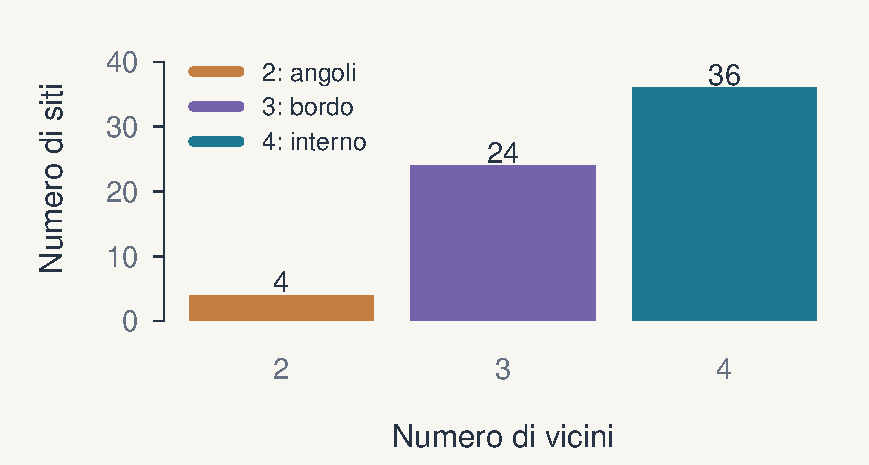
\includegraphics[width=9.85cm,height=5.25cm,keepaspectratio]{Risultati/Figure/14_gradi_vicinato.pdf}
\vspace{1.5mm}
\PSmall{Con vicinato ortogonale: 4 angoli con grado 2, 24 bordi con grado 3, 36 interni con grado 4.}

\end{minipage}\end{lrbox}
\typeout{FULLBOX:047:PilotLeftBox:\the\ht\PilotLeftBox:\the\dp\PilotLeftBox}

\begin{lrbox}{\PilotRightBox}
\begin{minipage}[t]{7.55cm}\raggedright\color{Ink}\fontsize{11.3}{14.8}\selectfont
\PBody{La somma di una riga di A è il grado del sito. I punti al bordo hanno meno collegamenti disponibili.}
\vspace{2.5mm}
\PInfo{La somma dei gradi è 224, cioè due volte il numero degli archi non orientati. Questo conteggio verifica la costruzione del grafo.}
\PCode{R · contare i collegamenti}{047_esempio.R}
\end{minipage}\end{lrbox}
\typeout{FULLBOX:047:PilotRightBox:\the\ht\PilotRightBox:\the\dp\PilotRightBox}

\begin{tikzpicture}[remember picture,overlay]
\PilotChrome{Il grado conta quanti vicini ha un sito}{IV · VICINATI E PESI}{47}{Il grado distingue la struttura del vicinato dal valore misurato nel sito.}
\node[anchor=north west,inner sep=0] at([xshift=.96cm,yshift=-2.13cm]current page.north west){\usebox{\PilotLeftBox}};
\node[anchor=north west,inner sep=0] at([xshift=11.52cm,yshift=-2.13cm]current page.north west){\usebox{\PilotRightBox}};
\node[anchor=north east,inner sep=0] at([xshift=17.65cm,yshift=-12.06cm]current page.north west){\color{Classical}\fontsize{7.7}{9.2}\selectfont\href{../../03_Notebook_svolti/M11_Locus/M11_N12.html}{M11\_N12 · notebook svolto}};
\end{tikzpicture}\end{frame}

\begin{frame}[plain]\hypertarget{slide48}{}
\bookmark[level=1,page=48]{Normalizzare per riga costruisce una media}
\begin{lrbox}{\TitleBox}
\begin{minipage}[t]{17.7cm}\raggedright\color{Ink}\fontsize{11.3}{14.8}\selectfont
\color{Navy}\bfseries\fontsize{20.6}{24.5}\selectfont Normalizzare per riga costruisce una media
\end{minipage}\end{lrbox}
\typeout{FULLBOX:048:TitleBox:\the\ht\TitleBox:\the\dp\TitleBox}

\begin{lrbox}{\RecallBox}
\begin{minipage}[t]{14.3cm}\raggedright\color{Ink}\fontsize{11.3}{14.8}\selectfont
\fontsize{10.3}{13.8}\selectfont La normalizzazione per riga cambia il significato dei pesi e del ritardo spaziale.
\end{minipage}\end{lrbox}
\typeout{FULLBOX:048:RecallBox:\the\ht\RecallBox:\the\dp\RecallBox}

\begin{lrbox}{\PilotLeftBox}
\begin{minipage}[t]{10.05cm}\raggedright\color{Ink}\fontsize{11.3}{14.8}\selectfont
\begin{tikzpicture}[x=1cm,y=1cm]
\path[use as bounding box](-.1,-.15) rectangle(9.7,5.3);
\node[pFlow,fill=GeoB!10,text width=1.6cm](s)at(4.7,2.6){$s_i$};
\node[pFlow,fill=GeoA!8,text width=1.6cm](a)at(1.1,2.6){$s_1$};
\node[pFlow,fill=GeoA!8,text width=1.6cm](b)at(8.3,2.6){$s_2$};
\node[pFlow,fill=GeoA!8,text width=1.6cm](c)at(4.7,4.65){$s_3$};
\node[pFlow,fill=GeoA!8,text width=1.6cm](d)at(4.7,.6){$s_4$};
\draw[pEdge](a)--node[above,pNote]{$1/4$}(s);
\draw[pEdge](b)--node[above,pNote]{$1/4$}(s);
\draw[pEdge](c)--node[right,pNote]{$1/4$}(s);
\draw[pEdge](d)--node[right,pNote]{$1/4$}(s);
\end{tikzpicture}
\[W_{ij}=\frac{A_{ij}}{\sum_k A_{ik}},\qquad \sum_jW_{ij}=1\]

\end{minipage}\end{lrbox}
\typeout{FULLBOX:048:PilotLeftBox:\the\ht\PilotLeftBox:\the\dp\PilotLeftBox}

\begin{lrbox}{\PilotRightBox}
\begin{minipage}[t]{7.55cm}\raggedright\color{Ink}\fontsize{11.3}{14.8}\selectfont
\PBody{Per un sito con quattro vicini ogni peso è $1/4$. Per un angolo con due vicini ogni peso è $1/2$.}
\vspace{2.5mm}
\PInfo{La normalizzazione rende il ritardo spaziale una media dei vicini. Non elimina la differenza nella copertura geometrica fra centro e bordo.}
\PCode{R · pesi normalizzati}{048_esempio.R}
\end{minipage}\end{lrbox}
\typeout{FULLBOX:048:PilotRightBox:\the\ht\PilotRightBox:\the\dp\PilotRightBox}

\begin{tikzpicture}[remember picture,overlay]
\PilotChrome{Normalizzare per riga costruisce una media}{IV · VICINATI E PESI}{48}{La normalizzazione per riga cambia il significato dei pesi e del ritardo spaziale.}
\node[anchor=north west,inner sep=0] at([xshift=.96cm,yshift=-2.13cm]current page.north west){\usebox{\PilotLeftBox}};
\node[anchor=north west,inner sep=0] at([xshift=11.52cm,yshift=-2.13cm]current page.north west){\usebox{\PilotRightBox}};
\node[anchor=north east,inner sep=0] at([xshift=17.65cm,yshift=-12.06cm]current page.north west){\color{Classical}\fontsize{7.7}{9.2}\selectfont\href{../../03_Notebook_svolti/M11_Locus/M11_N12.html}{M11\_N12 · notebook svolto}};
\end{tikzpicture}\end{frame}

\begin{frame}[plain]\hypertarget{slide49}{}
\bookmark[level=1,page=49]{Da A a W: stessa rete, pesi differenti}
\begin{lrbox}{\TitleBox}
\begin{minipage}[t]{17.7cm}\raggedright\color{Ink}\fontsize{11.3}{14.8}\selectfont
\color{Navy}\bfseries\fontsize{20.6}{24.5}\selectfont Da A a W: stessa rete, pesi differenti
\end{minipage}\end{lrbox}
\typeout{FULLBOX:049:TitleBox:\the\ht\TitleBox:\the\dp\TitleBox}

\begin{lrbox}{\RecallBox}
\begin{minipage}[t]{14.3cm}\raggedright\color{Ink}\fontsize{11.3}{14.8}\selectfont
\fontsize{10.3}{13.8}\selectfont La simmetria dell’adiacenza non garantisce la simmetria dei pesi normalizzati.
\end{minipage}\end{lrbox}
\typeout{FULLBOX:049:RecallBox:\the\ht\RecallBox:\the\dp\RecallBox}

\begin{lrbox}{\PilotLeftBox}
\begin{minipage}[t]{10.05cm}\raggedright\color{Ink}\fontsize{11.3}{14.8}\selectfont
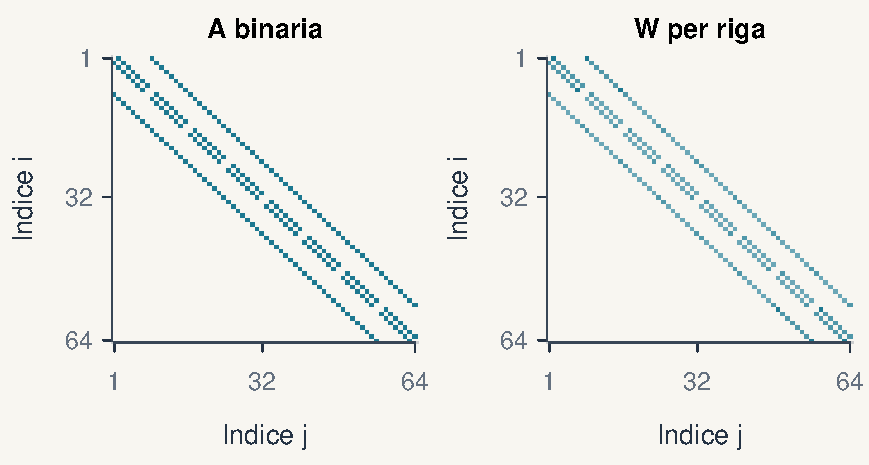
\includegraphics[width=9.85cm,height=5.25cm,keepaspectratio]{Risultati/Figure/15_matrici_A_W.pdf}
\vspace{1.5mm}
\PSmall{Le celle non nulle sono le stesse. La normalizzazione per riga modifica le intensità.}

\end{minipage}\end{lrbox}
\typeout{FULLBOX:049:PilotLeftBox:\the\ht\PilotLeftBox:\the\dp\PilotLeftBox}

\begin{lrbox}{\PilotRightBox}
\begin{minipage}[t]{7.55cm}\raggedright\color{Ink}\fontsize{11.3}{14.8}\selectfont
\PBody{A è simmetrica perché la distanza lo è. W può essere asimmetrica: un angolo assegna $1/2$ a un vicino che gli assegna $1/3$.}
\vspace{2.5mm}
\PInfo{Due statistiche calcolate con A e W non devono essere interpretate come lo stesso risultato. Il nome “Moran I” richiede di specificare anche i pesi.}
\PCode{R · distinguere le matrici}{049_esempio.R}
\end{minipage}\end{lrbox}
\typeout{FULLBOX:049:PilotRightBox:\the\ht\PilotRightBox:\the\dp\PilotRightBox}

\begin{tikzpicture}[remember picture,overlay]
\PilotChrome{Da A a W: stessa rete, pesi differenti}{IV · VICINATI E PESI}{49}{La simmetria dell’adiacenza non garantisce la simmetria dei pesi normalizzati.}
\node[anchor=north west,inner sep=0] at([xshift=.96cm,yshift=-2.13cm]current page.north west){\usebox{\PilotLeftBox}};
\node[anchor=north west,inner sep=0] at([xshift=11.52cm,yshift=-2.13cm]current page.north west){\usebox{\PilotRightBox}};
\node[anchor=north east,inner sep=0] at([xshift=17.65cm,yshift=-12.06cm]current page.north west){\color{Classical}\fontsize{7.7}{9.2}\selectfont\href{../../03_Notebook_svolti/M11_Locus/M11_N12.html}{M11\_N12 · notebook svolto}};
\end{tikzpicture}\end{frame}

\begin{frame}[plain]\hypertarget{slide50}{}
\bookmark[level=1,page=50]{Un sito isolato richiede una regola esplicita}
\begin{lrbox}{\TitleBox}
\begin{minipage}[t]{17.7cm}\raggedright\color{Ink}\fontsize{11.3}{14.8}\selectfont
\color{Navy}\bfseries\fontsize{20.6}{24.5}\selectfont Un sito isolato richiede una regola esplicita
\end{minipage}\end{lrbox}
\typeout{FULLBOX:050:TitleBox:\the\ht\TitleBox:\the\dp\TitleBox}

\begin{lrbox}{\RecallBox}
\begin{minipage}[t]{14.3cm}\raggedright\color{Ink}\fontsize{11.3}{14.8}\selectfont
\fontsize{10.3}{13.8}\selectfont Il trattamento degli isolati entra nella definizione della statistica e del campione.
\end{minipage}\end{lrbox}
\typeout{FULLBOX:050:RecallBox:\the\ht\RecallBox:\the\dp\RecallBox}

\begin{lrbox}{\PilotLeftBox}
\begin{minipage}[t]{10.05cm}\raggedright\color{Ink}\fontsize{11.3}{14.8}\selectfont
\[\sum_jA_{ij}=0\quad\Longrightarrow\quad A_{ij}/0\ \text{non definito}\]
{\fontsize{10.2}{13.1}\selectfont\renewcommand{\arraystretch}{1.45}\begin{tabular}{@{}p{4.1cm}p{4.9cm}@{}}\toprule
\textbf{Possibile scelta} & \textbf{Conseguenza da dichiarare}\\\midrule
Rivedere il vicinato & Cambia la relazione analizzata\\
Escludere il sito & Cambia il campione e può creare altri isolati\\
Assegnare ritardo zero & È una convenzione del metodo\\
Lasciare il valore mancante & Richiede un’analisi coerente dei mancanti\\
\bottomrule\end{tabular}}

\end{minipage}\end{lrbox}
\typeout{FULLBOX:050:PilotLeftBox:\the\ht\PilotLeftBox:\the\dp\PilotLeftBox}

\begin{lrbox}{\PilotRightBox}
\begin{minipage}[t]{7.55cm}\raggedright\color{Ink}\fontsize{11.3}{14.8}\selectfont
\PBody{Con la soglia principale ogni sito ha almeno due vicini. Questo fatto viene controllato prima di normalizzare.}
\vspace{2.5mm}
\PInfo{Con 200 m tutti i siti sarebbero isolati. Una divisione silenziosa per zero produrrebbe valori non validi.}
\PCode{R · un caso limite controllato}{050_esempio.R}
\end{minipage}\end{lrbox}
\typeout{FULLBOX:050:PilotRightBox:\the\ht\PilotRightBox:\the\dp\PilotRightBox}

\begin{tikzpicture}[remember picture,overlay]
\PilotChrome{Un sito isolato richiede una regola esplicita}{IV · VICINATI E PESI}{50}{Il trattamento degli isolati entra nella definizione della statistica e del campione.}
\node[anchor=north west,inner sep=0] at([xshift=.96cm,yshift=-2.13cm]current page.north west){\usebox{\PilotLeftBox}};
\node[anchor=north west,inner sep=0] at([xshift=11.52cm,yshift=-2.13cm]current page.north west){\usebox{\PilotRightBox}};
\node[anchor=north east,inner sep=0] at([xshift=17.65cm,yshift=-12.06cm]current page.north west){\color{Classical}\fontsize{7.7}{9.2}\selectfont\href{../../03_Notebook_svolti/M11_Locus/M11_N12.html}{M11\_N12 · notebook svolto}};
\end{tikzpicture}\end{frame}

\begin{frame}[plain]\hypertarget{slide51}{}
\bookmark[level=1,page=51]{Il ritardo spaziale riassume i vicini}
\begin{lrbox}{\TitleBox}
\begin{minipage}[t]{17.7cm}\raggedright\color{Ink}\fontsize{11.3}{14.8}\selectfont
\color{Navy}\bfseries\fontsize{20.6}{24.5}\selectfont Il ritardo spaziale riassume i vicini
\end{minipage}\end{lrbox}
\typeout{FULLBOX:051:TitleBox:\the\ht\TitleBox:\the\dp\TitleBox}

\begin{lrbox}{\RecallBox}
\begin{minipage}[t]{14.3cm}\raggedright\color{Ink}\fontsize{11.3}{14.8}\selectfont
\fontsize{10.3}{13.8}\selectfont Il ritardo spaziale dipende dai valori dei vicini e dalla regola con cui sono pesati.
\end{minipage}\end{lrbox}
\typeout{FULLBOX:051:RecallBox:\the\ht\RecallBox:\the\dp\RecallBox}

\begin{lrbox}{\PilotLeftBox}
\begin{minipage}[t]{10.05cm}\raggedright\color{Ink}\fontsize{11.3}{14.8}\selectfont
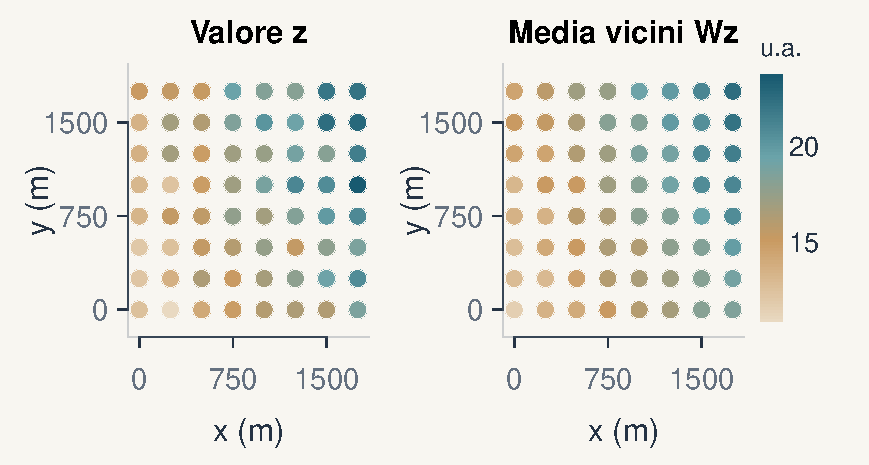
\includegraphics[width=9.85cm,height=5.25cm,keepaspectratio]{Risultati/Figure/16_lag_spaziale.pdf}
\vspace{1.5mm}
\PSmall{Valore nel sito e media dei vicini sono quantità diverse, calcolate con gli stessi ID.}
\[(Wz)_i=\sum_jW_{ij}z_j\]

\end{minipage}\end{lrbox}
\typeout{FULLBOX:051:PilotLeftBox:\the\ht\PilotLeftBox:\the\dp\PilotLeftBox}

\begin{lrbox}{\PilotRightBox}
\begin{minipage}[t]{7.55cm}\raggedright\color{Ink}\fontsize{11.3}{14.8}\selectfont
\PBody{Il ritardo spaziale non sposta i dati nel tempo. Costruisce per ogni sito una combinazione dei valori nei siti collegati.}
\vspace{2.5mm}
\PInfo{Con pesi non negativi normalizzati per riga, il risultato è una media. Se tutte le misure sono costanti, il ritardo riproduce quella costante.}
\PCode{R · media del vicinato}{051_esempio.R}
\end{minipage}\end{lrbox}
\typeout{FULLBOX:051:PilotRightBox:\the\ht\PilotRightBox:\the\dp\PilotRightBox}

\begin{tikzpicture}[remember picture,overlay]
\PilotChrome{Il ritardo spaziale riassume i vicini}{IV · VICINATI E PESI}{51}{Il ritardo spaziale dipende dai valori dei vicini e dalla regola con cui sono pesati.}
\node[anchor=north west,inner sep=0] at([xshift=.96cm,yshift=-2.13cm]current page.north west){\usebox{\PilotLeftBox}};
\node[anchor=north west,inner sep=0] at([xshift=11.52cm,yshift=-2.13cm]current page.north west){\usebox{\PilotRightBox}};
\node[anchor=north east,inner sep=0] at([xshift=17.65cm,yshift=-12.06cm]current page.north west){\color{Classical}\fontsize{7.7}{9.2}\selectfont\href{../../03_Notebook_svolti/M11_Locus/M11_N12.html}{M11\_N12 · notebook svolto}};
\end{tikzpicture}\end{frame}

\begin{frame}[plain]\hypertarget{slide52}{}
\bookmark[level=1,page=52]{Un riordinamento deve coinvolgere valori e pesi}
\begin{lrbox}{\TitleBox}
\begin{minipage}[t]{17.7cm}\raggedright\color{Ink}\fontsize{11.3}{14.8}\selectfont
\color{Navy}\bfseries\fontsize{20.6}{24.5}\selectfont Un riordinamento deve coinvolgere valori e pesi
\end{minipage}\end{lrbox}
\typeout{FULLBOX:052:TitleBox:\the\ht\TitleBox:\the\dp\TitleBox}

\begin{lrbox}{\RecallBox}
\begin{minipage}[t]{14.3cm}\raggedright\color{Ink}\fontsize{11.3}{14.8}\selectfont
\fontsize{10.3}{13.8}\selectfont La statistica deve restare invariata sotto un riordinamento coerente delle osservazioni.
\end{minipage}\end{lrbox}
\typeout{FULLBOX:052:RecallBox:\the\ht\RecallBox:\the\dp\RecallBox}

\begin{lrbox}{\PilotLeftBox}
\begin{minipage}[t]{10.05cm}\raggedright\color{Ink}\fontsize{11.3}{14.8}\selectfont
\[z^\star=Pz,\qquad W^\star=PWP^\top\]
\[W^\star z^\star=P(Wz)\]
\PInfo{$P$ è una matrice di permutazione. Cambiare ordine a tutte le componenti conserva il risultato associato ai singoli siti.}

\end{minipage}\end{lrbox}
\typeout{FULLBOX:052:PilotLeftBox:\the\ht\PilotLeftBox:\the\dp\PilotLeftBox}

\begin{lrbox}{\PilotRightBox}
\begin{minipage}[t]{7.55cm}\raggedright\color{Ink}\fontsize{11.3}{14.8}\selectfont
\PBody{Riordinare soltanto i valori distrugge la corrispondenza con le righe della matrice. Il codice resta eseguibile ma risponde a un’altra disposizione spaziale.}
\vspace{2.5mm}
\PBody{Il controllo per ID evita di usare la posizione nella tabella come identità del campione.}
\vspace{2.5mm}
\PCode{R · invarianza all’ordine}{052_esempio.R}
\end{minipage}\end{lrbox}
\typeout{FULLBOX:052:PilotRightBox:\the\ht\PilotRightBox:\the\dp\PilotRightBox}

\begin{tikzpicture}[remember picture,overlay]
\PilotChrome{Un riordinamento deve coinvolgere valori e pesi}{IV · VICINATI E PESI}{52}{La statistica deve restare invariata sotto un riordinamento coerente delle osservazioni.}
\node[anchor=north west,inner sep=0] at([xshift=.96cm,yshift=-2.13cm]current page.north west){\usebox{\PilotLeftBox}};
\node[anchor=north west,inner sep=0] at([xshift=11.52cm,yshift=-2.13cm]current page.north west){\usebox{\PilotRightBox}};
\node[anchor=north east,inner sep=0] at([xshift=17.65cm,yshift=-12.06cm]current page.north west){\color{Classical}\fontsize{7.7}{9.2}\selectfont\href{../../03_Notebook_svolti/M11_Locus/M11_N12.html}{M11\_N12 · notebook svolto}};
\end{tikzpicture}\end{frame}

\begin{frame}[plain]\hypertarget{slide53}{}
\bookmark[level=1,page=53]{Il bordo cambia la geometria del confronto}
\begin{lrbox}{\TitleBox}
\begin{minipage}[t]{17.7cm}\raggedright\color{Ink}\fontsize{11.3}{14.8}\selectfont
\color{Navy}\bfseries\fontsize{20.6}{24.5}\selectfont Il bordo cambia la geometria del confronto
\end{minipage}\end{lrbox}
\typeout{FULLBOX:053:TitleBox:\the\ht\TitleBox:\the\dp\TitleBox}

\begin{lrbox}{\RecallBox}
\begin{minipage}[t]{14.3cm}\raggedright\color{Ink}\fontsize{11.3}{14.8}\selectfont
\fontsize{10.3}{13.8}\selectfont Una somma dei pesi uguale a uno non implica uguale informazione spaziale.
\end{minipage}\end{lrbox}
\typeout{FULLBOX:053:RecallBox:\the\ht\RecallBox:\the\dp\RecallBox}

\begin{lrbox}{\PilotLeftBox}
\begin{minipage}[t]{10.05cm}\raggedright\color{Ink}\fontsize{11.3}{14.8}\selectfont
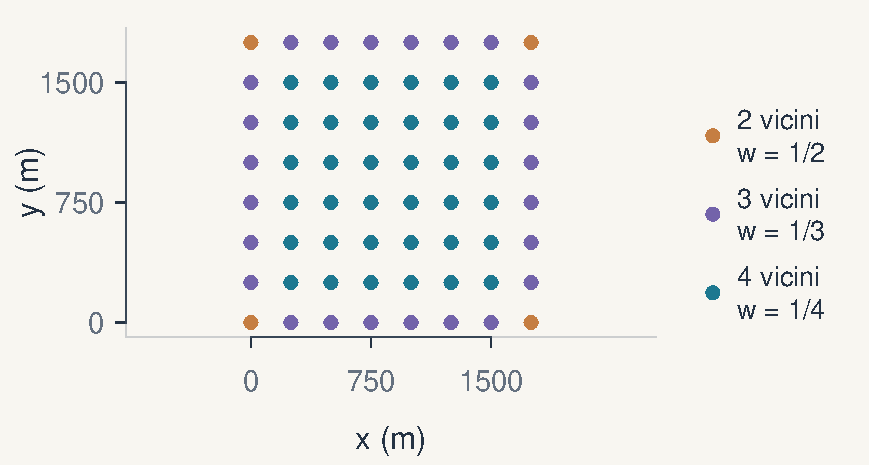
\includegraphics[width=9.85cm,height=5.25cm,keepaspectratio]{Risultati/Figure/17_effetti_bordo.pdf}
\vspace{1.5mm}
\PSmall{Centro, lato e angolo hanno disponibilità di vicini differenti, anche con pesi di riga unitari.}

\end{minipage}\end{lrbox}
\typeout{FULLBOX:053:PilotLeftBox:\the\ht\PilotLeftBox:\the\dp\PilotLeftBox}

\begin{lrbox}{\PilotRightBox}
\begin{minipage}[t]{7.55cm}\raggedright\color{Ink}\fontsize{11.3}{14.8}\selectfont
\PBody{La normalizzazione uniforma la somma dei pesi, ma non rende equivalenti il vicinato di un angolo e quello di un sito interno.}
\vspace{2.5mm}
\PInfo{Un sito al bordo confronta i valori osservati da un solo lato. Se il fenomeno ha un gradiente, questa asimmetria geometrica può incidere sul ritardo.}
\PBody{La diagnosi del vicinato deve quindi includere mappa, gradi e presenza di componenti separate.}
\vspace{2.5mm}

\end{minipage}\end{lrbox}
\typeout{FULLBOX:053:PilotRightBox:\the\ht\PilotRightBox:\the\dp\PilotRightBox}

\begin{tikzpicture}[remember picture,overlay]
\PilotChrome{Il bordo cambia la geometria del confronto}{IV · VICINATI E PESI}{53}{Una somma dei pesi uguale a uno non implica uguale informazione spaziale.}
\node[anchor=north west,inner sep=0] at([xshift=.96cm,yshift=-2.13cm]current page.north west){\usebox{\PilotLeftBox}};
\node[anchor=north west,inner sep=0] at([xshift=11.52cm,yshift=-2.13cm]current page.north west){\usebox{\PilotRightBox}};
\end{tikzpicture}\end{frame}

\begin{frame}[plain]\hypertarget{slide54}{}
\bookmark[level=1,page=54]{La sensibilità ai pesi fa parte del risultato}
\begin{lrbox}{\TitleBox}
\begin{minipage}[t]{17.7cm}\raggedright\color{Ink}\fontsize{11.3}{14.8}\selectfont
\color{Navy}\bfseries\fontsize{20.6}{24.5}\selectfont La sensibilità ai pesi fa parte del risultato
\end{minipage}\end{lrbox}
\typeout{FULLBOX:054:TitleBox:\the\ht\TitleBox:\the\dp\TitleBox}

\begin{lrbox}{\RecallBox}
\begin{minipage}[t]{14.3cm}\raggedright\color{Ink}\fontsize{11.3}{14.8}\selectfont
\fontsize{10.3}{13.8}\selectfont La robustezza rispetto ai pesi va studiata senza scegliere la sola configurazione favorevole.
\end{minipage}\end{lrbox}
\typeout{FULLBOX:054:RecallBox:\the\ht\RecallBox:\the\dp\RecallBox}

\begin{lrbox}{\PilotLeftBox}
\begin{minipage}[t]{10.05cm}\raggedright\color{Ink}\fontsize{11.3}{14.8}\selectfont
{\fontsize{10.2}{13.1}\selectfont\renewcommand{\arraystretch}{1.45}\begin{tabular}{@{}p{4.1cm}p{4.9cm}@{}}\toprule
\textbf{Modifica} & \textbf{Che cosa può cambiare}\\\midrule
Soglia di distanza & Scala della relazione\\
Numero fisso di vicini & Raggio locale variabile\\
Pesi binari o di riga & Contributo dei siti con gradi diversi\\
Distanza o rete & Nozione fisica di connessione\\
\bottomrule\end{tabular}}

\end{minipage}\end{lrbox}
\typeout{FULLBOX:054:PilotLeftBox:\the\ht\PilotLeftBox:\the\dp\PilotLeftBox}

\begin{lrbox}{\PilotRightBox}
\begin{minipage}[t]{7.55cm}\raggedright\color{Ink}\fontsize{11.3}{14.8}\selectfont
\PBody{Il risultato principale usa una specifica dichiarata. Le alternative permettono di valutare quanto dipenda dalla scelta del vicinato.}
\vspace{2.5mm}
\PInfo{Cambiare ripetutamente la matrice finché il risultato diventa significativo introduce una selezione che il singolo p-value non rappresenta.}
\PBody{Conserviamo le alternative come analisi di sensibilità, con motivazioni e risultati completi.}
\vspace{2.5mm}

\end{minipage}\end{lrbox}
\typeout{FULLBOX:054:PilotRightBox:\the\ht\PilotRightBox:\the\dp\PilotRightBox}

\begin{tikzpicture}[remember picture,overlay]
\PilotChrome{La sensibilità ai pesi fa parte del risultato}{IV · VICINATI E PESI}{54}{La robustezza rispetto ai pesi va studiata senza scegliere la sola configurazione favorevole.}
\node[anchor=north west,inner sep=0] at([xshift=.96cm,yshift=-2.13cm]current page.north west){\usebox{\PilotLeftBox}};
\node[anchor=north west,inner sep=0] at([xshift=11.52cm,yshift=-2.13cm]current page.north west){\usebox{\PilotRightBox}};
\end{tikzpicture}\end{frame}

\begin{frame}[plain]\hypertarget{slide55}{}
\bookmark[level=1,page=55]{Laboratorio: dal vicino alla matrice dei pesi}
\begin{lrbox}{\TitleBox}
\begin{minipage}[t]{17.7cm}\raggedright\color{Ink}\fontsize{11.3}{14.8}\selectfont
\color{Navy}\bfseries\fontsize{20.6}{24.5}\selectfont Laboratorio: dal vicino alla matrice dei pesi
\end{minipage}\end{lrbox}
\typeout{FULLBOX:055:TitleBox:\the\ht\TitleBox:\the\dp\TitleBox}

\begin{lrbox}{\RecallBox}
\begin{minipage}[t]{14.3cm}\raggedright\color{Ink}\fontsize{11.3}{14.8}\selectfont
\fontsize{10.3}{13.8}\selectfont Una matrice dei pesi verificata rende trasparente il passaggio dalla geometria alla statistica.
\end{minipage}\end{lrbox}
\typeout{FULLBOX:055:RecallBox:\the\ht\RecallBox:\the\dp\RecallBox}

\begin{lrbox}{\PilotLeftBox}
\begin{minipage}[t]{10.05cm}\raggedright\color{Ink}\fontsize{11.3}{14.8}\selectfont
\PLab{https://marzione00.github.io/Lab_Geo/\#laboratorio/m11-vicinati}{Esperimento online · vicinati e matrici}
{\fontsize{10.2}{13.1}\selectfont\renewcommand{\arraystretch}{1.45}\begin{tabular}{@{}p{4.0cm}p{5.0cm}@{}}\toprule
\textbf{Prova} & \textbf{Esito richiesto}\\\midrule
N11: vicino più prossimo & Nessun sito sceglie se stesso\\
Parità & Regola deterministica documentata\\
N12: adiacenza & Diagonale nulla e 112 archi\\
Normalizzazione & 64 somme di riga uguali a uno\\
Allineamento & ID coerenti fra misure e matrice\\
\bottomrule\end{tabular}}

\end{minipage}\end{lrbox}
\typeout{FULLBOX:055:PilotLeftBox:\the\ht\PilotLeftBox:\the\dp\PilotLeftBox}

\begin{lrbox}{\PilotRightBox}
\begin{minipage}[t]{7.55cm}\raggedright\color{Ink}\fontsize{11.3}{14.8}\selectfont
\PBody{La consegna comprende una carta dei collegamenti e una tabella dei gradi. La matrice viene salvata insieme all’ordine degli ID.}
\vspace{2.5mm}
\PInfo{La statistica di associazione userà il grafo appena definito. Ogni cambiamento dei pesi deve restare riconoscibile nei risultati.}
\PBody{Possiamo ora chiederci se i valori vicini tendano a essere simili rispetto a un riferimento dichiarato.}
\vspace{2.5mm}

\end{minipage}\end{lrbox}
\typeout{FULLBOX:055:PilotRightBox:\the\ht\PilotRightBox:\the\dp\PilotRightBox}

\begin{tikzpicture}[remember picture,overlay]
\PilotChrome{Laboratorio: dal vicino alla matrice dei pesi}{IV · VICINATI E PESI}{55}{Una matrice dei pesi verificata rende trasparente il passaggio dalla geometria alla statistica.}
\node[anchor=north west,inner sep=0] at([xshift=.96cm,yshift=-2.13cm]current page.north west){\usebox{\PilotLeftBox}};
\node[anchor=north west,inner sep=0] at([xshift=11.52cm,yshift=-2.13cm]current page.north west){\usebox{\PilotRightBox}};
\node[anchor=north east,inner sep=0] at([xshift=17.65cm,yshift=-12.06cm]current page.north west){\color{Classical}\fontsize{7.7}{9.2}\selectfont\href{../../03_Notebook_svolti/M11_Locus/M11_N12.html}{M11\_N12 · notebook svolto}};
\end{tikzpicture}\end{frame}

\begin{frame}[plain]\hypertarget{slide56}{}
\bookmark[level=0,page=56]{V · ASSOCIAZIONE SPAZIALE}
\bookmark[level=1,page=56]{Valori vicini possono essere simili o dissimili}
\begin{lrbox}{\TitleBox}
\begin{minipage}[t]{17.7cm}\raggedright\color{Ink}\fontsize{11.3}{14.8}\selectfont
\color{Navy}\bfseries\fontsize{20.6}{24.5}\selectfont Valori vicini possono essere simili o dissimili
\end{minipage}\end{lrbox}
\typeout{FULLBOX:056:TitleBox:\the\ht\TitleBox:\the\dp\TitleBox}

\begin{lrbox}{\RecallBox}
\begin{minipage}[t]{14.3cm}\raggedright\color{Ink}\fontsize{11.3}{14.8}\selectfont
\fontsize{10.3}{13.8}\selectfont L’associazione spaziale riguarda l’accoppiamento dei valori nei siti collegati.
\end{minipage}\end{lrbox}
\typeout{FULLBOX:056:RecallBox:\the\ht\RecallBox:\the\dp\RecallBox}

\begin{lrbox}{\PilotLeftBox}
\begin{minipage}[t]{10.05cm}\raggedright\color{Ink}\fontsize{11.3}{14.8}\selectfont
\begin{tikzpicture}[x=1cm,y=1cm]
\path[use as bounding box](-.1,-.15) rectangle(9.7,5.25);
\draw[pAxis](1,.4)--(8.7,.4)node[right,pNote]{$x$};
\draw[pAxis](1,.4)--(1,5.0)node[above,pNote]{$y$};
\draw[Rule,line width=1pt](1.7,0.9)--(3.7,0.9);
\draw[Rule,line width=1pt](1.7,0.9)--(1.7,2.0);
\fill[GeoA](1.7,0.9)circle(2.7pt);
\draw[Rule,line width=1pt](3.7,0.9)--(5.7,0.9);
\draw[Rule,line width=1pt](3.7,0.9)--(3.7,2.0);
\fill[GeoA](3.7,0.9)circle(2.7pt);
\draw[Rule,line width=1pt](5.7,0.9)--(7.7,0.9);
\draw[Rule,line width=1pt](5.7,0.9)--(5.7,2.0);
\fill[GeoA](5.7,0.9)circle(2.7pt);
\draw[Rule,line width=1pt](7.7,0.9)--(7.7,2.0);
\fill[GeoA](7.7,0.9)circle(2.7pt);
\draw[Rule,line width=1pt](1.7,2.0)--(3.7,2.0);
\draw[Rule,line width=1pt](1.7,2.0)--(1.7,3.1);
\fill[GeoA](1.7,2.0)circle(2.7pt);
\draw[Rule,line width=1pt](3.7,2.0)--(5.7,2.0);
\draw[Rule,line width=1pt](3.7,2.0)--(3.7,3.1);
\fill[GeoA](3.7,2.0)circle(2.7pt);
\draw[Rule,line width=1pt](5.7,2.0)--(7.7,2.0);
\draw[Rule,line width=1pt](5.7,2.0)--(5.7,3.1);
\fill[GeoA](5.7,2.0)circle(2.7pt);
\draw[Rule,line width=1pt](7.7,2.0)--(7.7,3.1);
\fill[GeoA](7.7,2.0)circle(2.7pt);
\draw[Rule,line width=1pt](1.7,3.1)--(3.7,3.1);
\draw[Rule,line width=1pt](1.7,3.1)--(1.7,4.2);
\fill[GeoA](1.7,3.1)circle(2.7pt);
\draw[Rule,line width=1pt](3.7,3.1)--(5.7,3.1);
\draw[Rule,line width=1pt](3.7,3.1)--(3.7,4.2);
\fill[GeoA](3.7,3.1)circle(2.7pt);
\draw[Rule,line width=1pt](5.7,3.1)--(7.7,3.1);
\draw[Rule,line width=1pt](5.7,3.1)--(5.7,4.2);
\fill[GeoA](5.7,3.1)circle(2.7pt);
\draw[Rule,line width=1pt](7.7,3.1)--(7.7,4.2);
\fill[GeoA](7.7,3.1)circle(2.7pt);
\draw[Rule,line width=1pt](1.7,4.2)--(3.7,4.2);
\fill[GeoA](1.7,4.2)circle(2.7pt);
\draw[Rule,line width=1pt](3.7,4.2)--(5.7,4.2);
\fill[GeoA](3.7,4.2)circle(2.7pt);
\draw[Rule,line width=1pt](5.7,4.2)--(7.7,4.2);
\fill[GeoA](5.7,4.2)circle(2.7pt);
\fill[GeoA](7.7,4.2)circle(2.7pt);
\fill[GeoB](3.7,2)circle(4pt);
\node[pNote]at(5,4.9){connessioni locali dichiarate};
\end{tikzpicture}
\[v_i=z_i-\bar z,\qquad v_iv_j\gtrless0\]

\end{minipage}\end{lrbox}
\typeout{FULLBOX:056:PilotLeftBox:\the\ht\PilotLeftBox:\the\dp\PilotLeftBox}

\begin{lrbox}{\PilotRightBox}
\begin{minipage}[t]{7.55cm}\raggedright\color{Ink}\fontsize{11.3}{14.8}\selectfont
\PBody{Due scarti con lo stesso segno producono un contributo positivo. Scarti di segno opposto producono un contributo negativo.}
\vspace{2.5mm}
\PInfo{Un indice globale combina questi contributi sui collegamenti del grafo. Può riassumere una struttura forte senza descrivere ogni singola zona.}
\PBody{Per interpretarlo servono sia i pesi sia un termine di confronto per il valore osservato.}
\vspace{2.5mm}

\end{minipage}\end{lrbox}
\typeout{FULLBOX:056:PilotRightBox:\the\ht\PilotRightBox:\the\dp\PilotRightBox}

\begin{tikzpicture}[remember picture,overlay]
\PilotChrome{Valori vicini possono essere simili o dissimili}{V · ASSOCIAZIONE SPAZIALE}{56}{L’associazione spaziale riguarda l’accoppiamento dei valori nei siti collegati.}
\node[anchor=north west,inner sep=0] at([xshift=.96cm,yshift=-2.13cm]current page.north west){\usebox{\PilotLeftBox}};
\node[anchor=north west,inner sep=0] at([xshift=11.52cm,yshift=-2.13cm]current page.north west){\usebox{\PilotRightBox}};
\end{tikzpicture}\end{frame}

\begin{frame}[plain]\hypertarget{slide57}{}
\bookmark[level=1,page=57]{Moran I: la formula e i suoi ingredienti}
\begin{lrbox}{\TitleBox}
\begin{minipage}[t]{17.7cm}\raggedright\color{Ink}\fontsize{11.3}{14.8}\selectfont
\color{Navy}\bfseries\fontsize{20.6}{24.5}\selectfont Moran I: la formula e i suoi ingredienti
\end{minipage}\end{lrbox}
\typeout{FULLBOX:057:TitleBox:\the\ht\TitleBox:\the\dp\TitleBox}

\begin{lrbox}{\RecallBox}
\begin{minipage}[t]{14.3cm}\raggedright\color{Ink}\fontsize{11.3}{14.8}\selectfont
\fontsize{10.3}{13.8}\selectfont Il nome della statistica non sostituisce la specificazione dei pesi.
\end{minipage}\end{lrbox}
\typeout{FULLBOX:057:RecallBox:\the\ht\RecallBox:\the\dp\RecallBox}

\begin{lrbox}{\PilotLeftBox}
\begin{minipage}[t]{10.05cm}\raggedright\color{Ink}\fontsize{11.3}{14.8}\selectfont
\[I_H=\frac{n}{S_0}\frac{\sum_i\sum_jh_{ij}(z_i-\bar z)(z_j-\bar z)}{\sum_i(z_i-\bar z)^2}\]
\[S_0=\sum_i\sum_jh_{ij},\qquad h_{ii}=0\]
{\fontsize{10.2}{13.1}\selectfont\renewcommand{\arraystretch}{1.45}\begin{tabular}{@{}p{3.0cm}p{6.0cm}@{}}\toprule
\textbf{Ingrediente} & \textbf{Ruolo}\\\midrule
$v^\top Hv$ & Somma pesata dei prodotti fra scarti\\
$v^\top v$ & Variabilità complessiva dei valori\\
$n/S_0$ & Normalizzazione del peso totale\\
\bottomrule\end{tabular}}

\end{minipage}\end{lrbox}
\typeout{FULLBOX:057:PilotLeftBox:\the\ht\PilotLeftBox:\the\dp\PilotLeftBox}

\begin{lrbox}{\PilotRightBox}
\begin{minipage}[t]{7.55cm}\raggedright\color{Ink}\fontsize{11.3}{14.8}\selectfont
\PBody{H indica la matrice scelta: A binaria oppure W normalizzata. La variabile deve avere variabilità non nulla e il peso totale deve essere positivo.}
\vspace{2.5mm}
\PInfo{Moran I non è in generale un coefficiente di correlazione limitato a $[-1,1]$. I suoi limiti dipendono dalla matrice e dal dominio ammesso.}
\PSmall{La definizione dell’indice e il riferimento inferenziale sono due passaggi distinti.}

\end{minipage}\end{lrbox}
\typeout{FULLBOX:057:PilotRightBox:\the\ht\PilotRightBox:\the\dp\PilotRightBox}

\begin{tikzpicture}[remember picture,overlay]
\PilotChrome{Moran I: la formula e i suoi ingredienti}{V · ASSOCIAZIONE SPAZIALE}{57}{Il nome della statistica non sostituisce la specificazione dei pesi.}
\node[anchor=north west,inner sep=0] at([xshift=.96cm,yshift=-2.13cm]current page.north west){\usebox{\PilotLeftBox}};
\node[anchor=north west,inner sep=0] at([xshift=11.52cm,yshift=-2.13cm]current page.north west){\usebox{\PilotRightBox}};
\node[anchor=north east,inner sep=0] at([xshift=17.65cm,yshift=-12.06cm]current page.north west){\color{Classical}\fontsize{7.7}{9.2}\selectfont\href{../../03_Notebook_svolti/M11_Locus/M11_N13.html}{M11\_N13 · notebook svolto}};
\end{tikzpicture}\end{frame}

\begin{frame}[plain]\hypertarget{slide58}{}
\bookmark[level=1,page=58]{Il calcolo esplicito rende visibili i pesi}
\begin{lrbox}{\TitleBox}
\begin{minipage}[t]{17.7cm}\raggedright\color{Ink}\fontsize{11.3}{14.8}\selectfont
\color{Navy}\bfseries\fontsize{20.6}{24.5}\selectfont Il calcolo esplicito rende visibili i pesi
\end{minipage}\end{lrbox}
\typeout{FULLBOX:058:TitleBox:\the\ht\TitleBox:\the\dp\TitleBox}

\begin{lrbox}{\RecallBox}
\begin{minipage}[t]{14.3cm}\raggedright\color{Ink}\fontsize{11.3}{14.8}\selectfont
\fontsize{10.3}{13.8}\selectfont Confrontare due implementazioni della stessa formula aiuta a riconoscere errori di normalizzazione.
\end{minipage}\end{lrbox}
\typeout{FULLBOX:058:RecallBox:\the\ht\RecallBox:\the\dp\RecallBox}

\begin{lrbox}{\PilotLeftBox}
\begin{minipage}[t]{10.05cm}\raggedright\color{Ink}\fontsize{11.3}{14.8}\selectfont
\[I_A=\frac{64}{224}\frac{v^\top Av}{v^\top v}\]
\[I_W=\frac{v^\top Wv}{v^\top v}\quad\text{se tutte le somme di riga sono 1}\]
\PInfo{Nel caso guida $S_0(A)=224$ e $S_0(W)=64$. L’autocontributo è escluso dalla diagonale nulla.}

\end{minipage}\end{lrbox}
\typeout{FULLBOX:058:PilotLeftBox:\the\ht\PilotLeftBox:\the\dp\PilotLeftBox}

\begin{lrbox}{\PilotRightBox}
\begin{minipage}[t]{7.55cm}\raggedright\color{Ink}\fontsize{11.3}{14.8}\selectfont
\PBody{Calcoliamo l’indice sia con il prodotto matriciale sia con la somma dei prodotti. Le due implementazioni devono coincidere a tolleranza numerica.}
\vspace{2.5mm}
\PBody{Il notebook N13 conserva la versione binaria del laboratorio originale. La versione di riga è un confronto esplicito.}
\vspace{2.5mm}
\PCode{R · Moran con A e W}{058_esempio.R}
\end{minipage}\end{lrbox}
\typeout{FULLBOX:058:PilotRightBox:\the\ht\PilotRightBox:\the\dp\PilotRightBox}

\begin{tikzpicture}[remember picture,overlay]
\PilotChrome{Il calcolo esplicito rende visibili i pesi}{V · ASSOCIAZIONE SPAZIALE}{58}{Confrontare due implementazioni della stessa formula aiuta a riconoscere errori di normalizzazione.}
\node[anchor=north west,inner sep=0] at([xshift=.96cm,yshift=-2.13cm]current page.north west){\usebox{\PilotLeftBox}};
\node[anchor=north west,inner sep=0] at([xshift=11.52cm,yshift=-2.13cm]current page.north west){\usebox{\PilotRightBox}};
\node[anchor=north east,inner sep=0] at([xshift=17.65cm,yshift=-12.06cm]current page.north west){\color{Classical}\fontsize{7.7}{9.2}\selectfont\href{../../03_Notebook_svolti/M11_Locus/M11_N13.html}{M11\_N13 · notebook svolto}};
\end{tikzpicture}\end{frame}

\begin{frame}[plain]\hypertarget{slide59}{}
\bookmark[level=1,page=59]{Pesi differenti producono indici differenti}
\begin{lrbox}{\TitleBox}
\begin{minipage}[t]{17.7cm}\raggedright\color{Ink}\fontsize{11.3}{14.8}\selectfont
\color{Navy}\bfseries\fontsize{20.6}{24.5}\selectfont Pesi differenti producono indici differenti
\end{minipage}\end{lrbox}
\typeout{FULLBOX:059:TitleBox:\the\ht\TitleBox:\the\dp\TitleBox}

\begin{lrbox}{\RecallBox}
\begin{minipage}[t]{14.3cm}\raggedright\color{Ink}\fontsize{11.3}{14.8}\selectfont
\fontsize{10.3}{13.8}\selectfont Un indice di associazione è inseparabile dalla matrice con cui è stato calcolato.
\end{minipage}\end{lrbox}
\typeout{FULLBOX:059:RecallBox:\the\ht\RecallBox:\the\dp\RecallBox}

\begin{lrbox}{\PilotLeftBox}
\begin{minipage}[t]{10.05cm}\raggedright\color{Ink}\fontsize{11.3}{14.8}\selectfont
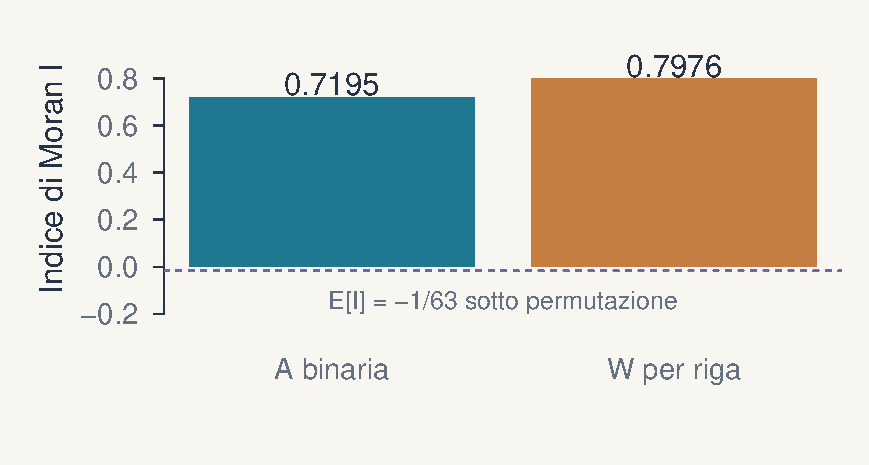
\includegraphics[width=9.85cm,height=5.25cm,keepaspectratio]{Risultati/Figure/18_Moran_confronto.pdf}
\vspace{1.5mm}
\PSmall{Confronto degli indici calcolati sugli stessi 64 siti con matrice binaria e normalizzazione di riga.}

\end{minipage}\end{lrbox}
\typeout{FULLBOX:059:PilotLeftBox:\the\ht\PilotLeftBox:\the\dp\PilotLeftBox}

\begin{lrbox}{\PilotRightBox}
\begin{minipage}[t]{7.55cm}\raggedright\color{Ink}\fontsize{11.3}{14.8}\selectfont
\PBody{Il calcolo restituisce $I_A=0,720$ e $I_W=0,798$. Entrambi sono positivi: tendono a essere collegati scarti dello stesso segno.}
\vspace{2.5mm}
\PInfo{La differenza fra i due indici non è un errore di calcolo. I siti con gradi diversi ricevono contributi differenti.}
\PBody{Per stabilire quanto un valore sia insolito, occorre confrontarlo con un riferimento costruito usando gli stessi pesi.}
\vspace{2.5mm}

\end{minipage}\end{lrbox}
\typeout{FULLBOX:059:PilotRightBox:\the\ht\PilotRightBox:\the\dp\PilotRightBox}

\begin{tikzpicture}[remember picture,overlay]
\PilotChrome{Pesi differenti producono indici differenti}{V · ASSOCIAZIONE SPAZIALE}{59}{Un indice di associazione è inseparabile dalla matrice con cui è stato calcolato.}
\node[anchor=north west,inner sep=0] at([xshift=.96cm,yshift=-2.13cm]current page.north west){\usebox{\PilotLeftBox}};
\node[anchor=north west,inner sep=0] at([xshift=11.52cm,yshift=-2.13cm]current page.north west){\usebox{\PilotRightBox}};
\node[anchor=north east,inner sep=0] at([xshift=17.65cm,yshift=-12.06cm]current page.north west){\color{Classical}\fontsize{7.7}{9.2}\selectfont\href{../../03_Notebook_svolti/M11_Locus/M11_N13.html}{M11\_N13 · notebook svolto}};
\end{tikzpicture}\end{frame}

\begin{frame}[plain]\hypertarget{slide60}{}
\bookmark[level=1,page=60]{Lo scatter di Moran usa il ritardo spaziale}
\begin{lrbox}{\TitleBox}
\begin{minipage}[t]{17.7cm}\raggedright\color{Ink}\fontsize{11.3}{14.8}\selectfont
\color{Navy}\bfseries\fontsize{20.6}{24.5}\selectfont Lo scatter di Moran usa il ritardo spaziale
\end{minipage}\end{lrbox}
\typeout{FULLBOX:060:TitleBox:\the\ht\TitleBox:\the\dp\TitleBox}

\begin{lrbox}{\RecallBox}
\begin{minipage}[t]{14.3cm}\raggedright\color{Ink}\fontsize{11.3}{14.8}\selectfont
\fontsize{10.3}{13.8}\selectfont La pendenza dello scatter coincide con l’indice basato sugli stessi pesi di riga.
\end{minipage}\end{lrbox}
\typeout{FULLBOX:060:RecallBox:\the\ht\RecallBox:\the\dp\RecallBox}

\begin{lrbox}{\PilotLeftBox}
\begin{minipage}[t]{10.05cm}\raggedright\color{Ink}\fontsize{11.3}{14.8}\selectfont
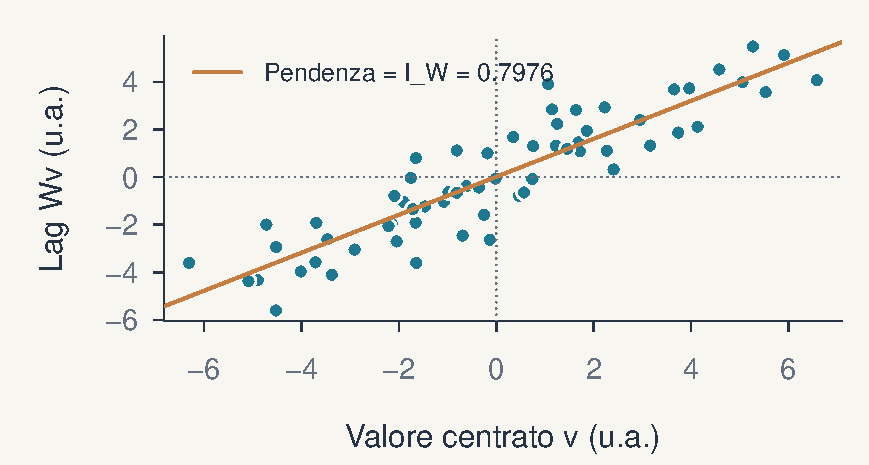
\includegraphics[width=9.85cm,height=5.25cm,keepaspectratio]{Risultati/Figure/19_Moran_scatter.pdf}
\vspace{1.5mm}
\PSmall{Ascissa: $v=z-\bar z$; ordinata: $Wv$. La pendenza della regressione con intercetta è $I_W$.}

\end{minipage}\end{lrbox}
\typeout{FULLBOX:060:PilotLeftBox:\the\ht\PilotLeftBox:\the\dp\PilotLeftBox}

\begin{lrbox}{\PilotRightBox}
\begin{minipage}[t]{7.55cm}\raggedright\color{Ink}\fontsize{11.3}{14.8}\selectfont
\PBody{Il grafico confronta lo scarto del sito con la media pesata degli scarti dei suoi vicini.}
\vspace{2.5mm}
\PInfo{Poiché la media di v è zero, la pendenza coincide con $v^\top Wv/v^\top v$. La media di $Wv$ può non essere zero: W non è necessariamente doppiamente stocastica.}
\PCode{R · verificare la pendenza}{060_esempio.R}
\end{minipage}\end{lrbox}
\typeout{FULLBOX:060:PilotRightBox:\the\ht\PilotRightBox:\the\dp\PilotRightBox}

\begin{tikzpicture}[remember picture,overlay]
\PilotChrome{Lo scatter di Moran usa il ritardo spaziale}{V · ASSOCIAZIONE SPAZIALE}{60}{La pendenza dello scatter coincide con l’indice basato sugli stessi pesi di riga.}
\node[anchor=north west,inner sep=0] at([xshift=.96cm,yshift=-2.13cm]current page.north west){\usebox{\PilotLeftBox}};
\node[anchor=north west,inner sep=0] at([xshift=11.52cm,yshift=-2.13cm]current page.north west){\usebox{\PilotRightBox}};
\node[anchor=north east,inner sep=0] at([xshift=17.65cm,yshift=-12.06cm]current page.north west){\color{Classical}\fontsize{7.7}{9.2}\selectfont\href{../../03_Notebook_svolti/M11_Locus/M11_N13.html}{M11\_N13 · notebook svolto}};
\end{tikzpicture}\end{frame}

\begin{frame}[plain]\hypertarget{slide61}{}
\bookmark[level=1,page=61]{I quadranti descrivono configurazioni locali}
\begin{lrbox}{\TitleBox}
\begin{minipage}[t]{17.7cm}\raggedright\color{Ink}\fontsize{11.3}{14.8}\selectfont
\color{Navy}\bfseries\fontsize{20.6}{24.5}\selectfont I quadranti descrivono configurazioni locali
\end{minipage}\end{lrbox}
\typeout{FULLBOX:061:TitleBox:\the\ht\TitleBox:\the\dp\TitleBox}

\begin{lrbox}{\RecallBox}
\begin{minipage}[t]{14.3cm}\raggedright\color{Ink}\fontsize{11.3}{14.8}\selectfont
\fontsize{10.3}{13.8}\selectfont Una classificazione descrittiva dei siti non equivale a una mappa di significatività.
\end{minipage}\end{lrbox}
\typeout{FULLBOX:061:RecallBox:\the\ht\RecallBox:\the\dp\RecallBox}

\begin{lrbox}{\PilotLeftBox}
\begin{minipage}[t]{10.05cm}\raggedright\color{Ink}\fontsize{11.3}{14.8}\selectfont
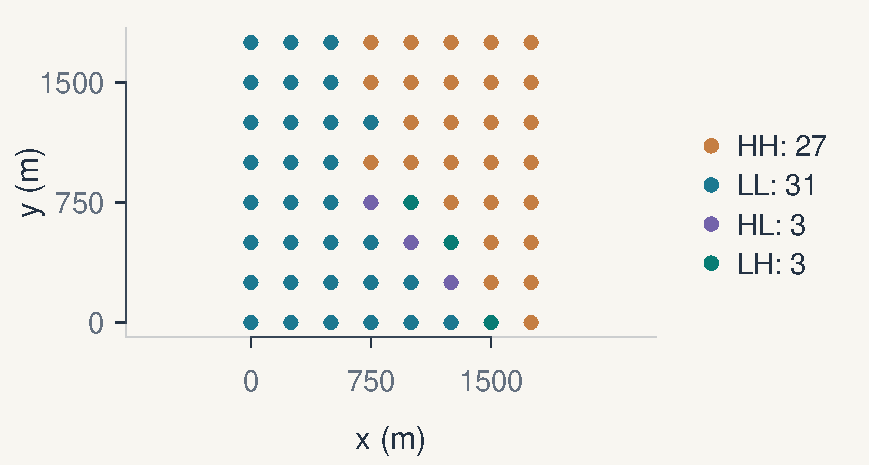
\includegraphics[width=9.85cm,height=5.25cm,keepaspectratio]{Risultati/Figure/20_quadranti.pdf}
\vspace{1.5mm}
\PSmall{La classificazione usa il segno dello scarto e del ritardo. È descrittiva.}

\end{minipage}\end{lrbox}
\typeout{FULLBOX:061:PilotLeftBox:\the\ht\PilotLeftBox:\the\dp\PilotLeftBox}

\begin{lrbox}{\PilotRightBox}
\begin{minipage}[t]{7.55cm}\raggedright\color{Ink}\fontsize{11.3}{14.8}\selectfont
\PBody{Due segni positivi descrivono un valore alto con vicini mediamente alti; due segni negativi indicano basso con basso. Segni opposti descrivono un contrasto fra sito e vicinato.}
\vspace{2.5mm}
\PInfo{Un quadrante non è un test locale. Per inferenze sito per sito servono una statistica locale, un riferimento appropriato e attenzione ai confronti multipli.}
\PBody{Alto e basso si riferiscono alla media globale. Non indicano soglie scientifiche esterne.}
\vspace{2.5mm}

\end{minipage}\end{lrbox}
\typeout{FULLBOX:061:PilotRightBox:\the\ht\PilotRightBox:\the\dp\PilotRightBox}

\begin{tikzpicture}[remember picture,overlay]
\PilotChrome{I quadranti descrivono configurazioni locali}{V · ASSOCIAZIONE SPAZIALE}{61}{Una classificazione descrittiva dei siti non equivale a una mappa di significatività.}
\node[anchor=north west,inner sep=0] at([xshift=.96cm,yshift=-2.13cm]current page.north west){\usebox{\PilotLeftBox}};
\node[anchor=north west,inner sep=0] at([xshift=11.52cm,yshift=-2.13cm]current page.north west){\usebox{\PilotRightBox}};
\end{tikzpicture}\end{frame}

\begin{frame}[plain]\hypertarget{slide62}{}
\bookmark[level=1,page=62]{Moran è invariante a traslazione e scala}
\begin{lrbox}{\TitleBox}
\begin{minipage}[t]{17.7cm}\raggedright\color{Ink}\fontsize{11.3}{14.8}\selectfont
\color{Navy}\bfseries\fontsize{20.6}{24.5}\selectfont Moran è invariante a traslazione e scala
\end{minipage}\end{lrbox}
\typeout{FULLBOX:062:TitleBox:\the\ht\TitleBox:\the\dp\TitleBox}

\begin{lrbox}{\RecallBox}
\begin{minipage}[t]{14.3cm}\raggedright\color{Ink}\fontsize{11.3}{14.8}\selectfont
\fontsize{10.3}{13.8}\selectfont L’invarianza di una statistica non si estende automaticamente a tutte le quantità dell’analisi.
\end{minipage}\end{lrbox}
\typeout{FULLBOX:062:RecallBox:\the\ht\RecallBox:\the\dp\RecallBox}

\begin{lrbox}{\PilotLeftBox}
\begin{minipage}[t]{10.05cm}\raggedright\color{Ink}\fontsize{11.3}{14.8}\selectfont
\[z^\star=a+bz,\qquad b\ne0\quad\Longrightarrow\quad I_H(z^\star)=I_H(z)\]
\PInfo{Gli scarti vengono moltiplicati per b. Numeratore e denominatore sono quindi moltiplicati per $b^2$.}

\end{minipage}\end{lrbox}
\typeout{FULLBOX:062:PilotLeftBox:\the\ht\PilotLeftBox:\the\dp\PilotLeftBox}

\begin{lrbox}{\PilotRightBox}
\begin{minipage}[t]{7.55cm}\raggedright\color{Ink}\fontsize{11.3}{14.8}\selectfont
\PBody{Cambiare l’unità con una trasformazione affine non cambia l’indice. Una trasformazione non lineare può invece modificarlo.}
\vspace{2.5mm}
\PBody{Questa proprietà non rende irrilevanti le unità per tutte le analisi: semivarianze, errori e soglie scientifiche mantengono unità proprie.}
\vspace{2.5mm}
\PCode{R · invarianza affine}{062_esempio.R}
\end{minipage}\end{lrbox}
\typeout{FULLBOX:062:PilotRightBox:\the\ht\PilotRightBox:\the\dp\PilotRightBox}

\begin{tikzpicture}[remember picture,overlay]
\PilotChrome{Moran è invariante a traslazione e scala}{V · ASSOCIAZIONE SPAZIALE}{62}{L’invarianza di una statistica non si estende automaticamente a tutte le quantità dell’analisi.}
\node[anchor=north west,inner sep=0] at([xshift=.96cm,yshift=-2.13cm]current page.north west){\usebox{\PilotLeftBox}};
\node[anchor=north west,inner sep=0] at([xshift=11.52cm,yshift=-2.13cm]current page.north west){\usebox{\PilotRightBox}};
\node[anchor=north east,inner sep=0] at([xshift=17.65cm,yshift=-12.06cm]current page.north west){\color{Classical}\fontsize{7.7}{9.2}\selectfont\href{../../03_Notebook_svolti/M11_Locus/M11_N13.html}{M11\_N13 · notebook svolto}};
\end{tikzpicture}\end{frame}

\begin{frame}[plain]\hypertarget{slide63}{}
\bookmark[level=1,page=63]{Permutare mantiene fissa la geometria}
\begin{lrbox}{\TitleBox}
\begin{minipage}[t]{17.7cm}\raggedright\color{Ink}\fontsize{11.3}{14.8}\selectfont
\color{Navy}\bfseries\fontsize{20.6}{24.5}\selectfont Permutare mantiene fissa la geometria
\end{minipage}\end{lrbox}
\typeout{FULLBOX:063:TitleBox:\the\ht\TitleBox:\the\dp\TitleBox}

\begin{lrbox}{\RecallBox}
\begin{minipage}[t]{14.3cm}\raggedright\color{Ink}\fontsize{11.3}{14.8}\selectfont
\fontsize{10.3}{13.8}\selectfont Nel test per permutazione restano fissi valori disponibili, siti e pesi; cambia la loro associazione.
\end{minipage}\end{lrbox}
\typeout{FULLBOX:063:RecallBox:\the\ht\RecallBox:\the\dp\RecallBox}

\begin{lrbox}{\PilotLeftBox}
\begin{minipage}[t]{10.05cm}\raggedright\color{Ink}\fontsize{11.3}{14.8}\selectfont
\begin{tikzpicture}[x=1cm,y=1cm]
\path[use as bounding box](-.1,-.15) rectangle(9.7,4.8);
\node[pFlow,text width=3.7cm,fill=GeoA!7] (a) at(2.2,3.8){Coordinate e pesi restano fissi};
\node[pFlow,text width=3.7cm,fill=GeoB!7] (b) at(7.2,3.8){Valori osservati vengono permutati};
\node[pFlow,text width=3.7cm,fill=GeoA!7] (c) at(2.2,1.15){Statistica osservata\\$I_{\mathrm{obs}}$};
\node[pFlow,text width=3.7cm,fill=GeoC!7] (d) at(7.2,1.15){Riferimento nullo\\$I^{(1)},\ldots,I^{(B)}$};
\draw[pEdge] (a) -- (c);
\draw[pEdge] (b) -- (d);
\draw[pEdge] (c) -- node[pNote,fill=Paper,inner sep=1pt]{rango} (d);
\end{tikzpicture}

\end{minipage}\end{lrbox}
\typeout{FULLBOX:063:PilotLeftBox:\the\ht\PilotLeftBox:\the\dp\PilotLeftBox}

\begin{lrbox}{\PilotRightBox}
\begin{minipage}[t]{7.55cm}\raggedright\color{Ink}\fontsize{11.3}{14.8}\selectfont
\PBody{Il riferimento riassegna gli stessi valori ai siti, mantenendo coordinate e matrice dei pesi. Ogni permutazione produce un nuovo indice.}
\vspace{2.5mm}
\PInfo{La domanda è se l’associazione osservata sia insolita rispetto alla riassegnazione dei valori ammessa dall’ipotesi nulla.}
\PBody{La permutazione non simula nuovi campioni geologici: costruisce un riferimento condizionato ai valori osservati.}
\vspace{2.5mm}

\end{minipage}\end{lrbox}
\typeout{FULLBOX:063:PilotRightBox:\the\ht\PilotRightBox:\the\dp\PilotRightBox}

\begin{tikzpicture}[remember picture,overlay]
\PilotChrome{Permutare mantiene fissa la geometria}{V · ASSOCIAZIONE SPAZIALE}{63}{Nel test per permutazione restano fissi valori disponibili, siti e pesi; cambia la loro associazione.}
\node[anchor=north west,inner sep=0] at([xshift=.96cm,yshift=-2.13cm]current page.north west){\usebox{\PilotLeftBox}};
\node[anchor=north west,inner sep=0] at([xshift=11.52cm,yshift=-2.13cm]current page.north west){\usebox{\PilotRightBox}};
\node[anchor=north east,inner sep=0] at([xshift=17.65cm,yshift=-12.06cm]current page.north west){\color{Classical}\fontsize{7.7}{9.2}\selectfont\href{../../03_Notebook_svolti/M11_Locus/M11_N14.html}{M11\_N14 · notebook svolto}};
\end{tikzpicture}\end{frame}

\begin{frame}[plain]\hypertarget{slide64}{}
\bookmark[level=1,page=64]{L’ipotesi nulla richiede scambiabilità}
\begin{lrbox}{\TitleBox}
\begin{minipage}[t]{17.7cm}\raggedright\color{Ink}\fontsize{11.3}{14.8}\selectfont
\color{Navy}\bfseries\fontsize{20.6}{24.5}\selectfont L’ipotesi nulla richiede scambiabilità
\end{minipage}\end{lrbox}
\typeout{FULLBOX:064:TitleBox:\the\ht\TitleBox:\the\dp\TitleBox}

\begin{lrbox}{\RecallBox}
\begin{minipage}[t]{14.3cm}\raggedright\color{Ink}\fontsize{11.3}{14.8}\selectfont
\fontsize{10.3}{13.8}\selectfont Il significato del test dipende da quali riassegnazioni sono giustificate dall’ipotesi nulla.
\end{minipage}\end{lrbox}
\typeout{FULLBOX:064:RecallBox:\the\ht\RecallBox:\the\dp\RecallBox}

\begin{lrbox}{\PilotLeftBox}
\begin{minipage}[t]{10.05cm}\raggedright\color{Ink}\fontsize{11.3}{14.8}\selectfont
\[H_0:\ (Z(s_1),\ldots,Z(s_n))\ \text{è scambiabile rispetto ai siti}\]
\[\mathbb E_{\mathrm{perm}}(I_H)=-\frac{1}{n-1}\quad\text{con diagonale nulla}\]
\PInfo{Il valore atteso riguarda la permutazione completa delle etichette, per valori non costanti e pesi fissati. Non è una descrizione universale di ogni processo spaziale.}

\end{minipage}\end{lrbox}
\typeout{FULLBOX:064:PilotLeftBox:\the\ht\PilotLeftBox:\the\dp\PilotLeftBox}

\begin{lrbox}{\PilotRightBox}
\begin{minipage}[t]{7.55cm}\raggedright\color{Ink}\fontsize{11.3}{14.8}\selectfont
\PBody{Un trend legato alla posizione rende i valori di luoghi diversi non equivalenti. La riassegnazione libera rompe anche quel trend.}
\vspace{2.5mm}
\PBody{Un rifiuto dell’ipotesi nulla non separa automaticamente gradiente, dipendenza residua e altre cause della disposizione osservata.}
\vspace{2.5mm}

\end{minipage}\end{lrbox}
\typeout{FULLBOX:064:PilotRightBox:\the\ht\PilotRightBox:\the\dp\PilotRightBox}

\begin{tikzpicture}[remember picture,overlay]
\PilotChrome{L’ipotesi nulla richiede scambiabilità}{V · ASSOCIAZIONE SPAZIALE}{64}{Il significato del test dipende da quali riassegnazioni sono giustificate dall’ipotesi nulla.}
\node[anchor=north west,inner sep=0] at([xshift=.96cm,yshift=-2.13cm]current page.north west){\usebox{\PilotLeftBox}};
\node[anchor=north west,inner sep=0] at([xshift=11.52cm,yshift=-2.13cm]current page.north west){\usebox{\PilotRightBox}};
\node[anchor=north east,inner sep=0] at([xshift=17.65cm,yshift=-12.06cm]current page.north west){\color{Classical}\fontsize{7.7}{9.2}\selectfont\href{../../03_Notebook_svolti/M11_Locus/M11_N14.html}{M11\_N14 · notebook svolto}};
\end{tikzpicture}\end{frame}

\begin{frame}[plain]\hypertarget{slide65}{}
\bookmark[level=1,page=65]{Il p-value Monte Carlo include il caso osservato}
\begin{lrbox}{\TitleBox}
\begin{minipage}[t]{17.7cm}\raggedright\color{Ink}\fontsize{11.3}{14.8}\selectfont
\color{Navy}\bfseries\fontsize{20.6}{24.5}\selectfont Il p-value Monte Carlo include il caso osservato
\end{minipage}\end{lrbox}
\typeout{FULLBOX:065:TitleBox:\the\ht\TitleBox:\the\dp\TitleBox}

\begin{lrbox}{\RecallBox}
\begin{minipage}[t]{14.3cm}\raggedright\color{Ink}\fontsize{11.3}{14.8}\selectfont
\fontsize{10.3}{13.8}\selectfont Il p-value misura compatibilità con un riferimento esplicito e ha una risoluzione finita.
\end{minipage}\end{lrbox}
\typeout{FULLBOX:065:RecallBox:\the\ht\RecallBox:\the\dp\RecallBox}

\begin{lrbox}{\PilotLeftBox}
\begin{minipage}[t]{10.05cm}\raggedright\color{Ink}\fontsize{11.3}{14.8}\selectfont
\[p_{\mathrm{MC}}=\frac{1+\sum_{b=1}^{B}\mathbf1(I^{(b)}\ge I_{\mathrm{obs}})}{B+1}\]
\PInfo{Usiamo l’alternativa unilaterale di associazione positiva. La direzione viene dichiarata prima di leggere il risultato.}

\end{minipage}\end{lrbox}
\typeout{FULLBOX:065:PilotLeftBox:\the\ht\PilotLeftBox:\the\dp\PilotLeftBox}

\begin{lrbox}{\PilotRightBox}
\begin{minipage}[t]{7.55cm}\raggedright\color{Ink}\fontsize{11.3}{14.8}\selectfont
\PBody{Il numeratore conta le permutazioni almeno tanto estreme quanto l’osservazione, più il caso osservato. Il p-value non è mai zero.}
\vspace{2.5mm}
\PBody{Le 100 permutazioni originali usano blocchi di uniformi salvati nel CSV.}
\vspace{2.5mm}
\PCode{R · riferimento originale N14}{065_esempio.R}
\end{minipage}\end{lrbox}
\typeout{FULLBOX:065:PilotRightBox:\the\ht\PilotRightBox:\the\dp\PilotRightBox}

\begin{tikzpicture}[remember picture,overlay]
\PilotChrome{Il p-value Monte Carlo include il caso osservato}{V · ASSOCIAZIONE SPAZIALE}{65}{Il p-value misura compatibilità con un riferimento esplicito e ha una risoluzione finita.}
\node[anchor=north west,inner sep=0] at([xshift=.96cm,yshift=-2.13cm]current page.north west){\usebox{\PilotLeftBox}};
\node[anchor=north west,inner sep=0] at([xshift=11.52cm,yshift=-2.13cm]current page.north west){\usebox{\PilotRightBox}};
\node[anchor=north east,inner sep=0] at([xshift=17.65cm,yshift=-12.06cm]current page.north west){\color{Classical}\fontsize{7.7}{9.2}\selectfont\href{../../03_Notebook_svolti/M11_Locus/M11_N14.html}{M11\_N14 · notebook svolto}};
\end{tikzpicture}\end{frame}

\begin{frame}[plain]\hypertarget{slide66}{}
\bookmark[level=1,page=66]{Il numero di permutazioni limita la risoluzione}
\begin{lrbox}{\TitleBox}
\begin{minipage}[t]{17.7cm}\raggedright\color{Ink}\fontsize{11.3}{14.8}\selectfont
\color{Navy}\bfseries\fontsize{20.6}{24.5}\selectfont Il numero di permutazioni limita la risoluzione
\end{minipage}\end{lrbox}
\typeout{FULLBOX:066:TitleBox:\the\ht\TitleBox:\the\dp\TitleBox}

\begin{lrbox}{\RecallBox}
\begin{minipage}[t]{14.3cm}\raggedright\color{Ink}\fontsize{11.3}{14.8}\selectfont
\fontsize{10.3}{13.8}\selectfont La precisione Monte Carlo e l’adeguatezza del riferimento inferenziale sono proprietà distinte.
\end{minipage}\end{lrbox}
\typeout{FULLBOX:066:RecallBox:\the\ht\RecallBox:\the\dp\RecallBox}

\begin{lrbox}{\PilotLeftBox}
\begin{minipage}[t]{10.05cm}\raggedright\color{Ink}\fontsize{11.3}{14.8}\selectfont
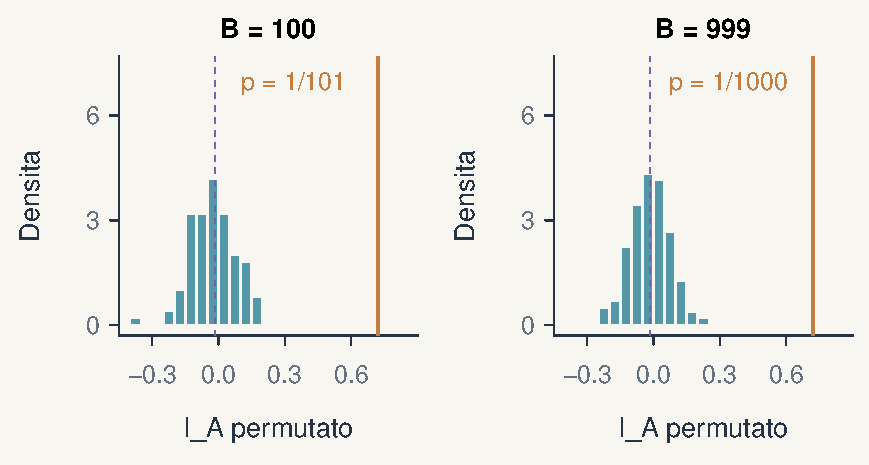
\includegraphics[width=9.85cm,height=5.25cm,keepaspectratio]{Risultati/Figure/21_permutazioni100_999.pdf}
\vspace{1.5mm}
\PSmall{Protocollo originale con B=100 e approfondimento con B=999. Pesi e alternativa restano dichiarati.}

\end{minipage}\end{lrbox}
\typeout{FULLBOX:066:PilotLeftBox:\the\ht\PilotLeftBox:\the\dp\PilotLeftBox}

\begin{lrbox}{\PilotRightBox}
\begin{minipage}[t]{7.55cm}\raggedright\color{Ink}\fontsize{11.3}{14.8}\selectfont
\PBody{Con 100 permutazioni la risoluzione minima è $1/101$. Con 999 diventa $1/1000$. Aumentare B rende più fine la stima Monte Carlo.}
\vspace{2.5mm}
\PInfo{Più permutazioni non correggono un’ipotesi di scambiabilità sbagliata. Il seme riproduce l’estrazione, ma non garantisce la validità dell’inferenza.}
\PCode{R · approfondimento dichiarato}{066_esempio.R}
\end{minipage}\end{lrbox}
\typeout{FULLBOX:066:PilotRightBox:\the\ht\PilotRightBox:\the\dp\PilotRightBox}

\begin{tikzpicture}[remember picture,overlay]
\PilotChrome{Il numero di permutazioni limita la risoluzione}{V · ASSOCIAZIONE SPAZIALE}{66}{La precisione Monte Carlo e l’adeguatezza del riferimento inferenziale sono proprietà distinte.}
\node[anchor=north west,inner sep=0] at([xshift=.96cm,yshift=-2.13cm]current page.north west){\usebox{\PilotLeftBox}};
\node[anchor=north west,inner sep=0] at([xshift=11.52cm,yshift=-2.13cm]current page.north west){\usebox{\PilotRightBox}};
\node[anchor=north east,inner sep=0] at([xshift=17.65cm,yshift=-12.06cm]current page.north west){\color{Classical}\fontsize{7.7}{9.2}\selectfont\href{../../03_Notebook_svolti/M11_Locus/M11_N14.html}{M11\_N14 · notebook svolto}};
\end{tikzpicture}\end{frame}

\begin{frame}[plain]\hypertarget{slide67}{}
\bookmark[level=1,page=67]{Un gradiente può generare associazione globale}
\begin{lrbox}{\TitleBox}
\begin{minipage}[t]{17.7cm}\raggedright\color{Ink}\fontsize{11.3}{14.8}\selectfont
\color{Navy}\bfseries\fontsize{20.6}{24.5}\selectfont Un gradiente può generare associazione globale
\end{minipage}\end{lrbox}
\typeout{FULLBOX:067:TitleBox:\the\ht\TitleBox:\the\dp\TitleBox}

\begin{lrbox}{\RecallBox}
\begin{minipage}[t]{14.3cm}\raggedright\color{Ink}\fontsize{11.3}{14.8}\selectfont
\fontsize{10.3}{13.8}\selectfont L’associazione globale non distingue da sola un trend da una dipendenza residua.
\end{minipage}\end{lrbox}
\typeout{FULLBOX:067:RecallBox:\the\ht\RecallBox:\the\dp\RecallBox}

\begin{lrbox}{\FullWideBox}
\begin{minipage}[t]{18.1cm}\raggedright\color{Ink}\fontsize{11.3}{14.8}\selectfont
\centering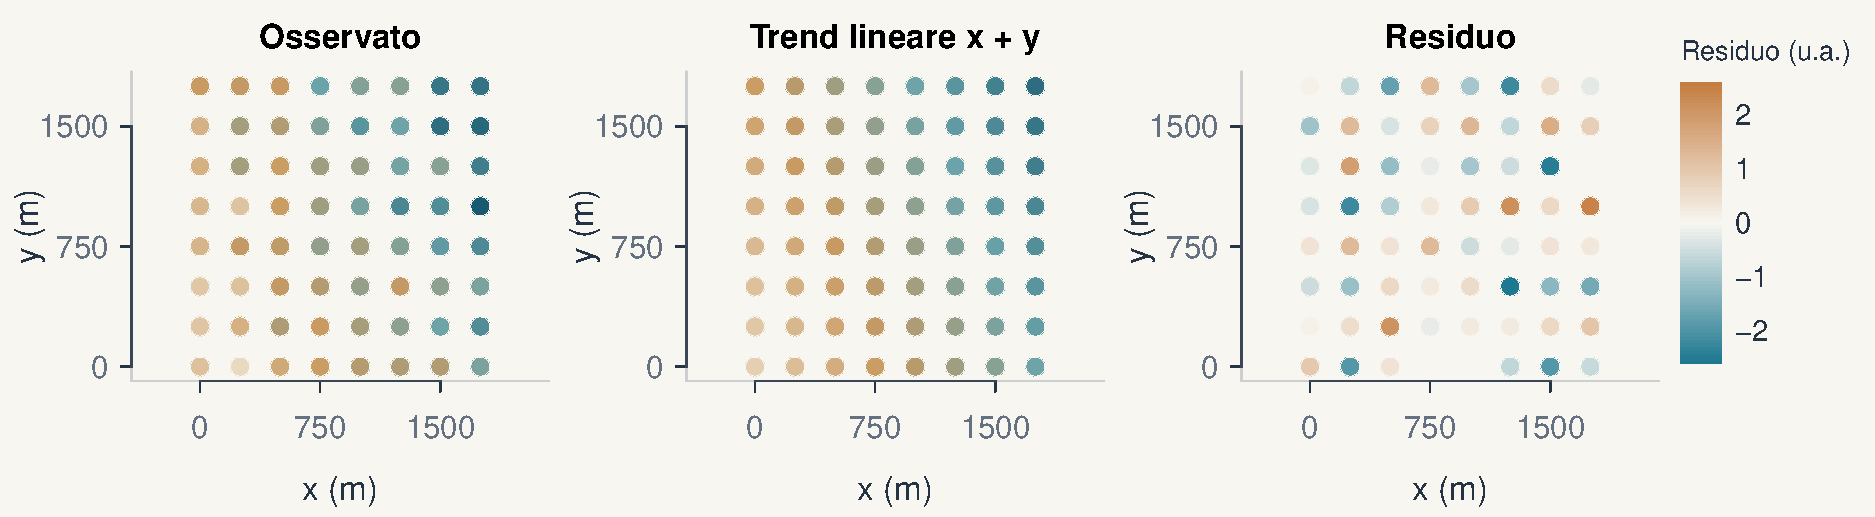
\includegraphics[width=18.05cm,height=5.8cm,keepaspectratio]{Risultati/Figure/22_trend_residui.pdf}
\end{minipage}\end{lrbox}
\typeout{FULLBOX:067:FullWideBox:\the\ht\FullWideBox:\the\dp\FullWideBox}

\begin{lrbox}{\PilotRightBox}
\begin{minipage}[t]{18.1cm}\raggedright\color{Ink}\fontsize{11.3}{14.8}\selectfont
\PBody{Sui dati $I_A=0,720$; sui residui del piano $I_A=-0,040$. Il confronto è descrittivo: parte dell’associazione globale è legata alla variazione della media. La domanda sulla dipendenza residua richiede un riferimento coerente con la stima del piano. Non si presenta una permutazione libera dei residui come test esatto.}
\end{minipage}\end{lrbox}
\typeout{FULLBOX:067:PilotRightBox:\the\ht\PilotRightBox:\the\dp\PilotRightBox}

\begin{tikzpicture}[remember picture,overlay]
\PilotChrome{Un gradiente può generare associazione globale}{V · ASSOCIAZIONE SPAZIALE}{67}{L’associazione globale non distingue da sola un trend da una dipendenza residua.}
\node[anchor=north west,inner sep=0] at([xshift=.96cm,yshift=-2.13cm]current page.north west){\usebox{\FullWideBox}};
\node[anchor=north west,inner sep=0] at([xshift=.96cm,yshift=-8.25cm]current page.north west){\usebox{\PilotRightBox}};
\end{tikzpicture}\end{frame}

\begin{frame}[plain]\hypertarget{slide68}{}
\bookmark[level=1,page=68]{I residui sono stimati e hanno vincoli}
\begin{lrbox}{\TitleBox}
\begin{minipage}[t]{17.7cm}\raggedright\color{Ink}\fontsize{11.3}{14.8}\selectfont
\color{Navy}\bfseries\fontsize{20.6}{24.5}\selectfont I residui sono stimati e hanno vincoli
\end{minipage}\end{lrbox}
\typeout{FULLBOX:068:TitleBox:\the\ht\TitleBox:\the\dp\TitleBox}

\begin{lrbox}{\RecallBox}
\begin{minipage}[t]{14.3cm}\raggedright\color{Ink}\fontsize{11.3}{14.8}\selectfont
\fontsize{10.3}{13.8}\selectfont La stima della tendenza modifica la struttura probabilistica dei residui.
\end{minipage}\end{lrbox}
\typeout{FULLBOX:068:RecallBox:\the\ht\RecallBox:\the\dp\RecallBox}

\begin{lrbox}{\PilotLeftBox}
\begin{minipage}[t]{10.05cm}\raggedright\color{Ink}\fontsize{11.3}{14.8}\selectfont
\[Z(s)=m(s)+\varepsilon(s),\qquad \widehat e_i=z_i-\widehat m(s_i)\]
\[\widehat{\boldsymbol e}=(I-H)\boldsymbol z\]
\PInfo{Anche con errori indipendenti omoschedastici, i residui OLS hanno covarianza proporzionale a $I-H$. Non sono automaticamente scambiabili.}

\end{minipage}\end{lrbox}
\typeout{FULLBOX:068:PilotLeftBox:\the\ht\PilotLeftBox:\the\dp\PilotLeftBox}

\begin{lrbox}{\PilotRightBox}
\begin{minipage}[t]{7.55cm}\raggedright\color{Ink}\fontsize{11.3}{14.8}\selectfont
\PBody{Il confronto degli indici sui dati e sui residui è descrittivo. Una permutazione libera dei residui non fornisce in generale un test esatto.}
\vspace{2.5mm}
\PBody{Per l’inferenza occorre un metodo giustificato dal modello: per esempio una simulazione coerente con l’ipotesi nulla e con la stima.}
\vspace{2.5mm}
\PCode{R · diagnosi descrittiva}{068_esempio.R}
\end{minipage}\end{lrbox}
\typeout{FULLBOX:068:PilotRightBox:\the\ht\PilotRightBox:\the\dp\PilotRightBox}

\begin{tikzpicture}[remember picture,overlay]
\PilotChrome{I residui sono stimati e hanno vincoli}{V · ASSOCIAZIONE SPAZIALE}{68}{La stima della tendenza modifica la struttura probabilistica dei residui.}
\node[anchor=north west,inner sep=0] at([xshift=.96cm,yshift=-2.13cm]current page.north west){\usebox{\PilotLeftBox}};
\node[anchor=north west,inner sep=0] at([xshift=11.52cm,yshift=-2.13cm]current page.north west){\usebox{\PilotRightBox}};
\end{tikzpicture}\end{frame}

\begin{frame}[plain]\hypertarget{slide69}{}
\bookmark[level=1,page=69]{Associazione, significatività e meccanismo}
\begin{lrbox}{\TitleBox}
\begin{minipage}[t]{17.7cm}\raggedright\color{Ink}\fontsize{11.3}{14.8}\selectfont
\color{Navy}\bfseries\fontsize{20.6}{24.5}\selectfont Associazione, significatività e meccanismo
\end{minipage}\end{lrbox}
\typeout{FULLBOX:069:TitleBox:\the\ht\TitleBox:\the\dp\TitleBox}

\begin{lrbox}{\RecallBox}
\begin{minipage}[t]{14.3cm}\raggedright\color{Ink}\fontsize{11.3}{14.8}\selectfont
\fontsize{10.3}{13.8}\selectfont Una conclusione deve restare proporzionata alla domanda e al riferimento che sono stati verificati.
\end{minipage}\end{lrbox}
\typeout{FULLBOX:069:RecallBox:\the\ht\RecallBox:\the\dp\RecallBox}

\begin{lrbox}{\PilotLeftBox}
\begin{minipage}[t]{10.05cm}\raggedright\color{Ink}\fontsize{11.3}{14.8}\selectfont
{\fontsize{10.2}{13.1}\selectfont\renewcommand{\arraystretch}{1.45}\begin{tabular}{@{}p{4.2cm}p{4.8cm}@{}}\toprule
\textbf{Risultato} & \textbf{Che cosa consente di dire}\\\midrule
Indice positivo & Scarti simili contribuiscono sul grafo\\
p-value piccolo & Risultato insolito sotto il riferimento scelto\\
Mappa dei quadranti & Descrizione delle configurazioni\\
Spiegazione causale & Richiede disegno ed evidenze ulteriori\\
\bottomrule\end{tabular}}

\end{minipage}\end{lrbox}
\typeout{FULLBOX:069:PilotLeftBox:\the\ht\PilotLeftBox:\the\dp\PilotLeftBox}

\begin{lrbox}{\PilotRightBox}
\begin{minipage}[t]{7.55cm}\raggedright\color{Ink}\fontsize{11.3}{14.8}\selectfont
\PBody{Un indice globale non identifica un processo di trasporto, una sorgente o una causa. La geometria può essere compatibile con meccanismi diversi.}
\vspace{2.5mm}
\PInfo{Nel dataset sintetico conosciamo il contesto didattico. La discussione serve a distinguere ciò che la statistica misura da ciò che una ricerca reale dovrebbe dimostrare.}
\PBody{Riportiamo insieme grandezza dell’indice, pesi, ipotesi nulla e limite interpretativo.}
\vspace{2.5mm}

\end{minipage}\end{lrbox}
\typeout{FULLBOX:069:PilotRightBox:\the\ht\PilotRightBox:\the\dp\PilotRightBox}

\begin{tikzpicture}[remember picture,overlay]
\PilotChrome{Associazione, significatività e meccanismo}{V · ASSOCIAZIONE SPAZIALE}{69}{Una conclusione deve restare proporzionata alla domanda e al riferimento che sono stati verificati.}
\node[anchor=north west,inner sep=0] at([xshift=.96cm,yshift=-2.13cm]current page.north west){\usebox{\PilotLeftBox}};
\node[anchor=north west,inner sep=0] at([xshift=11.52cm,yshift=-2.13cm]current page.north west){\usebox{\PilotRightBox}};
\end{tikzpicture}\end{frame}

\begin{frame}[plain]\hypertarget{slide70}{}
\bookmark[level=1,page=70]{Laboratorio: una frase completa su Moran}
\begin{lrbox}{\TitleBox}
\begin{minipage}[t]{17.7cm}\raggedright\color{Ink}\fontsize{11.3}{14.8}\selectfont
\color{Navy}\bfseries\fontsize{20.6}{24.5}\selectfont Laboratorio: una frase completa su Moran
\end{minipage}\end{lrbox}
\typeout{FULLBOX:070:TitleBox:\the\ht\TitleBox:\the\dp\TitleBox}

\begin{lrbox}{\RecallBox}
\begin{minipage}[t]{14.3cm}\raggedright\color{Ink}\fontsize{11.3}{14.8}\selectfont
\fontsize{10.3}{13.8}\selectfont Un risultato inferenziale leggibile include dati, pesi, ipotesi, alternativa e limiti.
\end{minipage}\end{lrbox}
\typeout{FULLBOX:070:RecallBox:\the\ht\RecallBox:\the\dp\RecallBox}

\begin{lrbox}{\PilotLeftBox}
\begin{minipage}[t]{10.05cm}\raggedright\color{Ink}\fontsize{11.3}{14.8}\selectfont
\PLab{https://marzione00.github.io/Lab_Geo/\#laboratorio/m11-moran}{Esperimento online · associazione e permutazioni}
{\fontsize{10.2}{13.1}\selectfont\renewcommand{\arraystretch}{1.45}\begin{tabular}{@{}p{3.1cm}p{5.9cm}@{}}\toprule
\textbf{Elemento della conclusione} & \textbf{Specificazione}\\\midrule
Dati & 64 concentrazioni sintetiche\\
Geometria & Piano locale, soglia 260 m\\
Pesi & Binari A per il risultato principale\\
Riferimento & Permutazione libera delle etichette\\
Alternativa & Associazione positiva\\
Limite & Trend e dipendenza residua non separati\\
\bottomrule\end{tabular}}

\end{minipage}\end{lrbox}
\typeout{FULLBOX:070:PilotLeftBox:\the\ht\PilotLeftBox:\the\dp\PilotLeftBox}

\begin{lrbox}{\PilotRightBox}
\begin{minipage}[t]{7.55cm}\raggedright\color{Ink}\fontsize{11.3}{14.8}\selectfont
\PBody{N13 calcola e verifica l’indice. N14 costruisce il riferimento e conserva il numero di permutazioni.}
\vspace{2.5mm}
\PInfo{Lo scatter usa W e la sua pendenza corrisponde a $I_W$. Questa specificazione deve comparire nella didascalia.}
\PBody{Il passo successivo studia come la dissimilarità cambi con la distanza.}
\vspace{2.5mm}

\end{minipage}\end{lrbox}
\typeout{FULLBOX:070:PilotRightBox:\the\ht\PilotRightBox:\the\dp\PilotRightBox}

\begin{tikzpicture}[remember picture,overlay]
\PilotChrome{Laboratorio: una frase completa su Moran}{V · ASSOCIAZIONE SPAZIALE}{70}{Un risultato inferenziale leggibile include dati, pesi, ipotesi, alternativa e limiti.}
\node[anchor=north west,inner sep=0] at([xshift=.96cm,yshift=-2.13cm]current page.north west){\usebox{\PilotLeftBox}};
\node[anchor=north west,inner sep=0] at([xshift=11.52cm,yshift=-2.13cm]current page.north west){\usebox{\PilotRightBox}};
\node[anchor=north east,inner sep=0] at([xshift=17.65cm,yshift=-12.06cm]current page.north west){\color{Classical}\fontsize{7.7}{9.2}\selectfont\href{../../03_Notebook_svolti/M11_Locus/M11_N14.html}{M11\_N14 · notebook svolto}};
\end{tikzpicture}\end{frame}

\begin{frame}[plain]\hypertarget{slide71}{}
\bookmark[level=0,page=71]{VI · SEMIVARIANZA}
\bookmark[level=1,page=71]{La semivarianza parte dalle coppie}
\begin{lrbox}{\TitleBox}
\begin{minipage}[t]{17.7cm}\raggedright\color{Ink}\fontsize{11.3}{14.8}\selectfont
\color{Navy}\bfseries\fontsize{20.6}{24.5}\selectfont La semivarianza parte dalle coppie
\end{minipage}\end{lrbox}
\typeout{FULLBOX:071:TitleBox:\the\ht\TitleBox:\the\dp\TitleBox}

\begin{lrbox}{\RecallBox}
\begin{minipage}[t]{14.3cm}\raggedright\color{Ink}\fontsize{11.3}{14.8}\selectfont
\fontsize{10.3}{13.8}\selectfont Le coppie descrivono dissimilarità a diverse separazioni, ma riutilizzano gli stessi siti.
\end{minipage}\end{lrbox}
\typeout{FULLBOX:071:RecallBox:\the\ht\RecallBox:\the\dp\RecallBox}

\begin{lrbox}{\PilotLeftBox}
\begin{minipage}[t]{10.05cm}\raggedright\color{Ink}\fontsize{11.3}{14.8}\selectfont
\begin{tikzpicture}[x=1cm,y=1cm]
\path[use as bounding box](-.1,-.15) rectangle(9.7,5.1);
\fill[GeoA](1.2,1.2)circle(4pt);
\fill[GeoB](7.9,3.8)circle(4pt);
\draw[GeoC,line width=1.2pt](1.2,1.2)--node[above,sloped,pLabel]{$h_{ij}=\|s_i-s_j\|$}(7.9,3.8);
\node[pLabel]at(1.3,.55){$z_i$};
\node[pLabel]at(7.9,4.4){$z_j$};
\node[pLabel]at(5.0,.8){contributo: $\tfrac12(z_i-z_j)^2$};
\end{tikzpicture}
\[g_{ij}=\tfrac12(z_i-z_j)^2,\qquad i<j\]

\end{minipage}\end{lrbox}
\typeout{FULLBOX:071:PilotLeftBox:\the\ht\PilotLeftBox:\the\dp\PilotLeftBox}

\begin{lrbox}{\PilotRightBox}
\begin{minipage}[t]{7.55cm}\raggedright\color{Ink}\fontsize{11.3}{14.8}\selectfont
\PBody{Per ogni coppia distinta calcoliamo distanza e metà del quadrato della differenza dei valori. Il contributo aumenta quando i campioni sono dissimili.}
\vspace{2.5mm}
\PInfo{Con 64 siti ci sono $64\cdot63/2=2016$ coppie non ordinate. La diagonale e le coppie replicate in ordine inverso vengono escluse.}
\PBody{La semivarianza ha unità pari al quadrato dell’unità della variabile: qui $(\mathrm{u.a.})^2$.}
\vspace{2.5mm}

\end{minipage}\end{lrbox}
\typeout{FULLBOX:071:PilotRightBox:\the\ht\PilotRightBox:\the\dp\PilotRightBox}

\begin{tikzpicture}[remember picture,overlay]
\PilotChrome{La semivarianza parte dalle coppie}{VI · SEMIVARIANZA}{71}{Le coppie descrivono dissimilarità a diverse separazioni, ma riutilizzano gli stessi siti.}
\node[anchor=north west,inner sep=0] at([xshift=.96cm,yshift=-2.13cm]current page.north west){\usebox{\PilotLeftBox}};
\node[anchor=north west,inner sep=0] at([xshift=11.52cm,yshift=-2.13cm]current page.north west){\usebox{\PilotRightBox}};
\node[anchor=north east,inner sep=0] at([xshift=17.65cm,yshift=-12.06cm]current page.north west){\color{Classical}\fontsize{7.7}{9.2}\selectfont\href{../../03_Notebook_svolti/M11_Locus/M11_N15.html}{M11\_N15 · notebook svolto}};
\end{tikzpicture}\end{frame}

\begin{frame}[plain]\hypertarget{slide72}{}
\bookmark[level=1,page=72]{La nube delle coppie precede la media per classe}
\begin{lrbox}{\TitleBox}
\begin{minipage}[t]{17.7cm}\raggedright\color{Ink}\fontsize{11.3}{14.8}\selectfont
\color{Navy}\bfseries\fontsize{20.6}{24.5}\selectfont La nube delle coppie precede la media per classe
\end{minipage}\end{lrbox}
\typeout{FULLBOX:072:TitleBox:\the\ht\TitleBox:\the\dp\TitleBox}

\begin{lrbox}{\RecallBox}
\begin{minipage}[t]{14.3cm}\raggedright\color{Ink}\fontsize{11.3}{14.8}\selectfont
\fontsize{10.3}{13.8}\selectfont Una curva media può nascondere una nube di coppie molto eterogenea.
\end{minipage}\end{lrbox}
\typeout{FULLBOX:072:RecallBox:\the\ht\RecallBox:\the\dp\RecallBox}

\begin{lrbox}{\PilotLeftBox}
\begin{minipage}[t]{10.05cm}\raggedright\color{Ink}\fontsize{11.3}{14.8}\selectfont
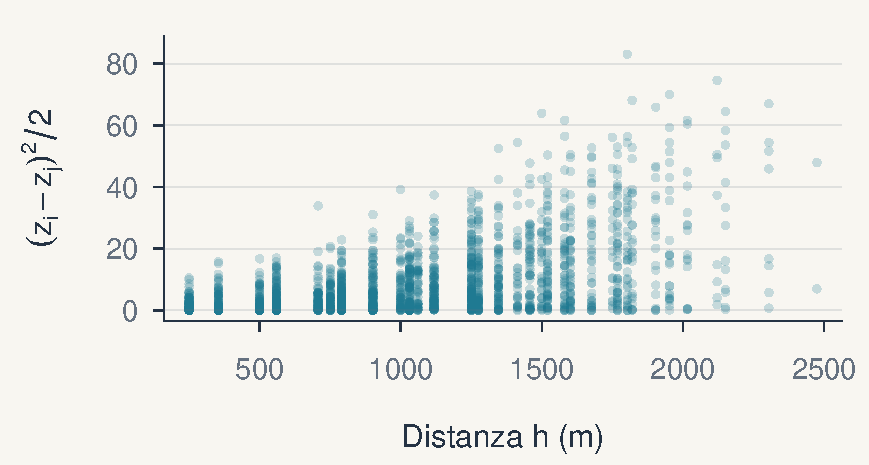
\includegraphics[width=9.85cm,height=5.25cm,keepaspectratio]{Risultati/Figure/23_coppie_semivarianza.pdf}
\vspace{1.5mm}
\PSmall{Ogni punto rappresenta una coppia: distanza in ascissa e semidifferenza quadratica in ordinata.}

\end{minipage}\end{lrbox}
\typeout{FULLBOX:072:PilotLeftBox:\the\ht\PilotLeftBox:\the\dp\PilotLeftBox}

\begin{lrbox}{\PilotRightBox}
\begin{minipage}[t]{7.55cm}\raggedright\color{Ink}\fontsize{11.3}{14.8}\selectfont
\PBody{Alla stessa distanza i contributi possono variare molto. La nube mostra dispersione e coppie influenti; le direzioni saranno analizzate a parte.}
\vspace{2.5mm}
\PInfo{Raggruppare le distanze riassume questa variabilità. Il riassunto non sostituisce l’ispezione dei dati da cui deriva.}
\PCode{R · coppie non ordinate}{072_esempio.R}
\end{minipage}\end{lrbox}
\typeout{FULLBOX:072:PilotRightBox:\the\ht\PilotRightBox:\the\dp\PilotRightBox}

\begin{tikzpicture}[remember picture,overlay]
\PilotChrome{La nube delle coppie precede la media per classe}{VI · SEMIVARIANZA}{72}{Una curva media può nascondere una nube di coppie molto eterogenea.}
\node[anchor=north west,inner sep=0] at([xshift=.96cm,yshift=-2.13cm]current page.north west){\usebox{\PilotLeftBox}};
\node[anchor=north west,inner sep=0] at([xshift=11.52cm,yshift=-2.13cm]current page.north west){\usebox{\PilotRightBox}};
\node[anchor=north east,inner sep=0] at([xshift=17.65cm,yshift=-12.06cm]current page.north west){\color{Classical}\fontsize{7.7}{9.2}\selectfont\href{../../03_Notebook_svolti/M11_Locus/M11_N15.html}{M11\_N15 · notebook svolto}};
\end{tikzpicture}\end{frame}

\begin{frame}[plain]\hypertarget{slide73}{}
\bookmark[level=1,page=73]{Il semivariogramma empirico raggruppa distanze}
\begin{lrbox}{\TitleBox}
\begin{minipage}[t]{17.7cm}\raggedright\color{Ink}\fontsize{11.3}{14.8}\selectfont
\color{Navy}\bfseries\fontsize{20.6}{24.5}\selectfont Il semivariogramma empirico raggruppa distanze
\end{minipage}\end{lrbox}
\typeout{FULLBOX:073:TitleBox:\the\ht\TitleBox:\the\dp\TitleBox}

\begin{lrbox}{\RecallBox}
\begin{minipage}[t]{14.3cm}\raggedright\color{Ink}\fontsize{11.3}{14.8}\selectfont
\fontsize{10.3}{13.8}\selectfont Il semivariogramma empirico deve mostrare come sono costruite le classi di distanza.
\end{minipage}\end{lrbox}
\typeout{FULLBOX:073:RecallBox:\the\ht\RecallBox:\the\dp\RecallBox}

\begin{lrbox}{\PilotLeftBox}
\begin{minipage}[t]{10.05cm}\raggedright\color{Ink}\fontsize{11.3}{14.8}\selectfont
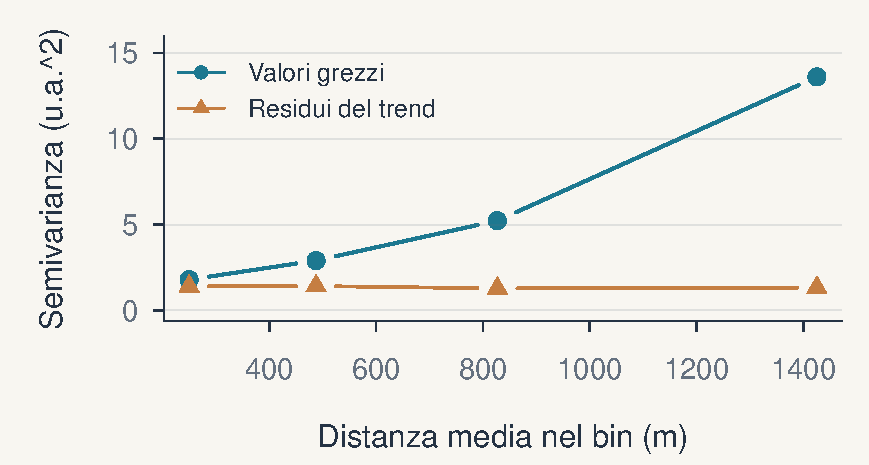
\includegraphics[width=9.85cm,height=5.25cm,keepaspectratio]{Risultati/Figure/24_semivariogramma.pdf}
\vspace{1.5mm}
\PSmall{Classi $(0,300]$, $(300,600]$, $(600,1000]$, $(1000,2500]$ m. L’ascissa è la distanza media delle coppie.}
\[\widehat\gamma_k=\frac{1}{2N_k}\sum_{(i,j)\in\mathcal P_k}(z_i-z_j)^2\]

\end{minipage}\end{lrbox}
\typeout{FULLBOX:073:PilotLeftBox:\the\ht\PilotLeftBox:\the\dp\PilotLeftBox}

\begin{lrbox}{\PilotRightBox}
\begin{minipage}[t]{7.55cm}\raggedright\color{Ink}\fontsize{11.3}{14.8}\selectfont
\PBody{Ogni classe contiene $N_k$ coppie. Il valore stimato è la media dei loro contributi, non il contributo della coppia alla distanza centrale.}
\vspace{2.5mm}
\PInfo{Numero e ampiezza delle classi controllano il compromesso fra dettaglio e stabilità descrittiva. Le classi finali non devono essere interpretate senza i conteggi.}
\PCode{R · medie per classe}{073_esempio.R}
\end{minipage}\end{lrbox}
\typeout{FULLBOX:073:PilotRightBox:\the\ht\PilotRightBox:\the\dp\PilotRightBox}

\begin{tikzpicture}[remember picture,overlay]
\PilotChrome{Il semivariogramma empirico raggruppa distanze}{VI · SEMIVARIANZA}{73}{Il semivariogramma empirico deve mostrare come sono costruite le classi di distanza.}
\node[anchor=north west,inner sep=0] at([xshift=.96cm,yshift=-2.13cm]current page.north west){\usebox{\PilotLeftBox}};
\node[anchor=north west,inner sep=0] at([xshift=11.52cm,yshift=-2.13cm]current page.north west){\usebox{\PilotRightBox}};
\node[anchor=north east,inner sep=0] at([xshift=17.65cm,yshift=-12.06cm]current page.north west){\color{Classical}\fontsize{7.7}{9.2}\selectfont\href{../../03_Notebook_svolti/M11_Locus/M11_N15.html}{M11\_N15 · notebook svolto}};
\end{tikzpicture}\end{frame}

\begin{frame}[plain]\hypertarget{slide74}{}
\bookmark[level=1,page=74]{Molte coppie non sono molte repliche indipendenti}
\begin{lrbox}{\TitleBox}
\begin{minipage}[t]{17.7cm}\raggedright\color{Ink}\fontsize{11.3}{14.8}\selectfont
\color{Navy}\bfseries\fontsize{20.6}{24.5}\selectfont Molte coppie non sono molte repliche indipendenti
\end{minipage}\end{lrbox}
\typeout{FULLBOX:074:TitleBox:\the\ht\TitleBox:\the\dp\TitleBox}

\begin{lrbox}{\RecallBox}
\begin{minipage}[t]{14.3cm}\raggedright\color{Ink}\fontsize{11.3}{14.8}\selectfont
\fontsize{10.3}{13.8}\selectfont 2016 coppie costruite da 64 siti non equivalgono a 2016 nuovi campioni indipendenti.
\end{minipage}\end{lrbox}
\typeout{FULLBOX:074:RecallBox:\the\ht\RecallBox:\the\dp\RecallBox}

\begin{lrbox}{\PilotLeftBox}
\begin{minipage}[t]{10.05cm}\raggedright\color{Ink}\fontsize{11.3}{14.8}\selectfont
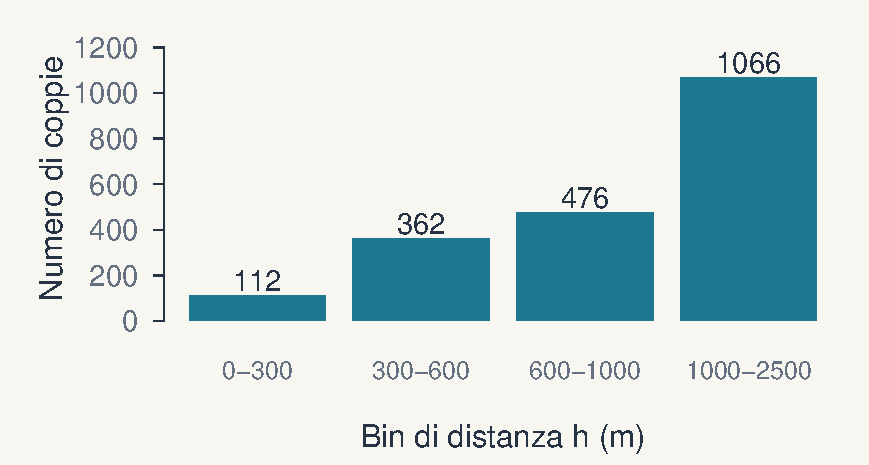
\includegraphics[width=9.85cm,height=5.25cm,keepaspectratio]{Risultati/Figure/25_numerosita_coppie.pdf}
\vspace{1.5mm}
\PSmall{I conteggi per classe sommano a 2016. Coppie non ordinate distinte possono condividere un sito.}

\end{minipage}\end{lrbox}
\typeout{FULLBOX:074:PilotLeftBox:\the\ht\PilotLeftBox:\the\dp\PilotLeftBox}

\begin{lrbox}{\PilotRightBox}
\begin{minipage}[t]{7.55cm}\raggedright\color{Ink}\fontsize{11.3}{14.8}\selectfont
\PBody{Le coppie $(i,j)$ e $(i,k)$ contengono la stessa osservazione $z_i$. I loro contributi possono quindi essere dipendenti.}
\vspace{2.5mm}
\PInfo{Non è giustificato trattare tutte le coppie come osservazioni indipendenti per ottenere intervalli stretti della curva.}
\PBody{Il conteggio delle coppie è utile per leggere la stabilità del riassunto. L’incertezza richiede un metodo coerente con la struttura spaziale.}
\vspace{2.5mm}

\end{minipage}\end{lrbox}
\typeout{FULLBOX:074:PilotRightBox:\the\ht\PilotRightBox:\the\dp\PilotRightBox}

\begin{tikzpicture}[remember picture,overlay]
\PilotChrome{Molte coppie non sono molte repliche indipendenti}{VI · SEMIVARIANZA}{74}{2016 coppie costruite da 64 siti non equivalgono a 2016 nuovi campioni indipendenti.}
\node[anchor=north west,inner sep=0] at([xshift=.96cm,yshift=-2.13cm]current page.north west){\usebox{\PilotLeftBox}};
\node[anchor=north west,inner sep=0] at([xshift=11.52cm,yshift=-2.13cm]current page.north west){\usebox{\PilotRightBox}};
\node[anchor=north east,inner sep=0] at([xshift=17.65cm,yshift=-12.06cm]current page.north west){\color{Classical}\fontsize{7.7}{9.2}\selectfont\href{../../03_Notebook_svolti/M11_Locus/M11_N15.html}{M11\_N15 · notebook svolto}};
\end{tikzpicture}\end{frame}

\begin{frame}[plain]\hypertarget{slide75}{}
\bookmark[level=1,page=75]{Semivarianza e covarianza sono collegate}
\begin{lrbox}{\TitleBox}
\begin{minipage}[t]{17.7cm}\raggedright\color{Ink}\fontsize{11.3}{14.8}\selectfont
\color{Navy}\bfseries\fontsize{20.6}{24.5}\selectfont Semivarianza e covarianza sono collegate
\end{minipage}\end{lrbox}
\typeout{FULLBOX:075:TitleBox:\the\ht\TitleBox:\the\dp\TitleBox}

\begin{lrbox}{\RecallBox}
\begin{minipage}[t]{14.3cm}\raggedright\color{Ink}\fontsize{11.3}{14.8}\selectfont
\fontsize{10.3}{13.8}\selectfont La relazione con la covarianza richiede ipotesi sul processo, non soltanto una formula applicata ai dati.
\end{minipage}\end{lrbox}
\typeout{FULLBOX:075:RecallBox:\the\ht\RecallBox:\the\dp\RecallBox}

\begin{lrbox}{\PilotLeftBox}
\begin{minipage}[t]{10.05cm}\raggedright\color{Ink}\fontsize{11.3}{14.8}\selectfont
\[\gamma(h)=\tfrac12\operatorname{Var}\{Z(s+h)-Z(s)\}\]
\[\gamma(h)=C(0)-C(h)\]
\PInfo{La seconda uguaglianza vale per un processo stazionario al secondo ordine con la stessa varianza nei due siti. In presenza di anisotropia h è un vettore.}

\end{minipage}\end{lrbox}
\typeout{FULLBOX:075:PilotLeftBox:\the\ht\PilotLeftBox:\the\dp\PilotLeftBox}

\begin{lrbox}{\PilotRightBox}
\begin{minipage}[t]{7.55cm}\raggedright\color{Ink}\fontsize{11.3}{14.8}\selectfont
\PBody{Se la covarianza diminuisce con la separazione, aumenta la variabilità delle differenze. La relazione collega una descrizione delle coppie a un modello probabilistico.}
\vspace{2.5mm}
\PBody{La media empirica delle differenze quadratiche stima questo oggetto quando le ipotesi sulla media e sugli incrementi sono adeguate.}
\vspace{2.5mm}

\end{minipage}\end{lrbox}
\typeout{FULLBOX:075:PilotRightBox:\the\ht\PilotRightBox:\the\dp\PilotRightBox}

\begin{tikzpicture}[remember picture,overlay]
\PilotChrome{Semivarianza e covarianza sono collegate}{VI · SEMIVARIANZA}{75}{La relazione con la covarianza richiede ipotesi sul processo, non soltanto una formula applicata ai dati.}
\node[anchor=north west,inner sep=0] at([xshift=.96cm,yshift=-2.13cm]current page.north west){\usebox{\PilotLeftBox}};
\node[anchor=north west,inner sep=0] at([xshift=11.52cm,yshift=-2.13cm]current page.north west){\usebox{\PilotRightBox}};
\end{tikzpicture}\end{frame}

\begin{frame}[plain]\hypertarget{slide76}{}
\bookmark[level=1,page=76]{La stazionarietà distingue media e dipendenza}
\begin{lrbox}{\TitleBox}
\begin{minipage}[t]{17.7cm}\raggedright\color{Ink}\fontsize{11.3}{14.8}\selectfont
\color{Navy}\bfseries\fontsize{20.6}{24.5}\selectfont La stazionarietà distingue media e dipendenza
\end{minipage}\end{lrbox}
\typeout{FULLBOX:076:TitleBox:\the\ht\TitleBox:\the\dp\TitleBox}

\begin{lrbox}{\RecallBox}
\begin{minipage}[t]{14.3cm}\raggedright\color{Ink}\fontsize{11.3}{14.8}\selectfont
\fontsize{10.3}{13.8}\selectfont Il modello di semivarianza deve essere coerente con ciò che è stato rimosso o mantenuto nella media.
\end{minipage}\end{lrbox}
\typeout{FULLBOX:076:RecallBox:\the\ht\RecallBox:\the\dp\RecallBox}

\begin{lrbox}{\PilotLeftBox}
\begin{minipage}[t]{10.05cm}\raggedright\color{Ink}\fontsize{11.3}{14.8}\selectfont
{\fontsize{10.2}{13.1}\selectfont\renewcommand{\arraystretch}{1.45}\begin{tabular}{@{}p{3.1cm}p{5.9cm}@{}}\toprule
\textbf{Ipotesi} & \textbf{Contenuto}\\\midrule
Secondo ordine & $\mathbb E[Z(s)]=\mu$, covarianza dipendente dallo spostamento\\
Intrinseca & Incrementi a media zero e varianza dipendente dallo spostamento\\
Isotropia & Dipendenza dalla lunghezza dello spostamento\\
Trend spaziale & Media che varia con la posizione\\
\bottomrule\end{tabular}}

\end{minipage}\end{lrbox}
\typeout{FULLBOX:076:PilotLeftBox:\the\ht\PilotLeftBox:\the\dp\PilotLeftBox}

\begin{lrbox}{\PilotRightBox}
\begin{minipage}[t]{7.55cm}\raggedright\color{Ink}\fontsize{11.3}{14.8}\selectfont
\PBody{La stazionarietà intrinseca è una condizione diversa, più debole di quella al secondo ordine. Non impone l’esistenza di una covarianza stazionaria finita.}
\vspace{2.5mm}
\PInfo{Nel caso guida il gradiente della media rende prudente interpretare la curva grezza. Un aumento della semivarianza può riflettere anche quel gradiente.}
\PBody{Prima di adattare un modello, valutiamo media, direzione, supporto e copertura delle coppie.}
\vspace{2.5mm}

\end{minipage}\end{lrbox}
\typeout{FULLBOX:076:PilotRightBox:\the\ht\PilotRightBox:\the\dp\PilotRightBox}

\begin{tikzpicture}[remember picture,overlay]
\PilotChrome{La stazionarietà distingue media e dipendenza}{VI · SEMIVARIANZA}{76}{Il modello di semivarianza deve essere coerente con ciò che è stato rimosso o mantenuto nella media.}
\node[anchor=north west,inner sep=0] at([xshift=.96cm,yshift=-2.13cm]current page.north west){\usebox{\PilotLeftBox}};
\node[anchor=north west,inner sep=0] at([xshift=11.52cm,yshift=-2.13cm]current page.north west){\usebox{\PilotRightBox}};
\end{tikzpicture}\end{frame}

\begin{frame}[plain]\hypertarget{slide77}{}
\bookmark[level=1,page=77]{L’isotropia è un’ipotesi aggiuntiva}
\begin{lrbox}{\TitleBox}
\begin{minipage}[t]{17.7cm}\raggedright\color{Ink}\fontsize{11.3}{14.8}\selectfont
\color{Navy}\bfseries\fontsize{20.6}{24.5}\selectfont L’isotropia è un’ipotesi aggiuntiva
\end{minipage}\end{lrbox}
\typeout{FULLBOX:077:TitleBox:\the\ht\TitleBox:\the\dp\TitleBox}

\begin{lrbox}{\RecallBox}
\begin{minipage}[t]{14.3cm}\raggedright\color{Ink}\fontsize{11.3}{14.8}\selectfont
\fontsize{10.3}{13.8}\selectfont L’assenza della direzione dal grafico non dimostra che il processo sia isotropo.
\end{minipage}\end{lrbox}
\typeout{FULLBOX:077:RecallBox:\the\ht\RecallBox:\the\dp\RecallBox}

\begin{lrbox}{\FullWideBox}
\begin{minipage}[t]{18.1cm}\raggedright\color{Ink}\fontsize{11.3}{14.8}\selectfont
\centering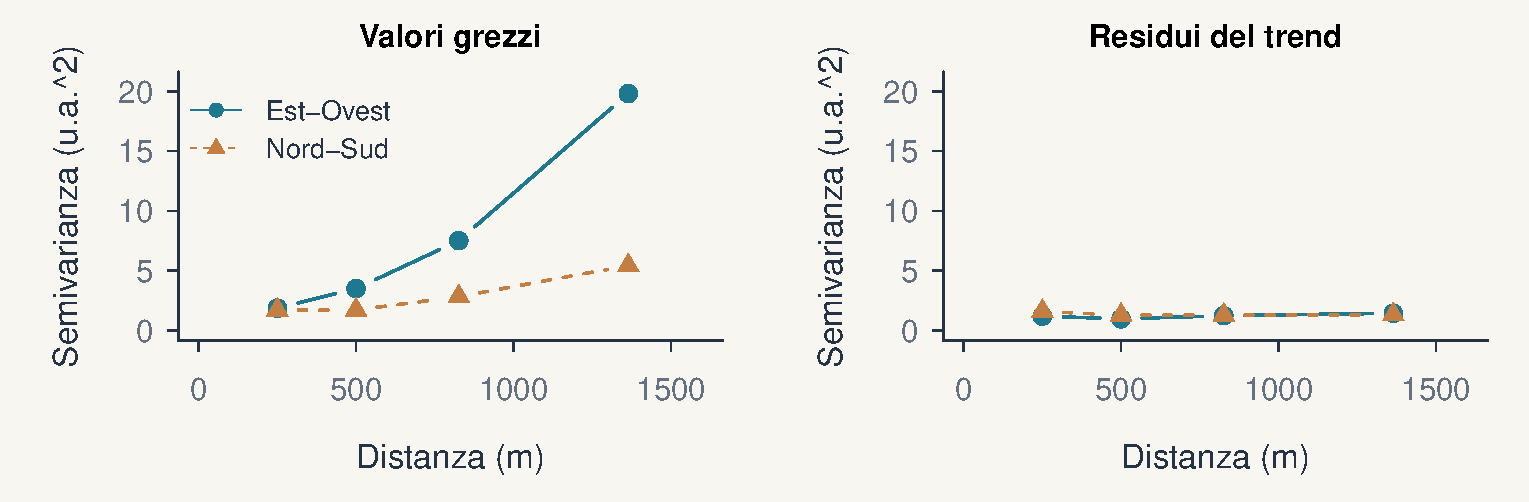
\includegraphics[width=18.05cm,height=5.8cm,keepaspectratio]{Risultati/Figure/26_direzionali.pdf}
\end{minipage}\end{lrbox}
\typeout{FULLBOX:077:FullWideBox:\the\ht\FullWideBox:\the\dp\FullWideBox}

\begin{lrbox}{\PilotRightBox}
\begin{minipage}[t]{18.1cm}\raggedright\color{Ink}\fontsize{11.3}{14.8}\selectfont
\PBody{Le coppie sono raggruppate per distanza e direzione con tolleranze dichiarate nei calcoli. Un riassunto omnidirezionale può nascondere differenze orientate. Trend, numerosità e geometria del campione incidono sul confronto: la differenza fra curve non basta da sola a identificare anisotropia del processo.}
\end{minipage}\end{lrbox}
\typeout{FULLBOX:077:PilotRightBox:\the\ht\PilotRightBox:\the\dp\PilotRightBox}

\begin{tikzpicture}[remember picture,overlay]
\PilotChrome{L’isotropia è un’ipotesi aggiuntiva}{VI · SEMIVARIANZA}{77}{L’assenza della direzione dal grafico non dimostra che il processo sia isotropo.}
\node[anchor=north west,inner sep=0] at([xshift=.96cm,yshift=-2.13cm]current page.north west){\usebox{\FullWideBox}};
\node[anchor=north west,inner sep=0] at([xshift=.96cm,yshift=-8.25cm]current page.north west){\usebox{\PilotRightBox}};
\end{tikzpicture}\end{frame}

\begin{frame}[plain]\hypertarget{slide78}{}
\bookmark[level=1,page=78]{Nugget, sill e range dipendono dal modello}
\begin{lrbox}{\TitleBox}
\begin{minipage}[t]{17.7cm}\raggedright\color{Ink}\fontsize{11.3}{14.8}\selectfont
\color{Navy}\bfseries\fontsize{20.6}{24.5}\selectfont Nugget, sill e range dipendono dal modello
\end{minipage}\end{lrbox}
\typeout{FULLBOX:078:TitleBox:\the\ht\TitleBox:\the\dp\TitleBox}

\begin{lrbox}{\RecallBox}
\begin{minipage}[t]{14.3cm}\raggedright\color{Ink}\fontsize{11.3}{14.8}\selectfont
\fontsize{10.3}{13.8}\selectfont I nomi dei parametri devono accompagnare la formula che ne definisce il significato.
\end{minipage}\end{lrbox}
\typeout{FULLBOX:078:RecallBox:\the\ht\RecallBox:\the\dp\RecallBox}

\begin{lrbox}{\PilotLeftBox}
\begin{minipage}[t]{10.05cm}\raggedright\color{Ink}\fontsize{11.3}{14.8}\selectfont
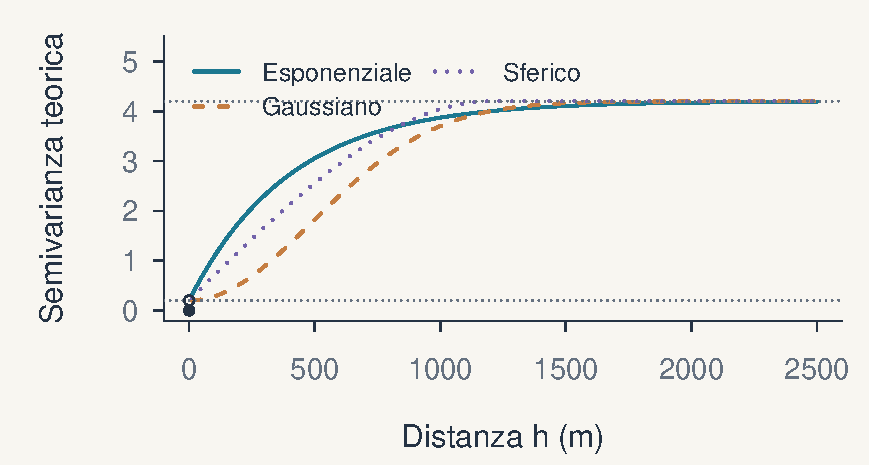
\includegraphics[width=9.85cm,height=5.25cm,keepaspectratio]{Risultati/Figure/27_modelli_variogramma.pdf}
\vspace{1.5mm}
\PSmall{Modelli teorici illustrativi con parametri dichiarati; non sono adattamenti automatici ai 64 valori.}

\end{minipage}\end{lrbox}
\typeout{FULLBOX:078:PilotLeftBox:\the\ht\PilotLeftBox:\the\dp\PilotLeftBox}

\begin{lrbox}{\PilotRightBox}
\begin{minipage}[t]{7.55cm}\raggedright\color{Ink}\fontsize{11.3}{14.8}\selectfont
\PBody{Il nugget descrive un salto all’origine, interpretabile secondo il modello come errore di misura o variazione a scale non risolte. Il sill è il livello limite quando esiste.}
\vspace{2.5mm}
\PInfo{Per il modello esponenziale la scala a non è un range finito: a $3a$ si raggiunge circa il 95\% del sill strutturale.}
\PSmall{Un modello sferico raggiunge il sill a distanza finita. Specificare sempre la convenzione usata dal software.}

\end{minipage}\end{lrbox}
\typeout{FULLBOX:078:PilotRightBox:\the\ht\PilotRightBox:\the\dp\PilotRightBox}

\begin{tikzpicture}[remember picture,overlay]
\PilotChrome{Nugget, sill e range dipendono dal modello}{VI · SEMIVARIANZA}{78}{I nomi dei parametri devono accompagnare la formula che ne definisce il significato.}
\node[anchor=north west,inner sep=0] at([xshift=.96cm,yshift=-2.13cm]current page.north west){\usebox{\PilotLeftBox}};
\node[anchor=north west,inner sep=0] at([xshift=11.52cm,yshift=-2.13cm]current page.north west){\usebox{\PilotRightBox}};
\end{tikzpicture}\end{frame}

\begin{frame}[plain]\hypertarget{slide79}{}
\bookmark[level=1,page=79]{Il nugget cambia il bersaglio della previsione}
\begin{lrbox}{\TitleBox}
\begin{minipage}[t]{17.7cm}\raggedright\color{Ink}\fontsize{11.3}{14.8}\selectfont
\color{Navy}\bfseries\fontsize{20.6}{24.5}\selectfont Il nugget cambia il bersaglio della previsione
\end{minipage}\end{lrbox}
\typeout{FULLBOX:079:TitleBox:\the\ht\TitleBox:\the\dp\TitleBox}

\begin{lrbox}{\RecallBox}
\begin{minipage}[t]{14.3cm}\raggedright\color{Ink}\fontsize{11.3}{14.8}\selectfont
\fontsize{10.3}{13.8}\selectfont La varianza predittiva dipende dal fatto che il bersaglio sia un campo latente o una nuova misura.
\end{minipage}\end{lrbox}
\typeout{FULLBOX:079:RecallBox:\the\ht\RecallBox:\the\dp\RecallBox}

\begin{lrbox}{\PilotLeftBox}
\begin{minipage}[t]{10.05cm}\raggedright\color{Ink}\fontsize{11.3}{14.8}\selectfont
\[Y(s)=X(s)+\eta(s),\qquad \operatorname{Var}\{\eta(s)\}=\tau^2\]
\[\operatorname{Cov}\{Y(s_i),Y(s_j)\}=C_X(s_i,s_j)+\tau^2\mathbf1(i=j)\]
\PInfo{La formula assume errori di misura indipendenti fra osservazioni e indipendenti dal campo latente X. Sono ipotesi del modello.}

\end{minipage}\end{lrbox}
\typeout{FULLBOX:079:PilotLeftBox:\the\ht\PilotLeftBox:\the\dp\PilotLeftBox}

\begin{lrbox}{\PilotRightBox}
\begin{minipage}[t]{7.55cm}\raggedright\color{Ink}\fontsize{11.3}{14.8}\selectfont
\PBody{Prevedere il campo latente X in un sito non equivale a prevedere una nuova misura Y nello stesso sito. La seconda include una nuova componente di errore.}
\vspace{2.5mm}
\PBody{Per repliche nello stesso luogo bisogna distinguere identità del sito e identità dell’osservazione. La covarianza dell’errore non si deduce dalla sola distanza.}
\vspace{2.5mm}

\end{minipage}\end{lrbox}
\typeout{FULLBOX:079:PilotRightBox:\the\ht\PilotRightBox:\the\dp\PilotRightBox}

\begin{tikzpicture}[remember picture,overlay]
\PilotChrome{Il nugget cambia il bersaglio della previsione}{VI · SEMIVARIANZA}{79}{La varianza predittiva dipende dal fatto che il bersaglio sia un campo latente o una nuova misura.}
\node[anchor=north west,inner sep=0] at([xshift=.96cm,yshift=-2.13cm]current page.north west){\usebox{\PilotLeftBox}};
\node[anchor=north west,inner sep=0] at([xshift=11.52cm,yshift=-2.13cm]current page.north west){\usebox{\PilotRightBox}};
\end{tikzpicture}\end{frame}

\begin{frame}[plain]\hypertarget{slide80}{}
\bookmark[level=1,page=80]{Adattare una curva richiede un modello valido}
\begin{lrbox}{\TitleBox}
\begin{minipage}[t]{17.7cm}\raggedright\color{Ink}\fontsize{11.3}{14.8}\selectfont
\color{Navy}\bfseries\fontsize{20.6}{24.5}\selectfont Adattare una curva richiede un modello valido
\end{minipage}\end{lrbox}
\typeout{FULLBOX:080:TitleBox:\the\ht\TitleBox:\the\dp\TitleBox}

\begin{lrbox}{\RecallBox}
\begin{minipage}[t]{14.3cm}\raggedright\color{Ink}\fontsize{11.3}{14.8}\selectfont
\fontsize{10.3}{13.8}\selectfont Il modello deve essere valido e stimato con informazioni compatibili con la verifica previsionale.
\end{minipage}\end{lrbox}
\typeout{FULLBOX:080:RecallBox:\the\ht\RecallBox:\the\dp\RecallBox}

\begin{lrbox}{\PilotLeftBox}
\begin{minipage}[t]{10.05cm}\raggedright\color{Ink}\fontsize{11.3}{14.8}\selectfont
\[\sum_k q_k\{\widehat\gamma_k-\gamma(h_k;\theta)\}^2\]
{\fontsize{10.2}{13.1}\selectfont\renewcommand{\arraystretch}{1.45}\begin{tabular}{@{}p{3.4cm}p{5.6cm}@{}}\toprule
\textbf{Scelta} & \textbf{Controllo}\\\midrule
Famiglia di modelli & Validità della covarianza o del variogramma\\
Pesi delle classi & Criterio dichiarato, conteggi disponibili\\
Parametri & Vincoli e convenzioni esplicite\\
Dominio di stima & Solo dati ammessi dal protocollo\\
\bottomrule\end{tabular}}

\end{minipage}\end{lrbox}
\typeout{FULLBOX:080:PilotLeftBox:\the\ht\PilotLeftBox:\the\dp\PilotLeftBox}

\begin{lrbox}{\PilotRightBox}
\begin{minipage}[t]{7.55cm}\raggedright\color{Ink}\fontsize{11.3}{14.8}\selectfont
\PBody{Un criterio pesato può descrivere l’adattamento della curva. Non rende indipendenti le classi e non garantisce un’inferenza corretta sui parametri.}
\vspace{2.5mm}
\PInfo{Una curva visivamente liscia non è necessariamente una covarianza valida. Il sistema di kriging richiede un modello matematicamente ammissibile.}
\PBody{Nel piccolo esempio di kriging useremo una covarianza gaussiana dichiarata, così da isolare e verificare il sistema dei pesi.}
\vspace{2.5mm}

\end{minipage}\end{lrbox}
\typeout{FULLBOX:080:PilotRightBox:\the\ht\PilotRightBox:\the\dp\PilotRightBox}

\begin{tikzpicture}[remember picture,overlay]
\PilotChrome{Adattare una curva richiede un modello valido}{VI · SEMIVARIANZA}{80}{Il modello deve essere valido e stimato con informazioni compatibili con la verifica previsionale.}
\node[anchor=north west,inner sep=0] at([xshift=.96cm,yshift=-2.13cm]current page.north west){\usebox{\PilotLeftBox}};
\node[anchor=north west,inner sep=0] at([xshift=11.52cm,yshift=-2.13cm]current page.north west){\usebox{\PilotRightBox}};
\end{tikzpicture}\end{frame}

\begin{frame}[plain]\hypertarget{slide81}{}
\bookmark[level=1,page=81]{Laboratorio: dalle coppie alle ipotesi}
\begin{lrbox}{\TitleBox}
\begin{minipage}[t]{17.7cm}\raggedright\color{Ink}\fontsize{11.3}{14.8}\selectfont
\color{Navy}\bfseries\fontsize{20.6}{24.5}\selectfont Laboratorio: dalle coppie alle ipotesi
\end{minipage}\end{lrbox}
\typeout{FULLBOX:081:TitleBox:\the\ht\TitleBox:\the\dp\TitleBox}

\begin{lrbox}{\RecallBox}
\begin{minipage}[t]{14.3cm}\raggedright\color{Ink}\fontsize{11.3}{14.8}\selectfont
\fontsize{10.3}{13.8}\selectfont Un semivariogramma utile unisce curva, conteggi, supporto e ipotesi sul processo.
\end{minipage}\end{lrbox}
\typeout{FULLBOX:081:RecallBox:\the\ht\RecallBox:\the\dp\RecallBox}

\begin{lrbox}{\PilotLeftBox}
\begin{minipage}[t]{10.05cm}\raggedright\color{Ink}\fontsize{11.3}{14.8}\selectfont
\PLab{https://marzione00.github.io/Lab_Geo/\#laboratorio/m11-variogramma}{Esperimento online · coppie e semivariogramma}
{\fontsize{10.2}{13.1}\selectfont\renewcommand{\arraystretch}{1.45}\begin{tabular}{@{}p{4.0cm}p{5.0cm}@{}}\toprule
\textbf{Consegna N15} & \textbf{Controllo}\\\midrule
Tabella delle coppie & 2016 coppie, senza diagonale\\
Classi di distanza & Estremi e inclusione del bordo\\
Curva empirica & Distanza media, semivarianza, conteggi\\
Interpretazione & Trend, direzione e dipendenza fra coppie\\
Modello eventuale & Formula, parametri e dominio di validità\\
\bottomrule\end{tabular}}

\end{minipage}\end{lrbox}
\typeout{FULLBOX:081:PilotLeftBox:\the\ht\PilotLeftBox:\the\dp\PilotLeftBox}

\begin{lrbox}{\PilotRightBox}
\begin{minipage}[t]{7.55cm}\raggedright\color{Ink}\fontsize{11.3}{14.8}\selectfont
\PBody{Il grafico deve rendere visibili le scale in metri e in $(\mathrm{u.a.})^2$. La discussione precisa ciò che il campionamento permette di osservare.}
\vspace{2.5mm}
\PInfo{Più classi non aggiungono dati. Un modello della dipendenza richiede anche una copertura adeguata di distanze e direzioni.}
\PBody{Passiamo quindi dalla geometria delle coppie al disegno del campionamento.}
\vspace{2.5mm}

\end{minipage}\end{lrbox}
\typeout{FULLBOX:081:PilotRightBox:\the\ht\PilotRightBox:\the\dp\PilotRightBox}

\begin{tikzpicture}[remember picture,overlay]
\PilotChrome{Laboratorio: dalle coppie alle ipotesi}{VI · SEMIVARIANZA}{81}{Un semivariogramma utile unisce curva, conteggi, supporto e ipotesi sul processo.}
\node[anchor=north west,inner sep=0] at([xshift=.96cm,yshift=-2.13cm]current page.north west){\usebox{\PilotLeftBox}};
\node[anchor=north west,inner sep=0] at([xshift=11.52cm,yshift=-2.13cm]current page.north west){\usebox{\PilotRightBox}};
\node[anchor=north east,inner sep=0] at([xshift=17.65cm,yshift=-12.06cm]current page.north west){\color{Classical}\fontsize{7.7}{9.2}\selectfont\href{../../03_Notebook_svolti/M11_Locus/M11_N15.html}{M11\_N15 · notebook svolto}};
\end{tikzpicture}\end{frame}

\begin{frame}[plain]\hypertarget{slide82}{}
\bookmark[level=0,page=82]{VII · COPERTURA DEL CAMPIONE}
\bookmark[level=1,page=82]{Il campione deve rappresentare un dominio}
\begin{lrbox}{\TitleBox}
\begin{minipage}[t]{17.7cm}\raggedright\color{Ink}\fontsize{11.3}{14.8}\selectfont
\color{Navy}\bfseries\fontsize{20.6}{24.5}\selectfont Il campione deve rappresentare un dominio
\end{minipage}\end{lrbox}
\typeout{FULLBOX:082:TitleBox:\the\ht\TitleBox:\the\dp\TitleBox}

\begin{lrbox}{\RecallBox}
\begin{minipage}[t]{14.3cm}\raggedright\color{Ink}\fontsize{11.3}{14.8}\selectfont
\fontsize{10.3}{13.8}\selectfont La rappresentatività dipende da come i siti sono stati scelti e dalla popolazione a cui si vuole riferire il risultato.
\end{minipage}\end{lrbox}
\typeout{FULLBOX:082:RecallBox:\the\ht\RecallBox:\the\dp\RecallBox}

\begin{lrbox}{\PilotLeftBox}
\begin{minipage}[t]{10.05cm}\raggedright\color{Ink}\fontsize{11.3}{14.8}\selectfont
{\fontsize{10.2}{13.1}\selectfont\renewcommand{\arraystretch}{1.45}\begin{tabular}{@{}p{3.2cm}p{5.8cm}@{}}\toprule
\textbf{Scelta} & \textbf{Domanda da risolvere}\\\midrule
Dominio & Quale territorio interessa la conclusione?\\
Unità & Che cosa costituisce un campione?\\
Accessibilità & Quali aree sono più facili da osservare?\\
Distanze & Quali scale di variazione sono coperte?\\
Bersaglio & Media dei siti, media areale o previsione?\\
\bottomrule\end{tabular}}

\end{minipage}\end{lrbox}
\typeout{FULLBOX:082:PilotLeftBox:\the\ht\PilotLeftBox:\the\dp\PilotLeftBox}

\begin{lrbox}{\PilotRightBox}
\begin{minipage}[t]{7.55cm}\raggedright\color{Ink}\fontsize{11.3}{14.8}\selectfont
\PBody{La posizione dei campioni non è un semplice dettaglio del file. Determina quali parti del territorio e quali distanze sono rappresentate.}
\vspace{2.5mm}
\PInfo{Un numero elevato di osservazioni vicino a una strada può descrivere bene quel corridoio e male il resto del dominio.}
\PBody{La qualità del campione va discussa rispetto al bersaglio dell’analisi.}
\vspace{2.5mm}

\end{minipage}\end{lrbox}
\typeout{FULLBOX:082:PilotRightBox:\the\ht\PilotRightBox:\the\dp\PilotRightBox}

\begin{tikzpicture}[remember picture,overlay]
\PilotChrome{Il campione deve rappresentare un dominio}{VII · COPERTURA DEL CAMPIONE}{82}{La rappresentatività dipende da come i siti sono stati scelti e dalla popolazione a cui si vuole riferire il risultato.}
\node[anchor=north west,inner sep=0] at([xshift=.96cm,yshift=-2.13cm]current page.north west){\usebox{\PilotLeftBox}};
\node[anchor=north west,inner sep=0] at([xshift=11.52cm,yshift=-2.13cm]current page.north west){\usebox{\PilotRightBox}};
\end{tikzpicture}\end{frame}

\begin{frame}[plain]\hypertarget{slide83}{}
\bookmark[level=1,page=83]{Campionare lungo una strada seleziona un’area}
\begin{lrbox}{\TitleBox}
\begin{minipage}[t]{17.7cm}\raggedright\color{Ink}\fontsize{11.3}{14.8}\selectfont
\color{Navy}\bfseries\fontsize{20.6}{24.5}\selectfont Campionare lungo una strada seleziona un’area
\end{minipage}\end{lrbox}
\typeout{FULLBOX:083:TitleBox:\the\ht\TitleBox:\the\dp\TitleBox}

\begin{lrbox}{\RecallBox}
\begin{minipage}[t]{14.3cm}\raggedright\color{Ink}\fontsize{11.3}{14.8}\selectfont
\fontsize{10.3}{13.8}\selectfont La facilità di accesso può rendere il campione spazialmente selettivo.
\end{minipage}\end{lrbox}
\typeout{FULLBOX:083:RecallBox:\the\ht\RecallBox:\the\dp\RecallBox}

\begin{lrbox}{\PilotLeftBox}
\begin{minipage}[t]{10.05cm}\raggedright\color{Ink}\fontsize{11.3}{14.8}\selectfont
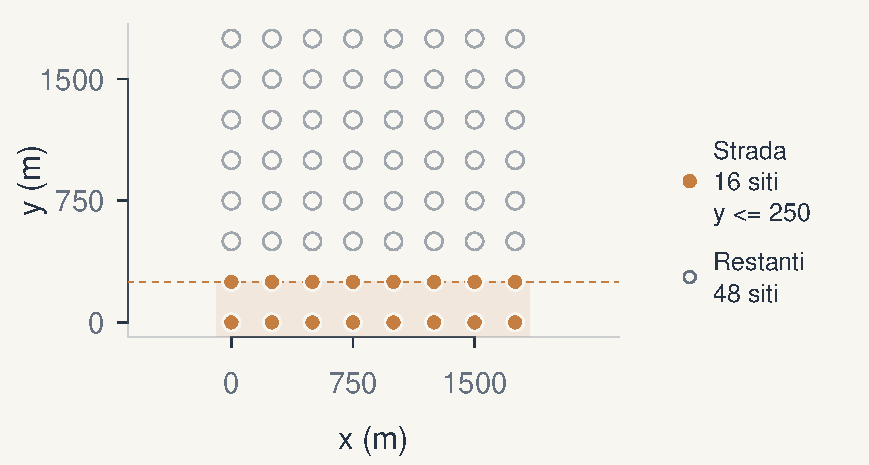
\includegraphics[width=9.85cm,height=5.25cm,keepaspectratio]{Risultati/Figure/28_strada_campione.pdf}
\vspace{1.5mm}
\PSmall{Campione di convenienza: i 16 siti con $y\le250$ m. Gli altri 48 siti descrivono il territorio escluso.}

\end{minipage}\end{lrbox}
\typeout{FULLBOX:083:PilotLeftBox:\the\ht\PilotLeftBox:\the\dp\PilotLeftBox}

\begin{lrbox}{\PilotRightBox}
\begin{minipage}[t]{7.55cm}\raggedright\color{Ink}\fontsize{11.3}{14.8}\selectfont
\PBody{La media del corridoio è 15,87 u.a.; quella dell’intera griglia è 17,19 u.a. La differenza è -1,32 u.a.}
\vspace{2.5mm}
\PInfo{In un’indagine reale il valore medio del territorio escluso non sarebbe noto. Il dataset completo permette qui di osservare l’effetto della selezione.}
\PCode{R · confronto descrittivo}{083_esempio.R}
\end{minipage}\end{lrbox}
\typeout{FULLBOX:083:PilotRightBox:\the\ht\PilotRightBox:\the\dp\PilotRightBox}

\begin{tikzpicture}[remember picture,overlay]
\PilotChrome{Campionare lungo una strada seleziona un’area}{VII · COPERTURA DEL CAMPIONE}{83}{La facilità di accesso può rendere il campione spazialmente selettivo.}
\node[anchor=north west,inner sep=0] at([xshift=.96cm,yshift=-2.13cm]current page.north west){\usebox{\PilotLeftBox}};
\node[anchor=north west,inner sep=0] at([xshift=11.52cm,yshift=-2.13cm]current page.north west){\usebox{\PilotRightBox}};
\node[anchor=north east,inner sep=0] at([xshift=17.65cm,yshift=-12.06cm]current page.north west){\color{Classical}\fontsize{7.7}{9.2}\selectfont\href{../../03_Notebook_svolti/M11_Locus/M11_N16.html}{M11\_N16 · notebook svolto}};
\end{tikzpicture}\end{frame}

\begin{frame}[plain]\hypertarget{slide84}{}
\bookmark[level=1,page=84]{La copertura richiede una misura geografica}
\begin{lrbox}{\TitleBox}
\begin{minipage}[t]{17.7cm}\raggedright\color{Ink}\fontsize{11.3}{14.8}\selectfont
\color{Navy}\bfseries\fontsize{20.6}{24.5}\selectfont La copertura richiede una misura geografica
\end{minipage}\end{lrbox}
\typeout{FULLBOX:084:TitleBox:\the\ht\TitleBox:\the\dp\TitleBox}

\begin{lrbox}{\RecallBox}
\begin{minipage}[t]{14.3cm}\raggedright\color{Ink}\fontsize{11.3}{14.8}\selectfont
\fontsize{10.3}{13.8}\selectfont Il numero dei siti deve essere letto insieme alla loro distribuzione sul dominio.
\end{minipage}\end{lrbox}
\typeout{FULLBOX:084:RecallBox:\the\ht\RecallBox:\the\dp\RecallBox}

\begin{lrbox}{\PilotLeftBox}
\begin{minipage}[t]{10.05cm}\raggedright\color{Ink}\fontsize{11.3}{14.8}\selectfont
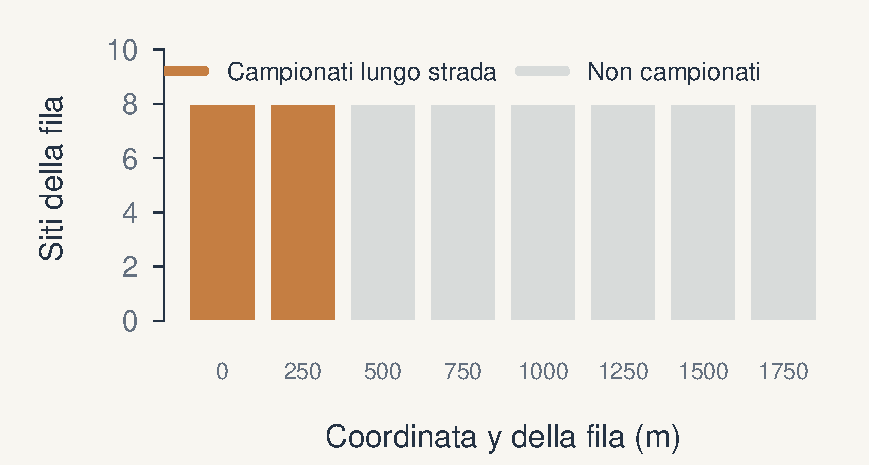
\includegraphics[width=9.85cm,height=5.25cm,keepaspectratio]{Risultati/Figure/29_copertura.pdf}
\vspace{1.5mm}
\PSmall{La copertura dipende dalla distribuzione dei siti e dalle distanze dalle aree non campionate.}

\end{minipage}\end{lrbox}
\typeout{FULLBOX:084:PilotLeftBox:\the\ht\PilotLeftBox:\the\dp\PilotLeftBox}

\begin{lrbox}{\PilotRightBox}
\begin{minipage}[t]{7.55cm}\raggedright\color{Ink}\fontsize{11.3}{14.8}\selectfont
\PBody{Conteggio, estensione e distanza dal campione più vicino descrivono aspetti diversi. Una nuvola densa in un angolo può lasciare una vasta regione scoperta.}
\vspace{2.5mm}
\PInfo{La distanza al sito più vicino è una misura geometrica, non una stima completa dell’errore di previsione. La relazione con l’errore dipende dal fenomeno e dal modello.}
\PBody{Per progettare nuovi campioni, consideriamo anche direzioni, litologie e accessibilità.}
\vspace{2.5mm}

\end{minipage}\end{lrbox}
\typeout{FULLBOX:084:PilotRightBox:\the\ht\PilotRightBox:\the\dp\PilotRightBox}

\begin{tikzpicture}[remember picture,overlay]
\PilotChrome{La copertura richiede una misura geografica}{VII · COPERTURA DEL CAMPIONE}{84}{Il numero dei siti deve essere letto insieme alla loro distribuzione sul dominio.}
\node[anchor=north west,inner sep=0] at([xshift=.96cm,yshift=-2.13cm]current page.north west){\usebox{\PilotLeftBox}};
\node[anchor=north west,inner sep=0] at([xshift=11.52cm,yshift=-2.13cm]current page.north west){\usebox{\PilotRightBox}};
\node[anchor=north east,inner sep=0] at([xshift=17.65cm,yshift=-12.06cm]current page.north west){\color{Classical}\fontsize{7.7}{9.2}\selectfont\href{../../03_Notebook_svolti/M11_Locus/M11_N16.html}{M11\_N16 · notebook svolto}};
\end{tikzpicture}\end{frame}

\begin{frame}[plain]\hypertarget{slide85}{}
\bookmark[level=1,page=85]{Bilanciare gli strati rende esplicito il disegno}
\begin{lrbox}{\TitleBox}
\begin{minipage}[t]{17.7cm}\raggedright\color{Ink}\fontsize{11.3}{14.8}\selectfont
\color{Navy}\bfseries\fontsize{20.6}{24.5}\selectfont Bilanciare gli strati rende esplicito il disegno
\end{minipage}\end{lrbox}
\typeout{FULLBOX:085:TitleBox:\the\ht\TitleBox:\the\dp\TitleBox}

\begin{lrbox}{\RecallBox}
\begin{minipage}[t]{14.3cm}\raggedright\color{Ink}\fontsize{11.3}{14.8}\selectfont
\fontsize{10.3}{13.8}\selectfont Il disegno chiarisce quali unità possono entrare nel campione e con quale peso.
\end{minipage}\end{lrbox}
\typeout{FULLBOX:085:RecallBox:\the\ht\RecallBox:\the\dp\RecallBox}

\begin{lrbox}{\PilotLeftBox}
\begin{minipage}[t]{10.05cm}\raggedright\color{Ink}\fontsize{11.3}{14.8}\selectfont
\begin{tikzpicture}[x=1cm,y=1cm]
\path[use as bounding box](-.1,-.15) rectangle(9.7,5.25);
\draw[pAxis](1,.4)--(8.7,.4)node[right,pNote]{$x$};
\draw[pAxis](1,.4)--(1,5.0)node[above,pNote]{$y$};
\fill[GeoA!8](1.2,.6)rectangle(5.7,4.8);
\fill[GeoB!12](5.7,.6)rectangle(8.4,4.8);
\draw[GeoB,dashed](5.7,.55)--(5.7,4.9);
\fill[GeoA](1.7,0.9)circle(2.7pt);
\fill[GeoA](3.7,0.9)circle(2.7pt);
\fill[GeoB](5.7,0.9)circle(2.7pt);
\fill[GeoB](7.7,0.9)circle(2.7pt);
\fill[GeoA](1.7,2.0)circle(2.7pt);
\fill[GeoA](3.7,2.0)circle(2.7pt);
\fill[GeoB](5.7,2.0)circle(2.7pt);
\fill[GeoB](7.7,2.0)circle(2.7pt);
\fill[GeoA](1.7,3.1)circle(2.7pt);
\fill[GeoA](3.7,3.1)circle(2.7pt);
\fill[GeoB](5.7,3.1)circle(2.7pt);
\fill[GeoB](7.7,3.1)circle(2.7pt);
\fill[GeoA](1.7,4.2)circle(2.7pt);
\fill[GeoA](3.7,4.2)circle(2.7pt);
\fill[GeoB](5.7,4.2)circle(2.7pt);
\fill[GeoB](7.7,4.2)circle(2.7pt);
\end{tikzpicture}
\PSmall{Il disegno documenta probabilità di inclusione, definizione degli strati oppure passo e origine della griglia, secondo la procedura adottata.}

\end{minipage}\end{lrbox}
\typeout{FULLBOX:085:PilotLeftBox:\the\ht\PilotLeftBox:\the\dp\PilotLeftBox}

\begin{lrbox}{\PilotRightBox}
\begin{minipage}[t]{7.55cm}\raggedright\color{Ink}\fontsize{11.3}{14.8}\selectfont
\PBody{Una stratificazione può garantire osservazioni in zone scientificamente diverse. La ripartizione del campione deve essere collegata al bersaglio e ai costi.}
\vspace{2.5mm}
\PInfo{Un’allocazione uguale per strato facilita alcuni confronti. Per una media dell’intero territorio possono servire pesi proporzionali alle aree o alle probabilità di inclusione.}
\PBody{La griglia del modulo è una costruzione didattica, non una garanzia generale contro distorsioni del campionamento.}
\vspace{2.5mm}

\end{minipage}\end{lrbox}
\typeout{FULLBOX:085:PilotRightBox:\the\ht\PilotRightBox:\the\dp\PilotRightBox}

\begin{tikzpicture}[remember picture,overlay]
\PilotChrome{Bilanciare gli strati rende esplicito il disegno}{VII · COPERTURA DEL CAMPIONE}{85}{Il disegno chiarisce quali unità possono entrare nel campione e con quale peso.}
\node[anchor=north west,inner sep=0] at([xshift=.96cm,yshift=-2.13cm]current page.north west){\usebox{\PilotLeftBox}};
\node[anchor=north west,inner sep=0] at([xshift=11.52cm,yshift=-2.13cm]current page.north west){\usebox{\PilotRightBox}};
\end{tikzpicture}\end{frame}

\begin{frame}[plain]\hypertarget{slide86}{}
\bookmark[level=1,page=86]{Con blocchi bilanciati le due medie coincidono}
\begin{lrbox}{\TitleBox}
\begin{minipage}[t]{17.7cm}\raggedright\color{Ink}\fontsize{11.3}{14.8}\selectfont
\color{Navy}\bfseries\fontsize{20.6}{24.5}\selectfont Con blocchi bilanciati le due medie coincidono
\end{minipage}\end{lrbox}
\typeout{FULLBOX:086:TitleBox:\the\ht\TitleBox:\the\dp\TitleBox}

\begin{lrbox}{\RecallBox}
\begin{minipage}[t]{14.3cm}\raggedright\color{Ink}\fontsize{11.3}{14.8}\selectfont
\fontsize{10.3}{13.8}\selectfont L’uguaglianza fra media dei siti e media semplice dei blocchi dipende dal bilanciamento.
\end{minipage}\end{lrbox}
\typeout{FULLBOX:086:RecallBox:\the\ht\RecallBox:\the\dp\RecallBox}

\begin{lrbox}{\PilotLeftBox}
\begin{minipage}[t]{10.05cm}\raggedright\color{Ink}\fontsize{11.3}{14.8}\selectfont
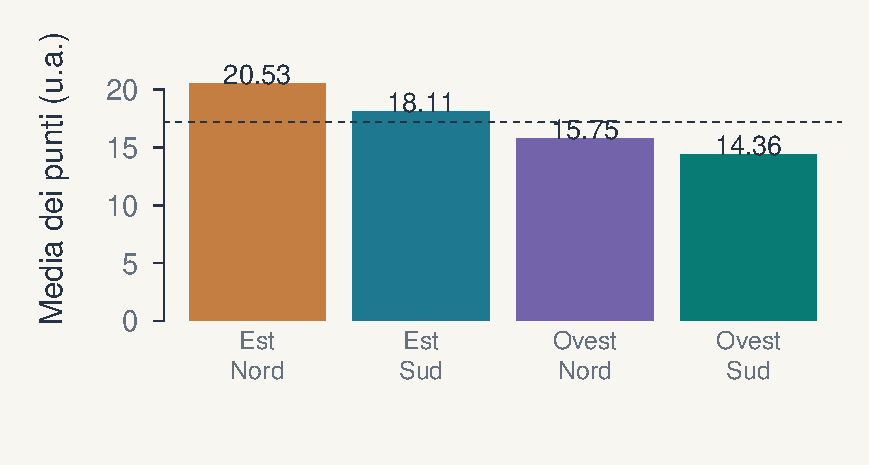
\includegraphics[width=9.85cm,height=5.25cm,keepaspectratio]{Risultati/Figure/30_medie_blocchi.pdf}
\vspace{1.5mm}
\PSmall{Quattro blocchi definiti dalle soglie $x=1000$ e $y=1000$ m; 16 siti in ciascuno.}
\[\bar z=\sum_b\frac{n_b}{n}\bar z_b\]

\end{minipage}\end{lrbox}
\typeout{FULLBOX:086:PilotLeftBox:\the\ht\PilotLeftBox:\the\dp\PilotLeftBox}

\begin{lrbox}{\PilotRightBox}
\begin{minipage}[t]{7.55cm}\raggedright\color{Ink}\fontsize{11.3}{14.8}\selectfont
\PBody{La media di tutti i siti è sempre la media delle medie di blocco pesata per le numerosità, quando ogni sito appartiene a un solo blocco.}
\vspace{2.5mm}
\PInfo{Se tutti gli $n_b$ sono uguali, i pesi sono uguali. La media non pesata dei blocchi coincide quindi con la media dei siti.}
\PCode{R · il caso bilanciato}{086_esempio.R}
\end{minipage}\end{lrbox}
\typeout{FULLBOX:086:PilotRightBox:\the\ht\PilotRightBox:\the\dp\PilotRightBox}

\begin{tikzpicture}[remember picture,overlay]
\PilotChrome{Con blocchi bilanciati le due medie coincidono}{VII · COPERTURA DEL CAMPIONE}{86}{L’uguaglianza fra media dei siti e media semplice dei blocchi dipende dal bilanciamento.}
\node[anchor=north west,inner sep=0] at([xshift=.96cm,yshift=-2.13cm]current page.north west){\usebox{\PilotLeftBox}};
\node[anchor=north west,inner sep=0] at([xshift=11.52cm,yshift=-2.13cm]current page.north west){\usebox{\PilotRightBox}};
\node[anchor=north east,inner sep=0] at([xshift=17.65cm,yshift=-12.06cm]current page.north west){\color{Classical}\fontsize{7.7}{9.2}\selectfont\href{../../03_Notebook_svolti/M11_Locus/M11_N17.html}{M11\_N17 · notebook svolto}};
\end{tikzpicture}\end{frame}

\begin{frame}[plain]\hypertarget{slide87}{}
\bookmark[level=1,page=87]{Con blocchi sbilanciati bisogna scegliere i pesi}
\begin{lrbox}{\TitleBox}
\begin{minipage}[t]{17.7cm}\raggedright\color{Ink}\fontsize{11.3}{14.8}\selectfont
\color{Navy}\bfseries\fontsize{20.6}{24.5}\selectfont Con blocchi sbilanciati bisogna scegliere i pesi
\end{minipage}\end{lrbox}
\typeout{FULLBOX:087:TitleBox:\the\ht\TitleBox:\the\dp\TitleBox}

\begin{lrbox}{\RecallBox}
\begin{minipage}[t]{14.3cm}\raggedright\color{Ink}\fontsize{11.3}{14.8}\selectfont
\fontsize{10.3}{13.8}\selectfont Il peso definisce quale popolazione viene rappresentata nella media.
\end{minipage}\end{lrbox}
\typeout{FULLBOX:087:RecallBox:\the\ht\RecallBox:\the\dp\RecallBox}

\begin{lrbox}{\PilotLeftBox}
\begin{minipage}[t]{10.05cm}\raggedright\color{Ink}\fontsize{11.3}{14.8}\selectfont
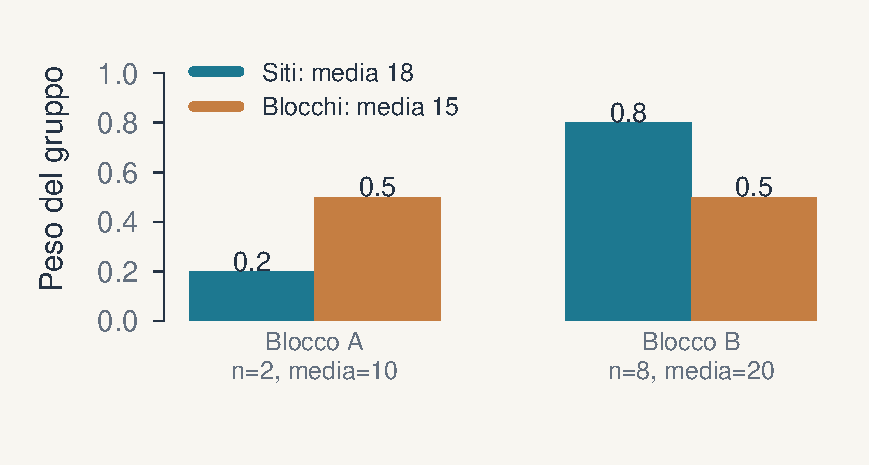
\includegraphics[width=9.85cm,height=4.3cm,keepaspectratio]{Risultati/Figure/31_pesi_squilibrati.pdf}
\vspace{1.5mm}
\PSmall{Esempio costruito: 2 osservazioni con media 10 e 8 osservazioni con media 20.}
\[\bar z_{\mathrm{siti}}=\frac{2\cdot10+8\cdot20}{10}=18\]
\[\bar z_{\mathrm{blocchi}}=\frac{10+20}{2}=15\]

\end{minipage}\end{lrbox}
\typeout{FULLBOX:087:PilotLeftBox:\the\ht\PilotLeftBox:\the\dp\PilotLeftBox}

\begin{lrbox}{\PilotRightBox}
\begin{minipage}[t]{7.55cm}\raggedright\color{Ink}\fontsize{11.3}{14.8}\selectfont
\PBody{La prima quantità assegna uguale peso ai siti. La seconda assegna uguale peso ai due blocchi.}
\vspace{2.5mm}
\PInfo{Nessuna delle due è una media areale per definizione. Per interpretarla come tale occorre collegare i blocchi alle aree rappresentate e al campionamento.}
\PCode{R · due bersagli distinti}{087_esempio.R}
\end{minipage}\end{lrbox}
\typeout{FULLBOX:087:PilotRightBox:\the\ht\PilotRightBox:\the\dp\PilotRightBox}

\begin{tikzpicture}[remember picture,overlay]
\PilotChrome{Con blocchi sbilanciati bisogna scegliere i pesi}{VII · COPERTURA DEL CAMPIONE}{87}{Il peso definisce quale popolazione viene rappresentata nella media.}
\node[anchor=north west,inner sep=0] at([xshift=.96cm,yshift=-2.13cm]current page.north west){\usebox{\PilotLeftBox}};
\node[anchor=north west,inner sep=0] at([xshift=11.52cm,yshift=-2.13cm]current page.north west){\usebox{\PilotRightBox}};
\node[anchor=north east,inner sep=0] at([xshift=17.65cm,yshift=-12.06cm]current page.north west){\color{Classical}\fontsize{7.7}{9.2}\selectfont\href{../../03_Notebook_svolti/M11_Locus/M11_N17.html}{M11\_N17 · notebook svolto}};
\end{tikzpicture}\end{frame}

\begin{frame}[plain]\hypertarget{slide88}{}
\bookmark[level=1,page=88]{La dipendenza entra nella varianza della media}
\begin{lrbox}{\TitleBox}
\begin{minipage}[t]{17.7cm}\raggedright\color{Ink}\fontsize{11.3}{14.8}\selectfont
\color{Navy}\bfseries\fontsize{20.6}{24.5}\selectfont La dipendenza entra nella varianza della media
\end{minipage}\end{lrbox}
\typeout{FULLBOX:088:TitleBox:\the\ht\TitleBox:\the\dp\TitleBox}

\begin{lrbox}{\RecallBox}
\begin{minipage}[t]{14.3cm}\raggedright\color{Ink}\fontsize{11.3}{14.8}\selectfont
\fontsize{10.3}{13.8}\selectfont La precisione della media dipende anche dalla relazione fra le osservazioni, oltre che dal loro numero.
\end{minipage}\end{lrbox}
\typeout{FULLBOX:088:RecallBox:\the\ht\RecallBox:\the\dp\RecallBox}

\begin{lrbox}{\PilotLeftBox}
\begin{minipage}[t]{10.05cm}\raggedright\color{Ink}\fontsize{11.3}{14.8}\selectfont
\[\operatorname{Var}(\bar Z)=\frac{1}{n^2}\sum_i\sum_j\operatorname{Cov}(Z_i,Z_j)\]
\[=\frac{1}{n^2}\left\{\sum_i\operatorname{Var}(Z_i)+2\sum_{i<j}\operatorname{Cov}(Z_i,Z_j)\right\}\]
\PInfo{La formula include i termini fra siti diversi. Con covarianze positive, ignorarli può sottostimare la varianza della media.}

\end{minipage}\end{lrbox}
\typeout{FULLBOX:088:PilotLeftBox:\the\ht\PilotLeftBox:\the\dp\PilotLeftBox}

\begin{lrbox}{\PilotRightBox}
\begin{minipage}[t]{7.55cm}\raggedright\color{Ink}\fontsize{11.3}{14.8}\selectfont
\PBody{Non esiste una numerosità effettiva universale ricavabile dal solo conteggio dei punti. Dipende dai pesi, dalla geometria e dalla covarianza del bersaglio.}
\vspace{2.5mm}
\PBody{La formula $\sigma^2/n$ è un caso particolare con varianze uguali e covarianze nulle fra osservazioni distinte.}
\vspace{2.5mm}

\end{minipage}\end{lrbox}
\typeout{FULLBOX:088:PilotRightBox:\the\ht\PilotRightBox:\the\dp\PilotRightBox}

\begin{tikzpicture}[remember picture,overlay]
\PilotChrome{La dipendenza entra nella varianza della media}{VII · COPERTURA DEL CAMPIONE}{88}{La precisione della media dipende anche dalla relazione fra le osservazioni, oltre che dal loro numero.}
\node[anchor=north west,inner sep=0] at([xshift=.96cm,yshift=-2.13cm]current page.north west){\usebox{\PilotLeftBox}};
\node[anchor=north west,inner sep=0] at([xshift=11.52cm,yshift=-2.13cm]current page.north west){\usebox{\PilotRightBox}};
\end{tikzpicture}\end{frame}

\begin{frame}[plain]\hypertarget{slide89}{}
\bookmark[level=1,page=89]{Nuovi campioni: copertura e piccole distanze}
\begin{lrbox}{\TitleBox}
\begin{minipage}[t]{17.7cm}\raggedright\color{Ink}\fontsize{11.3}{14.8}\selectfont
\color{Navy}\bfseries\fontsize{20.6}{24.5}\selectfont Nuovi campioni: copertura e piccole distanze
\end{minipage}\end{lrbox}
\typeout{FULLBOX:089:TitleBox:\the\ht\TitleBox:\the\dp\TitleBox}

\begin{lrbox}{\RecallBox}
\begin{minipage}[t]{14.3cm}\raggedright\color{Ink}\fontsize{11.3}{14.8}\selectfont
\fontsize{10.3}{13.8}\selectfont Copertura del dominio e informazione sulle piccole scale sono obiettivi complementari.
\end{minipage}\end{lrbox}
\typeout{FULLBOX:089:RecallBox:\the\ht\RecallBox:\the\dp\RecallBox}

\begin{lrbox}{\PilotLeftBox}
\begin{minipage}[t]{10.05cm}\raggedright\color{Ink}\fontsize{11.3}{14.8}\selectfont
{\fontsize{10.2}{13.1}\selectfont\renewcommand{\arraystretch}{1.45}\begin{tabular}{@{}p{4.0cm}p{5.0cm}@{}}\toprule
\textbf{Obiettivo} & \textbf{Posizioni utili da valutare}\\\midrule
Ridurre aree scoperte & Siti lontani dai campioni disponibili\\
Studiare piccole scale & Coppie ravvicinate e repliche progettate\\
Confrontare ambienti & Copertura degli strati scientifici\\
Verificare la previsione & Siti riservati secondo il compito\\
\bottomrule\end{tabular}}

\end{minipage}\end{lrbox}
\typeout{FULLBOX:089:PilotLeftBox:\the\ht\PilotLeftBox:\the\dp\PilotLeftBox}

\begin{lrbox}{\PilotRightBox}
\begin{minipage}[t]{7.55cm}\raggedright\color{Ink}\fontsize{11.3}{14.8}\selectfont
\PBody{Aggiungere soltanto siti molto distanti migliora la copertura, ma può lasciare poco informata la struttura a piccola scala. Aggiungere soltanto siti ravvicinati ha il limite opposto.}
\vspace{2.5mm}
\PInfo{Il disegno può combinare una copertura del dominio con coppie e repliche mirate. La scelta deve essere motivata rispetto al budget e alla domanda.}
\PBody{Le nuove misure vanno considerate prima della previsione finale se servono per scegliere il modello.}
\vspace{2.5mm}

\end{minipage}\end{lrbox}
\typeout{FULLBOX:089:PilotRightBox:\the\ht\PilotRightBox:\the\dp\PilotRightBox}

\begin{tikzpicture}[remember picture,overlay]
\PilotChrome{Nuovi campioni: copertura e piccole distanze}{VII · COPERTURA DEL CAMPIONE}{89}{Copertura del dominio e informazione sulle piccole scale sono obiettivi complementari.}
\node[anchor=north west,inner sep=0] at([xshift=.96cm,yshift=-2.13cm]current page.north west){\usebox{\PilotLeftBox}};
\node[anchor=north west,inner sep=0] at([xshift=11.52cm,yshift=-2.13cm]current page.north west){\usebox{\PilotRightBox}};
\end{tikzpicture}\end{frame}

\begin{frame}[plain]\hypertarget{slide90}{}
\bookmark[level=1,page=90]{La scheda del disegno rende visibili le esclusioni}
\begin{lrbox}{\TitleBox}
\begin{minipage}[t]{17.7cm}\raggedright\color{Ink}\fontsize{11.3}{14.8}\selectfont
\color{Navy}\bfseries\fontsize{20.6}{24.5}\selectfont La scheda del disegno rende visibili le esclusioni
\end{minipage}\end{lrbox}
\typeout{FULLBOX:090:TitleBox:\the\ht\TitleBox:\the\dp\TitleBox}

\begin{lrbox}{\RecallBox}
\begin{minipage}[t]{14.3cm}\raggedright\color{Ink}\fontsize{11.3}{14.8}\selectfont
\fontsize{10.3}{13.8}\selectfont Le esclusioni e il processo di selezione fanno parte dei dati necessari a interpretare l’analisi.
\end{minipage}\end{lrbox}
\typeout{FULLBOX:090:RecallBox:\the\ht\RecallBox:\the\dp\RecallBox}

\begin{lrbox}{\PilotLeftBox}
\begin{minipage}[t]{10.05cm}\raggedright\color{Ink}\fontsize{11.3}{14.8}\selectfont
{\fontsize{10.2}{13.1}\selectfont\renewcommand{\arraystretch}{1.45}\begin{tabular}{@{}p{3.4cm}p{5.6cm}@{}}\toprule
\textbf{Voce} & \textbf{Da registrare}\\\midrule
Dominio e supporto & Area, profondità, periodo della misura\\
Selezione & Procedura e probabilità note, se disponibili\\
Esclusioni & Siti inaccessibili o rimossi con motivo\\
Repliche & Sito, strumento e occasione di misura\\
Dati riservati & Regola geografica di separazione\\
\bottomrule\end{tabular}}

\end{minipage}\end{lrbox}
\typeout{FULLBOX:090:PilotLeftBox:\the\ht\PilotLeftBox:\the\dp\PilotLeftBox}

\begin{lrbox}{\PilotRightBox}
\begin{minipage}[t]{7.55cm}\raggedright\color{Ink}\fontsize{11.3}{14.8}\selectfont
\PBody{Una mappa dei siti mancanti può essere informativa quanto la mappa dei siti misurati. L’assenza di dati può dipendere da condizioni legate al fenomeno.}
\vspace{2.5mm}
\PInfo{La selezione per accessibilità non viene corretta automaticamente da un’interpolazione successiva.}
\PBody{La scheda distingue ciò che il campione rappresenta da ciò che si vorrebbe conoscere.}
\vspace{2.5mm}

\end{minipage}\end{lrbox}
\typeout{FULLBOX:090:PilotRightBox:\the\ht\PilotRightBox:\the\dp\PilotRightBox}

\begin{tikzpicture}[remember picture,overlay]
\PilotChrome{La scheda del disegno rende visibili le esclusioni}{VII · COPERTURA DEL CAMPIONE}{90}{Le esclusioni e il processo di selezione fanno parte dei dati necessari a interpretare l’analisi.}
\node[anchor=north west,inner sep=0] at([xshift=.96cm,yshift=-2.13cm]current page.north west){\usebox{\PilotLeftBox}};
\node[anchor=north west,inner sep=0] at([xshift=11.52cm,yshift=-2.13cm]current page.north west){\usebox{\PilotRightBox}};
\end{tikzpicture}\end{frame}

\begin{frame}[plain]\hypertarget{slide91}{}
\bookmark[level=1,page=91]{Laboratorio: campione e unità della sintesi}
\begin{lrbox}{\TitleBox}
\begin{minipage}[t]{17.7cm}\raggedright\color{Ink}\fontsize{11.3}{14.8}\selectfont
\color{Navy}\bfseries\fontsize{20.6}{24.5}\selectfont Laboratorio: campione e unità della sintesi
\end{minipage}\end{lrbox}
\typeout{FULLBOX:091:TitleBox:\the\ht\TitleBox:\the\dp\TitleBox}

\begin{lrbox}{\RecallBox}
\begin{minipage}[t]{14.3cm}\raggedright\color{Ink}\fontsize{11.3}{14.8}\selectfont
\fontsize{10.3}{13.8}\selectfont La media e la carta acquistano significato quando sono collegate a un bersaglio e a un disegno.
\end{minipage}\end{lrbox}
\typeout{FULLBOX:091:RecallBox:\the\ht\RecallBox:\the\dp\RecallBox}

\begin{lrbox}{\PilotLeftBox}
\begin{minipage}[t]{10.05cm}\raggedright\color{Ink}\fontsize{11.3}{14.8}\selectfont
\PLab{https://marzione00.github.io/Lab_Geo/\#laboratorio/m11-copertura}{Esperimento online · copertura geografica}
{\fontsize{10.2}{13.1}\selectfont\renewcommand{\arraystretch}{1.45}\begin{tabular}{@{}p{4.0cm}p{5.0cm}@{}}\toprule
\textbf{Attività} & \textbf{Risultato da discutere}\\\midrule
N16: strada & Media del corridoio e dominio escluso\\
Mappa della copertura & Aree e distanze poco rappresentate\\
N17: blocchi & Numerosità, medie e pesi\\
Esempio sbilanciato & 18 per sito, 15 per blocco\\
\bottomrule\end{tabular}}

\end{minipage}\end{lrbox}
\typeout{FULLBOX:091:PilotLeftBox:\the\ht\PilotLeftBox:\the\dp\PilotLeftBox}

\begin{lrbox}{\PilotRightBox}
\begin{minipage}[t]{7.55cm}\raggedright\color{Ink}\fontsize{11.3}{14.8}\selectfont
\PBody{La relazione finale deve nominare il bersaglio: media dei siti osservati, confronto fra blocchi o stima di una quantità territoriale.}
\vspace{2.5mm}
\PInfo{Nel dataset sintetico conosciamo tutti i 64 valori. Il confronto con una selezione serve a vedere una distorsione che, con soli dati parziali, potrebbe restare invisibile.}
\PBody{La previsione nello spazio deve rispettare gli stessi limiti di copertura.}
\vspace{2.5mm}

\end{minipage}\end{lrbox}
\typeout{FULLBOX:091:PilotRightBox:\the\ht\PilotRightBox:\the\dp\PilotRightBox}

\begin{tikzpicture}[remember picture,overlay]
\PilotChrome{Laboratorio: campione e unità della sintesi}{VII · COPERTURA DEL CAMPIONE}{91}{La media e la carta acquistano significato quando sono collegate a un bersaglio e a un disegno.}
\node[anchor=north west,inner sep=0] at([xshift=.96cm,yshift=-2.13cm]current page.north west){\usebox{\PilotLeftBox}};
\node[anchor=north west,inner sep=0] at([xshift=11.52cm,yshift=-2.13cm]current page.north west){\usebox{\PilotRightBox}};
\node[anchor=north east,inner sep=0] at([xshift=17.65cm,yshift=-12.06cm]current page.north west){\color{Classical}\fontsize{7.7}{9.2}\selectfont\href{../../03_Notebook_svolti/M11_Locus/M11_N17.html}{M11\_N17 · notebook svolto}};
\end{tikzpicture}\end{frame}

\begin{frame}[plain]\hypertarget{slide92}{}
\bookmark[level=0,page=92]{VIII · PREVISIONE SPAZIALE}
\bookmark[level=1,page=92]{IDW: prevedere con pesi di distanza}
\begin{lrbox}{\TitleBox}
\begin{minipage}[t]{17.7cm}\raggedright\color{Ink}\fontsize{11.3}{14.8}\selectfont
\color{Navy}\bfseries\fontsize{20.6}{24.5}\selectfont IDW: prevedere con pesi di distanza
\end{minipage}\end{lrbox}
\typeout{FULLBOX:092:TitleBox:\the\ht\TitleBox:\the\dp\TitleBox}

\begin{lrbox}{\RecallBox}
\begin{minipage}[t]{14.3cm}\raggedright\color{Ink}\fontsize{11.3}{14.8}\selectfont
\fontsize{10.3}{13.8}\selectfont IDW deve dichiarare metrica, esponente, campioni utilizzati e trattamento delle coincidenze.
\end{minipage}\end{lrbox}
\typeout{FULLBOX:092:RecallBox:\the\ht\RecallBox:\the\dp\RecallBox}

\begin{lrbox}{\PilotLeftBox}
\begin{minipage}[t]{10.05cm}\raggedright\color{Ink}\fontsize{11.3}{14.8}\selectfont
\[\widehat z(s_0)=\sum_iw_i(s_0)z_i\]
\[w_i(s_0)=\frac{d(s_i,s_0)^{-p}}{\sum_jd(s_j,s_0)^{-p}},\qquad p>0\]
\PInfo{La formula vale quando tutte le distanze dal bersaglio sono positive. La coincidenza con un campione richiede una regola separata.}

\end{minipage}\end{lrbox}
\typeout{FULLBOX:092:PilotLeftBox:\the\ht\PilotLeftBox:\the\dp\PilotLeftBox}

\begin{lrbox}{\PilotRightBox}
\begin{minipage}[t]{7.55cm}\raggedright\color{Ink}\fontsize{11.3}{14.8}\selectfont
\PBody{IDW assegna maggiore peso ai campioni vicini. L’esponente p regola la concentrazione dei pesi attorno al bersaglio.}
\vspace{2.5mm}
\PBody{È una regola di interpolazione. Non fornisce da sola un modello probabilistico dell’errore o un intervallo predittivo.}
\vspace{2.5mm}

\end{minipage}\end{lrbox}
\typeout{FULLBOX:092:PilotRightBox:\the\ht\PilotRightBox:\the\dp\PilotRightBox}

\begin{tikzpicture}[remember picture,overlay]
\PilotChrome{IDW: prevedere con pesi di distanza}{VIII · PREVISIONE SPAZIALE}{92}{IDW deve dichiarare metrica, esponente, campioni utilizzati e trattamento delle coincidenze.}
\node[anchor=north west,inner sep=0] at([xshift=.96cm,yshift=-2.13cm]current page.north west){\usebox{\PilotLeftBox}};
\node[anchor=north west,inner sep=0] at([xshift=11.52cm,yshift=-2.13cm]current page.north west){\usebox{\PilotRightBox}};
\node[anchor=north east,inner sep=0] at([xshift=17.65cm,yshift=-12.06cm]current page.north west){\color{Classical}\fontsize{7.7}{9.2}\selectfont\href{../../03_Notebook_svolti/M11_Locus/M11_N18.html}{M11\_N18 · notebook svolto}};
\end{tikzpicture}\end{frame}

\begin{frame}[plain]\hypertarget{slide93}{}
\bookmark[level=1,page=93]{Pesi positivi conservano costanti e intervalli}
\begin{lrbox}{\TitleBox}
\begin{minipage}[t]{17.7cm}\raggedright\color{Ink}\fontsize{11.3}{14.8}\selectfont
\color{Navy}\bfseries\fontsize{20.6}{24.5}\selectfont Pesi positivi conservano costanti e intervalli
\end{minipage}\end{lrbox}
\typeout{FULLBOX:093:TitleBox:\the\ht\TitleBox:\the\dp\TitleBox}

\begin{lrbox}{\RecallBox}
\begin{minipage}[t]{14.3cm}\raggedright\color{Ink}\fontsize{11.3}{14.8}\selectfont
\fontsize{10.3}{13.8}\selectfont I vincoli dei pesi spiegano sia proprietà utili sia limiti dell’interpolazione.
\end{minipage}\end{lrbox}
\typeout{FULLBOX:093:RecallBox:\the\ht\RecallBox:\the\dp\RecallBox}

\begin{lrbox}{\PilotLeftBox}
\begin{minipage}[t]{10.05cm}\raggedright\color{Ink}\fontsize{11.3}{14.8}\selectfont
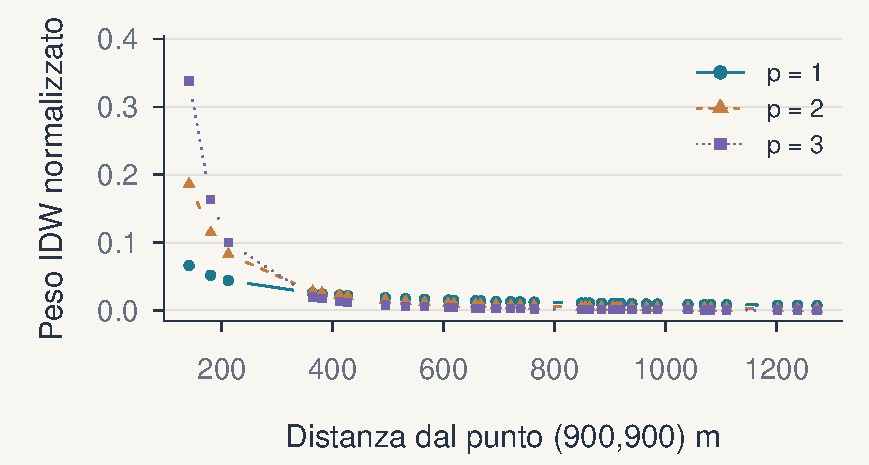
\includegraphics[width=9.85cm,height=5.25cm,keepaspectratio]{Risultati/Figure/32_idw_pesi.pdf}
\vspace{1.5mm}
\PSmall{Pesi verso $(900,900)$ m per p=1, 2 e 3. Ciascun vettore di pesi somma a uno.}
\[\min_i z_i\le\widehat z(s_0)\le\max_i z_i\]

\end{minipage}\end{lrbox}
\typeout{FULLBOX:093:PilotLeftBox:\the\ht\PilotLeftBox:\the\dp\PilotLeftBox}

\begin{lrbox}{\PilotRightBox}
\begin{minipage}[t]{7.55cm}\raggedright\color{Ink}\fontsize{11.3}{14.8}\selectfont
\PBody{Con pesi non negativi che sommano a uno, la previsione è una combinazione convessa dei valori utilizzati. Una variabile costante viene riprodotta.}
\vspace{2.5mm}
\PInfo{La proprietà non dimostra accuratezza. Fuori dall’area coperta dai dati, il vincolo può impedire di seguire un gradiente oltre i livelli osservati.}
\PCode{R · controllare i pesi}{093_esempio.R}
\end{minipage}\end{lrbox}
\typeout{FULLBOX:093:PilotRightBox:\the\ht\PilotRightBox:\the\dp\PilotRightBox}

\begin{tikzpicture}[remember picture,overlay]
\PilotChrome{Pesi positivi conservano costanti e intervalli}{VIII · PREVISIONE SPAZIALE}{93}{I vincoli dei pesi spiegano sia proprietà utili sia limiti dell’interpolazione.}
\node[anchor=north west,inner sep=0] at([xshift=.96cm,yshift=-2.13cm]current page.north west){\usebox{\PilotLeftBox}};
\node[anchor=north west,inner sep=0] at([xshift=11.52cm,yshift=-2.13cm]current page.north west){\usebox{\PilotRightBox}};
\node[anchor=north east,inner sep=0] at([xshift=17.65cm,yshift=-12.06cm]current page.north west){\color{Classical}\fontsize{7.7}{9.2}\selectfont\href{../../03_Notebook_svolti/M11_Locus/M11_N18.html}{M11\_N18 · notebook svolto}};
\end{tikzpicture}\end{frame}

\begin{frame}[plain]\hypertarget{slide94}{}
\bookmark[level=1,page=94]{L’esponente controlla quanto conta la vicinanza}
\begin{lrbox}{\TitleBox}
\begin{minipage}[t]{17.7cm}\raggedright\color{Ink}\fontsize{11.3}{14.8}\selectfont
\color{Navy}\bfseries\fontsize{20.6}{24.5}\selectfont L’esponente controlla quanto conta la vicinanza
\end{minipage}\end{lrbox}
\typeout{FULLBOX:094:TitleBox:\the\ht\TitleBox:\the\dp\TitleBox}

\begin{lrbox}{\RecallBox}
\begin{minipage}[t]{14.3cm}\raggedright\color{Ink}\fontsize{11.3}{14.8}\selectfont
\fontsize{10.3}{13.8}\selectfont La sensibilità all’esponente va valutata senza usare il test finale per scegliere il modello.
\end{minipage}\end{lrbox}
\typeout{FULLBOX:094:RecallBox:\the\ht\RecallBox:\the\dp\RecallBox}

\begin{lrbox}{\PilotLeftBox}
\begin{minipage}[t]{10.05cm}\raggedright\color{Ink}\fontsize{11.3}{14.8}\selectfont
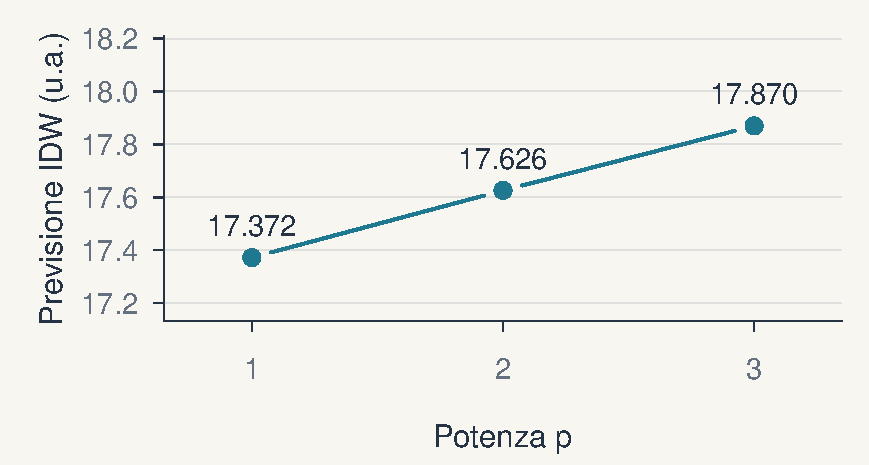
\includegraphics[width=9.85cm,height=5.25cm,keepaspectratio]{Risultati/Figure/33_idw_potenze.pdf}
\vspace{1.5mm}
\PSmall{Confronto dichiarato tra p=1, p=2 e p=3 sugli stessi campioni e bersagli.}

\end{minipage}\end{lrbox}
\typeout{FULLBOX:094:PilotLeftBox:\the\ht\PilotLeftBox:\the\dp\PilotLeftBox}

\begin{lrbox}{\PilotRightBox}
\begin{minipage}[t]{7.55cm}\raggedright\color{Ink}\fontsize{11.3}{14.8}\selectfont
\PBody{Valori maggiori di p concentrano il peso sui campioni più vicini. Valori più piccoli distribuiscono maggiormente l’influenza.}
\vspace{2.5mm}
\PInfo{Il valore esteticamente più gradevole non è necessariamente quello più accurato. Se p viene scelto dai dati, la scelta deve avvenire all’interno dell’addestramento.}
\PCode{R · confronto allo stesso bersaglio}{094_esempio.R}
\end{minipage}\end{lrbox}
\typeout{FULLBOX:094:PilotRightBox:\the\ht\PilotRightBox:\the\dp\PilotRightBox}

\begin{tikzpicture}[remember picture,overlay]
\PilotChrome{L’esponente controlla quanto conta la vicinanza}{VIII · PREVISIONE SPAZIALE}{94}{La sensibilità all’esponente va valutata senza usare il test finale per scegliere il modello.}
\node[anchor=north west,inner sep=0] at([xshift=.96cm,yshift=-2.13cm]current page.north west){\usebox{\PilotLeftBox}};
\node[anchor=north west,inner sep=0] at([xshift=11.52cm,yshift=-2.13cm]current page.north west){\usebox{\PilotRightBox}};
\node[anchor=north east,inner sep=0] at([xshift=17.65cm,yshift=-12.06cm]current page.north west){\color{Classical}\fontsize{7.7}{9.2}\selectfont\href{../../03_Notebook_svolti/M11_Locus/M11_N18.html}{M11\_N18 · notebook svolto}};
\end{tikzpicture}\end{frame}

\begin{frame}[plain]\hypertarget{slide95}{}
\bookmark[level=1,page=95]{Una superficie contiene previsioni, non nuovi dati}
\begin{lrbox}{\TitleBox}
\begin{minipage}[t]{17.7cm}\raggedright\color{Ink}\fontsize{11.3}{14.8}\selectfont
\color{Navy}\bfseries\fontsize{20.6}{24.5}\selectfont Una superficie contiene previsioni, non nuovi dati
\end{minipage}\end{lrbox}
\typeout{FULLBOX:095:TitleBox:\the\ht\TitleBox:\the\dp\TitleBox}

\begin{lrbox}{\RecallBox}
\begin{minipage}[t]{14.3cm}\raggedright\color{Ink}\fontsize{11.3}{14.8}\selectfont
\fontsize{10.3}{13.8}\selectfont Una griglia più fitta rende più fine il disegno, ma non aumenta l’informazione osservata.
\end{minipage}\end{lrbox}
\typeout{FULLBOX:095:RecallBox:\the\ht\RecallBox:\the\dp\RecallBox}

\begin{lrbox}{\FullWideBox}
\begin{minipage}[t]{18.1cm}\raggedright\color{Ink}\fontsize{11.3}{14.8}\selectfont
\centering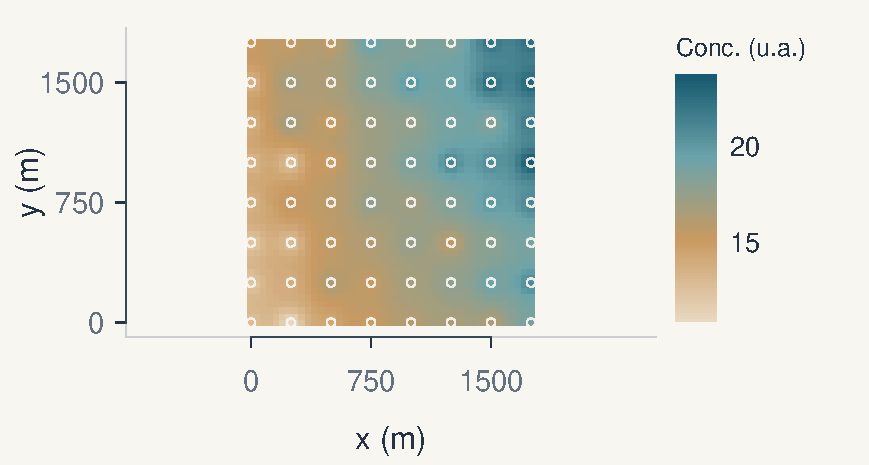
\includegraphics[width=18.05cm,height=5.8cm,keepaspectratio]{Risultati/Figure/34_idw_superficie.pdf}
\end{minipage}\end{lrbox}
\typeout{FULLBOX:095:FullWideBox:\the\ht\FullWideBox:\the\dp\FullWideBox}

\begin{lrbox}{\PilotRightBox}
\begin{minipage}[t]{18.1cm}\raggedright\color{Ink}\fontsize{11.3}{14.8}\selectfont
\PBody{IDW con p=2 sui 64 siti: la griglia di 45$\times$45 posizioni rende visibile la regola di interpolazione. I simboli indicano i campioni. Questa carta descrittiva usa l’intero dataset e non è la previsione del test geografico. La gestione delle coincidenze riproduce il valore osservato, oppure la media delle repliche coincidenti secondo la convenzione dichiarata.}
\end{minipage}\end{lrbox}
\typeout{FULLBOX:095:PilotRightBox:\the\ht\PilotRightBox:\the\dp\PilotRightBox}

\begin{tikzpicture}[remember picture,overlay]
\PilotChrome{Una superficie contiene previsioni, non nuovi dati}{VIII · PREVISIONE SPAZIALE}{95}{Una griglia più fitta rende più fine il disegno, ma non aumenta l’informazione osservata.}
\node[anchor=north west,inner sep=0] at([xshift=.96cm,yshift=-2.13cm]current page.north west){\usebox{\FullWideBox}};
\node[anchor=north west,inner sep=0] at([xshift=.96cm,yshift=-8.25cm]current page.north west){\usebox{\PilotRightBox}};
\node[anchor=north east,inner sep=0] at([xshift=17.65cm,yshift=-12.06cm]current page.north west){\color{Classical}\fontsize{7.7}{9.2}\selectfont\href{../../03_Notebook_svolti/M11_Locus/M11_N18.html}{M11\_N18 · notebook svolto}};
\end{tikzpicture}\end{frame}

\begin{frame}[plain]\hypertarget{slide96}{}
\bookmark[level=1,page=96]{Lasciare fuori Est verifica un trasferimento}
\begin{lrbox}{\TitleBox}
\begin{minipage}[t]{17.7cm}\raggedright\color{Ink}\fontsize{11.3}{14.8}\selectfont
\color{Navy}\bfseries\fontsize{20.6}{24.5}\selectfont Lasciare fuori Est verifica un trasferimento
\end{minipage}\end{lrbox}
\typeout{FULLBOX:096:TitleBox:\the\ht\TitleBox:\the\dp\TitleBox}

\begin{lrbox}{\RecallBox}
\begin{minipage}[t]{14.3cm}\raggedright\color{Ink}\fontsize{11.3}{14.8}\selectfont
\fontsize{10.3}{13.8}\selectfont La geometria della separazione determina quale capacità previsionale viene valutata.
\end{minipage}\end{lrbox}
\typeout{FULLBOX:096:RecallBox:\the\ht\RecallBox:\the\dp\RecallBox}

\begin{lrbox}{\PilotLeftBox}
\begin{minipage}[t]{10.05cm}\raggedright\color{Ink}\fontsize{11.3}{14.8}\selectfont
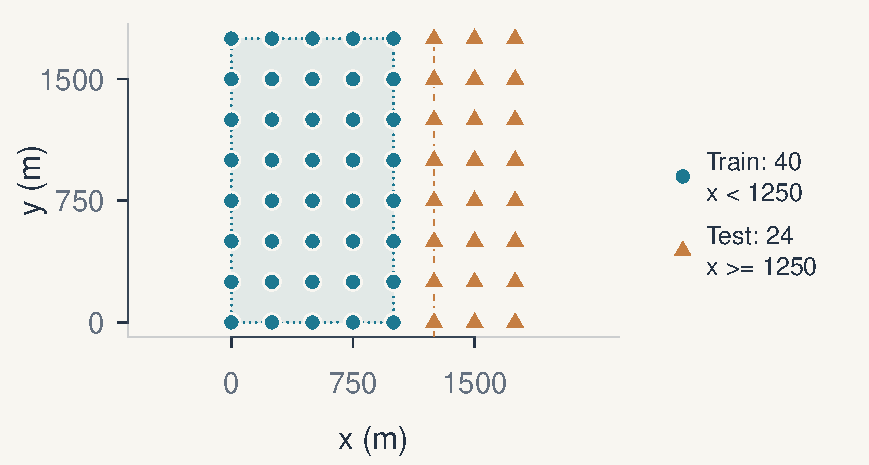
\includegraphics[width=9.85cm,height=5.25cm,keepaspectratio]{Risultati/Figure/35_split_spaziale.pdf}
\vspace{1.5mm}
\PSmall{Addestramento: $x<1250$ m, 40 siti. Test: $x\ge1250$ m, 24 siti. La linea $x=1250$ appartiene al test.}

\end{minipage}\end{lrbox}
\typeout{FULLBOX:096:PilotLeftBox:\the\ht\PilotLeftBox:\the\dp\PilotLeftBox}

\begin{lrbox}{\PilotRightBox}
\begin{minipage}[t]{7.55cm}\raggedright\color{Ink}\fontsize{11.3}{14.8}\selectfont
\PBody{I siti del test sono oltre l’estensione orientale del train. La prova valuta un trasferimento geografico, con extrapolazione verso Est.}
\vspace{2.5mm}
\PInfo{La geometria della separazione deve rappresentare il compito. Il protocollo principale fissa p=2 prima di leggere il test.}
\PCode{R · separazione geografica}{096_esempio.R}
\end{minipage}\end{lrbox}
\typeout{FULLBOX:096:PilotRightBox:\the\ht\PilotRightBox:\the\dp\PilotRightBox}

\begin{tikzpicture}[remember picture,overlay]
\PilotChrome{Lasciare fuori Est verifica un trasferimento}{VIII · PREVISIONE SPAZIALE}{96}{La geometria della separazione determina quale capacità previsionale viene valutata.}
\node[anchor=north west,inner sep=0] at([xshift=.96cm,yshift=-2.13cm]current page.north west){\usebox{\PilotLeftBox}};
\node[anchor=north west,inner sep=0] at([xshift=11.52cm,yshift=-2.13cm]current page.north west){\usebox{\PilotRightBox}};
\node[anchor=north east,inner sep=0] at([xshift=17.65cm,yshift=-12.06cm]current page.north west){\color{Classical}\fontsize{7.7}{9.2}\selectfont\href{../../03_Notebook_svolti/M11_Locus/M11_N19.html}{M11\_N19 · notebook svolto}};
\end{tikzpicture}\end{frame}

\begin{frame}[plain]\hypertarget{slide97}{}
\bookmark[level=1,page=97]{I riferimenti usano gli stessi campioni disponibili}
\begin{lrbox}{\TitleBox}
\begin{minipage}[t]{17.7cm}\raggedright\color{Ink}\fontsize{11.3}{14.8}\selectfont
\color{Navy}\bfseries\fontsize{20.6}{24.5}\selectfont I riferimenti usano gli stessi campioni disponibili
\end{minipage}\end{lrbox}
\typeout{FULLBOX:097:TitleBox:\the\ht\TitleBox:\the\dp\TitleBox}

\begin{lrbox}{\RecallBox}
\begin{minipage}[t]{14.3cm}\raggedright\color{Ink}\fontsize{11.3}{14.8}\selectfont
\fontsize{10.3}{13.8}\selectfont Metodi confrontabili devono prevedere gli stessi bersagli usando lo stesso insieme di informazioni.
\end{minipage}\end{lrbox}
\typeout{FULLBOX:097:RecallBox:\the\ht\RecallBox:\the\dp\RecallBox}

\begin{lrbox}{\PilotLeftBox}
\begin{minipage}[t]{10.05cm}\raggedright\color{Ink}\fontsize{11.3}{14.8}\selectfont
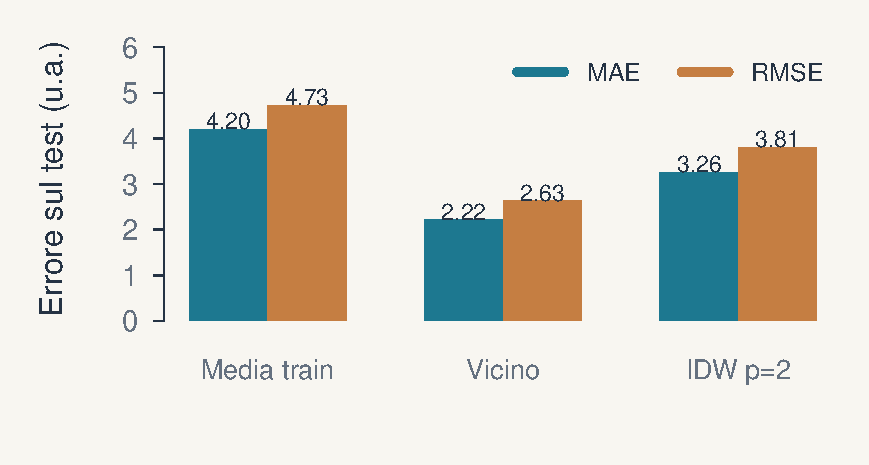
\includegraphics[width=9.85cm,height=5.25cm,keepaspectratio]{Risultati/Figure/36_previsioni_confronto.pdf}
\vspace{1.5mm}
\PSmall{Media dell’addestramento, vicino più prossimo e IDW p=2: stesso insieme di 24 siti da prevedere.}

\end{minipage}\end{lrbox}
\typeout{FULLBOX:097:PilotLeftBox:\the\ht\PilotLeftBox:\the\dp\PilotLeftBox}

\begin{lrbox}{\PilotRightBox}
\begin{minipage}[t]{7.55cm}\raggedright\color{Ink}\fontsize{11.3}{14.8}\selectfont
\PBody{RMSE sul test: vicino più prossimo 2,63, IDW 3,81, media del train 4,73 u.a. Il riferimento più semplice può quindi essere competitivo.}
\vspace{2.5mm}
\PInfo{IDW combina tutti i campioni del train con pesi di distanza. Nessuno dei tre metodi usa le concentrazioni del test per costruire la previsione.}
\PBody{Il vicino più prossimo è il migliore dei tre in questo test. La graduatoria riguarda questa geometria, questi dati e questa metrica.}
\vspace{2.5mm}

\end{minipage}\end{lrbox}
\typeout{FULLBOX:097:PilotRightBox:\the\ht\PilotRightBox:\the\dp\PilotRightBox}

\begin{tikzpicture}[remember picture,overlay]
\PilotChrome{I riferimenti usano gli stessi campioni disponibili}{VIII · PREVISIONE SPAZIALE}{97}{Metodi confrontabili devono prevedere gli stessi bersagli usando lo stesso insieme di informazioni.}
\node[anchor=north west,inner sep=0] at([xshift=.96cm,yshift=-2.13cm]current page.north west){\usebox{\PilotLeftBox}};
\node[anchor=north west,inner sep=0] at([xshift=11.52cm,yshift=-2.13cm]current page.north west){\usebox{\PilotRightBox}};
\node[anchor=north east,inner sep=0] at([xshift=17.65cm,yshift=-12.06cm]current page.north west){\color{Classical}\fontsize{7.7}{9.2}\selectfont\href{../../03_Notebook_svolti/M11_Locus/M11_N19.html}{M11\_N19 · notebook svolto}};
\end{tikzpicture}\end{frame}

\begin{frame}[plain]\hypertarget{slide98}{}
\bookmark[level=1,page=98]{Gli errori hanno grandezza, segno e posizione}
\begin{lrbox}{\TitleBox}
\begin{minipage}[t]{17.7cm}\raggedright\color{Ink}\fontsize{11.3}{14.8}\selectfont
\color{Navy}\bfseries\fontsize{20.6}{24.5}\selectfont Gli errori hanno grandezza, segno e posizione
\end{minipage}\end{lrbox}
\typeout{FULLBOX:098:TitleBox:\the\ht\TitleBox:\the\dp\TitleBox}

\begin{lrbox}{\RecallBox}
\begin{minipage}[t]{14.3cm}\raggedright\color{Ink}\fontsize{11.3}{14.8}\selectfont
\fontsize{10.3}{13.8}\selectfont Le metriche riassumono la prestazione; la carta degli errori ne mostra i limiti geografici.
\end{minipage}\end{lrbox}
\typeout{FULLBOX:098:RecallBox:\the\ht\RecallBox:\the\dp\RecallBox}

\begin{lrbox}{\PilotLeftBox}
\begin{minipage}[t]{10.05cm}\raggedright\color{Ink}\fontsize{11.3}{14.8}\selectfont
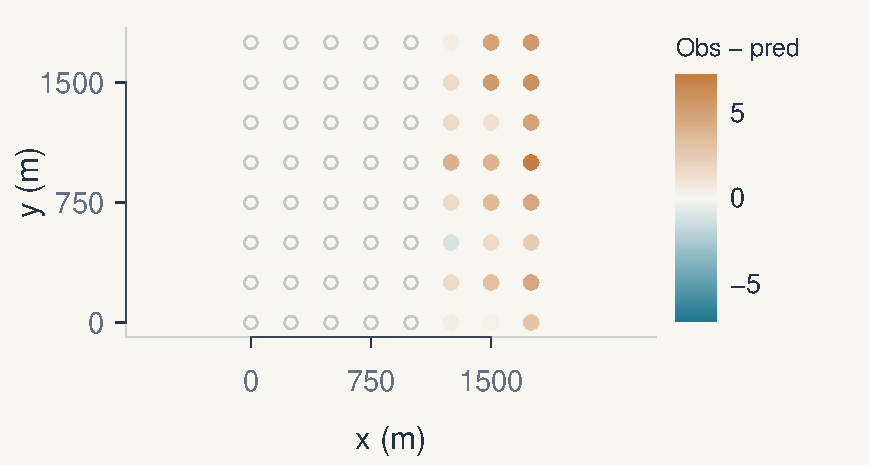
\includegraphics[width=9.85cm,height=5.0cm,keepaspectratio]{Risultati/Figure/37_errori_spaziali.pdf}
\vspace{1.5mm}
\PSmall{Errori $e_i=z_i-\widehat z_i$ nei siti tenuti fuori. Il segno positivo indica sottostima.}
\[\mathrm{MAE}=\frac1m\sum_i|e_i|,\qquad \mathrm{RMSE}=\sqrt{\frac1m\sum_ie_i^2}\]

\end{minipage}\end{lrbox}
\typeout{FULLBOX:098:PilotLeftBox:\the\ht\PilotLeftBox:\the\dp\PilotLeftBox}

\begin{lrbox}{\PilotRightBox}
\begin{minipage}[t]{7.55cm}\raggedright\color{Ink}\fontsize{11.3}{14.8}\selectfont
\PBody{Per IDW p=2, MAE=3,26 e bias=3,18 u.a. Il segno positivo indica una sottostima media dei siti Est.}
\vspace{2.5mm}
\PInfo{I 24 errori possono essere spazialmente dipendenti. Non sono 24 repliche indipendenti del protocollo di trasferimento.}
\PCode{R · valutare il test riservato}{098_esempio.R}
\end{minipage}\end{lrbox}
\typeout{FULLBOX:098:PilotRightBox:\the\ht\PilotRightBox:\the\dp\PilotRightBox}

\begin{tikzpicture}[remember picture,overlay]
\PilotChrome{Gli errori hanno grandezza, segno e posizione}{VIII · PREVISIONE SPAZIALE}{98}{Le metriche riassumono la prestazione; la carta degli errori ne mostra i limiti geografici.}
\node[anchor=north west,inner sep=0] at([xshift=.96cm,yshift=-2.13cm]current page.north west){\usebox{\PilotLeftBox}};
\node[anchor=north west,inner sep=0] at([xshift=11.52cm,yshift=-2.13cm]current page.north west){\usebox{\PilotRightBox}};
\node[anchor=north east,inner sep=0] at([xshift=17.65cm,yshift=-12.06cm]current page.north west){\color{Classical}\fontsize{7.7}{9.2}\selectfont\href{../../03_Notebook_svolti/M11_Locus/M11_N19.html}{M11\_N19 · notebook svolto}};
\end{tikzpicture}\end{frame}

\begin{frame}[plain]\hypertarget{slide99}{}
\bookmark[level=1,page=99]{Le scelte del modello restano dentro il train}
\begin{lrbox}{\TitleBox}
\begin{minipage}[t]{17.7cm}\raggedright\color{Ink}\fontsize{11.3}{14.8}\selectfont
\color{Navy}\bfseries\fontsize{20.6}{24.5}\selectfont Le scelte del modello restano dentro il train
\end{minipage}\end{lrbox}
\typeout{FULLBOX:099:TitleBox:\the\ht\TitleBox:\the\dp\TitleBox}

\begin{lrbox}{\RecallBox}
\begin{minipage}[t]{14.3cm}\raggedright\color{Ink}\fontsize{11.3}{14.8}\selectfont
\fontsize{10.3}{13.8}\selectfont La selezione dei parametri deve ricostruire una separazione spaziale coerente con il compito.
\end{minipage}\end{lrbox}
\typeout{FULLBOX:099:RecallBox:\the\ht\RecallBox:\the\dp\RecallBox}

\begin{lrbox}{\PilotLeftBox}
\begin{minipage}[t]{10.05cm}\raggedright\color{Ink}\fontsize{11.3}{14.8}\selectfont
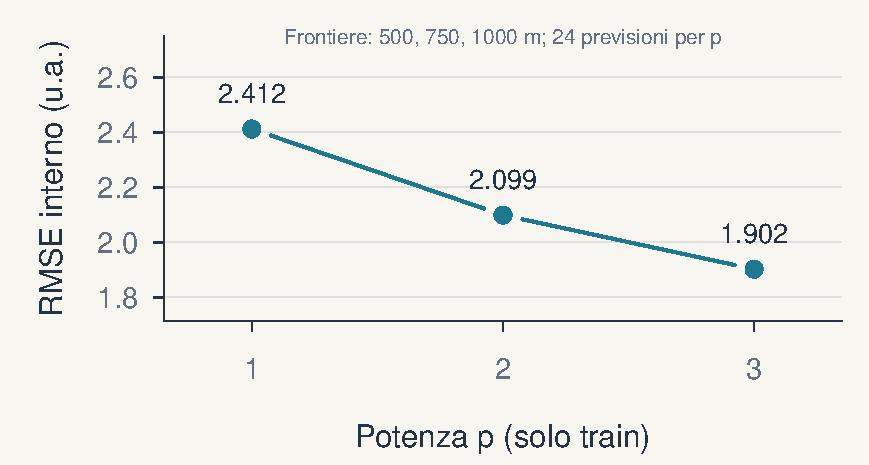
\includegraphics[width=9.85cm,height=5.25cm,keepaspectratio]{Risultati/Figure/38_tuning_blocchi.pdf}
\vspace{1.5mm}
\PSmall{Approfondimento: confronto degli esponenti con separazioni geografiche interne ai 40 siti di addestramento.}

\end{minipage}\end{lrbox}
\typeout{FULLBOX:099:PilotLeftBox:\the\ht\PilotLeftBox:\the\dp\PilotLeftBox}

\begin{lrbox}{\PilotRightBox}
\begin{minipage}[t]{7.55cm}\raggedright\color{Ink}\fontsize{11.3}{14.8}\selectfont
\PBody{Tre frontiere interne: x=500, 750 e 1000 m. Per ciascuna si stima sui siti a Ovest e si prevedono gli 8 siti della colonna alla frontiera.}
\vspace{2.5mm}
\PInfo{Si confrontano p=1, 2 e 3 su 24 previsioni interne con RMSE; viene scelto p=3. Il risultato principale sul test resta quello con p=2 prefissato, distinto dall’approfondimento.}
\PBody{Una partizione casuale può lasciare campioni molto vicini fra train e verifica e misurare un compito più facile del trasferimento ad Est.}
\vspace{2.5mm}

\end{minipage}\end{lrbox}
\typeout{FULLBOX:099:PilotRightBox:\the\ht\PilotRightBox:\the\dp\PilotRightBox}

\begin{tikzpicture}[remember picture,overlay]
\PilotChrome{Le scelte del modello restano dentro il train}{VIII · PREVISIONE SPAZIALE}{99}{La selezione dei parametri deve ricostruire una separazione spaziale coerente con il compito.}
\node[anchor=north west,inner sep=0] at([xshift=.96cm,yshift=-2.13cm]current page.north west){\usebox{\PilotLeftBox}};
\node[anchor=north west,inner sep=0] at([xshift=11.52cm,yshift=-2.13cm]current page.north west){\usebox{\PilotRightBox}};
\node[anchor=north east,inner sep=0] at([xshift=17.65cm,yshift=-12.06cm]current page.north west){\color{Classical}\fontsize{7.7}{9.2}\selectfont\href{../../03_Notebook_svolti/M11_Locus/M11_N19.html}{M11\_N19 · notebook svolto}};
\end{tikzpicture}\end{frame}

\begin{frame}[plain]\hypertarget{slide100}{}
\bookmark[level=1,page=100]{Il kriging aggiunge un modello di covarianza}
\begin{lrbox}{\TitleBox}
\begin{minipage}[t]{17.7cm}\raggedright\color{Ink}\fontsize{11.3}{14.8}\selectfont
\color{Navy}\bfseries\fontsize{20.6}{24.5}\selectfont Il kriging aggiunge un modello di covarianza
\end{minipage}\end{lrbox}
\typeout{FULLBOX:100:TitleBox:\the\ht\TitleBox:\the\dp\TitleBox}

\begin{lrbox}{\RecallBox}
\begin{minipage}[t]{14.3cm}\raggedright\color{Ink}\fontsize{11.3}{14.8}\selectfont
\fontsize{10.3}{13.8}\selectfont La proprietà di ottimalità del kriging è condizionata al modello della media e della covarianza.
\end{minipage}\end{lrbox}
\typeout{FULLBOX:100:RecallBox:\the\ht\RecallBox:\the\dp\RecallBox}

\begin{lrbox}{\PilotLeftBox}
\begin{minipage}[t]{10.05cm}\raggedright\color{Ink}\fontsize{11.3}{14.8}\selectfont
\[\widehat Z(s_0)=\sum_{i=1}^{m}\lambda_iY(s_i),\qquad \sum_i\lambda_i=1\]
{\fontsize{10.2}{13.1}\selectfont\renewcommand{\arraystretch}{1.45}\begin{tabular}{@{}p{4.0cm}p{5.0cm}@{}}\toprule
\textbf{Esempio verificabile} & \textbf{Specificazione}\\\midrule
Siti sulla linea & 0, 500, 1000 m\\
Valori osservati & 10, 15, 12 u.a.\\
Bersaglio & 250 m\\
Covarianza dichiarata & $C(h)=4\exp\{-(h/800)^2\}$\\
\bottomrule\end{tabular}}

\end{minipage}\end{lrbox}
\typeout{FULLBOX:100:PilotLeftBox:\the\ht\PilotLeftBox:\the\dp\PilotLeftBox}

\begin{lrbox}{\PilotRightBox}
\begin{minipage}[t]{7.55cm}\raggedright\color{Ink}\fontsize{11.3}{14.8}\selectfont
\PBody{Il kriging ordinario assume una media costante ignota. Cerca il predittore lineare non distorto con minima varianza dell’errore, sotto la covarianza specificata.}
\vspace{2.5mm}
\PInfo{Il piccolo esempio è separato dai dati con gradiente del caso guida. La covarianza è dichiarata per rendere controllabile il calcolo; non viene presentata come stimata dai tre valori.}
\PSmall{La linearità e la covarianza bastano per il criterio di minima varianza; intervalli gaussiani richiedono ulteriori assunzioni.}

\end{minipage}\end{lrbox}
\typeout{FULLBOX:100:PilotRightBox:\the\ht\PilotRightBox:\the\dp\PilotRightBox}

\begin{tikzpicture}[remember picture,overlay]
\PilotChrome{Il kriging aggiunge un modello di covarianza}{VIII · PREVISIONE SPAZIALE}{100}{La proprietà di ottimalità del kriging è condizionata al modello della media e della covarianza.}
\node[anchor=north west,inner sep=0] at([xshift=.96cm,yshift=-2.13cm]current page.north west){\usebox{\PilotLeftBox}};
\node[anchor=north west,inner sep=0] at([xshift=11.52cm,yshift=-2.13cm]current page.north west){\usebox{\PilotRightBox}};
\end{tikzpicture}\end{frame}

\begin{frame}[plain]\hypertarget{slide101}{}
\bookmark[level=1,page=101]{Il sistema impone la non distorsione}
\begin{lrbox}{\TitleBox}
\begin{minipage}[t]{17.7cm}\raggedright\color{Ink}\fontsize{11.3}{14.8}\selectfont
\color{Navy}\bfseries\fontsize{20.6}{24.5}\selectfont Il sistema impone la non distorsione
\end{minipage}\end{lrbox}
\typeout{FULLBOX:101:TitleBox:\the\ht\TitleBox:\the\dp\TitleBox}

\begin{lrbox}{\RecallBox}
\begin{minipage}[t]{14.3cm}\raggedright\color{Ink}\fontsize{11.3}{14.8}\selectfont
\fontsize{10.3}{13.8}\selectfont La matrice dei pesi nasce dal modello e dalla geometria, con un vincolo esplicito.
\end{minipage}\end{lrbox}
\typeout{FULLBOX:101:RecallBox:\the\ht\RecallBox:\the\dp\RecallBox}

\begin{lrbox}{\PilotLeftBox}
\begin{minipage}[t]{10.05cm}\raggedright\color{Ink}\fontsize{11.3}{14.8}\selectfont
\[\begin{bmatrix}C&\mathbf1\\\mathbf1^\top&0\end{bmatrix}\begin{bmatrix}\boldsymbol\lambda\\ \nu\end{bmatrix}=\begin{bmatrix}\boldsymbol c_0\\1\end{bmatrix}\]
{\fontsize{10.2}{13.1}\selectfont\renewcommand{\arraystretch}{1.45}\begin{tabular}{@{}p{3.2cm}p{5.8cm}@{}}\toprule
\textbf{Simbolo} & \textbf{Significato}\\\midrule
$C_{ij}$ & Covarianza fra osservazioni\\
$(c_0)_i$ & Covarianza fra osservazione e bersaglio\\
$\mathbf1^\top\lambda=1$ & Vincolo per la media costante ignota\\
$\nu$ & Moltiplicatore con il segno del sistema scritto\\
\bottomrule\end{tabular}}

\end{minipage}\end{lrbox}
\typeout{FULLBOX:101:PilotLeftBox:\the\ht\PilotLeftBox:\the\dp\PilotLeftBox}

\begin{lrbox}{\PilotRightBox}
\begin{minipage}[t]{7.55cm}\raggedright\color{Ink}\fontsize{11.3}{14.8}\selectfont
\PBody{Il sistema viene risolto insieme, senza calcolare esplicitamente l’inversa. Devono essere controllati soluzione, vincolo e stabilità numerica.}
\vspace{2.5mm}
\PInfo{La convenzione di segno del moltiplicatore deve restare coerente quando si scrive la varianza del kriging.}
\PCode{R · risolvere il sistema ordinario}{101_esempio.R}
\end{minipage}\end{lrbox}
\typeout{FULLBOX:101:PilotRightBox:\the\ht\PilotRightBox:\the\dp\PilotRightBox}

\begin{tikzpicture}[remember picture,overlay]
\PilotChrome{Il sistema impone la non distorsione}{VIII · PREVISIONE SPAZIALE}{101}{La matrice dei pesi nasce dal modello e dalla geometria, con un vincolo esplicito.}
\node[anchor=north west,inner sep=0] at([xshift=.96cm,yshift=-2.13cm]current page.north west){\usebox{\PilotLeftBox}};
\node[anchor=north west,inner sep=0] at([xshift=11.52cm,yshift=-2.13cm]current page.north west){\usebox{\PilotRightBox}};
\end{tikzpicture}\end{frame}

\begin{frame}[plain]\hypertarget{slide102}{}
\bookmark[level=1,page=102]{I pesi del kriging possono essere negativi}
\begin{lrbox}{\TitleBox}
\begin{minipage}[t]{17.7cm}\raggedright\color{Ink}\fontsize{11.3}{14.8}\selectfont
\color{Navy}\bfseries\fontsize{20.6}{24.5}\selectfont I pesi del kriging possono essere negativi
\end{minipage}\end{lrbox}
\typeout{FULLBOX:102:TitleBox:\the\ht\TitleBox:\the\dp\TitleBox}

\begin{lrbox}{\RecallBox}
\begin{minipage}[t]{14.3cm}\raggedright\color{Ink}\fontsize{11.3}{14.8}\selectfont
\fontsize{10.3}{13.8}\selectfont La somma dei pesi uguale a uno non basta a garantire una combinazione convessa.
\end{minipage}\end{lrbox}
\typeout{FULLBOX:102:RecallBox:\the\ht\RecallBox:\the\dp\RecallBox}

\begin{lrbox}{\PilotLeftBox}
\begin{minipage}[t]{10.05cm}\raggedright\color{Ink}\fontsize{11.3}{14.8}\selectfont
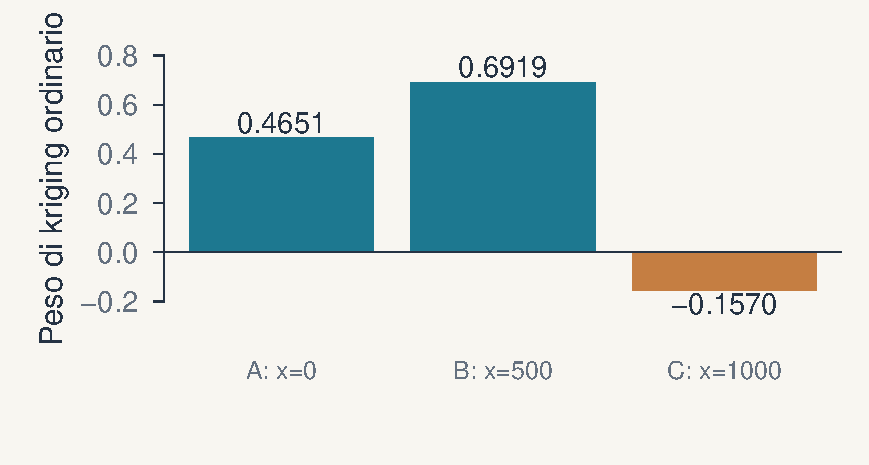
\includegraphics[width=9.85cm,height=5.25cm,keepaspectratio]{Risultati/Figure/39_kriging_pesi.pdf}
\vspace{1.5mm}
\PSmall{Nel caso dichiarato i tre pesi sommano a uno; il sito a 1000 m riceve un peso negativo.}

\end{minipage}\end{lrbox}
\typeout{FULLBOX:102:PilotLeftBox:\the\ht\PilotLeftBox:\the\dp\PilotLeftBox}

\begin{lrbox}{\PilotRightBox}
\begin{minipage}[t]{7.55cm}\raggedright\color{Ink}\fontsize{11.3}{14.8}\selectfont
\PBody{I pesi sono circa 0,465; 0,692; $-0,157$. La previsione è 13,145 u.a. La somma unitaria non impone la non negatività.}
\vspace{2.5mm}
\PInfo{Il kriging può produrre valori fuori dall’intervallo osservato. Un peso negativo non è automaticamente un errore: va letto nel contesto del modello.}
\PCode{R · leggere pesi e previsione}{102_esempio.R}
\end{minipage}\end{lrbox}
\typeout{FULLBOX:102:PilotRightBox:\the\ht\PilotRightBox:\the\dp\PilotRightBox}

\begin{tikzpicture}[remember picture,overlay]
\PilotChrome{I pesi del kriging possono essere negativi}{VIII · PREVISIONE SPAZIALE}{102}{La somma dei pesi uguale a uno non basta a garantire una combinazione convessa.}
\node[anchor=north west,inner sep=0] at([xshift=.96cm,yshift=-2.13cm]current page.north west){\usebox{\PilotLeftBox}};
\node[anchor=north west,inner sep=0] at([xshift=11.52cm,yshift=-2.13cm]current page.north west){\usebox{\PilotRightBox}};
\end{tikzpicture}\end{frame}

\begin{frame}[plain]\hypertarget{slide103}{}
\bookmark[level=1,page=103]{La varianza è condizionata alla covarianza scelta}
\begin{lrbox}{\TitleBox}
\begin{minipage}[t]{17.7cm}\raggedright\color{Ink}\fontsize{11.3}{14.8}\selectfont
\color{Navy}\bfseries\fontsize{20.6}{24.5}\selectfont La varianza è condizionata alla covarianza scelta
\end{minipage}\end{lrbox}
\typeout{FULLBOX:103:TitleBox:\the\ht\TitleBox:\the\dp\TitleBox}

\begin{lrbox}{\RecallBox}
\begin{minipage}[t]{14.3cm}\raggedright\color{Ink}\fontsize{11.3}{14.8}\selectfont
\fontsize{10.3}{13.8}\selectfont Una varianza di kriging va interpretata insieme alle ipotesi che la rendono calcolabile.
\end{minipage}\end{lrbox}
\typeout{FULLBOX:103:RecallBox:\the\ht\RecallBox:\the\dp\RecallBox}

\begin{lrbox}{\PilotLeftBox}
\begin{minipage}[t]{10.05cm}\raggedright\color{Ink}\fontsize{11.3}{14.8}\selectfont
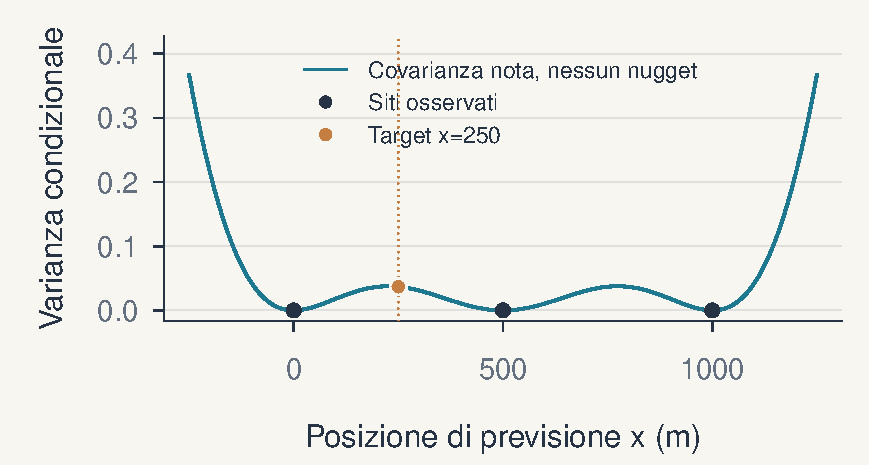
\includegraphics[width=9.85cm,height=5.25cm,keepaspectratio]{Risultati/Figure/40_kriging_varianza.pdf}
\vspace{1.5mm}
\PSmall{Varianza dell’errore per il campo dell’esempio, con covarianza nota e assenza di errore di misura.}
\[\sigma_K^2=C_{00}-2\lambda^\top c_0+\lambda^\top C\lambda\]

\end{minipage}\end{lrbox}
\typeout{FULLBOX:103:PilotLeftBox:\the\ht\PilotLeftBox:\the\dp\PilotLeftBox}

\begin{lrbox}{\PilotRightBox}
\begin{minipage}[t]{7.55cm}\raggedright\color{Ink}\fontsize{11.3}{14.8}\selectfont
\PBody{Nel bersaglio a 250 m la varianza è 0,03696 $(\mathrm{u.a.})^2$. Con il sistema scritto, coincide con $C_{00}-\lambda^\top c_0-\nu$.}
\vspace{2.5mm}
\PInfo{La varianza dipende da geometria, covarianza e bersaglio. Non include automaticamente l’incertezza dei parametri stimati o l’errore di scelta del modello.}
\PCode{R · verificare la varianza}{103_esempio.R}
\end{minipage}\end{lrbox}
\typeout{FULLBOX:103:PilotRightBox:\the\ht\PilotRightBox:\the\dp\PilotRightBox}

\begin{tikzpicture}[remember picture,overlay]
\PilotChrome{La varianza è condizionata alla covarianza scelta}{VIII · PREVISIONE SPAZIALE}{103}{Una varianza di kriging va interpretata insieme alle ipotesi che la rendono calcolabile.}
\node[anchor=north west,inner sep=0] at([xshift=.96cm,yshift=-2.13cm]current page.north west){\usebox{\PilotLeftBox}};
\node[anchor=north west,inner sep=0] at([xshift=11.52cm,yshift=-2.13cm]current page.north west){\usebox{\PilotRightBox}};
\end{tikzpicture}\end{frame}

\begin{frame}[plain]\hypertarget{slide104}{}
\bookmark[level=1,page=104]{Metodo e bersaglio devono restare coerenti}
\begin{lrbox}{\TitleBox}
\begin{minipage}[t]{17.7cm}\raggedright\color{Ink}\fontsize{11.3}{14.8}\selectfont
\color{Navy}\bfseries\fontsize{20.6}{24.5}\selectfont Metodo e bersaglio devono restare coerenti
\end{minipage}\end{lrbox}
\typeout{FULLBOX:104:TitleBox:\the\ht\TitleBox:\the\dp\TitleBox}

\begin{lrbox}{\RecallBox}
\begin{minipage}[t]{14.3cm}\raggedright\color{Ink}\fontsize{11.3}{14.8}\selectfont
\fontsize{10.3}{13.8}\selectfont La complessità del metodo non sostituisce coerenza del modello e verifica geografica.
\end{minipage}\end{lrbox}
\typeout{FULLBOX:104:RecallBox:\the\ht\RecallBox:\the\dp\RecallBox}

\begin{lrbox}{\PilotLeftBox}
\begin{minipage}[t]{10.05cm}\raggedright\color{Ink}\fontsize{11.3}{14.8}\selectfont
{\fontsize{10.2}{13.1}\selectfont\renewcommand{\arraystretch}{1.45}\begin{tabular}{@{}p{2.4cm}p{3.05cm}p{3.05cm}@{}}\toprule
\textbf{Aspetto} & \textbf{IDW} & \textbf{Kriging ordinario}\\\midrule
Pesi & Distanze e p & Covarianza e vincolo\\
Segno & Non negativi & Possono essere negativi\\
Media & Nessun modello esplicito & Costante ignota\\
Incertezza & Non fornita dalla regola & Condizionata al modello\\
\bottomrule\end{tabular}}

\end{minipage}\end{lrbox}
\typeout{FULLBOX:104:PilotLeftBox:\the\ht\PilotLeftBox:\the\dp\PilotLeftBox}

\begin{lrbox}{\PilotRightBox}
\begin{minipage}[t]{7.55cm}\raggedright\color{Ink}\fontsize{11.3}{14.8}\selectfont
\PBody{Per dati con un gradiente serve discutere il modello della media: per esempio covariate esplicite o una procedura di detrending coerente con la previsione.}
\vspace{2.5mm}
\PInfo{Prevedere un punto, una media di blocco o una nuova misura cambia covarianze e varianze coinvolte. Il bersaglio deve essere definito prima del calcolo.}
\PBody{La scelta del metodo richiede anche una verifica su dati tenuti fuori secondo una geometria appropriata.}
\vspace{2.5mm}

\end{minipage}\end{lrbox}
\typeout{FULLBOX:104:PilotRightBox:\the\ht\PilotRightBox:\the\dp\PilotRightBox}

\begin{tikzpicture}[remember picture,overlay]
\PilotChrome{Metodo e bersaglio devono restare coerenti}{VIII · PREVISIONE SPAZIALE}{104}{La complessità del metodo non sostituisce coerenza del modello e verifica geografica.}
\node[anchor=north west,inner sep=0] at([xshift=.96cm,yshift=-2.13cm]current page.north west){\usebox{\PilotLeftBox}};
\node[anchor=north west,inner sep=0] at([xshift=11.52cm,yshift=-2.13cm]current page.north west){\usebox{\PilotRightBox}};
\end{tikzpicture}\end{frame}

\begin{frame}[plain]\hypertarget{slide105}{}
\bookmark[level=1,page=105]{Laboratorio: prevedere senza usare il test}
\begin{lrbox}{\TitleBox}
\begin{minipage}[t]{17.7cm}\raggedright\color{Ink}\fontsize{11.3}{14.8}\selectfont
\color{Navy}\bfseries\fontsize{20.6}{24.5}\selectfont Laboratorio: prevedere senza usare il test
\end{minipage}\end{lrbox}
\typeout{FULLBOX:105:TitleBox:\the\ht\TitleBox:\the\dp\TitleBox}

\begin{lrbox}{\RecallBox}
\begin{minipage}[t]{14.3cm}\raggedright\color{Ink}\fontsize{11.3}{14.8}\selectfont
\fontsize{10.3}{13.8}\selectfont La verifica riguarda una procedura fissata e un compito geografico dichiarato.
\end{minipage}\end{lrbox}
\typeout{FULLBOX:105:RecallBox:\the\ht\RecallBox:\the\dp\RecallBox}

\begin{lrbox}{\PilotLeftBox}
\begin{minipage}[t]{10.05cm}\raggedright\color{Ink}\fontsize{11.3}{14.8}\selectfont
\PLab{https://marzione00.github.io/Lab_Geo/\#laboratorio/m11-interpolazione}{Esperimento online · interpolazione e verifica}
\PLab{https://marzione00.github.io/Lab_Geo/\#laboratorio/m11-kriging}{Esperimento online · kriging e incertezza}
{\fontsize{10.2}{13.1}\selectfont\renewcommand{\arraystretch}{1.45}\begin{tabular}{@{}p{3.7cm}p{5.3cm}@{}}\toprule
\textbf{Passaggio} & \textbf{Evidenza da conservare}\\\midrule
N18: IDW & Pesi, coincidenze, esponente, superficie\\
N19: test Est & 40 siti ammessi e 24 bersagli riservati\\
Confronto & Stesse metriche e stessi bersagli\\
Kriging illustrativo & Covarianza, sistema, pesi e varianza\\
Conclusione & Dominio di validità e limiti\\
\bottomrule\end{tabular}}

\end{minipage}\end{lrbox}
\typeout{FULLBOX:105:PilotLeftBox:\the\ht\PilotLeftBox:\the\dp\PilotLeftBox}

\begin{lrbox}{\PilotRightBox}
\begin{minipage}[t]{7.55cm}\raggedright\color{Ink}\fontsize{11.3}{14.8}\selectfont
\PBody{La carta sui 64 siti e il test costruito con i 40 siti del train ($x<1250$ m) devono rimanere riconoscibili. Sono due usi differenti dello stesso dataset.}
\vspace{2.5mm}
\PInfo{La consegna include errori per ID. Questo permette di verificare sia le metriche sia la loro distribuzione geografica.}
\PBody{Un risultato riproducibile conserva tutte le scelte necessarie a ricostruire la previsione.}
\vspace{2.5mm}

\end{minipage}\end{lrbox}
\typeout{FULLBOX:105:PilotRightBox:\the\ht\PilotRightBox:\the\dp\PilotRightBox}

\begin{tikzpicture}[remember picture,overlay]
\PilotChrome{Laboratorio: prevedere senza usare il test}{VIII · PREVISIONE SPAZIALE}{105}{La verifica riguarda una procedura fissata e un compito geografico dichiarato.}
\node[anchor=north west,inner sep=0] at([xshift=.96cm,yshift=-2.13cm]current page.north west){\usebox{\PilotLeftBox}};
\node[anchor=north west,inner sep=0] at([xshift=11.52cm,yshift=-2.13cm]current page.north west){\usebox{\PilotRightBox}};
\node[anchor=north east,inner sep=0] at([xshift=17.65cm,yshift=-12.06cm]current page.north west){\color{Classical}\fontsize{7.7}{9.2}\selectfont\href{../../03_Notebook_svolti/M11_Locus/M11_N19.html}{M11\_N19 · notebook svolto}};
\end{tikzpicture}\end{frame}

\begin{frame}[plain]\hypertarget{slide106}{}
\bookmark[level=0,page=106]{IX · CONSEGNA E STUDIO}
\bookmark[level=1,page=106]{Il progetto conserva dati, scelte e risultati}
\begin{lrbox}{\TitleBox}
\begin{minipage}[t]{17.7cm}\raggedright\color{Ink}\fontsize{11.3}{14.8}\selectfont
\color{Navy}\bfseries\fontsize{20.6}{24.5}\selectfont Il progetto conserva dati, scelte e risultati
\end{minipage}\end{lrbox}
\typeout{FULLBOX:106:TitleBox:\the\ht\TitleBox:\the\dp\TitleBox}

\begin{lrbox}{\RecallBox}
\begin{minipage}[t]{14.3cm}\raggedright\color{Ink}\fontsize{11.3}{14.8}\selectfont
\fontsize{10.3}{13.8}\selectfont Un risultato riproducibile conserva anche le convenzioni che collegano i numeri ai luoghi.
\end{minipage}\end{lrbox}
\typeout{FULLBOX:106:RecallBox:\the\ht\RecallBox:\the\dp\RecallBox}

\begin{lrbox}{\PilotLeftBox}
\begin{minipage}[t]{10.05cm}\raggedright\color{Ink}\fontsize{11.3}{14.8}\selectfont
{\fontsize{10.2}{13.1}\selectfont\renewcommand{\arraystretch}{1.45}\begin{tabular}{@{}p{3.4cm}p{5.6cm}@{}}\toprule
\textbf{Elemento} & \textbf{Contenuto minimo}\\\midrule
Dati & ID, unità, supporto, CRS e provenienza\\
Geometrie & Coordinate originali e trasformate\\
Relazioni & Metrica, soglia, matrice e ordine degli ID\\
Modelli & Formula, parametri, dominio di stima\\
Verifica & Separazione geografica ed errori per sito\\
Riproducibilità & Codice, versioni, risultati e limiti\\
\bottomrule\end{tabular}}

\end{minipage}\end{lrbox}
\typeout{FULLBOX:106:PilotLeftBox:\the\ht\PilotLeftBox:\the\dp\PilotLeftBox}

\begin{lrbox}{\PilotRightBox}
\begin{minipage}[t]{7.55cm}\raggedright\color{Ink}\fontsize{11.3}{14.8}\selectfont
\PBody{Il progetto parte da una domanda e termina con una conclusione circoscritta. Tabelle e figure devono permettere al lettore di verificare i passaggi.}
\vspace{2.5mm}
\PInfo{Il pacchetto contiene dati locali, sorgenti R, notebook eseguiti, figure e sorgenti XeLaTeX. Le mappe di raccordo collegano le nuove slide ai laboratori e alle pagine originali del sito.}
\PBody{Il file geografico di consegna viene riletto prima di essere considerato pronto.}
\vspace{2.5mm}

\end{minipage}\end{lrbox}
\typeout{FULLBOX:106:PilotRightBox:\the\ht\PilotRightBox:\the\dp\PilotRightBox}

\begin{tikzpicture}[remember picture,overlay]
\PilotChrome{Il progetto conserva dati, scelte e risultati}{IX · CONSEGNA E STUDIO}{106}{Un risultato riproducibile conserva anche le convenzioni che collegano i numeri ai luoghi.}
\node[anchor=north west,inner sep=0] at([xshift=.96cm,yshift=-2.13cm]current page.north west){\usebox{\PilotLeftBox}};
\node[anchor=north west,inner sep=0] at([xshift=11.52cm,yshift=-2.13cm]current page.north west){\usebox{\PilotRightBox}};
\node[anchor=north east,inner sep=0] at([xshift=17.65cm,yshift=-12.06cm]current page.north west){\color{Classical}\fontsize{7.7}{9.2}\selectfont\href{../../03_Notebook_svolti/M11_Locus/M11_N20.html}{M11\_N20 · notebook svolto}};
\end{tikzpicture}\end{frame}

\begin{frame}[plain]\hypertarget{slide107}{}
\bookmark[level=1,page=107]{GeoJSON: geometrie geografiche e attributi}
\begin{lrbox}{\TitleBox}
\begin{minipage}[t]{17.7cm}\raggedright\color{Ink}\fontsize{11.3}{14.8}\selectfont
\color{Navy}\bfseries\fontsize{20.6}{24.5}\selectfont GeoJSON: geometrie geografiche e attributi
\end{minipage}\end{lrbox}
\typeout{FULLBOX:107:TitleBox:\the\ht\TitleBox:\the\dp\TitleBox}

\begin{lrbox}{\RecallBox}
\begin{minipage}[t]{14.3cm}\raggedright\color{Ink}\fontsize{11.3}{14.8}\selectfont
\fontsize{10.3}{13.8}\selectfont La consegna geografica deve conservare sia le posizioni sia l’identità delle osservazioni.
\end{minipage}\end{lrbox}
\typeout{FULLBOX:107:RecallBox:\the\ht\RecallBox:\the\dp\RecallBox}

\begin{lrbox}{\PilotLeftBox}
\begin{minipage}[t]{10.05cm}\raggedright\color{Ink}\fontsize{11.3}{14.8}\selectfont
{\fontsize{10.2}{13.1}\selectfont\renewcommand{\arraystretch}{1.45}\begin{tabular}{@{}p{3.3cm}p{5.7cm}@{}}\toprule
\textbf{Campo} & \textbf{Convenzione della consegna}\\\midrule
Geometria & Point per ogni sito\\
Coordinate & Longitudine, latitudine in gradi\\
Riferimento & WGS 84 secondo RFC 7946\\
Attributi & ID, concentrazione, quota e area\\
Numero di elementi & 64 feature con ID univoci\\
\bottomrule\end{tabular}}

\end{minipage}\end{lrbox}
\typeout{FULLBOX:107:PilotLeftBox:\the\ht\PilotLeftBox:\the\dp\PilotLeftBox}

\begin{lrbox}{\PilotRightBox}
\begin{minipage}[t]{7.55cm}\raggedright\color{Ink}\fontsize{11.3}{14.8}\selectfont
\PBody{GeoJSON conforme a RFC 7946 usa WGS 84 in ordine longitudine--latitudine. Le coordinate locali in metri non devono essere interpretate come gradi.}
\vspace{2.5mm}
\PBody{Gli attributi restano associati agli ID.}
\vspace{2.5mm}
\PCode{R · scrivere e rileggere GeoJSON}{107_esempio.R}
\end{minipage}\end{lrbox}
\typeout{FULLBOX:107:PilotRightBox:\the\ht\PilotRightBox:\the\dp\PilotRightBox}

\begin{tikzpicture}[remember picture,overlay]
\PilotChrome{GeoJSON: geometrie geografiche e attributi}{IX · CONSEGNA E STUDIO}{107}{La consegna geografica deve conservare sia le posizioni sia l’identità delle osservazioni.}
\node[anchor=north west,inner sep=0] at([xshift=.96cm,yshift=-2.13cm]current page.north west){\usebox{\PilotLeftBox}};
\node[anchor=north west,inner sep=0] at([xshift=11.52cm,yshift=-2.13cm]current page.north west){\usebox{\PilotRightBox}};
\node[anchor=north east,inner sep=0] at([xshift=17.65cm,yshift=-12.06cm]current page.north west){\color{Classical}\fontsize{7.7}{9.2}\selectfont\href{../../03_Notebook_svolti/M11_Locus/M11_N20.html}{M11\_N20 · notebook svolto}};
\end{tikzpicture}\end{frame}

\begin{frame}[plain]\hypertarget{slide108}{}
\bookmark[level=1,page=108]{Rileggere verifica il contenuto consegnato}
\begin{lrbox}{\TitleBox}
\begin{minipage}[t]{17.7cm}\raggedright\color{Ink}\fontsize{11.3}{14.8}\selectfont
\color{Navy}\bfseries\fontsize{20.6}{24.5}\selectfont Rileggere verifica il contenuto consegnato
\end{minipage}\end{lrbox}
\typeout{FULLBOX:108:TitleBox:\the\ht\TitleBox:\the\dp\TitleBox}

\begin{lrbox}{\RecallBox}
\begin{minipage}[t]{14.3cm}\raggedright\color{Ink}\fontsize{11.3}{14.8}\selectfont
\fontsize{10.3}{13.8}\selectfont Una consegna è verificata quando il file riletto rappresenta le stesse osservazioni.
\end{minipage}\end{lrbox}
\typeout{FULLBOX:108:RecallBox:\the\ht\RecallBox:\the\dp\RecallBox}

\begin{lrbox}{\PilotLeftBox}
\begin{minipage}[t]{10.05cm}\raggedright\color{Ink}\fontsize{11.3}{14.8}\selectfont
{\fontsize{10.2}{13.1}\selectfont\renewcommand{\arraystretch}{1.45}\begin{tabular}{@{}p{3.4cm}p{5.6cm}@{}}\toprule
\textbf{Controllo} & \textbf{Esito atteso}\\\midrule
Conteggio & 64 feature\\
Identità & Stesso insieme di ID, senza duplicati\\
Attributi & Valori preservati con tolleranza dichiarata\\
Coordinate & Errore entro la precisione di scrittura\\
Riferimento & Geografico WGS 84\\
Versioni & R, sf, GDAL, GEOS e PROJ registrati\\
\bottomrule\end{tabular}}

\end{minipage}\end{lrbox}
\typeout{FULLBOX:108:PilotLeftBox:\the\ht\PilotLeftBox:\the\dp\PilotLeftBox}

\begin{lrbox}{\PilotRightBox}
\begin{minipage}[t]{7.55cm}\raggedright\color{Ink}\fontsize{11.3}{14.8}\selectfont
\PBody{La rilettura può cambiare l’ordine delle righe. Confrontiamo quindi le osservazioni dopo averle allineate per ID.}
\vspace{2.5mm}
\PInfo{La presenza del file non garantisce che contenga geometrie, attributi e riferimento corretti. Il controllo deve riguardare il contenuto.}
\PCode{R · controllo per identificativo}{108_esempio.R}
\end{minipage}\end{lrbox}
\typeout{FULLBOX:108:PilotRightBox:\the\ht\PilotRightBox:\the\dp\PilotRightBox}

\begin{tikzpicture}[remember picture,overlay]
\PilotChrome{Rileggere verifica il contenuto consegnato}{IX · CONSEGNA E STUDIO}{108}{Una consegna è verificata quando il file riletto rappresenta le stesse osservazioni.}
\node[anchor=north west,inner sep=0] at([xshift=.96cm,yshift=-2.13cm]current page.north west){\usebox{\PilotLeftBox}};
\node[anchor=north west,inner sep=0] at([xshift=11.52cm,yshift=-2.13cm]current page.north west){\usebox{\PilotRightBox}};
\node[anchor=north east,inner sep=0] at([xshift=17.65cm,yshift=-12.06cm]current page.north west){\color{Classical}\fontsize{7.7}{9.2}\selectfont\href{../../03_Notebook_svolti/M11_Locus/M11_N20.html}{M11\_N20 · notebook svolto}};
\end{tikzpicture}\end{frame}

\begin{frame}[plain]\hypertarget{slide109}{}
\bookmark[level=1,page=109]{I 20 notebook seguono il percorso della lezione}
\begin{lrbox}{\TitleBox}
\begin{minipage}[t]{17.7cm}\raggedright\color{Ink}\fontsize{11.3}{14.8}\selectfont
\color{Navy}\bfseries\fontsize{20.6}{24.5}\selectfont I 20 notebook seguono il percorso della lezione
\end{minipage}\end{lrbox}
\typeout{FULLBOX:109:TitleBox:\the\ht\TitleBox:\the\dp\TitleBox}

\begin{lrbox}{\RecallBox}
\begin{minipage}[t]{14.3cm}\raggedright\color{Ink}\fontsize{11.3}{14.8}\selectfont
\fontsize{10.3}{13.8}\selectfont Il codice serve a rendere controllabile l’argomento scientifico, non soltanto a produrre una figura.
\end{minipage}\end{lrbox}
\typeout{FULLBOX:109:RecallBox:\the\ht\RecallBox:\the\dp\RecallBox}

\begin{lrbox}{\PilotLeftBox}
\begin{minipage}[t]{10.05cm}\raggedright\color{Ink}\fontsize{11.3}{14.8}\selectfont
{\fontsize{10.2}{13.1}\selectfont\renewcommand{\arraystretch}{1.45}\begin{tabular}{@{}p{2.1cm}p{5.05cm}p{1.6cm}@{}}\toprule
\textbf{Notebook} & \textbf{Tema} & \textbf{Slide}\\\midrule
N01--N02 & Audit e ordine degli assi & 5--18\\
N03--N04 & Distanze nel piano e sulla sfera & 19--24\\
N05--N06 & Proiezione e rietichettatura & 25--31\\
N07--N10 & Carte, confini, join e buffer & 32--43\\
N11--N12 & Vicinati e matrici dei pesi & 44--55\\
N13--N14 & Moran e permutazioni & 56--70\\
N15 & Coppie e semivarianza & 71--81\\
N16--N17 & Copertura e medie di blocco & 82--91\\
N18--N20 & Previsione, verifica e consegna & 92--108\\
\bottomrule\end{tabular}}

\end{minipage}\end{lrbox}
\typeout{FULLBOX:109:PilotLeftBox:\the\ht\PilotLeftBox:\the\dp\PilotLeftBox}

\begin{lrbox}{\PilotRightBox}
\begin{minipage}[t]{7.55cm}\raggedright\color{Ink}\fontsize{11.3}{14.8}\selectfont
\PBody{Ogni notebook combina una domanda, il codice eseguito, risultati leggibili, controlli e commento scientifico. Gli HTML includono le risorse necessarie alla consultazione offline.}
\vspace{2.5mm}
\PInfo{I collegamenti nel piè di pagina aprono le attività corrispondenti nell’archivio estratto. Il formato R Markdown permette di modificare e rieseguire il lavoro.}
\PBody{Per studiare: ricostruire prima la previsione o il conteggio atteso; poi leggere il risultato ed esplicitare una possibile causa di errore.}
\vspace{2.5mm}

\end{minipage}\end{lrbox}
\typeout{FULLBOX:109:PilotRightBox:\the\ht\PilotRightBox:\the\dp\PilotRightBox}

\begin{tikzpicture}[remember picture,overlay]
\PilotChrome{I 20 notebook seguono il percorso della lezione}{IX · CONSEGNA E STUDIO}{109}{Il codice serve a rendere controllabile l’argomento scientifico, non soltanto a produrre una figura.}
\node[anchor=north west,inner sep=0] at([xshift=.96cm,yshift=-2.13cm]current page.north west){\usebox{\PilotLeftBox}};
\node[anchor=north west,inner sep=0] at([xshift=11.52cm,yshift=-2.13cm]current page.north west){\usebox{\PilotRightBox}};
\end{tikzpicture}\end{frame}

\begin{frame}[plain]\hypertarget{slide110}{}
\bookmark[level=1,page=110]{Una conclusione che conserva i luoghi}
\begin{lrbox}{\TitleBox}
\begin{minipage}[t]{17.7cm}\raggedright\color{Ink}\fontsize{11.3}{14.8}\selectfont
\color{Navy}\bfseries\fontsize{20.6}{24.5}\selectfont Una conclusione che conserva i luoghi
\end{minipage}\end{lrbox}
\typeout{FULLBOX:110:TitleBox:\the\ht\TitleBox:\the\dp\TitleBox}

\begin{lrbox}{\RecallBox}
\begin{minipage}[t]{14.3cm}\raggedright\color{Ink}\fontsize{11.3}{14.8}\selectfont
\fontsize{10.3}{13.8}\selectfont La posizione non è un accessorio del dato: entra nella domanda, nel modello e nella verifica.
\end{minipage}\end{lrbox}
\typeout{FULLBOX:110:RecallBox:\the\ht\RecallBox:\the\dp\RecallBox}

\begin{lrbox}{\PilotLeftBox}
\begin{minipage}[t]{10.05cm}\raggedright\color{Ink}\fontsize{11.3}{14.8}\selectfont
\begin{tikzpicture}[x=1cm,y=1cm]
\path[use as bounding box](-.1,-.15) rectangle(9.7,4.8);
\node[pFlow,text width=3.7cm,fill=GeoA!7] (a) at(2.1,3.7){Campioni e supporti};
\node[pFlow,text width=3.7cm,fill=GeoC!7] (b) at(7.3,3.7){Relazioni dichiarate};
\node[pFlow,text width=3.7cm,fill=GeoB!7] (c) at(2.1,1.15){Modello e bersaglio};
\node[pFlow,text width=3.7cm,fill=GeoA!7] (d) at(7.3,1.15){Verifica geografica};
\draw[pEdge] (a) -- (b);
\draw[pEdge] (a) -- (c);
\draw[pEdge] (b) -- (d);
\draw[pEdge] (c) -- (d);
\end{tikzpicture}
\PSmall{Riferimenti: documentazione \href{https://r-spatial.github.io/sf/}{sf}, \href{https://r-spatial.github.io/spdep/}{spdep}, \href{https://r-spatial.github.io/gstat/}{gstat}; \href{https://www.rfc-editor.org/rfc/rfc7946}{RFC 7946}. Fonti e convenzioni complete nel pacchetto.}

\end{minipage}\end{lrbox}
\typeout{FULLBOX:110:PilotLeftBox:\the\ht\PilotLeftBox:\the\dp\PilotLeftBox}

\begin{lrbox}{\PilotRightBox}
\begin{minipage}[t]{7.55cm}\raggedright\color{Ink}\fontsize{11.3}{14.8}\selectfont
\PBody{Una buona analisi spaziale tiene insieme ciò che è stato misurato, dove è stato misurato e quali relazioni sono state assunte.}
\vspace{2.5mm}
\PInfo{Prima di accettare una conclusione, chiedere: cambierebbe con un altro supporto, un altro vicinato o una diversa zona di verifica?}
\PBody{La carta finale deve rendere riconoscibili i campioni osservati, le quantità stimate e il territorio a cui la conclusione può essere riferita.}
\vspace{2.5mm}

\end{minipage}\end{lrbox}
\typeout{FULLBOX:110:PilotRightBox:\the\ht\PilotRightBox:\the\dp\PilotRightBox}

\begin{tikzpicture}[remember picture,overlay]
\PilotChrome{Una conclusione che conserva i luoghi}{IX · CONSEGNA E STUDIO}{110}{La posizione non è un accessorio del dato: entra nella domanda, nel modello e nella verifica.}
\node[anchor=north west,inner sep=0] at([xshift=.96cm,yshift=-2.13cm]current page.north west){\usebox{\PilotLeftBox}};
\node[anchor=north west,inner sep=0] at([xshift=11.52cm,yshift=-2.13cm]current page.north west){\usebox{\PilotRightBox}};
\end{tikzpicture}\end{frame}

\end{document}
